%----------------------------------------------------------------------------------------
%	LIBRO DE FÍSICA DE 2.º BACHILLERATO (español)
%   Compilar desde src/2BachFisica:
%   pdflatex -interaction=nonstopmode -synctex=1 -output-directory=../../out Fisica2BachLibroES.tex
%----------------------------------------------------------------------------------------
\documentclass[
    11pt, % Default font size, select one of 10pt, 11pt or 12pt
    %fleqn, % Left align equations
    a4paper, % Paper size, use either 'a4paper' for A4 size or 'letterpaper' for US letter size
%oneside, % Uncomment for oneside mode, this doesn't start new chapters and parts on odd pages (adding an empty page if required), this mode is more suitable if the book is to be read on a screen instead of printed
]{LegrandOrangeBookES}

\usepackage[spanish,es-noquoting,es-noshorthands,es-tabla]{babel}

\usepackage{estilocrispropioLibro}
\usepackage{longtable} % tablas largas con formato booktabs

% Color principal del libro: morado (Física 2.º Bachillerato). La clase y estilocrispropioLibro lo usan con el nombre «ocre».
\definecolor{ocre}{RGB}{94, 53, 177}

% Seno en español (por si babel no lo define)
\providecommand{\sen}{\operatorname{sen}}
\providecommand{\tg}{\operatorname{tg}}

\usepgfplotslibrary{fillbetween} % zonas sombreadas entre curvas (banda de estabilidad, UD8)

% Estilo de las gráficas de pgfplots del libro
\pgfplotsset{
    fisica/.style={
        width=0.32\linewidth, height=4.2cm,
        axis lines=middle, axis line style={-latex, thick},
        tick label style={font=\scriptsize}, label style={font=\small},
        every axis x label/.style={at={(ticklabel* cs:1)}, anchor=west},
        every axis y label/.style={at={(ticklabel* cs:1)}, anchor=south},
        samples=200, enlargelimits=false, clip=false,
    },
}

\hypersetup{
    pdftitle={Física 2.º Bachillerato}, % Title field
    pdfauthor={Cristóbal Melero}, % Author field
    pdfsubject={Física}, % Subject field
    pdfkeywords={Física, Bachillerato, movimiento armónico simple, ondas, óptica, gravitación, campo eléctrico, magnetismo, inducción, física cuántica, física nuclear}, % Keywords
    pdfcreator={LaTeX}, % Content creator field
}

\chapterimage{images/portada_cabeceras/cabecera_general} % Chapter heading image
\chapterspaceabove{6.5cm} % Default whitespace from the top of the page to the chapter title on chapter pages
\chapterspacebelow{6.75cm} % Default amount of vertical whitespace from the top margin to the start of the text on chapter pages

%----------------------------------------------------------------------------------------

\begin{document}
    % Fichero de soluciones propio, para no mezclarse en out/ con el soluciones.tex de los otros libros
    \Opensolutionfile{ans}[soluciones2BachFis]

%----------------------------------------------------------------------------------------
%	TITLE PAGE
%----------------------------------------------------------------------------------------

    \titlepage % Output the title page
    {\includegraphics[width=\paperwidth]{images/portada_cabeceras/portada_2BachFisica}} % Portada (PDF vectorial, fuente en images/portada_cabeceras/html/portada.html)

%----------------------------------------------------------------------------------------
%	COPYRIGHT PAGE
%----------------------------------------------------------------------------------------

    \thispagestyle{empty} % Suppress headers and footers on this page

    ~\vfill % Push the text down to the bottom of the page

    \noindent Copyright \copyright\ 2026 Cristóbal Melero\\ % Copyright notice

    \noindent \textsc{Published by CM Editorial}\\ % Publisher

    \noindent \textsc{\url{https://webfyq.com}}\\ % URL

    \noindent Licenciado bajo la licencia Creative Commons Atribución-NoComercial-CompartirIgual 4.0 Internacional (la ``Licencia''). No puede utilizar este archivo salvo en cumplimiento de la Licencia. Puede obtener una copia de la Licencia en \url{https://creativecommons.org/licenses/by-nc-sa/4.0}. Salvo que la legislación aplicable lo exija o se acuerde por escrito, el contenido distribuido bajo esta Licencia se proporciona \textsc{``tal cual'', sin garantías ni condiciones de ningún tipo}, ya sean expresas o implícitas. Consulte la Licencia para conocer el idioma específico que rige los permisos y las limitaciones establecidas en ella.\\

    \noindent \textit{Primera edición, 2026}

%----------------------------------------------------------------------------------------
%	TABLE OF CONTENTS
%----------------------------------------------------------------------------------------

    \pagestyle{empty} % Disable headers and footers for the following pages

    \tableofcontents % Output the table of contents

    \pagestyle{fancy} % Enable default headers and footers again

    \cleardoublepage % Start the following content on a new page

%----------------------------------------------------------------------------------------
%	PARTE: VIBRACIONES Y ONDAS
%----------------------------------------------------------------------------------------

    \part{Vibraciones y ondas}

    \chapterspaceabove{6.75cm} % Whitespace from the top of the page to the chapter title on chapter pages
    \chapterspacebelow{7.25cm} % Amount of vertical whitespace from the top margin to the start of the text on chapter pages

%------------------------------------------------

    \chapterimage{images/portada_cabeceras/cabecera_UD1}
    \chapter{Movimiento armónico simple}

    %! Unidad 1 — Movimiento armónico simple (teoría, actividades resueltas y prácticas)
%! Fuente: Fuentes/Tema1_Movimiento_Armonico_Simple.pdf (reescrito; datos de las actividades cambiados y recalculados)

\section*{Para empezar: el reloj de Huygens}
\addcontentsline{toc}{section}{Para empezar: el reloj de Huygens}

Hasta mediados del siglo \textsc{xvii} los mejores relojes mecánicos podían atrasarse o adelantarse un cuarto de hora al día.
En 1656 Christiaan Huygens construyó el primer reloj de péndulo: aprovechó que un péndulo que oscila con poca amplitud tarda
siempre lo mismo en ir y volver, y el error bajó a menos de un minuto diario. Ese «tardar siempre lo mismo» es la propiedad
central de esta unidad. Los muelles, los péndulos, las cuerdas de una guitarra, los átomos de un sólido o el aire que transmite
un sonido vibran de una forma muy parecida, y todos se describen con el mismo modelo: el \textbf{movimiento armónico simple}.
Además, es la base para estudiar las ondas en las unidades siguientes.

\section{Movimientos periódicos y oscilatorios}\label{sec:mas-periodico}

\begin{definition}[Movimiento periódico]
    Un movimiento es \rojon{periódico} cuando la posición, la velocidad y la aceleración del móvil vuelven a tomar los mismos
    valores a intervalos de tiempo iguales.
\end{definition}

Son periódicos, por ejemplo, el giro de las agujas de un reloj, la rotación de la Tierra o su traslación alrededor del Sol.

Un caso particular son los movimientos de ida y vuelta alrededor de una posición fija. Si separamos un cuerpo de su posición
de equilibrio \(O\) hasta \(A\) y lo soltamos, vuelve hacia \(O\), no se detiene allí, sigue hasta \(B\), se para un instante y
regresa hacia \(A\): \(A \rightarrow O \rightarrow B \rightarrow O \rightarrow A\) (figura~\ref{fig:mas-osciladores}).

\begin{figure}[H]
    \centering
    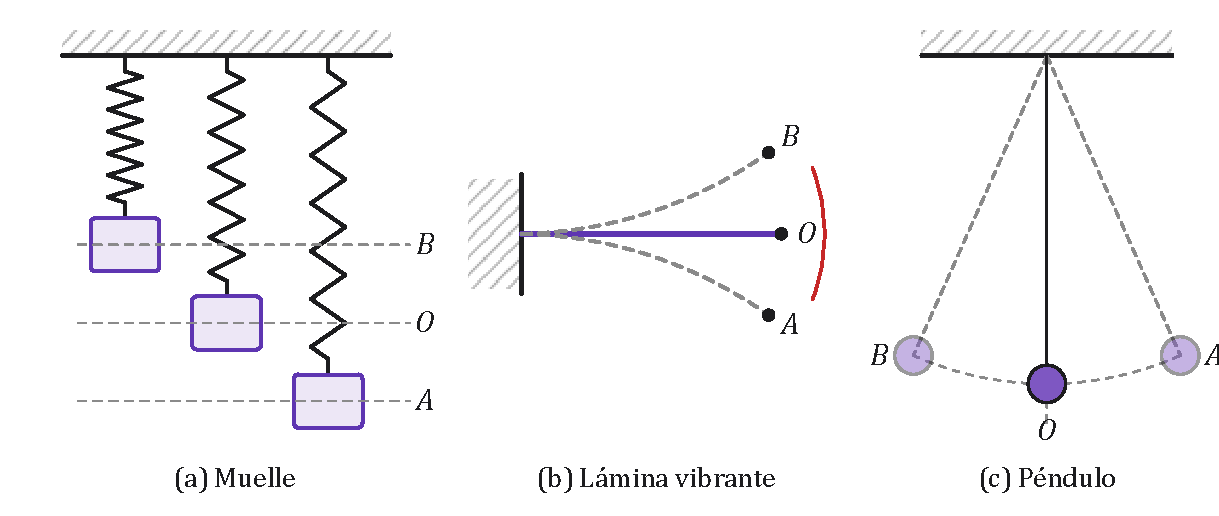
\includegraphics[width=0.9\linewidth]{images/UD1/osciladores}
    \caption{Tres osciladores: una masa colgada de un muelle, una lámina sujeta por un extremo y un péndulo. En los tres
    el cuerpo va y viene entre \(A\) y \(B\) pasando por la posición de equilibrio \(O\).}
    \label{fig:mas-osciladores}
\end{figure}

\begin{definition}[Movimiento oscilatorio]
    Un movimiento periódico es \rojon{oscilatorio} (o vibratorio) cuando el móvil va y viene a uno y otro lado de una posición
    de equilibrio. Cada recorrido completo de ida y vuelta (\(A \rightarrow O \rightarrow B \rightarrow O \rightarrow A\))
    se llama \azuln{oscilación}, \azuln{vibración} o \azuln{ciclo}.
\end{definition}

Para describir la rapidez con que se repite el movimiento se usan dos magnitudes, una inversa de la otra:
\begin{itemize}
    \item \textbf{Período} (\(T\)): tiempo que tarda el móvil en completar una oscilación. Se mide en segundos (\unit{\second}).
    \item \textbf{Frecuencia} (\(\nu\) o \(f\)): número de oscilaciones que realiza en cada unidad de tiempo. Se mide en hercios:
    \(\qty{1}{\hertz} = \qty{1}{\per\second}\) (una oscilación por segundo).
\end{itemize}
\begin{centeredequation}
    T = \dfrac{1}{\nu} \label{eq:mas-T-nu}
\end{centeredequation}

\section{El movimiento armónico simple}\label{sec:mas-definicion}

Entre todos los movimientos oscilatorios hay uno especialmente sencillo y frecuente en la naturaleza.

\begin{definition}[Movimiento armónico simple (m.a.s.)]
    Una partícula describe un \rojon{movimiento armónico simple} cuando oscila sobre un segmento rectilíneo y la fuerza que
    actúa sobre ella es, en cada instante, proporcional a su distancia a la posición de equilibrio y dirigida hacia ella:
    \begin{centeredequation}
        F = -k\,y \label{eq:mas-fuerza}
    \end{centeredequation}
    Esta fuerza se llama \azuln{fuerza recuperadora}. Un cuerpo que se mueve así es un \azuln{oscilador armónico}.
\end{definition}

El signo menos indica que la fuerza siempre apunta en sentido contrario al desplazamiento: si el cuerpo está por encima del
equilibrio (\(y > 0\)) la fuerza tira hacia abajo y si está por debajo (\(y < 0\)), hacia arriba. Como veremos, en un m.a.s. la
posición, la velocidad y la aceleración se expresan con funciones seno y coseno; por eso se llama \emph{armónico}.

\subsection{Magnitudes características}\label{subsec:mas-magnitudes}

\begin{table}[H]
    \centering
    \caption{Magnitudes que describen un movimiento armónico simple}
    \vspace{-5pt}
    \begin{tabular}{@{}lcL{8.2cm}c@{}}
        \toprule
        \textbf{Magnitud} & \textbf{Símbolo} & \textbf{Significado} & \makecell{\textbf{Unidad} \\ \textbf{(SI)}} \\
        \midrule
        Elongación & \(y\) & Posición del móvil medida desde el centro de oscilación (la posición de equilibrio). Puede ser positiva o negativa. & \unit{\m} \\[3pt]
        Amplitud & \(A\) & Valor máximo de la elongación. La distancia entre los dos extremos es \(2A\). & \unit{\m} \\[3pt]
        Período & \(T\) & Tiempo que dura una oscilación completa. & \unit{\second} \\[3pt]
        Frecuencia & \(\nu\) & Número de oscilaciones por segundo: \(\nu = 1/T\). & \unit{\hertz} \\[3pt]
        Pulsación & \(\omega\) & También llamada frecuencia angular: \(\omega = 2\pi/T = 2\pi\nu\). & \unit{\radian\per\second} \\[3pt]
        Fase & \(\omega t + \varphi_0\) & Ángulo que indica el estado de vibración en el instante \(t\). & \unit{\radian} \\[3pt]
        Fase inicial & \(\varphi_0\) & Valor de la fase en \(t = 0\); depende de dónde empieza el movimiento. & \unit{\radian} \\
        \bottomrule
    \end{tabular}
    \label{tab:mas-magnitudes}
\end{table}

\begin{remark}
    La pulsación se mide en \unit{\radian\per\second}, igual que una velocidad angular, pero no es una velocidad angular: en un
    m.a.s. nada gira. Se llama así porque, como veremos enseguida, el m.a.s. se puede obtener proyectando un movimiento circular.
\end{remark}

\section{Cinemática del movimiento armónico simple}\label{sec:mas-cinematica}

\subsection{Ecuación de la posición}\label{subsec:mas-posicion}

La ecuación del m.a.s. da la elongación en función del tiempo, \(y = f(t)\). Para obtenerla usaremos una idea muy útil:

\begin{center}
    \emph{El m.a.s. es la proyección sobre un diámetro de un movimiento circular uniforme.}
\end{center}

Imaginemos un punto \(P\) que recorre una circunferencia de radio \(A\) con velocidad angular constante \(\omega\), y su
sombra sobre el diámetro vertical (figura~\ref{fig:mas-mcu}). Mientras \(P\) da una vuelta, su sombra sube hasta \(+A\),
baja hasta \(-A\) y vuelve al centro: recorre el diámetro dos veces y hace una oscilación completa en el mismo tiempo \(T\)
que tarda \(P\) en dar la vuelta. En un cuarto de vuelta la sombra va del centro a un extremo: recorre la amplitud.

\begin{figure}[H]
    \centering
    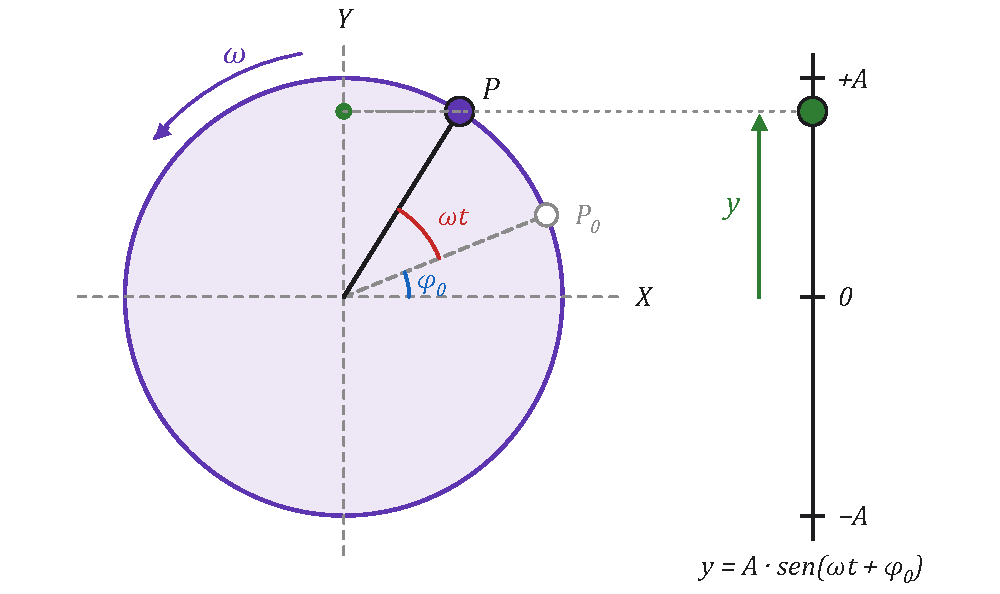
\includegraphics[width=0.72\linewidth]{images/UD1/mas_mcu}
    \caption{El punto \(P\) gira con velocidad angular \(\omega\). Su proyección sobre el diámetro vertical oscila entre
    \(+A\) y \(-A\) con un movimiento armónico simple.}
    \label{fig:mas-mcu}
\end{figure}

Si en \(t = 0\) el punto está en \(P_0\), formando un ángulo \(\varphi_0\) con el eje \(X\), en el instante \(t\) habrá girado
un ángulo \(\omega t\) más. La altura de su proyección es entonces:
\begin{centeredequation}
    \boxed{y = A \sen(\omega t + \varphi_0)} \label{eq:mas-posicion}
\end{centeredequation}

\begin{itemize}
    \item \(A\), \(\omega\) y \(\varphi_0\) son constantes que hay que conocer para escribir la ecuación de un m.a.s. concreto.
    \item \(\omega t + \varphi_0\) es la \azuln{fase}: determina el estado de vibración (posición y sentido del movimiento) en cada instante.
    \item \(\varphi_0\) es la \azuln{fase inicial}. Se calcula con las condiciones iniciales, es decir, con la posición (y el
    sentido del movimiento) en \(t = 0\).
\end{itemize}

Si proyectamos sobre el eje horizontal se obtiene \(x = A\cos(\omega t + \varphi_0)\). Ambas formas son equivalentes (solo
cambia el valor de \(\varphi_0\), porque \(\cos\alpha = \sen(\alpha + \pi/2)\)); en este libro usaremos la del seno.

\begin{remark}
    En las ecuaciones del m.a.s. los ángulos están en radianes: \textbf{hay que poner la calculadora en modo RAD}.
\end{remark}

\paragraph{Puntos en fase y en oposición de fase.} La diferencia de fase entre dos instantes \(t_1\) y \(t_2\) del mismo
movimiento es:
\begin{equation*}
    \Delta\varphi = (\omega t_2 + \varphi_0) - (\omega t_1 + \varphi_0) = \omega\,(t_2 - t_1) = \omega\,\Delta t
\end{equation*}
\begin{itemize}
    \item Están \rojon{en fase} si \(\Delta\varphi = 2n\pi\) (\(n = 1, 2, 3\ldots\)): el móvil está en la misma posición y se
    mueve en el mismo sentido. Ocurre cuando \(\Delta t = nT\).
    \item Están \rojon{en oposición de fase} si \(\Delta\varphi = (2n-1)\pi\): las elongaciones son opuestas y el móvil se
    mueve en sentidos contrarios.
\end{itemize}

\begin{exercise}
    ¿Qué intervalo de tiempo separa dos instantes en los que un m.a.s. está en oposición de fase?
    \begin{solu}
        \textcolor{blue}{En oposición de fase \(\Delta\varphi = (2n-1)\pi\). Como \(\Delta\varphi = \omega\,\Delta t = \dfrac{2\pi}{T}\,\Delta t\):}
        \[ \dfrac{2\pi}{T}\,\Delta t = (2n-1)\pi \quad\Rightarrow\quad \textcolor{red}{\Delta t = (2n-1)\,\dfrac{T}{2}} \]
        \textcolor{red}{Un número impar de medios períodos: \(T/2\), \(3T/2\), \(5T/2\ldots\)}
    \end{solu}
\end{exercise}

\begin{exercise}
    Un cuerpo colgado de un muelle oscila con un m.a.s. de \qty{12}{\cm} de amplitud y \qty{0.2}{\second} de período. En
    \(t = 0\) el muelle está en su máximo alargamiento, que tomamos como elongación negativa. Escribe la ecuación del movimiento.
    \begin{solu}
        \textcolor{blue}{Ecuación general: \(y = A\sen(\omega t + \varphi_0)\), con \(A = \qty{0.12}{\m}\).}

        \textcolor{blue}{Pulsación: \(\omega = \dfrac{2\pi}{T} = \dfrac{2\pi}{0{,}2} = 10\pi\ \unit{\radian\per\second}\).}

        \textcolor{blue}{Fase inicial: en \(t = 0\), \(y = -A\): \(-0{,}12 = 0{,}12 \sen\varphi_0 \Rightarrow \sen\varphi_0 = -1
        \Rightarrow \varphi_0 = \dfrac{3\pi}{2}\ \unit{\radian}\).}
        \[ \textcolor{red}{y = 0{,}12\,\sen\!\left(10\pi t + \dfrac{3\pi}{2}\right)\ \text{(m)}} \]
    \end{solu}
\end{exercise}

\begin{exercise}
    Una partícula con m.a.s. sale del extremo positivo de su trayectoria y tarda \qty{0.5}{\second} en llegar al centro, que
    está a \qty{15}{\cm}. Calcula:
    \begin{enumerate}[label=\letraminuscula]
        \item La frecuencia.
        \item La ecuación del movimiento.
        \item La posición \qty{1}{\second} después de empezar.
    \end{enumerate}
    \begin{solu}
        \textcolor{blue}{Del extremo al centro hay un cuarto de oscilación: \(T/4 = \qty{0.5}{\second} \Rightarrow T = \qty{2}{\second}\);
        y la distancia es la amplitud: \(A = \qty{0.15}{\m}\).}
        \begin{enumerate}[label=\letraminuscula]
            \item \(\nu = \dfrac{1}{T} = \textcolor{red}{\qty{0.5}{\hertz}}\).
            \item \textcolor{blue}{\(\omega = 2\pi/T = \pi\ \unit{\radian\per\second}\). En \(t = 0\), \(y = A\): \(\sen\varphi_0 = 1 \Rightarrow \varphi_0 = \pi/2\).}
            \(\textcolor{red}{y = 0{,}15\,\sen\!\left(\pi t + \dfrac{\pi}{2}\right)\ \text{(m)}}\)
            \item \(y(1) = 0{,}15\,\sen\!\left(\pi + \dfrac{\pi}{2}\right) = 0{,}15\cdot(-1) = \textcolor{red}{\qty{-0.15}{\m}}\):
            al cabo de medio período está en el otro extremo.
        \end{enumerate}
    \end{solu}
\end{exercise}

\begin{exercise}
    Una partícula con m.a.s. recorre un segmento de \qty{10}{\cm} (de un extremo al otro) en \qty{0.04}{\second}. En \(t = 0\)
    su elongación es máxima y positiva. Calcula:
    \begin{enumerate}[label=\letraminuscula]
        \item La ecuación del movimiento.
        \item La posición en \(t = \qty{1.3}{\second}\).
        \item La diferencia de fase entre ese instante y el inicial.
    \end{enumerate}
    \begin{solu}
        \textcolor{blue}{Datos: \(2A = \qty{10}{\cm} \Rightarrow A = \qty{0.05}{\m}\). Ir de un extremo al otro es media
        oscilación: \(T/2 = \qty{0.04}{\second} \Rightarrow T = \qty{0.08}{\second}\).}
        \begin{enumerate}[label=\letraminuscula]
            \item \textcolor{blue}{\(\omega = \dfrac{2\pi}{0{,}08} = 25\pi\ \unit{\radian\per\second}\); con \(y(0) = A\), \(\varphi_0 = \pi/2\).}
            \(\textcolor{red}{y = 0{,}05\,\sen\!\left(25\pi t + \dfrac{\pi}{2}\right)\ \text{(m)}}\)
            \item \(y(1{,}3) = 0{,}05\,\sen(32{,}5\pi + 0{,}5\pi) = 0{,}05\,\sen(33\pi) = \textcolor{red}{0}\): pasa por el centro.
            \item \(\Delta\varphi = \omega\,\Delta t = 25\pi\cdot 1{,}3 = \textcolor{red}{32{,}5\pi\ \unit{\radian}}\).
        \end{enumerate}
    \end{solu}
\end{exercise}

\subsection{Ecuación de la velocidad}\label{subsec:mas-velocidad}

La velocidad es la derivada de la posición respecto del tiempo:
\begin{centeredequation}
    \boxed{v = \dfrac{dy}{dt} = A\,\omega\cos(\omega t + \varphi_0)} \label{eq:mas-velocidad}
\end{centeredequation}

Usando \(\sen^2\alpha + \cos^2\alpha = 1\) podemos expresarla en función de la posición:
\begin{equation*}
    v = \pm A\omega\sqrt{1 - \sen^2(\omega t + \varphi_0)} = \pm\,\omega\sqrt{A^2 - A^2\sen^2(\omega t + \varphi_0)}
    \quad\Rightarrow\quad \boxed{v = \pm\,\omega\sqrt{A^2 - y^2}}
\end{equation*}
El signo depende del sentido en que se mueve el cuerpo. La velocidad:
\begin{itemize}
    \item es \textbf{máxima} en el centro (\(y = 0\)): \(v_{\text{máx}} = A\,\omega\);
    \item es \textbf{nula} en los extremos (\(y = \pm A\)), donde el cuerpo se para para cambiar de sentido.
\end{itemize}

\begin{exercise}
    Un m.a.s. tiene por ecuación \(y = 0{,}3\,\sen(4\pi t + \pi)\) (SI). Calcula:
    \begin{enumerate}[label=\letraminuscula]
        \item La amplitud, la pulsación, el período, la frecuencia y la fase inicial.
        \item La velocidad en \(t = 0\), la velocidad máxima y la velocidad en \(t = \qty{0.5}{\second}\).
    \end{enumerate}
    \begin{solu}
        \begin{enumerate}[label=\letraminuscula]
            \item \textcolor{blue}{Comparando con \(y = A\sen(\omega t + \varphi_0)\):}
            \textcolor{red}{\(A = \qty{0.3}{\m}\); \(\omega = 4\pi\ \unit{\radian\per\second}\); \(T = \dfrac{2\pi}{4\pi} = \qty{0.5}{\second}\);
            \(\nu = \qty{2}{\hertz}\); \(\varphi_0 = \pi\ \unit{\radian}\).}
            \item \textcolor{blue}{\(v = A\omega\cos(\omega t + \varphi_0) = 1{,}2\pi\cos(4\pi t + \pi)\).}
            \begin{itemize}
                \item \(v(0) = 1{,}2\pi\cos\pi = \textcolor{red}{-1{,}2\pi \approx \qty{-3.77}{\m\per\second}}\).
                \item \(v_{\text{máx}} = A\omega = \textcolor{red}{1{,}2\pi \approx \qty{3.77}{\m\per\second}}\).
                \item \(v(0{,}5) = 1{,}2\pi\cos(3\pi) = \textcolor{red}{\qty{-3.77}{\m\per\second}}\) (ha pasado un período: igual que en \(t = 0\)).
            \end{itemize}
        \end{enumerate}
    \end{solu}
\end{exercise}

\subsection{Ecuación de la aceleración}\label{subsec:mas-aceleracion}

Derivando la velocidad:
\begin{centeredequation}
    \boxed{a = \dfrac{dv}{dt} = -A\,\omega^2\sen(\omega t + \varphi_0) = -\,\omega^2\,y} \label{eq:mas-aceleracion}
\end{centeredequation}

La ecuación \(a = -\omega^2 y\) es la «huella» de un m.a.s.: la aceleración es proporcional a la elongación y de signo
contrario. Por tanto:
\begin{itemize}
    \item es \textbf{nula} en el centro y \textbf{máxima} en los extremos: \(a_{\text{máx}} = A\,\omega^2\);
    \item siempre apunta hacia la posición de equilibrio;
    \item está desfasada \(\pi/2\) respecto de la velocidad y \(\pi\) respecto de la posición.
\end{itemize}

\begin{exercise}
    Un móvil con m.a.s. recorre un segmento de \qty{6}{\cm}. Su frecuencia es \qty{5}{\hertz} y en \(t = 0\) pasa por la
    posición de equilibrio moviéndose en sentido positivo. Calcula:
    \begin{enumerate}[label=\letraminuscula]
        \item La ecuación del movimiento.
        \item La velocidad y la aceleración en \(t = 0\).
    \end{enumerate}
    \begin{solu}
        \textcolor{blue}{\(A = \qty{0.03}{\m}\); \(\omega = 2\pi\nu = 10\pi\ \unit{\radian\per\second}\).}
        \begin{enumerate}[label=\letraminuscula]
            \item \textcolor{blue}{En \(t = 0\), \(y = 0\) y \(v > 0\): \(\sen\varphi_0 = 0\) con \(\cos\varphi_0 > 0 \Rightarrow \varphi_0 = 0\).}
            \(\textcolor{red}{y = 0{,}03\,\sen(10\pi t)\ \text{(m)}}\)
            \item \(v(0) = A\omega\cos 0 = 0{,}03\cdot 10\pi = \textcolor{red}{0{,}3\pi \approx \qty{0.94}{\m\per\second}}\) (la máxima);
            \(a(0) = -\omega^2\cdot 0 = \textcolor{red}{0}\).
        \end{enumerate}
    \end{solu}
\end{exercise}

\begin{exercise}
    Una partícula vibra con una amplitud de \qty{5}{\cm} y su velocidad máxima es \qty{15}{\m\per\second}. Calcula:
    \begin{enumerate}[label=\letraminuscula]
        \item La frecuencia del movimiento.
        \item La aceleración máxima.
    \end{enumerate}
    \begin{solu}
        \begin{enumerate}[label=\letraminuscula]
            \item \textcolor{blue}{\(v_{\text{máx}} = A\omega \Rightarrow \omega = \dfrac{15}{0{,}05} = \qty{300}{\radian\per\second}\);}
            \(\nu = \dfrac{\omega}{2\pi} = \textcolor{red}{\qty{47.7}{\hertz}}\).
            \item \(a_{\text{máx}} = A\omega^2 = 0{,}05\cdot 300^2 = \textcolor{red}{\qty{4500}{\m\per\second\squared}}\).
        \end{enumerate}
    \end{solu}
\end{exercise}

\subsection{Representaciones gráficas}\label{subsec:mas-graficas}

Tomemos \(\varphi_0 = 0\): \(y = A\sen\omega t\), \(v = A\omega\cos\omega t\) y \(a = -A\omega^2\sen\omega t\). Calculando
los valores a lo largo de un período (tabla~\ref{tab:mas-valores}) obtenemos las gráficas de la figura~\ref{fig:mas-graficas}.

\begin{table}[H]
    \centering
    \caption{Posición, velocidad y aceleración a lo largo de un período (\(\varphi_0 = 0\))}
    \vspace{-5pt}
    \begin{tabular}{@{}ccccc@{}}
        \toprule
        \(t\) & \(\omega t\) (\unit{\radian}) & \(y\) & \(v\) & \(a\) \\
        \midrule
        \(0\) & \(0\) & \(0\) & \(A\omega\) & \(0\) \\[3pt]
        \(T/4\) & \(\pi/2\) & \(A\) & \(0\) & \(-A\omega^2\) \\[3pt]
        \(T/2\) & \(\pi\) & \(0\) & \(-A\omega\) & \(0\) \\[3pt]
        \(3T/4\) & \(3\pi/2\) & \(-A\) & \(0\) & \(A\omega^2\) \\[3pt]
        \(T\) & \(2\pi\) & \(0\) & \(A\omega\) & \(0\) \\
        \bottomrule
    \end{tabular}
    \label{tab:mas-valores}
\end{table}

\begin{figure}[H]
    \centering
    \begin{tikzpicture}
        \begin{axis}[fisica, xmin=0, xmax=1.12, ymin=-1.3, ymax=1.35, xlabel={\(t\)}, ylabel={\(y\)},
            xtick={0.25,0.5,0.75,1}, xticklabels={\(\frac{T}{4}\),\(\frac{T}{2}\),\(\frac{3T}{4}\),\(T\)},
            ytick={-1,1}, yticklabels={\(-A\),\(A\)}]
            \addplot[domain=0:1, very thick, ocre] {sin(deg(2*pi*x))};
        \end{axis}
    \end{tikzpicture}\hfill
    \begin{tikzpicture}
        \begin{axis}[fisica, xmin=0, xmax=1.12, ymin=-1.3, ymax=1.35, xlabel={\(t\)}, ylabel={\(v\)},
            xtick={0.25,0.5,0.75,1}, xticklabels={\(\frac{T}{4}\),\(\frac{T}{2}\),\(\frac{3T}{4}\),\(T\)},
            ytick={-1,1}, yticklabels={\(-A\omega\),\(A\omega\)}]
            \addplot[domain=0:1, very thick, blue] {cos(deg(2*pi*x))};
        \end{axis}
    \end{tikzpicture}\hfill
    \begin{tikzpicture}
        \begin{axis}[fisica, xmin=0, xmax=1.12, ymin=-1.3, ymax=1.35, xlabel={\(t\)}, ylabel={\(a\)},
            xtick={0.25,0.5,0.75,1}, xticklabels={\(\frac{T}{4}\),\(\frac{T}{2}\),\(\frac{3T}{4}\),\(T\)},
            ytick={-1,1}, yticklabels={\(-A\omega^2\),\(A\omega^2\)}]
            \addplot[domain=0:1, very thick, red] {-sin(deg(2*pi*x))};
        \end{axis}
    \end{tikzpicture}
    \caption{Elongación, velocidad y aceleración de un m.a.s. con \(\varphi_0 = 0\). La velocidad va un cuarto de período
    adelantada respecto de la posición y la aceleración está en oposición de fase con la posición.}
    \label{fig:mas-graficas}
\end{figure}

\section{Dinámica del movimiento armónico simple}\label{sec:mas-dinamica}

\subsection{Ley de Hooke y constante elástica}\label{subsec:mas-hooke}

Si colgamos un cuerpo de masa \(m\) de un muelle de masa despreciable y longitud natural \(l_0\), el muelle se estira hasta
una longitud \(l\) y el cuerpo queda en reposo (figura~\ref{fig:mas-hooke}). El \azuln{alargamiento} es \(\Delta l = l - l_0\).

\begin{figure}[H]
    \centering
    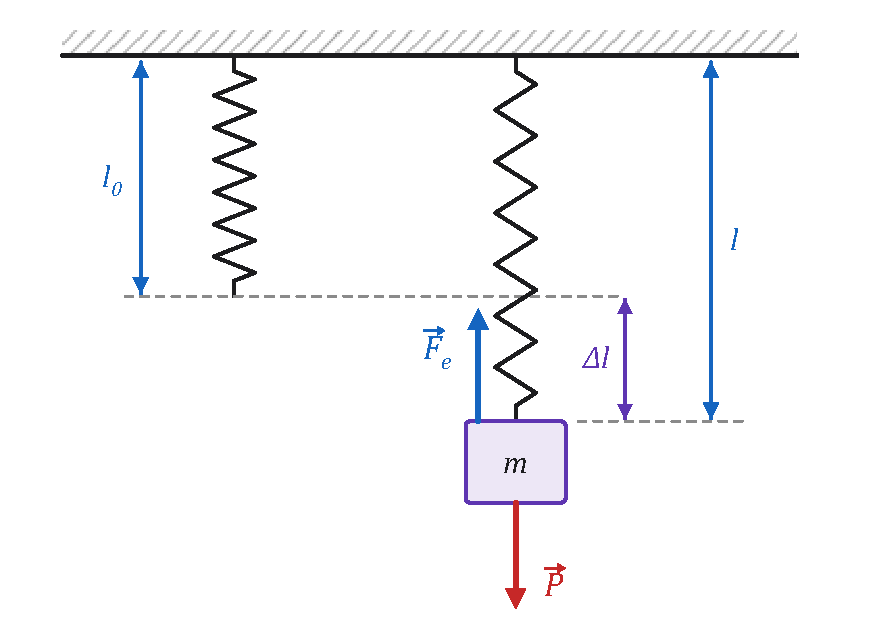
\includegraphics[width=0.55\linewidth]{images/UD1/muelle_hooke}
    \caption{Al colgar la masa, el muelle se alarga \(\Delta l\) hasta que la fuerza elástica equilibra al peso.}
    \label{fig:mas-hooke}
\end{figure}

Sobre el cuerpo actúan su peso y la fuerza elástica del muelle, que según la \rojon{ley de Hooke} es proporcional al
alargamiento, \(F_e = k\,\Delta l\). En el equilibrio:
\begin{equation*}
    \sum\vec F = 0 \;\Rightarrow\; P = F_e \;\Rightarrow\; m g = k\,(l - l_0) \;\Rightarrow\; \boxed{k = \dfrac{m g}{\Delta l}}
\end{equation*}
\(k\) es la \azuln{constante elástica} del muelle y se mide en \unit{\newton\per\m}: cuanto mayor es, más «duro» es el muelle.

\subsection{La fuerza recuperadora}\label{subsec:mas-recuperadora}

Si separamos el cuerpo de su posición de equilibrio y lo soltamos, el muelle ejerce una fuerza neta que tiende a devolverlo a
ella. Lo vemos más claro con un muelle horizontal sin rozamiento (figura~\ref{fig:mas-horizontal}):
\begin{itemize}
    \item si el cuerpo está a la derecha del equilibrio (\(x > 0\)), el muelle tira hacia la izquierda;
    \item si está a la izquierda (\(x < 0\)), lo empuja hacia la derecha;
    \item en la posición de equilibrio (\(x = 0\)) la fuerza es nula.
\end{itemize}

\begin{figure}[H]
    \centering
    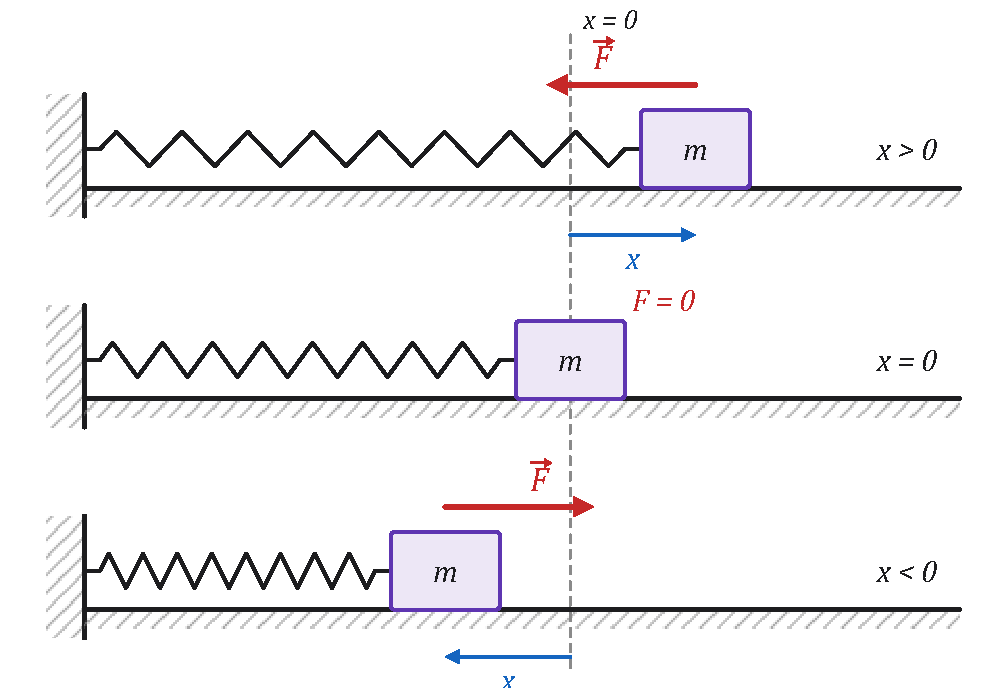
\includegraphics[width=0.72\linewidth]{images/UD1/muelle_horizontal}
    \caption{La fuerza del muelle es siempre opuesta al desplazamiento \(x\) respecto del equilibrio: \(F = -k\,x\).}
    \label{fig:mas-horizontal}
\end{figure}

Es exactamente la fuerza de la ecuación~\eqref{eq:mas-fuerza}, \(F = -k\,y\) (llamaremos \(y\) o \(x\) a la elongación según
la dirección del movimiento). En un muelle vertical ocurre lo mismo si medimos \(y\) desde la nueva posición de equilibrio
con la masa colgada: el peso queda compensado y la fuerza neta vuelve a ser \(-k\,y\).

Aplicando la segunda ley de Newton con la aceleración del m.a.s., \(a = -\omega^2 y\):
\begin{equation*}
    F = m\,a \;\Rightarrow\; -k\,y = -m\,\omega^2\,y \;\Rightarrow\; \boxed{k = m\,\omega^2}
\end{equation*}
y como \(\omega = 2\pi/T\):
\begin{centeredequation}
    \omega = \sqrt{\dfrac{k}{m}} \qquad\qquad \boxed{T = 2\pi\sqrt{\dfrac{m}{k}}} \label{eq:mas-periodo-muelle}
\end{centeredequation}

\begin{remark}
    El período de un oscilador depende solo de la masa y de la constante elástica, \textbf{no de la amplitud}: si lo
    separamos más, recorre más camino pero también va más deprisa, y tarda lo mismo. En los extremos la fuerza es máxima,
    \(F_{\text{máx}} = k\,A\).
\end{remark}

\begin{exercise}
    Si se triplica la masa que cuelga de un muelle, ¿cómo cambia la frecuencia de oscilación?
    \begin{solu}
        \textcolor{blue}{\(\nu = \dfrac{1}{T} = \dfrac{1}{2\pi}\sqrt{\dfrac{k}{m}}\). Con el mismo muelle (\(k\) igual):}
        \[ \dfrac{\nu_2}{\nu_1} = \sqrt{\dfrac{m_1}{m_2}} = \sqrt{\dfrac{m_1}{3m_1}} = \dfrac{1}{\sqrt 3} \;\Rightarrow\; \textcolor{red}{\nu_2 \approx 0{,}58\,\nu_1} \]
        \textcolor{red}{La frecuencia se divide por \(\sqrt 3\) (el muelle oscila más despacio).}
    \end{solu}
\end{exercise}

\begin{exercise}
    Un muelle mide \qty{30}{\cm} cuando cuelga de él una masa de \qty{200}{\g}. Si se añaden \qty{300}{\g} más, mide
    \qty{36}{\cm}. Calcula la constante elástica y la longitud del muelle sin carga.
    \begin{solu}
        \textcolor{blue}{La masa añadida (\qty{0.3}{\kg}) produce un alargamiento adicional de \qty{0.06}{\m}:}
        \[ k = \dfrac{\Delta m\,g}{\Delta l} = \dfrac{0{,}3\cdot 9{,}8}{0{,}06} = \textcolor{red}{\qty{49}{\newton\per\m}} \]
        \textcolor{blue}{Con \qty{0.2}{\kg}: \(0{,}2\cdot 9{,}8 = 49\,(0{,}30 - l_0) \Rightarrow 0{,}30 - l_0 = 0{,}04\)}
        \(\Rightarrow \textcolor{red}{l_0 = \qty{0.26}{\m} = \qty{26}{\cm}}\).
    \end{solu}
\end{exercise}

\begin{exercise}
    Un muelle se alarga \qty{5}{\cm} cuando se cuelga de él un cuerpo de \qty{10}{\kg}. Después se estira \qty{2}{\cm} más
    hacia abajo y se suelta. Tomando como positivo el sentido hacia arriba:
    \begin{enumerate}[label=\letraminuscula]
        \item Calcula la pulsación y el período.
        \item Escribe la ecuación del movimiento.
        \item Calcula la elongación, la velocidad, la aceleración y la fuerza recuperadora en \(t = \qty{1.5}{\second}\).
    \end{enumerate}
    \begin{solu}
        \begin{enumerate}[label=\letraminuscula]
            \item \textcolor{blue}{\(k = \dfrac{mg}{\Delta l} = \dfrac{10\cdot 9{,}8}{0{,}05} = \qty{1960}{\newton\per\m}\);}
            \(\omega = \sqrt{\dfrac{k}{m}} = \sqrt{196} = \textcolor{red}{\qty{14}{\radian\per\second}}\);
            \(T = \dfrac{2\pi}{\omega} = \textcolor{red}{\qty{0.449}{\second}}\).
            \item \textcolor{blue}{\(A = \qty{0.02}{\m}\) y en \(t = 0\) está en \(y = -A\): \(\sen\varphi_0 = -1 \Rightarrow \varphi_0 = 3\pi/2\).}
            \(\textcolor{red}{y = 0{,}02\,\sen\!\left(14 t + \dfrac{3\pi}{2}\right)\ \text{(m)}}\)
            \item \textcolor{blue}{En \(t = \qty{1.5}{\second}\) la fase vale \(14\cdot 1{,}5 + 3\pi/2 = \qty{25.71}{\radian}\) (calculadora en RAD):}
            \begin{itemize}
                \item \(y = 0{,}02\,\sen(25{,}71) = \textcolor{red}{\qty{1.10e-2}{\m}}\)
                \item \(v = 0{,}02\cdot 14\cos(25{,}71) = \textcolor{red}{\qty{0.234}{\m\per\second}}\)
                \item \(a = -\omega^2 y = -196\cdot 1{,}10\cdot 10^{-2} = \textcolor{red}{\qty{-2.15}{\m\per\second\squared}}\)
                \item \(F = -k\,y = -1960\cdot 1{,}10\cdot 10^{-2} = \textcolor{red}{\qty{-21.5}{\newton}}\)
            \end{itemize}
        \end{enumerate}
    \end{solu}
\end{exercise}

\begin{exercise}
    Un muelle de constante \qty{40}{\newton\per\m} mide \qty{25}{\cm} cuando cuelga de él una masa de \qty{0.4}{\kg}.
    \begin{enumerate}[label=\letraminuscula]
        \item ¿Cuánto mide sin carga?
        \item ¿Cuánto medirá si a la masa anterior se le añade otra de \qty{1.5}{\kg}?
    \end{enumerate}
    \begin{solu}
        \begin{enumerate}[label=\letraminuscula]
            \item \(\Delta l = \dfrac{mg}{k} = \dfrac{0{,}4\cdot 9{,}8}{40} = \qty{0.098}{\m}\);
            \(l_0 = 0{,}25 - 0{,}098 = \textcolor{red}{\qty{0.152}{\m} = \qty{15.2}{\cm}}\).
            \item \(\Delta l = \dfrac{1{,}9\cdot 9{,}8}{40} = \qty{0.466}{\m}\);
            \(l = 0{,}152 + 0{,}466 = \textcolor{red}{\qty{0.618}{\m} = \qty{61.8}{\cm}}\).
        \end{enumerate}
    \end{solu}
\end{exercise}

\section{El péndulo simple}\label{sec:mas-pendulo}

Un \rojon{péndulo simple} es una masa pequeña colgada de un hilo inextensible y de masa despreciable. En reposo, el peso y la
tensión del hilo se equilibran (\(\vec P + \vec T = 0\)). Si lo separamos un ángulo \(\varphi\), el peso se descompone en dos
partes (figura~\ref{fig:mas-pendulo}):
\begin{itemize}
    \item \(m g\cos\varphi\), en la dirección del hilo, que queda compensada por la tensión;
    \item \(m g\sen\varphi\), tangente a la trayectoria, que es la que mueve el péndulo hacia la posición de equilibrio:
\end{itemize}
\begin{centeredequation}
    F = -\,m g \sen\varphi \label{eq:mas-pendulo-fuerza}
\end{centeredequation}

\begin{figure}[H]
    \centering
    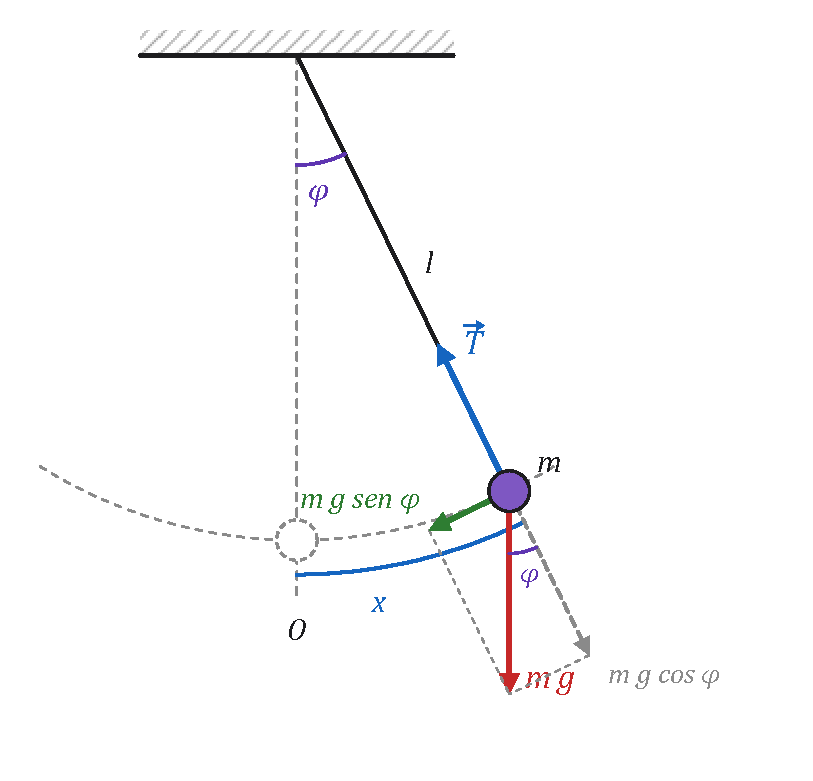
\includegraphics[width=0.5\linewidth]{images/UD1/pendulo}
    \caption{Fuerzas sobre un péndulo simple. La componente tangencial del peso, \(m g \sen\varphi\), lo devuelve hacia \(O\).}
    \label{fig:mas-pendulo}
\end{figure}

Esta fuerza no es exactamente proporcional al desplazamiento, así que en general el péndulo \emph{no} hace un m.a.s. Pero
para ángulos pequeños (menos de unos \ang{10}) se cumple \(\sen\varphi \approx \varphi\) (en radianes), y el arco recorrido es
\(x = l\,\varphi\). Entonces:
\begin{equation*}
    F \approx -\,m g\,\varphi = -\,\dfrac{m g}{l}\,x
\end{equation*}
que tiene la forma \(F = -k\,x\) con \(k = \dfrac{m g}{l}\). Igualando con \(k = m\omega^2\):
\begin{equation*}
    m\,\omega^2 = \dfrac{m g}{l} \;\Rightarrow\; \omega^2 = \dfrac{g}{l} \;\Rightarrow\; \dfrac{4\pi^2}{T^2} = \dfrac{g}{l}
\end{equation*}
\begin{centeredequation}
    \boxed{T = 2\pi\sqrt{\dfrac{l}{g}}} \label{eq:mas-periodo-pendulo}
\end{centeredequation}

\begin{remark}
    Para oscilaciones pequeñas, el período de un péndulo depende solo de su longitud y del valor de \(g\): \textbf{no depende
    de la masa ni de la amplitud} (isocronismo). Es proporcional a \(\sqrt l\) e inversamente proporcional a \(\sqrt g\), por
    eso un péndulo permite medir la gravedad (práctica~\ref{subsec:mas-practica-pendulo}).
\end{remark}

\begin{exercise}
    Comprueba con la calculadora la aproximación \(\sen\varphi \approx \varphi\) para \ang{2}, \ang{5}, \ang{10}, \ang{15} y
    \ang{20}. ¿Qué error relativo se comete en cada caso?
    \begin{solu}
        \textcolor{blue}{Pasamos cada ángulo a radianes y comparamos con su seno; error \(= (\varphi - \sen\varphi)/\sen\varphi\):}
        \begin{center}
            \begin{tabular}{@{}cccc@{}}
                \toprule
                \textbf{Ángulo} & \(\varphi\) (\unit{\radian}) & \(\sen\varphi\) & \textbf{Error} \\
                \midrule
                \ang{2} & \num{0.0349} & \num{0.0349} & \qty{0.02}{\percent} \\[3pt]
                \ang{5} & \num{0.0873} & \num{0.0872} & \qty{0.13}{\percent} \\[3pt]
                \ang{10} & \num{0.1745} & \num{0.1736} & \qty{0.51}{\percent} \\[3pt]
                \ang{15} & \num{0.2618} & \num{0.2588} & \qty{1.15}{\percent} \\[3pt]
                \ang{20} & \num{0.3491} & \num{0.3420} & \qty{2.06}{\percent} \\
                \bottomrule
            \end{tabular}
        \end{center}
        \textcolor{red}{Hasta \ang{10} el error no llega al \qty{0.5}{\percent}: la aproximación es muy buena.}
    \end{solu}
\end{exercise}

\begin{exercise}
    Un péndulo simple es cuatro veces más largo que otro. ¿Qué relación hay entre sus períodos?
    \begin{solu}
        \[ \dfrac{T_1}{T_2} = \dfrac{2\pi\sqrt{l_1/g}}{2\pi\sqrt{l_2/g}} = \sqrt{\dfrac{l_1}{l_2}} = \sqrt 4 = 2 \;\Rightarrow\; \textcolor{red}{T_1 = 2\,T_2} \]
    \end{solu}
\end{exercise}

\begin{exercise}
    Un reloj de péndulo bate segundos (\(T = \qty{2}{\second}\)) en un lugar donde \(g = \qty{9.81}{\m\per\second\squared}\).
    Lo llevamos a otro lugar donde \(g = \qty{9.78}{\m\per\second\squared}\).
    \begin{enumerate}[label=\letraminuscula]
        \item ¿Cuál será su nuevo período?
        \item ¿Cuánto se atrasará o adelantará en un día?
    \end{enumerate}
    \begin{solu}
        \begin{enumerate}[label=\letraminuscula]
            \item \textcolor{blue}{La longitud no cambia: \(\dfrac{T'}{T} = \sqrt{\dfrac{g}{g'}}\).}
            \(T' = 2\sqrt{\dfrac{9{,}81}{9{,}78}} = \textcolor{red}{\qty{2.0031}{\second}}\).
            \item \textcolor{blue}{En un día (\qty{86400}{\second}) da \(86400/2{,}0031 = \num{43134}\) oscilaciones, y el reloj cuenta
            \qty{2}{\second} por cada una: marca \(\qty{86268}{\second}\).}
            \textcolor{red}{Se atrasa unos \qty{132}{\second} (algo más de 2 minutos) al día.}
        \end{enumerate}
    \end{solu}
\end{exercise}

\section{Energía del movimiento armónico simple}\label{sec:mas-energia}

Un oscilador tiene dos tipos de energía: \textbf{cinética}, por su velocidad, y \textbf{potencial elástica}, asociada a la
fuerza recuperadora.

\paragraph{Energía cinética.} Con \(v = A\omega\cos(\omega t + \varphi_0)\) y \(k = m\omega^2\):
\begin{equation*}
    E_c = \dfrac{1}{2} m v^2 = \dfrac{1}{2} m A^2\omega^2\cos^2(\omega t + \varphi_0) = \dfrac{1}{2} k A^2\left[1 - \sen^2(\omega t + \varphi_0)\right]
    \;\Rightarrow\; \boxed{E_c = \dfrac{1}{2} k\,(A^2 - y^2)}
\end{equation*}
Es máxima en el centro (\(y = 0\)) y nula en los extremos (\(y = \pm A\)).

\paragraph{Energía potencial elástica.} La fuerza recuperadora es conservativa; su trabajo es igual a menos la variación de
energía potencial. Tomando \(E_p = 0\) en \(y = 0\):
\begin{equation*}
    W_{F_e} = -\Delta E_p \;\Rightarrow\; E_p = -\int_0^y (-k\,y)\,dy = k\left[\dfrac{y^2}{2}\right]_0^y \;\Rightarrow\; \boxed{E_p = \dfrac{1}{2} k\,y^2}
\end{equation*}
Es nula en el centro y máxima en los extremos.

\paragraph{Energía mecánica.} Sumando ambas:
\begin{centeredequation}
    E_m = E_c + E_p = \dfrac{1}{2}k(A^2 - y^2) + \dfrac{1}{2}k y^2 = \boxed{\dfrac{1}{2} k A^2} = \dfrac{1}{2} m\omega^2 A^2 = 2\pi^2 m \nu^2 A^2 \label{eq:mas-energia}
\end{centeredequation}

\begin{remark}
    Si no hay rozamiento, la energía mecánica de un oscilador \textbf{se conserva} y es proporcional al cuadrado de la
    amplitud (y al cuadrado de la frecuencia). Durante la oscilación la energía pasa continuamente de potencial (extremos) a
    cinética (centro) y al revés (figura~\ref{fig:mas-energia}).
\end{remark}

\begin{figure}[H]
    \centering
    \begin{tikzpicture}
        \begin{axis}[fisica, width=0.62\linewidth, height=5.6cm, xmin=-1.25, xmax=1.3, ymin=0, ymax=1.3,
            xlabel={\(y\)}, ylabel={\(E\)}, xtick={-1,1}, xticklabels={\(-A\),\(A\)},
            ytick={1}, yticklabels={\(\frac{1}{2}kA^2\)}, legend style={font=\small, at={(1.02,0.62)}, anchor=west, draw=none}]
            \addplot[domain=-1:1, very thick, red] {x^2};
            \addlegendentry{\(E_p = \frac{1}{2}k y^2\)}
            \addplot[domain=-1:1, very thick, blue] {1-x^2};
            \addlegendentry{\(E_c = \frac{1}{2}k(A^2-y^2)\)}
            \addplot[domain=-1:1, very thick, ocre] {1};
            \addlegendentry{\(E_m\)}
            \draw[dashed, gray] (axis cs:0.55,0) -- (axis cs:0.55,1);
            \draw[<->, red, thick] (axis cs:0.62,0) -- node[right, font=\scriptsize]{\(E_p\)} (axis cs:0.62,0.3025);
            \draw[<->, blue, thick] (axis cs:0.62,0.3025) -- node[right, font=\scriptsize]{\(E_c\)} (axis cs:0.62,1);
        \end{axis}
    \end{tikzpicture}
    \caption{Energías de un oscilador en función de la elongación. En cualquier posición \(E_c + E_p = E_m\).}
    \label{fig:mas-energia}
\end{figure}

\begin{exercise}
    Un cuerpo de \qty{0.5}{\kg} unido a un muelle de \qty{200}{\newton\per\m} oscila con una amplitud de \qty{10}{\cm}.
    Calcula su energía mecánica y, cuando está a \qty{5}{\cm} del equilibrio, sus energías potencial y cinética y su velocidad.
    \begin{solu}
        \textcolor{blue}{\(E_m = \frac{1}{2}kA^2 = \frac{1}{2}\cdot 200\cdot 0{,}1^2\)} \(= \textcolor{red}{\qty{1}{\joule}}\).

        \textcolor{blue}{En \(y = \qty{0.05}{\m}\):} \(E_p = \frac{1}{2}\cdot 200\cdot 0{,}05^2 = \textcolor{red}{\qty{0.25}{\joule}}\);
        \(E_c = E_m - E_p = \textcolor{red}{\qty{0.75}{\joule}}\).

        \(v = \sqrt{\dfrac{2E_c}{m}} = \sqrt{\dfrac{2\cdot 0{,}75}{0{,}5}} = \textcolor{red}{\qty{1.73}{\m\per\second}}\).
        \textcolor{blue}{(A mitad de la amplitud solo una cuarta parte de la energía es potencial.)}
    \end{solu}
\end{exercise}

\section{Resumen de fórmulas}\label{sec:mas-resumen}

\begin{table}[H]
    \centering
    \caption{Fórmulas principales del movimiento armónico simple}
    \vspace{-5pt}
    \begin{tabular}{@{}lll@{}}
        \toprule
        \textbf{Magnitud} & \textbf{Expresión} & \textbf{Valor máximo} \\
        \midrule
        Elongación & \(y = A\sen(\omega t + \varphi_0)\) & \(A\) \\[3pt]
        Velocidad & \(v = A\omega\cos(\omega t + \varphi_0) = \pm\,\omega\sqrt{A^2 - y^2}\) & \(A\omega\) (en el centro) \\[3pt]
        Aceleración & \(a = -A\omega^2\sen(\omega t + \varphi_0) = -\omega^2 y\) & \(A\omega^2\) (en los extremos) \\[3pt]
        Fuerza recuperadora & \(F = -k\,y\), \quad \(k = m\omega^2\) & \(kA\) \\[3pt]
        Período (muelle) & \(T = 2\pi\sqrt{m/k}\) & --- \\[3pt]
        Período (péndulo) & \(T = 2\pi\sqrt{l/g}\) \quad (ángulos pequeños) & --- \\[3pt]
        Energías & \(E_c = \frac{1}{2}k(A^2 - y^2)\), \quad \(E_p = \frac{1}{2}k y^2\) & \(E_m = \frac{1}{2}kA^2\) \\
        \bottomrule
    \end{tabular}
    \label{tab:mas-resumen}
\end{table}

\section{Prácticas de laboratorio}\label{sec:mas-practicas}

\subsection{Práctica 1: el oscilador armónico}\label{subsec:mas-practica-muelle}

\noindent\begin{minipage}[t]{0.64\linewidth}
\textbf{Objetivo.} Estudiar cómo depende el período de un muelle de la masa que cuelga de él y calcular su constante elástica.

\textbf{Material.} Soporte con varilla y pinza, muelle, portapesas, pesas de distintas masas, regla y cronómetro.

\textbf{Procedimiento.}
\begin{enumerate}[label=\numberballmDarkTeal]
    \item Monta el muelle en el soporte (figura~\ref{fig:mas-practica-muelle}) y cuelga el portapesas con una primera masa.
    \item Separa la masa un poco de su posición de equilibrio (unos \qty{2}{\cm}) y suéltala.
    \item Mide el tiempo de 10 oscilaciones completas. Repite la medida tres veces y calcula la media; el período es esa
    media dividida entre 10.
    \item Repite el proceso con al menos otras tres masas distintas y anota los datos en la tabla.
\end{enumerate}
\end{minipage}\hfill
\begin{minipage}[t]{0.32\linewidth}
    \vspace{0pt}
    \centering
    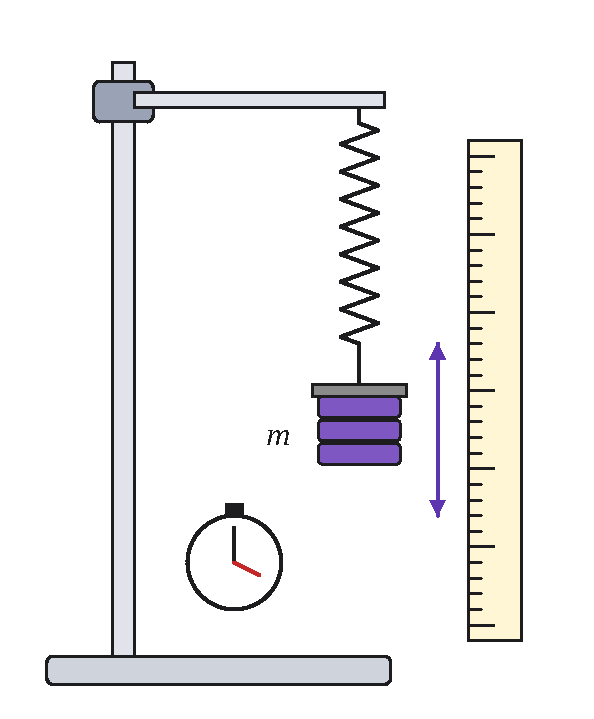
\includegraphics[width=0.9\linewidth]{images/UD1/practica_muelle}
    \captionof{figure}{Montaje de la práctica.}
    \label{fig:mas-practica-muelle}
\end{minipage}

\begin{table}[H]
    \centering
    \caption{Datos de la práctica del oscilador}
    \vspace{-5pt}
    \begin{tabular}{@{}C{2.2cm}C{3.4cm}C{2.2cm}C{2.2cm}C{2.6cm}@{}}
        \toprule
        \textbf{\(m\) (\unit{\kg})} & \textbf{Tiempo de 10 oscilaciones (\unit{\second})} & \textbf{\(T\) (\unit{\second})} & \textbf{\(T^2\) (\unit{\second\squared})} & \textbf{\(k\) (\unit{\newton\per\m})} \\
        \midrule
        \rule{0pt}{18pt} & & & & \\ \midrule[0.3pt]
        \rule{0pt}{18pt} & & & & \\ \midrule[0.3pt]
        \rule{0pt}{18pt} & & & & \\ \midrule[0.3pt]
        \rule{0pt}{18pt} & & & & \\
        \bottomrule
    \end{tabular}
    \label{tab:mas-practica-muelle}
\end{table}

\textbf{Cálculos.} De \(k = m\omega^2\) y \(\omega = 2\pi/T\) se obtiene:
\begin{equation*}
    T^2 = \dfrac{4\pi^2}{k}\,m
\end{equation*}
Con cada pareja \((m, T)\) calcula \(k = 4\pi^2 m / T^2\) y halla el valor medio.

\textbf{Método gráfico.} Representa \(T^2\) frente a \(m\). Los puntos deben quedar sobre una recta que pasa (casi) por el
origen, \(T^2 = b\,m\), cuya pendiente es \(b = 4\pi^2/k\). Traza la recta que mejor se ajuste y calcula \(k = 4\pi^2/b\).

\textbf{Cuestiones.}
\begin{enumerate}[label=\letraminuscula]
    \item ¿Por qué se mide el tiempo de 10 oscilaciones en lugar de una sola?
    \item Compara el valor de \(k\) obtenido con el cálculo directo y con la gráfica. ¿Cuál te parece más fiable y por qué?
    \item Cuelga una masa y mide el alargamiento \(\Delta l\). Calcula \(k = mg/\Delta l\) y compáralo con el obtenido.
\end{enumerate}

\subsection{Práctica 2: medida de \texorpdfstring{\(g\)}{g} con un péndulo simple}\label{subsec:mas-practica-pendulo}

\noindent\begin{minipage}[t]{0.64\linewidth}
\textbf{Objetivo.} Medir la aceleración de la gravedad con un péndulo simple y comprobar que, para oscilaciones pequeñas, su
período no depende de la amplitud ni de la masa.

\textbf{Material.} Soporte, doble nuez, varilla, hilo con una bola pequeña, regla graduada y cronómetro.

\textbf{Procedimiento.}
\begin{enumerate}[label=\numberballmDarkTeal]
    \item Monta el péndulo (figura~\ref{fig:mas-practica-pendulo}) y mide su longitud \(l\) desde el punto de suspensión
    hasta el centro de la bola.
    \item Sepáralo un ángulo pequeño (menos de \ang{10}) y suéltalo, cuidando de que oscile en un plano y no describa elipses.
    \item Mide el tiempo de 10 oscilaciones, repite la medida varias veces y calcula el período medio.
    \item Repite con otras longitudes. Para comprobar el isocronismo, repite una medida con otra amplitud (siempre pequeña)
    y con otra bola de distinta masa.
\end{enumerate}
\end{minipage}\hfill
\begin{minipage}[t]{0.32\linewidth}
    \vspace{0pt}
    \centering
    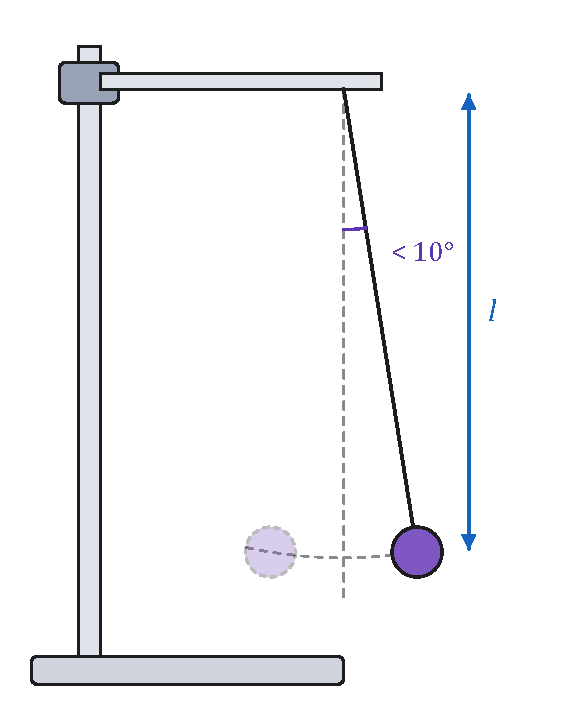
\includegraphics[width=0.9\linewidth]{images/UD1/practica_pendulo}
    \captionof{figure}{Montaje de la práctica.}
    \label{fig:mas-practica-pendulo}
\end{minipage}

\begin{table}[H]
    \centering
    \caption{Datos de la práctica del péndulo}
    \vspace{-5pt}
    \begin{tabular}{@{}C{2.6cm}C{3.6cm}C{2.4cm}C{2.4cm}C{2.4cm}@{}}
        \toprule
        \textbf{\(l\) (\unit{\m})} & \textbf{Tiempo de 10 oscilaciones (\unit{\second})} & \textbf{\(T\) (\unit{\second})} & \textbf{\(T^2\) (\unit{\second\squared})} & \textbf{\(g\) (\unit{\m\per\second\squared})} \\
        \midrule
        \rule{0pt}{18pt} & & & & \\ \midrule[0.3pt]
        \rule{0pt}{18pt} & & & & \\ \midrule[0.3pt]
        \rule{0pt}{18pt} & & & & \\ \midrule[0.3pt]
        \rule{0pt}{18pt} & & & & \\
        \bottomrule
    \end{tabular}
    \label{tab:mas-practica-pendulo}
\end{table}

\textbf{Cálculos.} De \(T = 2\pi\sqrt{l/g}\) se despeja \(g = \dfrac{4\pi^2 l}{T^2}\) para cada longitud.

\textbf{Método gráfico.} Representa \(T^2\) frente a \(l\): \(T^2 = \dfrac{4\pi^2}{g}\,l\) es una recta del tipo \(y = m x\)
con pendiente \(m = 4\pi^2/g\). Ajusta la recta y calcula \(g = 4\pi^2/m\).

\textbf{Cuestiones.}
\begin{enumerate}[label=\letraminuscula]
    \item ¿Has observado que el período cambie al usar otra bola o al soltar el péndulo desde otro ángulo pequeño?
    \item Calcula el error relativo de tu medida tomando como valor de referencia \(g = \qty{9.80}{\m\per\second\squared}\).
    \item ¿Qué ocurriría con el período si soltaras el péndulo desde \ang{45}? Justifícalo con la aproximación \(\sen\varphi \approx \varphi\).
\end{enumerate}


    \newpage

    %! Unidad 1 — Movimiento armónico simple: ejercicios finales (adaptados de la fuente, con datos cambiados y resueltos)

\section{Ejercicios}\label{sec:mas-ejercicios}

\subsection{Cinemática del m.a.s.}

\begin{exercise}
    Una partícula oscila con un m.a.s. cuya aceleración máxima es \qty{20}{\m\per\second\squared} y cuya velocidad máxima
    es \qty{4}{\m\per\second}. Calcula:
    \begin{enumerate}[label=\letraminuscula]
        \item La frecuencia de oscilación.
        \item La amplitud del movimiento.
    \end{enumerate}
    \begin{solu}
        \textcolor{blue}{\(a_{\text{máx}} = A\omega^2\) y \(v_{\text{máx}} = A\omega\); dividiendo: \(\omega = \dfrac{a_{\text{máx}}}{v_{\text{máx}}} = \dfrac{20}{4} = \qty{5}{\radian\per\second}\).}
        \begin{enumerate}[label=\letraminuscula]
            \item \(\nu = \dfrac{\omega}{2\pi} = \textcolor{red}{\qty{0.80}{\hertz}}\).
            \item \(A = \dfrac{v_{\text{máx}}}{\omega} = \dfrac{4}{5} = \textcolor{red}{\qty{0.8}{\m}}\).
        \end{enumerate}
    \end{solu}
\end{exercise}

\begin{exercise}
    La ecuación de un m.a.s. es \(y = 4\,\sen\!\left(\dfrac{\pi}{2}\,t\right)\) en unidades del SI.
    \begin{enumerate}[label=\letraminuscula]
        \item ¿Cuáles son su período, su frecuencia y su amplitud?
        \item Si la masa del cuerpo es \qty{0.5}{\kg}, ¿cuál es su energía cinética en \(t = \qty{0.5}{\second}\)?
        \item ¿En qué instante alcanza por primera vez la separación máxima?
    \end{enumerate}
    \begin{solu}
        \begin{enumerate}[label=\letraminuscula]
            \item \textcolor{blue}{\(\omega = \pi/2\ \unit{\radian\per\second}\):} \(T = \dfrac{2\pi}{\omega} = \textcolor{red}{\qty{4}{\second}}\);
            \(\nu = \textcolor{red}{\qty{0.25}{\hertz}}\); \(A = \textcolor{red}{\qty{4}{\m}}\).
            \item \(v = A\omega\cos(\omega t) = 4\cdot\dfrac{\pi}{2}\cos\dfrac{\pi}{4} = \qty{4.44}{\m\per\second}\);
            \(E_c = \frac{1}{2}\cdot 0{,}5\cdot 4{,}44^2 = \textcolor{red}{\qty{4.93}{\joule}}\).
            \item \textcolor{blue}{\(y = A\) cuando \(\sen(\pi t/2) = 1 \Rightarrow \pi t/2 = \pi/2\)} \(\Rightarrow \textcolor{red}{t = \qty{1}{\second}}\) (un cuarto de período).
        \end{enumerate}
    \end{solu}
\end{exercise}

\begin{exercise}
    Un m.a.s. tiene un período de \qty{4}{\second} y una amplitud de \qty{5}{\cm}. El móvil pasa por el centro de la
    trayectoria, moviéndose en sentido positivo, en \(t = \qty{2}{\second}\). Escribe la ecuación del movimiento y calcula la
    velocidad en \(t = \qty{4}{\second}\).
    \begin{solu}
        \textcolor{blue}{\(\omega = \dfrac{2\pi}{4} = \dfrac{\pi}{2}\ \unit{\radian\per\second}\), \(A = \qty{0.05}{\m}\). En \(t = 2\): \(y = 0\) y \(v > 0\), luego la fase
        vale \(0\) (o \(2\pi\)): \(\dfrac{\pi}{2}\cdot 2 + \varphi_0 = 2\pi \Rightarrow \varphi_0 = \pi\).}
        \[ \textcolor{red}{y = 0{,}05\,\sen\!\left(\dfrac{\pi}{2}t + \pi\right)\ \text{(m)}} \]
        \(v(4) = 0{,}05\cdot\dfrac{\pi}{2}\cos(2\pi + \pi) = \textcolor{red}{\qty{-0.0785}{\m\per\second}}\) \textcolor{blue}{(vuelve a pasar por el centro, ahora hacia abajo).}
    \end{solu}
\end{exercise}

\begin{exercise}
    Escribe la ecuación de un m.a.s. de amplitud \qty{10}{\cm} y frecuencia \qty{2}{\hertz} sabiendo que en \(t = 0\) el móvil
    está en el punto medio de la amplitud positiva (\(y = A/2\)) y se aleja del centro.
    \begin{solu}
        \textcolor{blue}{\(\omega = 2\pi\nu = 4\pi\ \unit{\radian\per\second}\). En \(t = 0\): \(\sen\varphi_0 = \dfrac{1}{2}\); como se aleja del centro, \(v > 0\) y
        \(\cos\varphi_0 > 0\), así que \(\varphi_0 = \dfrac{\pi}{6}\) (la otra solución, \(5\pi/6\), corresponde a acercarse).}
        \[ \textcolor{red}{y = 0{,}10\,\sen\!\left(4\pi t + \dfrac{\pi}{6}\right)\ \text{(m)}} \]
    \end{solu}
\end{exercise}

\begin{exercise}
    Un punto vibra con una amplitud de \qty{3}{\cm} y una frecuencia de \qty{60}{\hertz}. Calcula:
    \begin{enumerate}[label=\letraminuscula]
        \item La velocidad máxima.
        \item La velocidad cuando la elongación es de \qty{1}{\cm}.
        \item Cuántas vibraciones da en un minuto.
    \end{enumerate}
    \begin{solu}
        \textcolor{blue}{\(\omega = 2\pi\cdot 60 = 120\pi\ \unit{\radian\per\second}\).}
        \begin{enumerate}[label=\letraminuscula]
            \item \(v_{\text{máx}} = A\omega = 0{,}03\cdot 120\pi = \textcolor{red}{\qty{11.3}{\m\per\second}}\).
            \item \(v = \omega\sqrt{A^2 - y^2} = 120\pi\sqrt{0{,}03^2 - 0{,}01^2} = \textcolor{red}{\qty{10.7}{\m\per\second}}\).
            \item \(60\ \unit{\hertz}\cdot\qty{60}{\second} = \textcolor{red}{\num{3600}\ \text{vibraciones}}\).
        \end{enumerate}
    \end{solu}
\end{exercise}

\begin{exercise}
    Una partícula tiene un m.a.s. de período \qty{6}{\second} y fase inicial nula. Calcula:
    \begin{enumerate}[label=\letraminuscula]
        \item El tiempo que tarda en tener una velocidad igual a la mitad de la máxima.
        \item El instante en que la elongación es la mitad de la amplitud.
    \end{enumerate}
    \begin{solu}
        \textcolor{blue}{\(\omega = 2\pi/6 = \pi/3\ \unit{\radian\per\second}\).}
        \begin{enumerate}[label=\letraminuscula]
            \item \(A\omega\cos\omega t = \dfrac{A\omega}{2} \Rightarrow \cos\omega t = \dfrac{1}{2} \Rightarrow \omega t = \dfrac{\pi}{3}\)
            \(\Rightarrow \textcolor{red}{t = \qty{1}{\second}} = T/6\).
            \item \(A\sen\omega t = \dfrac{A}{2} \Rightarrow \omega t = \dfrac{\pi}{6}\) \(\Rightarrow \textcolor{red}{t = \qty{0.5}{\second}} = T/12\).
        \end{enumerate}
        \textcolor{blue}{Fíjate en que no tarda \(T/8\) en llegar a \(A/2\): al principio va más deprisa.}
    \end{solu}
\end{exercise}

\begin{exercise}
    ¿Cómo cambian la velocidad máxima y la aceleración máxima de un m.a.s. si:
    \begin{enumerate}[label=\letraminuscula]
        \item se triplica la frecuencia y se reduce la amplitud a la mitad?
        \item se reduce la frecuencia a la mitad manteniendo la amplitud?
    \end{enumerate}
    \begin{solu}
        \textcolor{blue}{\(v_{\text{máx}} = A\omega = 2\pi\nu A\) y \(a_{\text{máx}} = A\omega^2 = 4\pi^2\nu^2 A\).}
        \begin{enumerate}[label=\letraminuscula]
            \item \(v'_{\text{máx}} \propto 3\nu\cdot\dfrac{A}{2}\): \textcolor{red}{se multiplica por \(1{,}5\)}; \(a'_{\text{máx}} \propto 9\nu^2\cdot\dfrac{A}{2}\): \textcolor{red}{se multiplica por \(4{,}5\)}.
            \item \textcolor{red}{\(v_{\text{máx}}\) se reduce a la mitad y \(a_{\text{máx}}\) a la cuarta parte.}
        \end{enumerate}
    \end{solu}
\end{exercise}

\begin{exercise}
    Una partícula con m.a.s. recorre \qty{20}{\cm} en cada ciclo y su aceleración máxima es \qty{20}{\m\per\second\squared}.
    Calcula la frecuencia, el período y la velocidad máxima.
    \begin{solu}
        \textcolor{blue}{En un ciclo recorre \(4A\): \(A = \qty{0.05}{\m}\). \(\omega = \sqrt{\dfrac{a_{\text{máx}}}{A}} = \sqrt{\dfrac{20}{0{,}05}} = \qty{20}{\radian\per\second}\).}

        \(\nu = \dfrac{20}{2\pi} = \textcolor{red}{\qty{3.18}{\hertz}}\); \(T = \textcolor{red}{\qty{0.314}{\second}}\);
        \(v_{\text{máx}} = A\omega = \textcolor{red}{\qty{1}{\m\per\second}}\).
    \end{solu}
\end{exercise}

\begin{exercise}
    Una partícula con m.a.s. recorre \qty{24}{\cm} en cada ciclo y su aceleración máxima es \qty{54}{\cm\per\second\squared}.
    Calcula la frecuencia, el período y la velocidad máxima.
    \begin{solu}
        \textcolor{blue}{\(4A = \qty{24}{\cm} \Rightarrow A = \qty{0.06}{\m}\); \(\omega = \sqrt{\dfrac{0{,}54}{0{,}06}} = \qty{3}{\radian\per\second}\).}

        \(\nu = \textcolor{red}{\qty{0.477}{\hertz}}\); \(T = \dfrac{2\pi}{3} = \textcolor{red}{\qty{2.09}{\second}}\);
        \(v_{\text{máx}} = 0{,}06\cdot 3 = \textcolor{red}{\qty{0.18}{\m\per\second}}\).
    \end{solu}
\end{exercise}

\begin{exercise}
    Deduce la ecuación de la elongación de los movimientos representados en las gráficas (en todas, el tiempo está en
    segundos):

    \begin{center}
        \begin{tikzpicture}
            \begin{axis}[fisica, width=0.46\linewidth, xmin=0, xmax=0.48, ymin=-5.5, ymax=5.8, xlabel={\(t\)}, ylabel={(a) \(y\) (\unit{\cm})},
                xtick={0.1,0.2,0.3,0.4}, xticklabel style={/pgf/number format/use comma}, ytick={-4,4}]
                \addplot[domain=0:0.45, very thick, ocre] {4*sin(deg(5*pi*x))};
            \end{axis}
        \end{tikzpicture}\hfill
        \begin{tikzpicture}
            \begin{axis}[fisica, width=0.46\linewidth, xmin=0, xmax=0.48, ymin=-7.5, ymax=7.8, xlabel={\(t\)}, ylabel={(b) \(y\) (\unit{\cm})},
                xtick={0.1,0.2,0.3,0.4}, xticklabel style={/pgf/number format/use comma}, ytick={-6,6}]
                \addplot[domain=0:0.45, very thick, ocre] {6*cos(deg(5*pi*x))};
            \end{axis}
        \end{tikzpicture}

        \vspace{6pt}
        \begin{tikzpicture}
            \begin{axis}[fisica, width=0.46\linewidth, xmin=0, xmax=0.24, ymin=-190, ymax=200, xlabel={\(t\)}, ylabel={(c) \(v\) (\unit{\cm\per\second})},
                xtick={0.05,0.1,0.15,0.2}, xticklabel style={/pgf/number format/use comma}, ytick={-150,150}]
                \addplot[domain=0:0.225, very thick, blue] {-150*sin(deg(10*pi*x))};
            \end{axis}
        \end{tikzpicture}\hfill
        \begin{tikzpicture}
            \begin{axis}[fisica, width=0.46\linewidth, xmin=0, xmax=0.48, ymin=-500, ymax=520, xlabel={\(t\)}, ylabel={(d) \(a\) (\unit{\cm\per\second\squared})},
                xtick={0.1,0.2,0.3,0.4}, xticklabel style={/pgf/number format/use comma}, ytick={-400,400}]
                \addplot[domain=0:0.45, very thick, red] {400*sin(deg(5*pi*x))};
            \end{axis}
        \end{tikzpicture}
    \end{center}
    \begin{solu}
        \begin{enumerate}[label=\letraminuscula]
            \item \textcolor{blue}{\(A = \qty{0.04}{\m}\), \(T = \qty{0.4}{\second} \Rightarrow \omega = 5\pi\ \unit{\radian\per\second}\); empieza en \(y = 0\) subiendo: \(\varphi_0 = 0\).}
            \(\textcolor{red}{y = 0{,}04\,\sen(5\pi t)\ \text{(m)}}\)
            \item \textcolor{blue}{\(A = \qty{0.06}{\m}\), \(\omega = 5\pi\); empieza en el extremo positivo: \(\varphi_0 = \pi/2\).}
            \(\textcolor{red}{y = 0{,}06\,\sen\!\left(5\pi t + \dfrac{\pi}{2}\right)\ \text{(m)}}\)
            \item \textcolor{blue}{\(T = \qty{0.2}{\second} \Rightarrow \omega = 10\pi\); \(A\omega = \qty{1.5}{\m\per\second} \Rightarrow A = \dfrac{1{,}5}{10\pi} = \qty{0.0477}{\m}\).
            En \(t = 0\), \(v = 0\) y empieza a ser negativa: está en el extremo positivo, \(\varphi_0 = \pi/2\).}
            \(\textcolor{red}{y = 0{,}0477\,\sen\!\left(10\pi t + \dfrac{\pi}{2}\right)\ \text{(m)}}\)
            \item \textcolor{blue}{\(\omega = 5\pi\); \(A\omega^2 = \qty{4}{\m\per\second\squared} \Rightarrow A = \dfrac{4}{25\pi^2} = \qty{0.0162}{\m}\).
            Como \(a = -\omega^2 y\), si la aceleración empieza en 0 creciendo, la posición empieza en 0 decreciendo: \(\varphi_0 = \pi\).}
            \(\textcolor{red}{y = 0{,}0162\,\sen(5\pi t + \pi)\ \text{(m)}}\)
        \end{enumerate}
    \end{solu}
\end{exercise}

\subsection{Dinámica del m.a.s.: muelles y péndulos}

\begin{exercise}
    Un cuerpo de \qty{50}{\kg} oscila sobre una superficie horizontal sin rozamiento unido a un muelle, con una frecuencia de
    \qty{3}{\hertz} y una amplitud de \qty{8}{\cm}. ¿Cuánto vale la constante del muelle?
    \begin{solu}
        \textcolor{blue}{\(k = m\omega^2 = m\,(2\pi\nu)^2 = 50\cdot(6\pi)^2 = 1800\pi^2\)} \(= \textcolor{red}{\qty{1.78e4}{\newton\per\m}}\).
        \textcolor{blue}{(La amplitud no influye en \(k\).)}
    \end{solu}
\end{exercise}

\begin{exercise}
    Un punto material de \qty{40}{\g} describe un m.a.s. de \qty{12}{\cm} de amplitud y \qty{2}{\second} de período. En
    \(t = 0\) su elongación es máxima. Calcula:
    \begin{enumerate}[label=\letraminuscula]
        \item La velocidad máxima.
        \item La fuerza recuperadora en \(t = \qty{0.25}{\second}\).
    \end{enumerate}
    \begin{solu}
        \textcolor{blue}{\(\omega = \pi\ \unit{\radian\per\second}\), \(\varphi_0 = \pi/2\): \(y = 0{,}12\,\sen(\pi t + \pi/2)\).}
        \begin{enumerate}[label=\letraminuscula]
            \item \(v_{\text{máx}} = A\omega = 0{,}12\pi = \textcolor{red}{\qty{0.377}{\m\per\second}}\).
            \item \(y(0{,}25) = 0{,}12\,\sen(0{,}75\pi) = \qty{0.0849}{\m}\);
            \(F = -m\omega^2 y = -0{,}04\cdot\pi^2\cdot 0{,}0849 = \textcolor{red}{\qty{-0.0335}{\newton}}\).
        \end{enumerate}
    \end{solu}
\end{exercise}

\begin{exercise}
    La energía total de un cuerpo con m.a.s. es \qty{4e-4}{\joule} y la fuerza máxima que actúa sobre él es
    \qty{2e-2}{\newton}. Si el período es \qty{4}{\second} y la fase inicial \ang{30}, determina:
    \begin{enumerate}[label=\letraminuscula]
        \item La ecuación del movimiento.
        \item La velocidad y la aceleración en \(t = 0\).
    \end{enumerate}
    \begin{solu}
        \textcolor{blue}{\(E = \frac{1}{2}kA^2\) y \(F_{\text{máx}} = kA\); dividiendo: \(\dfrac{E}{F_{\text{máx}}} = \dfrac{A}{2}
        \Rightarrow A = \dfrac{2\cdot 4\cdot 10^{-4}}{2\cdot 10^{-2}} = \qty{0.04}{\m}\). \(\omega = 2\pi/4 = \pi/2\); \(\varphi_0 = \pi/6\).}
        \begin{enumerate}[label=\letraminuscula]
            \item \(\textcolor{red}{y = 0{,}04\,\sen\!\left(\dfrac{\pi}{2}t + \dfrac{\pi}{6}\right)\ \text{(m)}}\)
            \item \(v(0) = 0{,}04\cdot\dfrac{\pi}{2}\cos\dfrac{\pi}{6} = \textcolor{red}{\qty{0.0544}{\m\per\second}}\);
            \(a(0) = -0{,}04\cdot\dfrac{\pi^2}{4}\sen\dfrac{\pi}{6} = \textcolor{red}{\qty{-0.0493}{\m\per\second\squared}}\).
        \end{enumerate}
    \end{solu}
\end{exercise}

\begin{exercise}
    Para calibrar un muelle se cuelgan distintas masas y se mide su longitud:
    \begin{center}
        \begin{tabular}{@{}lcccccc@{}}
            \toprule
            \textbf{Masa (\unit{\g})} & 0 & 50 & 100 & 150 & 200 & 250 \\
            \midrule
            \textbf{Longitud (\unit{\mm})} & \num{60.0} & \num{64.9} & \num{69.8} & \num{74.8} & \num{79.6} & \num{84.5} \\
            \bottomrule
        \end{tabular}
    \end{center}
    Calcula la constante del muelle mediante una representación gráfica.
    \begin{solu}
        \textcolor{blue}{Representamos el peso \(F = mg\) frente al alargamiento \(\Delta l = l - l_0\). La pendiente es \(k\):}
        \begin{center}
            \begin{tikzpicture}
                \begin{axis}[fisica, width=0.55\linewidth, height=5cm, xmin=0, xmax=28, ymin=0, ymax=2.8,
                    xlabel={\(\Delta l\) (\unit{\mm})}, ylabel={\(F\) (\unit{\newton})}, yticklabel style={/pgf/number format/use comma}]
                    \addplot[only marks, mark=*, ocre] coordinates {(0,0) (4.9,0.49) (9.8,0.98) (14.8,1.47) (19.6,1.96) (24.5,2.45)};
                    \addplot[domain=0:26, thick, red] {0.09994*x};
                \end{axis}
            \end{tikzpicture}
        \end{center}
        \textcolor{blue}{La recta de ajuste pasa por \((24{,}5\ \unit{\mm};\ \qty{2.45}{\newton})\):}
        \(k = \dfrac{2{,}45}{0{,}0245} = \textcolor{red}{\qty{100}{\newton\per\m}}\) \textcolor{blue}{(longitud natural \qty{60}{\mm}).}
    \end{solu}
\end{exercise}

\begin{exercise}
    Un muelle de masa despreciable mide \qty{10}{\cm}; un extremo está fijo a una pared y el otro unido a una masa que
    descansa sobre una superficie horizontal sin rozamiento. Hace falta una fuerza de \qty{24}{\newton} para mantenerlo
    estirado hasta \qty{16}{\cm}. Desde ahí se suelta y oscila con una pulsación de \(2\pi\ \unit{\radian\per\second}\). Calcula:
    \begin{enumerate}[label=\letraminuscula]
        \item La constante del muelle.
        \item La masa que oscila.
        \item La ecuación del movimiento.
        \item Las energías cinética y potencial cuando \(x = \qty{2}{\cm}\).
    \end{enumerate}
    \begin{solu}
        \begin{enumerate}[label=\letraminuscula]
            \item \(k = \dfrac{F}{\Delta l} = \dfrac{24}{0{,}06} = \textcolor{red}{\qty{400}{\newton\per\m}}\).
            \item \(m = \dfrac{k}{\omega^2} = \dfrac{400}{4\pi^2} = \textcolor{red}{\qty{10.1}{\kg}}\).
            \item \textcolor{blue}{Se suelta desde el extremo: \(A = \qty{0.06}{\m}\), \(\varphi_0 = \pi/2\).} \(\textcolor{red}{x = 0{,}06\,\sen\!\left(2\pi t + \dfrac{\pi}{2}\right)\ \text{(m)}}\)
            \item \(E_p = \frac{1}{2}\cdot 400\cdot 0{,}02^2 = \textcolor{red}{\qty{0.08}{\joule}}\);
            \(E_c = \frac{1}{2}\cdot 400\,(0{,}06^2 - 0{,}02^2) = \textcolor{red}{\qty{0.64}{\joule}}\) \textcolor{blue}{(\(E_m = \qty{0.72}{\joule}\)).}
        \end{enumerate}
    \end{solu}
\end{exercise}

\begin{exercise}
    La aceleración de una partícula de \qty{5}{\g} cumple \(a = -25\pi^2 y\) (SI). Recorre un segmento de \qty{10}{\cm} y, al
    empezar a contar el tiempo, está en \(y = 2{,}5\sqrt 2\ \unit{\cm}\) alejándose del centro. Calcula:
    \begin{enumerate}[label=\letraminuscula]
        \item La ecuación del movimiento.
        \item La velocidad máxima y la elongación en la que se alcanza.
        \item Las energías cinética, potencial y mecánica cuando \(y = \qty{3}{\cm}\).
    \end{enumerate}
    \begin{solu}
        \textcolor{blue}{Comparando con \(a = -\omega^2 y\): \(\omega = 5\pi\ \unit{\radian\per\second}\). \(A = \qty{0.05}{\m}\). En \(t = 0\),
        \(\sen\varphi_0 = \dfrac{2{,}5\sqrt 2}{5} = \dfrac{\sqrt 2}{2}\) y \(v > 0\): \(\varphi_0 = \pi/4\).}
        \begin{enumerate}[label=\letraminuscula]
            \item \(\textcolor{red}{y = 0{,}05\,\sen\!\left(5\pi t + \dfrac{\pi}{4}\right)\ \text{(m)}}\)
            \item \(v_{\text{máx}} = A\omega = 0{,}25\pi = \textcolor{red}{\qty{0.785}{\m\per\second}}\), \textcolor{red}{en el centro (\(y = 0\))}.
            \item \textcolor{blue}{\(k = m\omega^2 = 0{,}005\cdot 25\pi^2 = \qty{1.23}{\newton\per\m}\).}
            \(E_m = \frac{1}{2}kA^2 = \textcolor{red}{\qty{1.54e-3}{\joule}}\); \(E_p = \frac{1}{2}k\,(0{,}03)^2 = \textcolor{red}{\qty{5.55e-4}{\joule}}\);
            \(E_c = E_m - E_p = \textcolor{red}{\qty{9.87e-4}{\joule}}\).
        \end{enumerate}
    \end{solu}
\end{exercise}

\begin{exercise}
    Un bloque de \qty{2}{\kg} está unido a un muelle de constante \qty{200}{\newton\per\m}. En \(t = 0\) el muelle está en
    su posición de equilibrio y el bloque se mueve a \qty{3}{\m\per\second}. ¿Cuál es la máxima deformación del muelle?
    \begin{solu}
        \textcolor{blue}{En el equilibrio la velocidad es la máxima: \(v_{\text{máx}} = A\omega\), con \(\omega = \sqrt{k/m} = \qty{10}{\radian\per\second}\).}
        \(A = \dfrac{3}{10} = \textcolor{red}{\qty{0.3}{\m}}\).
        \textcolor{blue}{También por energías: \(\frac{1}{2}mv^2 = \frac{1}{2}kA^2\).}
    \end{solu}
\end{exercise}

\begin{exercise}
    Una partícula de \qty{2}{\g} empieza un m.a.s. en el punto de máxima elongación, a \qty{0.5}{\m} del origen, y tarda
    \qty{0.2}{\second} en llegar al origen. Calcula:
    \begin{enumerate}[label=\letraminuscula]
        \item La pulsación.
        \item La fuerza sobre la partícula \qty{0.1}{\second} después de empezar.
    \end{enumerate}
    \begin{solu}
        \begin{enumerate}[label=\letraminuscula]
            \item \textcolor{blue}{Del extremo al centro: \(T/4 = \qty{0.2}{\second} \Rightarrow T = \qty{0.8}{\second}\);} \(\omega = \dfrac{2\pi}{0{,}8} = \textcolor{red}{2{,}5\pi \approx \qty{7.85}{\radian\per\second}}\).
            \item \textcolor{blue}{\(y = 0{,}5\,\sen(2{,}5\pi t + \pi/2)\); \(y(0{,}1) = 0{,}5\cos(\pi/4) = \qty{0.354}{\m}\).}
            \(F = -m\omega^2 y = -0{,}002\cdot(2{,}5\pi)^2\cdot 0{,}354 = \textcolor{red}{\qty{-0.0436}{\newton}}\).
        \end{enumerate}
    \end{solu}
\end{exercise}

\begin{exercise}
    Un muelle fijo por un extremo sostiene por el otro una masa de \qty{4}{\kg}. Se separa la masa del equilibrio y se suelta;
    se observa que 20 oscilaciones duran \qty{6.28}{\second}. Calcula la constante del muelle.
    \begin{solu}
        \textcolor{blue}{\(T = \dfrac{6{,}28}{20} = \qty{0.314}{\second} \Rightarrow \omega = \dfrac{2\pi}{0{,}314} = \qty{20}{\radian\per\second}\).}
        \(k = m\omega^2 = 4\cdot 20^2 = \textcolor{red}{\qty{1600}{\newton\per\m}}\).
    \end{solu}
\end{exercise}

\begin{exercise}
    De un soporte cuelga un muelle de constante \qty{50}{\newton\per\m} con una masa de \qty{2}{\kg}. En equilibrio, la masa
    está a \qty{1.2}{\m} del soporte.
    \begin{enumerate}[label=\letraminuscula]
        \item ¿Cuánto mide el muelle sin ninguna masa colgada?
        \item Se engancha otra masa de \qty{0.5}{\kg} y el sistema empieza a oscilar. ¿Cuál es la frecuencia de oscilación?
    \end{enumerate}
    \begin{solu}
        \begin{enumerate}[label=\letraminuscula]
            \item \(\Delta l = \dfrac{mg}{k} = \dfrac{2\cdot 9{,}8}{50} = \qty{0.392}{\m}\); \(l_0 = 1{,}2 - 0{,}392 = \textcolor{red}{\qty{0.808}{\m}}\).
            \item \(\nu = \dfrac{1}{2\pi}\sqrt{\dfrac{k}{m}} = \dfrac{1}{2\pi}\sqrt{\dfrac{50}{2{,}5}} = \textcolor{red}{\qty{0.712}{\hertz}}\).
        \end{enumerate}
    \end{solu}
\end{exercise}

\begin{exercise}
    De un muelle vertical de masa despreciable se cuelga una masa de \qty{80}{\g}, que lo alarga \qty{4}{\cm} hasta el
    equilibrio.
    \begin{enumerate}[label=\letraminuscula]
        \item ¿Cuánto vale la constante elástica?
        \item ¿Cuál es el período de oscilación?
        \item Si se añaden \qty{40}{\g}, ¿cuál es el nuevo alargamiento en equilibrio? ¿Y el nuevo período?
    \end{enumerate}
    \begin{solu}
        \begin{enumerate}[label=\letraminuscula]
            \item \(k = \dfrac{0{,}08\cdot 9{,}8}{0{,}04} = \textcolor{red}{\qty{19.6}{\newton\per\m}}\).
            \item \(T = 2\pi\sqrt{\dfrac{0{,}08}{19{,}6}} = \textcolor{red}{\qty{0.401}{\second}}\).
            \item \(\Delta l = \dfrac{0{,}12\cdot 9{,}8}{19{,}6} = \textcolor{red}{\qty{6}{\cm}}\); \(T = 2\pi\sqrt{\dfrac{0{,}12}{19{,}6}} = \textcolor{red}{\qty{0.492}{\second}}\).
        \end{enumerate}
    \end{solu}
\end{exercise}

\begin{exercise}
    Los períodos de dos péndulos simples A y B cumplen \(T_A = 4\,T_B\). ¿Qué relación hay entre sus longitudes?
    \begin{solu}
        \[ \dfrac{T_A}{T_B} = \sqrt{\dfrac{l_A}{l_B}} = 4 \;\Rightarrow\; \textcolor{red}{l_A = 16\,l_B} \]
    \end{solu}
\end{exercise}

\begin{exercise}
    Un objeto de \qty{2}{\kg} está sujeto a un muelle horizontal de constante \qty{8}{\newton\per\m}. Se estira el muelle
    \qty{15}{\cm} y se suelta. Determina la frecuencia, el período, la amplitud, la velocidad máxima y la aceleración máxima.
    ¿Cuándo pasa el objeto por primera vez por la posición de equilibrio? ¿Cuánto vale entonces la aceleración?
    \begin{solu}
        \textcolor{blue}{\(\omega = \sqrt{8/2} = \qty{2}{\radian\per\second}\).}
        \(\nu = \dfrac{1}{\pi} = \textcolor{red}{\qty{0.318}{\hertz}}\); \(T = \textcolor{red}{\pi \approx \qty{3.14}{\second}}\);
        \(A = \textcolor{red}{\qty{0.15}{\m}}\); \(v_{\text{máx}} = A\omega = \textcolor{red}{\qty{0.3}{\m\per\second}}\);
        \(a_{\text{máx}} = A\omega^2 = \textcolor{red}{\qty{0.6}{\m\per\second\squared}}\).

        \textcolor{blue}{Del extremo al equilibrio tarda \(T/4\):} \(t = \textcolor{red}{\qty{0.785}{\second}}\), y ahí \(a = -\omega^2\cdot 0 = \textcolor{red}{0}\).
    \end{solu}
\end{exercise}

\begin{exercise}
    Un cuerpo de \qty{250}{\g} unido a un muelle horizontal oscila sin rozamiento con una pulsación de
    \qty{10}{\radian\per\second}. En \(t = 0\) el alargamiento es \qty{3}{\cm} y su velocidad \qty{-40}{\cm\per\second}.
    Calcula la amplitud, la fase inicial, la constante elástica y la energía mecánica.
    \begin{solu}
        \textcolor{blue}{En \(t = 0\): \(x_0 = A\sen\varphi_0\) y \(v_0 = A\omega\cos\varphi_0\). Elevando al cuadrado y sumando:}
        \[ A = \sqrt{x_0^2 + \left(\dfrac{v_0}{\omega}\right)^2} = \sqrt{0{,}03^2 + 0{,}04^2} = \textcolor{red}{\qty{0.05}{\m}} \]
        \textcolor{blue}{\(\sen\varphi_0 = 0{,}6\) y \(\cos\varphi_0 = -0{,}8\) (segundo cuadrante):} \(\varphi_0 = \textcolor{red}{\qty{2.50}{\radian}}\) \textcolor{blue}{(\ang{143.1}).}

        \(k = m\omega^2 = 0{,}25\cdot 100 = \textcolor{red}{\qty{25}{\newton\per\m}}\); \(E_m = \frac{1}{2}\cdot 25\cdot 0{,}05^2 = \textcolor{red}{\qty{0.0313}{\joule}}\).
    \end{solu}
\end{exercise}

\subsection{Energía del m.a.s.}

\begin{exercise}
    ¿En qué posiciones y en qué instantes son iguales la energía cinética y la potencial de una partícula con m.a.s.
    (con \(\varphi_0 = 0\))?
    \begin{solu}
        \textcolor{blue}{\(E_c = E_p \Rightarrow \frac{1}{2}k(A^2 - y^2) = \frac{1}{2}k y^2 \Rightarrow y^2 = \dfrac{A^2}{2}\)}
        \(\Rightarrow \textcolor{red}{y = \pm\dfrac{A}{\sqrt 2} \approx \pm 0{,}71\,A}\).

        \textcolor{blue}{Entonces \(\sen\omega t = \pm\dfrac{\sqrt 2}{2} \Rightarrow \omega t = \dfrac{\pi}{4} + n\dfrac{\pi}{2}\):}
        \(\textcolor{red}{t = \dfrac{T}{8} + n\,\dfrac{T}{4}}\) \textcolor{blue}{(\(n = 0, 1, 2\ldots\)): cuatro veces en cada período.}
    \end{solu}
\end{exercise}

\begin{exercise}
    Un cuerpo de \qty{1.2}{\kg} unido a un muelle de \qty{30}{\newton\per\m} oscila con una amplitud de \qty{4}{\cm}. Calcula:
    \begin{enumerate}[label=\letraminuscula]
        \item La energía total.
        \item Las energías cinética y potencial cuando el desplazamiento es \qty{2.5}{\cm}.
        \item La velocidad máxima.
    \end{enumerate}
    \begin{solu}
        \begin{enumerate}[label=\letraminuscula]
            \item \(E = \frac{1}{2}kA^2 = \frac{1}{2}\cdot 30\cdot 0{,}04^2 = \textcolor{red}{\qty{0.024}{\joule}}\).
            \item \(E_p = \frac{1}{2}\cdot 30\cdot 0{,}025^2 = \textcolor{red}{\qty{9.38e-3}{\joule}}\); \(E_c = 0{,}024 - 0{,}00938 = \textcolor{red}{\qty{1.46e-2}{\joule}}\).
            \item \(v_{\text{máx}} = A\sqrt{k/m} = 0{,}04\cdot 5 = \textcolor{red}{\qty{0.2}{\m\per\second}}\).
        \end{enumerate}
    \end{solu}
\end{exercise}

\begin{exercise}
    Una masa de \qty{200}{\g} unida a un muelle horizontal de constante \qty{80}{\newton\per\m} forma un oscilador de
    \qty{6}{\cm} de amplitud. Calcula:
    \begin{enumerate}[label=\letraminuscula]
        \item La energía potencial cuando la velocidad es nula.
        \item La energía cinética cuando la velocidad es máxima.
        \item Las energías cinética y potencial cuando la aceleración vale \qty{15}{\m\per\second\squared}.
    \end{enumerate}
    \begin{solu}
        \begin{enumerate}[label=\letraminuscula]
            \item \textcolor{blue}{\(v = 0\) en los extremos: toda la energía es potencial.} \(E_p = \frac{1}{2}\cdot 80\cdot 0{,}06^2 = \textcolor{red}{\qty{0.144}{\joule}}\).
            \item \textcolor{blue}{En el centro toda es cinética:} \(E_c = \textcolor{red}{\qty{0.144}{\joule}}\).
            \item \textcolor{blue}{\(|a| = \dfrac{k}{m}|y| \Rightarrow |y| = \dfrac{15\cdot 0{,}2}{80} = \qty{0.0375}{\m}\).}
            \(E_p = \frac{1}{2}\cdot 80\cdot 0{,}0375^2 = \textcolor{red}{\qty{0.0563}{\joule}}\); \(E_c = 0{,}144 - 0{,}0563 = \textcolor{red}{\qty{0.0878}{\joule}}\).
        \end{enumerate}
    \end{solu}
\end{exercise}


%------------------------------------------------

    \chapterimage{images/portada_cabeceras/cabecera_UD2}
    \chapter{Movimiento ondulatorio}

    %! Unidad 2 — Movimiento ondulatorio (teoría, actividades resueltas y prácticas)
%! Fuente: Fuentes/Tema_2.pdf (reescrito; datos de las actividades cambiados y recalculados)

\section*{Para empezar: la ola del estadio}
\addcontentsline{toc}{section}{Para empezar: la ola del estadio}

En un estadio lleno, los espectadores de una grada se levantan y se sientan justo después de que lo hagan sus vecinos. Desde
el otro lado del campo se ve una «ola» que da la vuelta al estadio a unos \qty{12}{\m\per\second}, pero nadie se ha movido
de su asiento: cada persona solo sube y baja. Lo que viaja no son las personas, sino la \emph{perturbación}. Así funcionan
el sonido, las ondas en el agua, las cuerdas de una guitarra o la luz. En la unidad anterior estudiamos cómo vibra un punto
(el m.a.s.); en esta veremos cómo esa vibración se \textbf{propaga} de un punto a otro del espacio.

\section{¿Qué es una onda?}\label{sec:ond-concepto}

Si dejamos caer una piedra en un estanque en calma, se forman circunferencias que se alejan del punto de impacto. Las
moléculas de agua que choca la piedra empiezan a oscilar y, por las fuerzas que las unen a sus vecinas, ponen a éstas a
oscilar un poco después, y así sucesivamente. Lo mismo ocurre si agitamos el extremo de una cuerda tensa o si comprimimos
unas espiras de un muelle largo y lo soltamos.

\begin{definition}[Movimiento ondulatorio]
    Un \rojon{movimiento ondulatorio} es la propagación de una perturbación (por ejemplo, una vibración) originada en un
    punto llamado \azuln{foco}, a través de un medio o del vacío. Llamamos \rojon{onda} a la forma que adopta en cada
    instante esa perturbación.
\end{definition}

Las partículas del medio no viajan con la onda: cada una oscila alrededor de su posición de equilibrio y, cuando la
perturbación ha pasado, queda donde estaba.

\begin{remark}
    En un movimiento ondulatorio se transporta \textbf{energía} (y cantidad de movimiento), pero \textbf{no materia}. Al
    revés no es cierto: no todo transporte de energía sin materia es una onda. Al calentar un extremo de una barra metálica
    la energía llega al otro extremo por conducción, y no hay ninguna onda.
\end{remark}

\paragraph{Frentes de onda y rayos.} Para representar cómo avanza una onda se usan dos ideas geométricas
(figura~\ref{fig:ond-frentes}):
\begin{itemize}
    \item Un \azuln{frente de onda} es el conjunto de puntos del medio que, en un instante dado, tienen el mismo estado de
    vibración (la misma fase). Si el foco es puntual y el medio es igual en todas direcciones, los frentes son esferas
    (circunferencias en la superficie del agua); muy lejos del foco, un trozo pequeño de esfera es casi plano y hablamos de
    \emph{ondas planas}.
    \item Un \azuln{rayo} es una línea perpendicular a los frentes de onda que indica la dirección y el sentido de avance.
\end{itemize}

\begin{figure}[H]
    \centering
    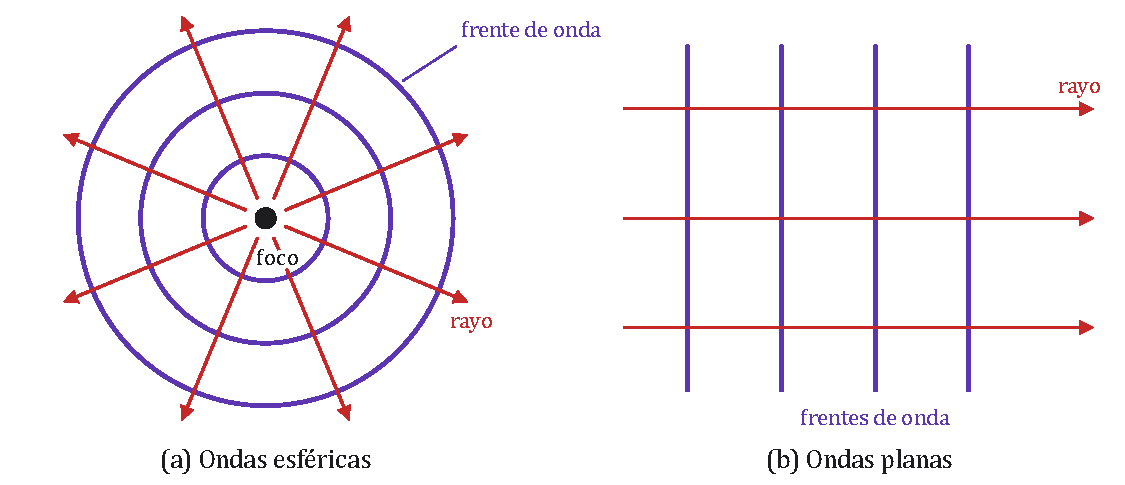
\includegraphics[width=0.85\linewidth]{images/UD2/frentes_rayos}
    \caption{Frentes de onda (en morado) y rayos (en rojo). Los rayos son siempre perpendiculares a los frentes.}
    \label{fig:ond-frentes}
\end{figure}

\section{Clasificación de las ondas}\label{sec:ond-clasificacion}

\begin{table}[H]
    \centering
    \caption{Clasificación de las ondas}
    \vspace{-5pt}
    \begin{tabular}{@{}L{3.6cm}L{3.2cm}L{6.6cm}@{}}
        \toprule
        \textbf{Criterio} & \textbf{Tipo} & \textbf{Características y ejemplos} \\
        \midrule
        \multirow{2}{3.6cm}{Duración de la perturbación} & Pulso & Perturbación breve: un golpe seco en el extremo de una cuerda. \\[3pt]
         & Tren de ondas & El foco vibra de forma continua: agitar sin parar el extremo de la cuerda. \\[3pt]
        \multirow{2}{3.6cm}{Dirección de vibración} & Longitudinales & Las partículas vibran en la dirección de propagación: muelle, sonido. \\[3pt]
         & Transversales & Vibran perpendicularmente a la propagación: cuerda, luz. \\[3pt]
        \multirow{2}{3.6cm}{Necesidad de medio} & Mecánicas & Necesitan un medio material: sonido, olas, ondas sísmicas. \\[3pt]
         & Electromagnéticas & Se propagan también en el vacío: luz, radio, rayos X. \\[3pt]
        \multirow{3}{3.6cm}{Dimensiones en que se propaga la energía} & Unidimensionales & A lo largo de una línea: cuerda, muelle. \\[3pt]
         & Bidimensionales & En una superficie: ondas en el agua. \\[3pt]
         & Tridimensionales & En todo el espacio: sonido, luz. \\
        \bottomrule
    \end{tabular}
    \label{tab:ond-clasificacion}
\end{table}

Las ondas longitudinales avanzan mediante \azuln{compresiones} (zonas donde las partículas se juntan) y
\azuln{dilataciones} (zonas donde se separan); por eso también se llaman \emph{ondas de presión}. En las transversales se
forman \azuln{crestas} y \azuln{valles} (figura~\ref{fig:ond-tipos}).

\begin{figure}[H]
    \centering
    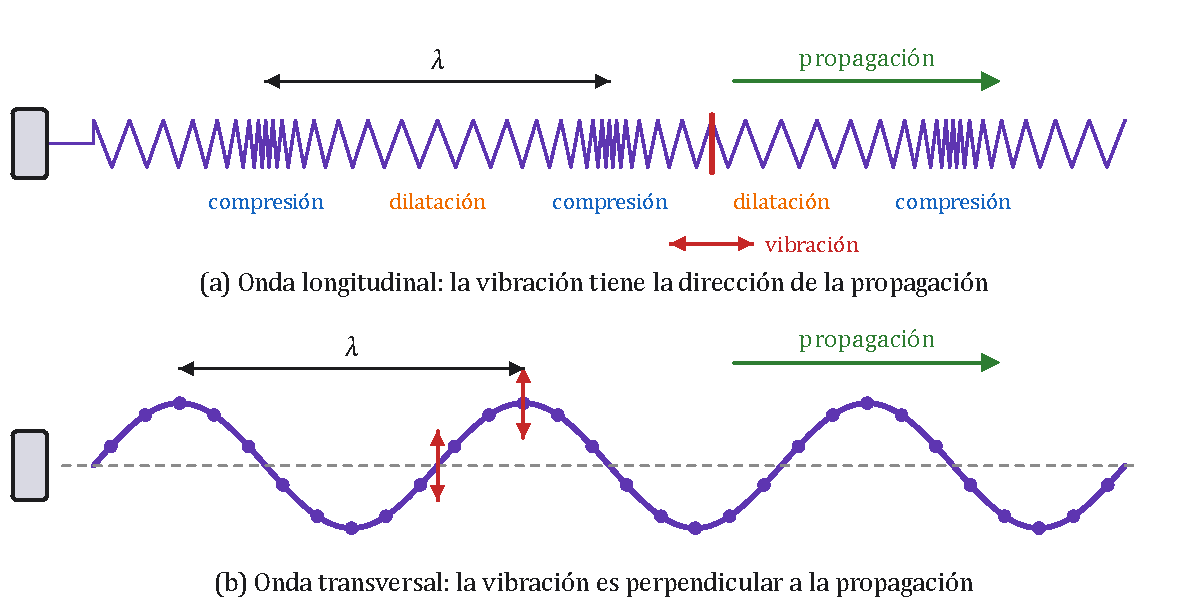
\includegraphics[width=0.95\linewidth]{images/UD2/tipos_onda}
    \caption{(a) En un muelle la vibración de cada espira tiene la misma dirección que la propagación. (b) En una cuerda cada
    punto sube y baja mientras la onda avanza en horizontal. En ambos casos \(\lambda\) es la distancia entre dos puntos que
    vibran igual.}
    \label{fig:ond-tipos}
\end{figure}

\section{Velocidad de propagación}\label{sec:ond-velocidad}

La velocidad con que avanza una onda depende \textbf{solo de las propiedades del medio} (su elasticidad y su inercia), no
de cómo vibre el foco. Si el medio es homogéneo, la velocidad es constante. Algunas expresiones (no hay que deducirlas):

\begin{table}[H]
    \centering
    \caption{Velocidad de propagación de las ondas en algunos medios}
    \vspace{-5pt}
    \begin{tabular}{@{}L{4.6cm}cL{6.4cm}@{}}
        \toprule
        \textbf{Onda} & \textbf{Velocidad} & \textbf{Magnitudes} \\
        \midrule
        Transversal en una cuerda & \(v = \sqrt{\dfrac{T}{\mu}}\) & \(T\): tensión (\unit{\newton}); \(\mu\): masa por unidad de longitud (\unit{\kg\per\m}) \\[10pt]
        Longitudinal en un muelle & \(v = l\sqrt{\dfrac{k}{m}}\) & \(k\): constante elástica; \(l\) y \(m\): longitud y masa del muelle \\[10pt]
        Longitudinal en un sólido & \(v = \sqrt{\dfrac{Y}{\rho}}\) & \(Y\): módulo de Young (\unit{\pascal}); \(\rho\): densidad \\[10pt]
        Sonido en un gas & \(v = \sqrt{\dfrac{\gamma R T}{M}}\) & \(\gamma\): coeficiente adiabático; \(T\): temperatura (\unit{\kelvin}); \(M\): masa molar (\unit{\kg\per\mol}) \\[10pt]
        Electromagnética & \(v = \dfrac{1}{\sqrt{\varepsilon\mu}}\) & \(\varepsilon\): permitividad; \(\mu\): permeabilidad magnética del medio \\
        \bottomrule
    \end{tabular}
    \label{tab:ond-velocidades}
\end{table}

Un medio en el que la onda se propagara sin perder energía sería \emph{perfectamente elástico}. Ningún medio real lo es:
el rozamiento entre partículas disipa energía y la onda se va \emph{amortiguando} (apartado~\ref{subsec:ond-amortiguacion}).

\begin{exercise}
    Una cuerda de guitarra tiene una masa de \qty{3.2}{\g} por cada metro y está tensada con una fuerza de \qty{72}{\newton}.
    Calcula la velocidad de las ondas transversales en ella. ¿Y la del sonido en el aire a \qty{20}{\celsius}?
    (\(\gamma = 1{,}4\); \(M = \qty{0.029}{\kg\per\mol}\); \(R = \qty{8.31}{\joule\per\mol\per\kelvin}\)).
    \begin{solu}
        \textcolor{blue}{Cuerda: \(\mu = \qty{3.2e-3}{\kg\per\m}\).}
        \(v = \sqrt{\dfrac{T}{\mu}} = \sqrt{\dfrac{72}{3{,}2\cdot 10^{-3}}} = \sqrt{22500} = \textcolor{red}{\qty{150}{\m\per\second}}\).

        \textcolor{blue}{Aire: \(T = \qty{293}{\kelvin}\).}
        \(v = \sqrt{\dfrac{1{,}4\cdot 8{,}31\cdot 293}{0{,}029}} = \textcolor{red}{\qty{343}{\m\per\second}}\).
    \end{solu}
\end{exercise}

\section{Magnitudes características de una onda}\label{sec:ond-magnitudes}

Pensemos en una onda armónica: el foco vibra con un m.a.s. y cada punto del medio repite ese m.a.s. con algo de retraso.

\begin{table}[H]
    \centering
    \caption{Magnitudes de una onda armónica}
    \vspace{-5pt}
    \begin{tabular}{@{}lcL{8cm}c@{}}
        \toprule
        \textbf{Magnitud} & \textbf{Símbolo} & \textbf{Significado} & \makecell{\textbf{Unidad} \\ \textbf{(SI)}} \\
        \midrule
        Elongación & \(y\) & Separación de un punto del medio respecto de su posición de equilibrio en un instante. & \unit{\m} \\[3pt]
        Amplitud & \(A\) & Elongación máxima; la misma que la del m.a.s. del foco (si no hay amortiguación). & \unit{\m} \\[3pt]
        Período & \(T\) & Tiempo que tarda cada punto en dar una vibración completa. & \unit{\second} \\[3pt]
        Frecuencia & \(\nu\) & Vibraciones por segundo de cada punto: \(\nu = 1/T\). & \unit{\hertz} \\[3pt]
        Pulsación & \(\omega\) & \(\omega = 2\pi/T = 2\pi\nu\). & \unit{\radian\per\second} \\[3pt]
        Longitud de onda & \(\lambda\) & Distancia que avanza la onda en un período. Es la distancia entre dos puntos consecutivos que vibran igual (dos crestas, dos compresiones). & \unit{\m} \\[3pt]
        Número de ondas & \(k\) & Número de longitudes de onda que caben en \(2\pi\) metros: \(k = 2\pi/\lambda\). & \unit{\per\m} \\[3pt]
        \makecell[l]{Velocidad de \\ propagación} & \(v\) & Distancia que avanza la onda por unidad de tiempo: \(v = \lambda/T = \lambda\nu\). & \unit{\m\per\second} \\
        \bottomrule
    \end{tabular}
    \label{tab:ond-magnitudes}
\end{table}

Como la onda avanza una longitud de onda en cada período:
\begin{centeredequation}
    \boxed{\lambda = v\,T = \dfrac{v}{\nu}} \qquad\qquad v = \dfrac{\omega}{k} \label{eq:ond-lambda}
\end{centeredequation}

\begin{figure}[H]
    \centering
    \begin{tikzpicture}
        \begin{axis}[fisica, width=0.8\linewidth, height=4.6cm, xmin=0, xmax=2.3, ymin=-1.5, ymax=1.6,
            xlabel={\(x\)}, ylabel={\(y\)}, xtick=\empty, ytick={-1,1}, yticklabels={\(-A\),\(A\)}]
            \addplot[domain=0:2.15, very thick, ocre] {sin(deg(2*pi*x))};
            \draw[<->, thick] (axis cs:0.25,1.3) -- node[above, font=\small]{\(\lambda\)} (axis cs:1.25,1.3);
            \draw[<->, thick] (axis cs:0.5,-1.3) -- node[below, font=\small]{\(\lambda\)} (axis cs:1.5,-1.3);
            \draw[<->, thick, blue] (axis cs:1.25,0) -- node[right, font=\small]{\(A\)} (axis cs:1.25,1);
            \draw[dashed, gray] (axis cs:0.25,1) -- (axis cs:0.25,1.3);
            \draw[dashed, gray] (axis cs:1.25,1) -- (axis cs:1.25,1.3);
            \node[font=\small, red] at (axis cs:1.75,-1.25) {valle};
            \node[font=\small, red] at (axis cs:2.05,1.25) {cresta};
        \end{axis}
    \end{tikzpicture}
    \caption{«Fotografía» de una onda transversal en un instante. La longitud de onda es la distancia entre dos crestas, dos
    valles o, en general, dos puntos consecutivos con el mismo estado de vibración.}
    \label{fig:ond-foto}
\end{figure}

\begin{remark}
    No hay que confundir dos velocidades distintas:
    \begin{itemize}
        \item la \textbf{velocidad de propagación} \(v = \lambda/T\), que es constante y depende del medio;
        \item la \textbf{velocidad de vibración} de cada partícula, \(v_y = dy/dt\), que cambia en cada instante (es la de un
        m.a.s.) y vale como máximo \(A\omega\).
    \end{itemize}
    El período, la frecuencia y la amplitud los fija el \textbf{foco}; la velocidad la fija el \textbf{medio}. La longitud
    de onda depende de los dos.
\end{remark}

\section{Ecuación de una onda armónica}\label{sec:ond-ecuacion}

La ecuación de una onda da la elongación \(y\) de cualquier punto del medio, situado a una distancia \(x\) del foco, en
cualquier instante \(t\): \(y = f(x, t)\).

Pongamos el foco en el origen, que la vibración sea en la dirección del eje \(Y\) y que la onda avance en el sentido positivo
del eje \(X\). Si el foco empieza a vibrar en su posición de equilibrio, su elongación es la de un m.a.s.:
\begin{equation*}
    y(0, t) = A\sen(\omega t)
\end{equation*}

Un punto situado a una distancia \(x\) empieza a vibrar con un retraso \(t' = x/v\), que es lo que tarda la onda en llegar
hasta él. Ese punto hace en el instante \(t\) lo mismo que hacía el foco en el instante \(t - t'\):
\begin{equation*}
    y(x, t) = y(0, t - t') = A\sen\left[\omega\left(t - \dfrac{x}{v}\right)\right]
\end{equation*}

Como \(\omega = 2\pi/T\), \(v\,T = \lambda\) y \(\omega/v = 2\pi/\lambda = k\), la misma ecuación se puede escribir de varias
formas equivalentes:
\begin{centeredequation}
    y(x,t) = A\sen\left[2\pi\left(\dfrac{t}{T} - \dfrac{x}{\lambda}\right)\right] = \boxed{A\sen(\omega t - k x)} \label{eq:ond-ecuacion}
\end{centeredequation}

\paragraph{Fase inicial.} Si en \(t = 0\) el foco no está en su posición de equilibrio, hay que añadir una fase inicial:
\begin{centeredequation}
    \boxed{y(x,t) = A\sen(\omega t - k x + \varphi_0)} \label{eq:ond-ecuacion-fase}
\end{centeredequation}
El ángulo \(\omega t - kx + \varphi_0\) es la \azuln{fase} de la onda: depende a la vez de la posición y del tiempo.

\paragraph{Sentido de propagación.} Si la onda avanza en el sentido \emph{negativo} del eje \(X\), el signo de \(kx\)
cambia:
\begin{equation*}
    y(x,t) = A\sen(\omega t + k x + \varphi_0)
\end{equation*}
Regla práctica: si \(\omega t\) y \(kx\) tienen \textbf{signos distintos}, la onda avanza hacia las \(x\) positivas; si
tienen el \textbf{mismo signo}, hacia las negativas.

\paragraph{Velocidad y aceleración de vibración.} Derivando respecto del tiempo (con \(x\) fijo):
\begin{equation*}
    v_y = \dfrac{\partial y}{\partial t} = A\omega\cos(\omega t - kx + \varphi_0) \qquad
    a_y = \dfrac{\partial v_y}{\partial t} = -A\omega^2\sen(\omega t - kx + \varphi_0) = -\omega^2 y
\end{equation*}
con valores máximos \(v_{y,\text{máx}} = A\omega\) y \(a_{y,\text{máx}} = A\omega^2\), como en un m.a.s.

\begin{exercise}
    Una onda que viaja por una cuerda tiene por ecuación, en unidades del SI, \(y = 0{,}03\sen(50t - 5x)\). Calcula la
    amplitud, la pulsación, la frecuencia, el período, la longitud de onda, la velocidad de propagación y la velocidad de
    vibración de un punto situado en \(x = \qty{20}{\cm}\) en el instante \(t = \qty{0.4}{\second}\).
    \begin{solu}
        \textcolor{blue}{Comparando con \(y = A\sen(\omega t - kx)\): \(A = \qty{0.03}{\m}\), \(\omega = \qty{50}{\radian\per\second}\), \(k = \qty{5}{\per\m}\).}

        \(\nu = \dfrac{\omega}{2\pi} = \textcolor{red}{\qty{7.96}{\hertz}}\); \(T = \dfrac{1}{\nu} = \textcolor{red}{\qty{0.126}{\second}}\);
        \(\lambda = \dfrac{2\pi}{k} = \textcolor{red}{\qty{1.26}{\m}}\); \(v = \dfrac{\omega}{k} = \textcolor{red}{\qty{10}{\m\per\second}}\).

        \textcolor{blue}{Velocidad de vibración: \(v_y = A\omega\cos(50t - 5x) = 1{,}5\cos(50t - 5x)\). En \(x = \qty{0.2}{\m}\), \(t = \qty{0.4}{\second}\) (calculadora en RAD):}
        \[ v_y = 1{,}5\cos(20 - 1) = 1{,}5\cos 19 = \textcolor{red}{\qty{1.48}{\m\per\second}} \]
    \end{solu}
\end{exercise}

\begin{exercise}
    La ecuación de una onda es \(y = 5\sen\left[10\pi\left(t - \dfrac{x}{40}\right)\right]\), con las longitudes en
    centímetros y el tiempo en segundos. Halla la amplitud, la frecuencia y la velocidad de propagación.
    \begin{solu}
        \textcolor{blue}{Comparando con \(y = A\sen\left[\omega\left(t - \dfrac{x}{v}\right)\right]\):}
        \(A = \textcolor{red}{\qty{5}{\cm}}\); \(\omega = 10\pi \Rightarrow \nu = \dfrac{10\pi}{2\pi} = \textcolor{red}{\qty{5}{\hertz}}\);
        \(v = \textcolor{red}{\qty{40}{\cm\per\second}}\).
    \end{solu}
\end{exercise}

\section{Doble periodicidad. Puntos en fase y en oposición}\label{sec:ond-periodicidad}

La ecuación de una onda es periódica respecto de dos variables:
\begin{itemize}
    \item \textbf{En el tiempo.} Si fijamos un punto (\(x\) constante) y cambiamos \(t\) por \(t + nT\), la fase aumenta en
    \(2\pi n\) y el seno no cambia: \emph{cada punto repite su estado de vibración cada período}.
    \item \textbf{En el espacio.} Si fijamos un instante (\(t\) constante) y cambiamos \(x\) por \(x + n\lambda\), la fase
    disminuye en \(2\pi n\): \emph{en cada instante, la forma de la onda se repite cada longitud de onda}.
\end{itemize}

\begin{figure}[H]
    \centering
    \begin{tikzpicture}
        \begin{axis}[fisica, width=0.47\linewidth, height=4.2cm, xmin=0, xmax=1.25, ymin=-1.35, ymax=1.5,
            xlabel={\(t\)}, ylabel={\(y\)}, xtick={0.5,1}, xticklabels={\(\frac{T}{2}\),\(T\)}, ytick={-1,1}, yticklabels={\(-A\),\(A\)},
            title={\small Un punto fijo (\(x\) constante)}]
            \addplot[domain=0:1.15, very thick, ocre] {sin(deg(2*pi*x))};
        \end{axis}
    \end{tikzpicture}\hfill
    \begin{tikzpicture}
        \begin{axis}[fisica, width=0.47\linewidth, height=4.2cm, xmin=0, xmax=1.25, ymin=-1.35, ymax=1.5,
            xlabel={\(x\)}, ylabel={\(y\)}, xtick={0.5,1}, xticklabels={\(\frac{\lambda}{2}\),\(\lambda\)}, ytick={-1,1}, yticklabels={\(-A\),\(A\)},
            title={\small Un instante fijo (\(t\) constante)}]
            \addplot[domain=0:1.15, very thick, blue] {-sin(deg(2*pi*x))};
        \end{axis}
    \end{tikzpicture}
    \caption{Doble periodicidad de una onda \(y = A\sen(\omega t - kx)\): la vibración de un punto se repite cada \(T\) y la
    forma de la onda se repite cada \(\lambda\).}
    \label{fig:ond-periodicidad}
\end{figure}

\paragraph{Concordancia y oposición de fase.} En un mismo instante, dos puntos situados en \(x_1\) y \(x_2\) tienen una
diferencia de fase:
\begin{equation*}
    \Delta\varphi = (\omega t - k x_1) - (\omega t - k x_2) = k\,(x_2 - x_1) = \dfrac{2\pi}{\lambda}\,\Delta x
\end{equation*}
\begin{itemize}
    \item Están \rojon{en fase} (misma elongación y misma velocidad) si \(\Delta\varphi = 2n\pi\), es decir, si
    \(\boxed{\Delta x = n\lambda}\): los separa un número entero de longitudes de onda.
    \item Están \rojon{en oposición de fase} (elongaciones y velocidades opuestas) si \(\Delta\varphi = (2n - 1)\pi\), es
    decir, si \(\boxed{\Delta x = (2n - 1)\,\dfrac{\lambda}{2}}\): los separa un número impar de semilongitudes de onda.
\end{itemize}
Del mismo modo, un mismo punto en dos instantes separados \(\Delta t\) tiene una diferencia de fase \(\Delta\varphi =
\omega\,\Delta t\).

\begin{exercise}
    Un foco vibra con una frecuencia de \qty{400}{\hertz} y produce ondas que se propagan a \qty{340}{\m\per\second}. Calcula:
    \begin{enumerate}[label=\letraminuscula]
        \item La distancia entre dos puntos próximos cuya diferencia de fase es \ang{60}.
        \item El tiempo que separa dos estados de vibración de un mismo punto con una diferencia de fase de \ang{180}.
        \item La diferencia de fase, en un instante dado, entre dos puntos separados \qty{2.55}{\m}.
    \end{enumerate}
    \begin{solu}
        \textcolor{blue}{\(\lambda = \dfrac{v}{\nu} = \dfrac{340}{400} = \qty{0.85}{\m}\); \(\omega = 2\pi\nu = 800\pi\ \unit{\radian\per\second}\).}
        \begin{enumerate}[label=\letraminuscula]
            \item \(\ang{60} = \dfrac{\pi}{3}\ \unit{\radian}\):
            \(\Delta x = \dfrac{\Delta\varphi}{2\pi}\,\lambda = \dfrac{\lambda}{6} = \textcolor{red}{\qty{0.142}{\m}}\).
            \item \(\Delta t = \dfrac{\Delta\varphi}{\omega} = \dfrac{\pi}{800\pi} = \textcolor{red}{\qty{1.25e-3}{\second}}\) (medio período).
            \item \(\Delta\varphi = \dfrac{2\pi}{\lambda}\,\Delta x = \dfrac{2\pi\cdot 2{,}55}{0{,}85} = \textcolor{red}{6\pi\ \unit{\radian}}\):
            \textcolor{blue}{los separan tres longitudes de onda, así que están en fase.}
        \end{enumerate}
    \end{solu}
\end{exercise}

\section{Energía e intensidad de una onda}\label{sec:ond-energia}

Cada partícula del medio vibra con un m.a.s., así que su energía es la de un oscilador
(ecuación~\eqref{eq:mas-energia}):
\begin{centeredequation}
    E = \dfrac{1}{2} k A^2 = \dfrac{1}{2} m\omega^2 A^2 = 2\pi^2 m\,\nu^2 A^2 \label{eq:ond-energia}
\end{centeredequation}
\begin{remark}
    La energía que transmite una onda es proporcional al \textbf{cuadrado de la amplitud} y al \textbf{cuadrado de la
    frecuencia}.
\end{remark}

\begin{definition}[Intensidad de una onda]
    La \rojon{intensidad} \(I\) es la energía que atraviesa, en cada unidad de tiempo, la unidad de superficie colocada
    perpendicularmente a la dirección de propagación. Es la potencia por unidad de superficie:
    \begin{centeredequation}
        \boxed{I = \dfrac{E}{S\,t} = \dfrac{P}{S}} \qquad \left[\unit{\watt\per\square\m}\right] \label{eq:ond-intensidad}
    \end{centeredequation}
\end{definition}

\paragraph{Atenuación con la distancia.} Si un foco puntual emite con potencia \(P\) en todas las direcciones y el medio no
absorbe energía, esa potencia se reparte en esferas cada vez mayores (figura~\ref{fig:ond-esferas}). A una distancia \(r\):
\begin{centeredequation}
    I = \dfrac{P}{4\pi r^2} \label{eq:ond-intensidad-r}
\end{centeredequation}

\begin{figure}[H]
    \centering
    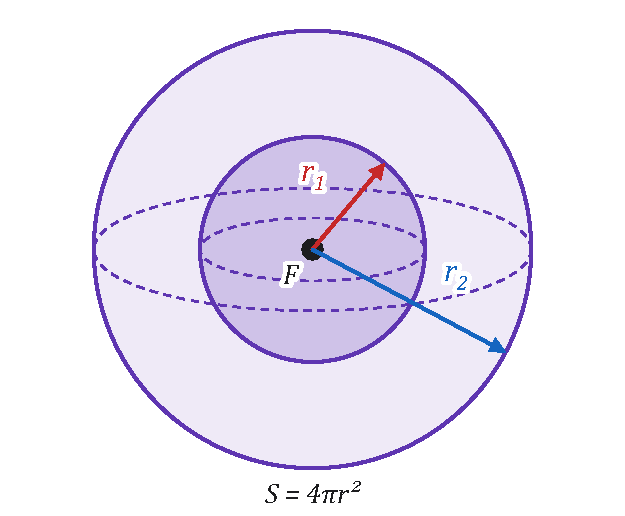
\includegraphics[width=0.38\linewidth]{images/UD2/intensidad_esferas}
    \caption{La misma potencia atraviesa las dos esferas. Como la mayor tiene más superficie, la intensidad en ella es menor.}
    \label{fig:ond-esferas}
\end{figure}

Igualando la potencia que atraviesa dos esferas de radios \(r_1\) y \(r_2\), \(I_1\,4\pi r_1^2 = I_2\,4\pi r_2^2\); y como
\(I\) es proporcional a \(A^2\):
\begin{centeredequation}
    \boxed{\dfrac{I_1}{I_2} = \dfrac{r_2^2}{r_1^2} = \dfrac{A_1^2}{A_2^2}} \qquad\Rightarrow\qquad \dfrac{A_1}{A_2} = \dfrac{r_2}{r_1} \label{eq:ond-atenuacion}
\end{centeredequation}
La intensidad disminuye con el cuadrado de la distancia y la amplitud, con la distancia.

\begin{exercise}
    Calcula la intensidad de una onda a \qty{4}{\m} de un foco puntual que emite con una potencia de \qty{60}{\watt}.
    \begin{solu}
        \(I = \dfrac{P}{4\pi r^2} = \dfrac{60}{4\pi\cdot 4^2} = \textcolor{red}{\qty{0.298}{\watt\per\square\m}}\).
    \end{solu}
\end{exercise}

\begin{exercise}
    A \qty{8}{\m} de un altavoz la intensidad del sonido es \qty{0.05}{\watt\per\square\m}. ¿Qué potencia tiene el altavoz?
    \begin{solu}
        \(P = I\cdot 4\pi r^2 = 0{,}05\cdot 4\pi\cdot 64 = \textcolor{red}{\qty{40.2}{\watt}}\).
    \end{solu}
\end{exercise}

\begin{exercise}
    Un foco emite ondas esféricas con una potencia de \qty{30}{\watt}. A \qty{3}{\m} del foco la amplitud es de \qty{2}{\cm}.
    ¿Cuánto valen la intensidad y la amplitud a \qty{6}{\m}?
    \begin{solu}
        \(I_6 = \dfrac{30}{4\pi\cdot 6^2} = \textcolor{red}{\qty{0.0663}{\watt\per\square\m}}\).
        \textcolor{blue}{Amplitud: \(\dfrac{A_6}{A_3} = \dfrac{r_3}{r_6} = \dfrac{3}{6}\)} \(\Rightarrow A_6 = \textcolor{red}{\qty{1}{\cm}}\).
        \textcolor{blue}{(Al doblar la distancia, la intensidad se divide entre 4 y la amplitud entre 2.)}
    \end{solu}
\end{exercise}

\subsection{Amortiguación}\label{subsec:ond-amortiguacion}

La amplitud de una onda disminuye al avanzar por dos causas:
\begin{itemize}
    \item \textbf{Atenuación}: en las ondas esféricas la energía se reparte entre cada vez más partículas, como acabamos de
    ver. Ocurre aunque el medio no absorba nada.
    \item \textbf{Absorción}: parte de la energía se pierde por rozamiento con las partículas del medio y se convierte en
    energía interna. La intensidad decrece exponencialmente con la distancia \(x\) recorrida en el medio:
    \begin{centeredequation}
        \boxed{I = I_0\,e^{-\beta x}} \label{eq:ond-absorcion}
    \end{centeredequation}
    donde \(I_0\) es la intensidad inicial y \(\beta\) el \azuln{coeficiente de absorción} del material (\unit{\per\m}).
\end{itemize}

\begin{exercise}
    Una onda pierde el \qty{25}{\percent} de su intensidad por absorción al atravesar \qty{8}{\cm} de un material. ¿Qué
    espesor de ese material reduce su intensidad a la mitad?
    \begin{solu}
        \textcolor{blue}{Si pierde el \qty{25}{\percent}, queda \(I = 0{,}75\,I_0\):}
        \(0{,}75 = e^{-\beta\cdot 0{,}08} \Rightarrow \beta = \dfrac{-\ln 0{,}75}{0{,}08} = \qty{3.60}{\per\m}\).

        \textcolor{blue}{Para \(I = I_0/2\):} \(x = \dfrac{\ln 2}{\beta} = \dfrac{0{,}693}{3{,}60} = \textcolor{red}{\qty{0.193}{\m} \approx \qty{19}{\cm}}\).
    \end{solu}
\end{exercise}

\section{El sonido}\label{sec:ond-sonido}

El \rojon{sonido} es una onda \textbf{mecánica}, \textbf{longitudinal} y \textbf{tridimensional}: un cuerpo vibra y produce
compresiones y dilataciones del medio que lo rodea (aire, agua, un sólido\ldots) que se propagan en todas direcciones. En el
vacío no hay sonido. Su velocidad en el aire es de unos \qty{340}{\m\per\second}; en el agua, unos \qty{1450}{\m\per\second}, y
en el acero, unos \qty{5000}{\m\per\second}.

El oído humano percibe vibraciones con frecuencias entre \qty{20}{\hertz} y \qty{20000}{\hertz}. Según la frecuencia:
\begin{itemize}
    \item \textbf{Infrasonidos}: \(\nu < \qty{20}{\hertz}\) (terremotos, algunos animales como los elefantes).
    \item \textbf{Sonidos audibles}: entre \qty{20}{\hertz} y \qty{20000}{\hertz}.
    \item \textbf{Ultrasonidos}: \(\nu > \qty{20000}{\hertz}\) (ecografías, sónar, murciélagos y delfines).
\end{itemize}

\paragraph{Eco.} El oído distingue dos sonidos como distintos si le llegan separados al menos una décima de segundo. Si un
sonido corto se refleja en un obstáculo y vuelve pasado ese tiempo, se oye repetido: es el \azuln{eco}. Con
\(v = \qty{340}{\m\per\second}\), el sonido recorre \qty{34}{\m} en \qty{0.1}{\second} (ida y vuelta), así que el obstáculo
debe estar al menos a \qty{17}{\m}. Si está más cerca, el sonido reflejado se superpone al original y lo alarga: es la
\azuln{reverberación}.

\begin{exercise}
    Al gritar frente a un acantilado oyes el eco \qty{3}{\second} después. ¿A qué distancia está? (\(v = \qty{340}{\m\per\second}\)).
    \begin{solu}
        \textcolor{blue}{El sonido va y vuelve: recorre \(2d\) en \qty{3}{\second}.}
        \(2d = 340\cdot 3 \Rightarrow d = \textcolor{red}{\qty{510}{\m}}\).
    \end{solu}
\end{exercise}

\begin{exercise}
    ¿Entre qué longitudes de onda están los sonidos que puede oír una persona? (\(v = \qty{340}{\m\per\second}\)).
    \begin{solu}
        \(\lambda = \dfrac{v}{\nu}\): \(\lambda_{\text{máx}} = \dfrac{340}{20} = \textcolor{red}{\qty{17}{\m}}\);
        \(\lambda_{\text{mín}} = \dfrac{340}{20000} = \textcolor{red}{\qty{1.7}{\cm}}\).
    \end{solu}
\end{exercise}

\begin{exercise}
    Un coche se dirige hacia una montaña a \qty{90}{\km\per\hour}, toca el claxon y recibe el eco \qty{3}{\second} después.
    ¿A qué distancia de la montaña está cuando oye el eco?
    \begin{solu}
        \textcolor{blue}{\(v_c = \qty{25}{\m\per\second}\). Sea \(d_0\) la distancia al tocar el claxon. En \qty{3}{\second} el
        sonido recorre \(340\cdot 3 = \qty{1020}{\m}\) y el coche \(25\cdot 3 = \qty{75}{\m}\). El sonido va hasta la montaña
        (\(d_0\)) y vuelve hasta el coche (\(d_0 - 75\)):}
        \[ 2d_0 - 75 = 1020 \;\Rightarrow\; d_0 = \qty{547.5}{\m} \]
        \textcolor{blue}{Al oír el eco está a} \(547{,}5 - 75 = \textcolor{red}{\qty{472.5}{\m}}\).
    \end{solu}
\end{exercise}

\begin{exercise}
    Una locomotora avanza hacia un túnel con velocidad constante. El maquinista hace sonar el silbato y oye el eco del
    túnel \qty{6}{\second} después. En ese momento vuelve a silbar y el segundo eco le llega \qty{5}{\second} más tarde.
    ¿Qué velocidad lleva? (\(v = \qty{340}{\m\per\second}\)).
    \begin{solu}
        \textcolor{blue}{Sea \(u\) la velocidad del tren y \(D\) la distancia en el primer silbido. Como en la actividad
        anterior, \(2D - 6u = 6\cdot 340\), luego \(D = 3(340 + u)\). Al segundo silbido la distancia es
        \(D' = D - 6u = 3(340 - u)\), y con el segundo eco:}
        \[ 2D' - 5u = 5\cdot 340 \;\Rightarrow\; 6\cdot 340 - 6u - 5u = 5\cdot 340 \;\Rightarrow\; 11u = 340 \]
        \(u = \textcolor{red}{\qty{30.9}{\m\per\second} \approx \qty{111}{\km\per\hour}}\).
    \end{solu}
\end{exercise}

\subsection{Cualidades del sonido}\label{subsec:ond-cualidades}

\begin{itemize}
    \item \textbf{Tono} (o altura): distingue los sonidos \emph{agudos} (frecuencia alta) de los \emph{graves} (frecuencia
    baja). Depende de la frecuencia.
    \item \textbf{Timbre}: permite distinguir la misma nota tocada por un violín y por una flauta. Un instrumento no emite
    una sola frecuencia sino la fundamental acompañada de sus armónicos (apartado~\ref{subsec:ond-armonicos}), en
    proporciones distintas; el timbre depende de la \emph{forma} de la onda.
    \item \textbf{Intensidad} (o sonoridad): distingue los sonidos fuertes de los débiles. Depende de la amplitud.
\end{itemize}

\subsection{Nivel de intensidad sonora}\label{subsec:ond-decibelios}

El oído percibe sonidos muy débiles, desde \(I_0 = \qty{e-12}{\watt\per\square\m}\) (\azuln{umbral de audición}), hasta
unos \qty{1}{\watt\per\square\m} (\azuln{umbral de dolor}): un intervalo de doce órdenes de magnitud. Además, la sensación
sonora no crece en proporción a la intensidad: un sonido de doble intensidad no se oye «el doble de fuerte». Por eso se usa
una escala logarítmica.

\begin{definition}[Nivel de intensidad sonora]
    El \rojon{nivel de intensidad sonora} (o sonoridad) \(\beta\) de un sonido de intensidad \(I\) es:
    \begin{centeredequation}
        \boxed{\beta = 10\log\dfrac{I}{I_0}} \qquad I_0 = \qty{e-12}{\watt\per\square\m} \label{eq:ond-decibelios}
    \end{centeredequation}
    Se mide en \azuln{decibelios} (\unit{\deci\bel}). El umbral de audición corresponde a \qty{0}{\deci\bel} y el de dolor a
    \qty{120}{\deci\bel}.
\end{definition}

\begin{remark}
    Cada vez que la intensidad se multiplica por 10, el nivel sube \qty{10}{\deci\bel}; si se duplica, sube \qty{3}{\deci\bel}.
    Para despejar la intensidad: \(I = I_0\cdot 10^{\beta/10}\).
\end{remark}

\begin{exercise}
    ¿Qué nivel de intensidad sonora tiene un sonido de \qty{0.5}{\watt\per\square\m}?
    \begin{solu}
        \(\beta = 10\log\dfrac{0{,}5}{10^{-12}} = 10\log(5\cdot 10^{11}) = \textcolor{red}{\qty{117}{\deci\bel}}\),
        \textcolor{blue}{muy cerca del umbral de dolor.}
    \end{solu}
\end{exercise}

\begin{exercise}
    En una discoteca se miden \qty{105}{\deci\bel}. ¿Cuál es la intensidad sonora media?
    \begin{solu}
        \(I = I_0\cdot 10^{\beta/10} = 10^{-12}\cdot 10^{10{,}5} = \textcolor{red}{\qty{0.0316}{\watt\per\square\m}}\).
    \end{solu}
\end{exercise}

\begin{exercise}
    Demuestra que un sonido de \qty{80}{\deci\bel} es mil veces más intenso que uno de \qty{50}{\deci\bel}.
    \begin{solu}
        \textcolor{blue}{Restando los niveles:}
        \[ \beta_1 - \beta_2 = 10\log\dfrac{I_1}{I_0} - 10\log\dfrac{I_2}{I_0} = 10\log\dfrac{I_1}{I_2} = 80 - 50 = 30 \]
        \(\log\dfrac{I_1}{I_2} = 3 \Rightarrow \textcolor{red}{I_1 = 1000\,I_2}\).
    \end{solu}
\end{exercise}

\paragraph{Contaminación acústica.} Llamamos \emph{ruido} a los sonidos desagradables, formados por frecuencias sin relación
entre sí. Se mide con un \emph{sonómetro}, que da el nivel en decibelios. Estar mucho tiempo expuesto a niveles altos,
aunque no lleguen al umbral de dolor, produce pérdida progresiva de audición, estrés, falta de concentración, irritabilidad o
insomnio. La Organización Mundial de la Salud recomienda no superar unos \qty{55}{\deci\bel} de día y \qty{35}{\deci\bel} de
noche en las viviendas, y se habla de contaminación acústica cuando el nivel ambiental supera los \qty{70}{\deci\bel} durante
mucho tiempo.

\begin{table}[H]
    \centering
    \caption{Niveles de intensidad sonora aproximados}
    \vspace{-5pt}
    \begin{tabular}{@{}lcc@{}}
        \toprule
        \textbf{Fuente sonora} & \textbf{Nivel (\unit{\deci\bel})} & \textbf{Intensidad (\unit{\watt\per\square\m})} \\
        \midrule
        Umbral de audición & 0 & \num{e-12} \\[3pt]
        Biblioteca, casa tranquila & 40 & \num{e-8} \\[3pt]
        Conversación normal & 60 & \num{e-6} \\[3pt]
        Calle con mucho tráfico & 80 & \num{e-4} \\[3pt]
        Concierto, discoteca & 110 & \num{e-1} \\[3pt]
        Umbral de dolor & 120 & 1 \\[3pt]
        Despegue de un avión a reacción (cerca) & 140 & \num{e2} \\
        \bottomrule
    \end{tabular}
    \label{tab:ond-niveles}
\end{table}

\section{Interferencias}\label{sec:ond-interferencias}

Cuando dos o más ondas coinciden en un punto del medio se produce una \rojon{interferencia}. Lo característico es que, tras
cruzarse, cada onda sigue su camino como si la otra no hubiera existido.

\begin{definition}[Principio de superposición]
    Cuando varias ondas coinciden en un punto, la elongación resultante es la suma de las elongaciones que produciría cada
    onda por separado: \(y = y_1 + y_2 + \cdots\)
\end{definition}

Si las dos perturbaciones llegan en fase se refuerzan: la interferencia es \rojon{constructiva}. Si llegan en oposición de
fase se debilitan (o se anulan, si tienen la misma amplitud): la interferencia es \rojon{destructiva}
(figura~\ref{fig:ond-pulsos}).

\begin{figure}[H]
    \centering
    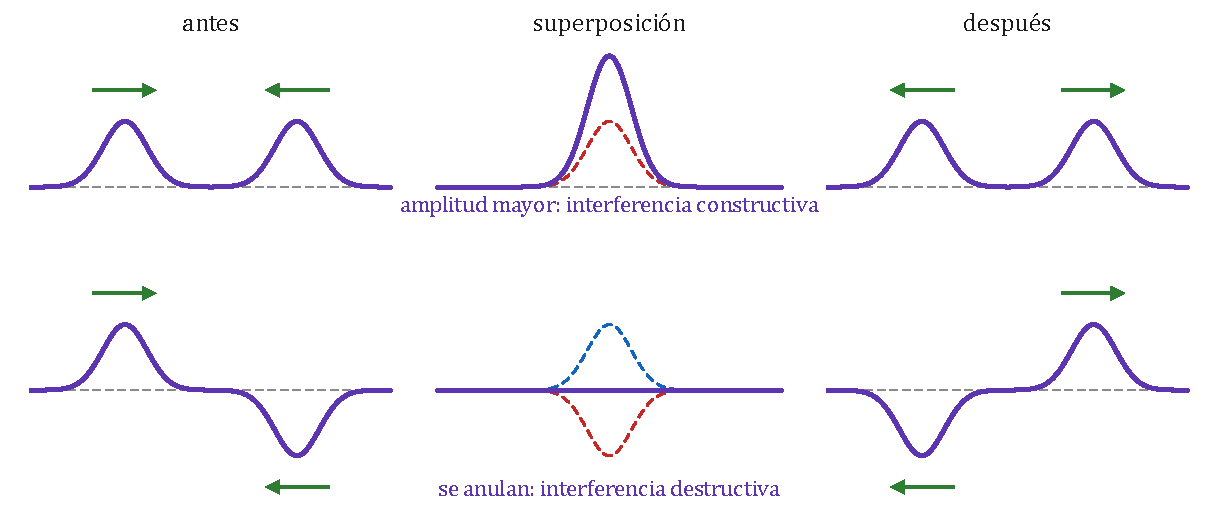
\includegraphics[width=0.9\linewidth]{images/UD2/interferencia_pulsos}
    \caption{Dos pulsos que se cruzan. Mientras coinciden, la forma de la cuerda es la suma de los dos (en discontinuo, cada
    pulso por separado). Después, cada uno sigue igual que antes.}
    \label{fig:ond-pulsos}
\end{figure}

\paragraph{Dos ondas de distinta amplitud.} Si en un punto coinciden dos m.a.s. de la misma frecuencia, con amplitudes
\(A_1\) y \(A_2\) y diferencia de fase \(\delta\), el resultado es otro m.a.s. de la misma frecuencia cuya amplitud se obtiene
sumando vectorialmente los dos \azuln{fasores} (vectores de módulo igual a la amplitud que giran con la fase):
\begin{centeredequation}
    A^2 = A_1^2 + A_2^2 + 2A_1A_2\cos\delta \label{eq:ond-fasores}
\end{centeredequation}
Si \(\delta = 2n\pi\), \(A = A_1 + A_2\) (máxima); si \(\delta = (2n - 1)\pi\), \(A = |A_1 - A_2|\) (mínima).

\subsection{Interferencia de dos ondas coherentes}\label{subsec:ond-coherentes}

Dos focos son \azuln{coherentes} si emiten ondas de la misma frecuencia con una diferencia de fase constante. Estudiaremos
el caso más sencillo: dos focos \(F_1\) y \(F_2\) que vibran en fase con la misma amplitud \(A\). A un punto \(P\) situado a
distancias \(x_1\) y \(x_2\) de los focos (figura~\ref{fig:ond-focos}) llegan:
\begin{equation*}
    y_1 = A\sen(\omega t - k x_1) \qquad\qquad y_2 = A\sen(\omega t - k x_2)
\end{equation*}

\begin{figure}[H]
    \centering
    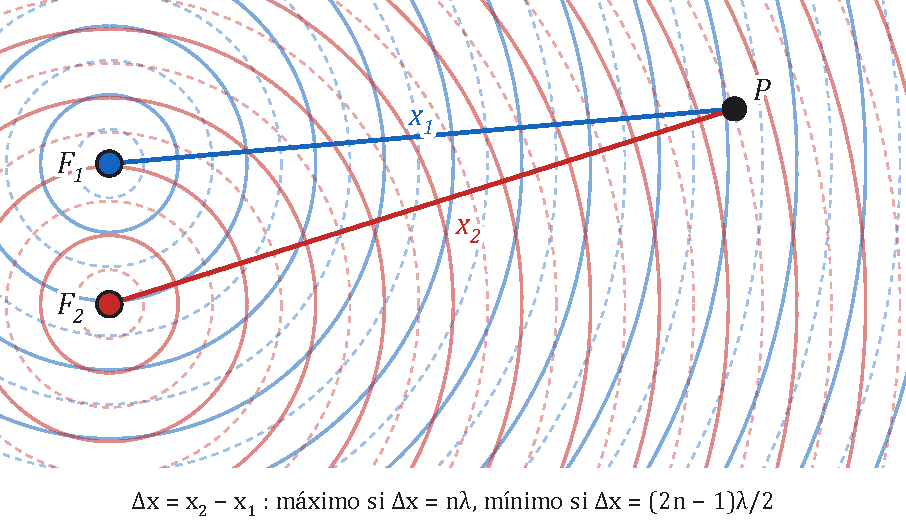
\includegraphics[width=0.6\linewidth]{images/UD2/interferencia_focos}
    \caption{Ondas emitidas por dos focos coherentes (crestas en línea continua y valles en discontinua). Lo que ocurre en
    \(P\) depende de la diferencia de caminos \(x_2 - x_1\).}
    \label{fig:ond-focos}
\end{figure}

Sumándolas con \(\sen a + \sen b = 2\sen\dfrac{a + b}{2}\cos\dfrac{a - b}{2}\):
\begin{centeredequation}
    y = \underbrace{2A\cos\left[\dfrac{k(x_2 - x_1)}{2}\right]}_{A_r}\,\sen\left[\omega t - k\,\dfrac{x_1 + x_2}{2}\right] \label{eq:ond-interferencia}
\end{centeredequation}
En \(P\) hay un m.a.s. de la misma frecuencia que las ondas, con una amplitud \(A_r\) que depende de la \textbf{diferencia de
caminos} \(\Delta x = x_2 - x_1\):
\begin{itemize}
    \item \textbf{Interferencia constructiva} (amplitud máxima, \(2A\)): \(\cos\dfrac{k\,\Delta x}{2} = \pm 1\), es decir,
    \[ \boxed{x_2 - x_1 = n\lambda} \qquad (n = 0, 1, 2\ldots) \]
    \item \textbf{Interferencia destructiva} (amplitud nula): \(\cos\dfrac{k\,\Delta x}{2} = 0\), es decir,
    \[ \boxed{x_2 - x_1 = (2n - 1)\,\dfrac{\lambda}{2}} \qquad (n = 1, 2, 3\ldots) \]
\end{itemize}

\begin{exercise}
    Dos altavoces conectados al mismo amplificador emiten en fase un sonido de \qty{680}{\hertz}
    (\(v = \qty{340}{\m\per\second}\)). ¿Qué tipo de interferencia hay en un punto que está a \qty{3}{\m} de un altavoz y a
    \qty{4.25}{\m} del otro? ¿Y en otro que está a \qty{3}{\m} y \qty{4}{\m}?
    \begin{solu}
        \textcolor{blue}{\(\lambda = \dfrac{v}{\nu} = \dfrac{340}{680} = \qty{0.5}{\m}\).}
        \begin{itemize}
            \item \(\Delta x = \qty{1.25}{\m} = 2{,}5\,\lambda = 5\cdot\dfrac{\lambda}{2}\): número impar de semilongitudes de onda,
            \textcolor{red}{interferencia destructiva} (apenas se oye).
            \item \(\Delta x = \qty{1}{\m} = 2\lambda\): \textcolor{red}{interferencia constructiva} (se oye más fuerte).
        \end{itemize}
    \end{solu}
\end{exercise}

\section{Ondas estacionarias}\label{sec:ond-estacionarias}

\begin{definition}[Onda estacionaria]
    Una \rojon{onda estacionaria} es el resultado de la interferencia de dos ondas iguales (misma amplitud, frecuencia y
    longitud de onda) que se propagan en la misma dirección y en sentidos contrarios.
\end{definition}

Es lo que ocurre en una cuerda sujeta por sus extremos, como la de una guitarra: las ondas se reflejan en los extremos y
las que van y las que vuelven se superponen.

\paragraph{Ecuación.} Tomemos el origen en el extremo fijo de una cuerda. La onda que llega viaja hacia las \(x\) negativas,
\(y_1 = A\sen(\omega t + kx)\). Al reflejarse en un extremo fijo cambia su fase en \(\pi\) (apartado~\ref{sec:ond-reflexion}),
así que la onda reflejada es \(y_2 = A\sen(\omega t - kx + \pi) = -A\sen(\omega t - kx)\). Sumando, con
\(\sen a - \sen b = 2\cos\dfrac{a + b}{2}\sen\dfrac{a - b}{2}\):
\begin{centeredequation}
    \boxed{y = 2A\sen(kx)\cos(\omega t)} \label{eq:ond-estacionaria}
\end{centeredequation}

Esta ecuación ya no tiene la forma \(\sen(\omega t \mp kx)\): no describe algo que avance. Cada punto vibra con un m.a.s. de
pulsación \(\omega\), pero con una amplitud que depende de su posición:
\begin{equation*}
    A_r = 2A\sen(kx)
\end{equation*}

\begin{itemize}
    \item \textbf{Nodos}: puntos que no vibran nunca (\(A_r = 0\)). \(\sen kx = 0 \Rightarrow kx = n\pi\):
    \[ \boxed{x = n\,\dfrac{\lambda}{2}} \qquad (n = 0, 1, 2\ldots) \]
    \item \textbf{Vientres} (o antinodos): puntos que vibran con la amplitud máxima, \(2A\). \(\sen kx = \pm 1 \Rightarrow
    kx = (2n - 1)\dfrac{\pi}{2}\):
    \[ \boxed{x = (2n - 1)\,\dfrac{\lambda}{4}} \qquad (n = 1, 2, 3\ldots) \]
\end{itemize}
Dos nodos (o dos vientres) consecutivos están separados \(\lambda/2\), y un nodo y el vientre siguiente, \(\lambda/4\)
(figura~\ref{fig:ond-estacionaria}).

\begin{figure}[H]
    \centering
    \begin{tikzpicture}
        \begin{axis}[fisica, width=0.8\linewidth, height=4.6cm, xmin=0, xmax=2.2, ymin=-1.5, ymax=1.6,
            xlabel={\(x\)}, ylabel={\(y\)}, xtick={0.5,1,1.5,2}, xticklabels={\(\frac{\lambda}{2}\),\(\lambda\),\(\frac{3\lambda}{2}\),\(2\lambda\)},
            ytick={-1,1}, yticklabels={\(-2A\),\(2A\)}]
            \pgfplotsinvokeforeach{0.5, -0.5, -1}{ \addplot[domain=0:2, thick, ocre!50, samples=120] {#1*sin(deg(2*pi*x))}; }
            \addplot[domain=0:2, very thick, ocre, samples=120] {sin(deg(2*pi*x))};
            \pgfplotsinvokeforeach{0, 0.5, 1, 1.5, 2}{ \node[circle, fill=blue, inner sep=1.6pt] at (axis cs:#1,0) {}; }
            \node[font=\small, blue, below] at (axis cs:0.5,-0.05) {N};
            \node[font=\small, red, above] at (axis cs:0.25,1.05) {V};
            \node[font=\small, red, above] at (axis cs:0.75,1.05) {V};
        \end{axis}
    \end{tikzpicture}
    \caption{Onda estacionaria en varios instantes. Los nodos (N) están siempre quietos; los vientres (V) oscilan con la
    amplitud máxima. Todos los puntos entre dos nodos vibran en fase.}
    \label{fig:ond-estacionaria}
\end{figure}

\begin{remark}
    Una onda estacionaria \textbf{no transporta energía} de un sitio a otro: la energía queda «atrapada» entre los nodos.
    No es, en sentido estricto, un movimiento ondulatorio, sino una forma de vibrar de todo el medio.
\end{remark}

Si las dos ondas que se superponen son \(y_1 = A\sen(\omega t + kx)\) e \(y_2 = A\sen(\omega t - kx)\) (sin el cambio de
fase), se obtiene \(y = 2A\cos(kx)\sen(\omega t)\). En ese caso los papeles se intercambian: hay un vientre en \(x = 0\), los
vientres están en \(x = n\lambda/2\) y los nodos en \(x = (2n - 1)\lambda/4\). Esta forma aparece, por ejemplo, en el
extremo abierto de un tubo.

\begin{exercise}
    Una cuerda vibra según la ecuación \(y = 4\sen\left(\dfrac{\pi}{4}x\right)\cos(30\pi t)\), con \(x\) e \(y\) en
    centímetros y \(t\) en segundos. Calcula:
    \begin{enumerate}[label=\letraminuscula]
        \item La amplitud y la velocidad de las ondas que la forman.
        \item La velocidad de vibración del punto \(x = \qty{1}{\cm}\) en \(t = \qty{0.05}{\second}\).
        \item La amplitud de un vientre y la distancia entre dos nodos consecutivos.
        \item La distancia entre el primer nodo (\(x = 0\)) y el tercer vientre.
    \end{enumerate}
    \begin{solu}
        \textcolor{blue}{Comparando con \(y = 2A\sen(kx)\cos(\omega t)\): \(2A = \qty{4}{\cm}\), \(k = \dfrac{\pi}{4}\ \unit{\per\cm}\), \(\omega = 30\pi\ \unit{\radian\per\second}\).}
        \begin{enumerate}[label=\letraminuscula]
            \item \(A = \textcolor{red}{\qty{2}{\cm}}\). \(\lambda = \dfrac{2\pi}{k} = \qty{8}{\cm}\), \(\nu = \dfrac{\omega}{2\pi} = \qty{15}{\hertz}\):
            \(v = \lambda\nu = \textcolor{red}{\qty{120}{\cm\per\second} = \qty{1.2}{\m\per\second}}\).
            \item \(v_y = \dfrac{\partial y}{\partial t} = -4\cdot 30\pi\sen\left(\dfrac{\pi}{4}x\right)\sen(30\pi t)\).
            Con \(x = 1\), \(t = 0{,}05\): \(v_y = -120\pi\cdot\sen\dfrac{\pi}{4}\cdot\sen\dfrac{3\pi}{2} = \textcolor{red}{\qty{267}{\cm\per\second}}\).
            \item Vientre: \(2A = \textcolor{red}{\qty{4}{\cm}}\). Entre nodos: \(\dfrac{\lambda}{2} = \textcolor{red}{\qty{4}{\cm}}\).
            \item \textcolor{blue}{Los vientres están en \(x = (2n - 1)\lambda/4 = 2, 6, 10\ldots\) cm.} El tercero está a \textcolor{red}{\qty{10}{\cm}} del primer nodo.
        \end{enumerate}
    \end{solu}
\end{exercise}

\begin{exercise}
    Para la onda estacionaria \(y = 2A\cos(kx)\sen(\omega t)\), deduce dónde están los vientres y los nodos y la distancia
    entre dos nodos consecutivos.
    \begin{solu}
        \textcolor{blue}{La amplitud es \(A_r = 2A\cos kx\).}
        \begin{itemize}
            \item Vientres: \(\cos kx = \pm 1 \Rightarrow kx = n\pi \Rightarrow \textcolor{red}{x = n\,\dfrac{\lambda}{2}}\) (\(n = 0, 1, 2\ldots\)).
            \item Nodos: \(\cos kx = 0 \Rightarrow kx = (2n - 1)\dfrac{\pi}{2} \Rightarrow \textcolor{red}{x = (2n - 1)\,\dfrac{\lambda}{4}}\).
            \item Entre nodos consecutivos: \(\dfrac{3\lambda}{4} - \dfrac{\lambda}{4} = \textcolor{red}{\dfrac{\lambda}{2}}\), igual que antes.
        \end{itemize}
    \end{solu}
\end{exercise}

\subsection{Armónicos}\label{subsec:ond-armonicos}

En una cuerda de longitud \(L\) no se puede formar cualquier onda estacionaria: los extremos imponen condiciones
(figura~\ref{fig:ond-armonicos}).

\paragraph{Cuerda con los dos extremos fijos} (guitarra, piano, violín). Los dos extremos tienen que ser nodos, así que en
la cuerda debe caber un número entero de semilongitudes de onda:
\begin{equation*}
    L = n\,\dfrac{\lambda}{2} \;\Rightarrow\; \lambda_n = \dfrac{2L}{n} \;\Rightarrow\; \boxed{\nu_n = \dfrac{v}{\lambda_n} = n\,\dfrac{v}{2L} = n\,\nu_1} \qquad (n = 1, 2, 3\ldots)
\end{equation*}
La frecuencia más baja, \(\nu_1 = v/2L\), es la \azuln{frecuencia fundamental} (o primer armónico). Las demás son múltiplos
enteros de ella: son los \azuln{armónicos}.

\paragraph{Cuerda con un extremo fijo y otro libre} (y también un tubo cerrado por un extremo). El extremo fijo es un nodo y
el libre es un vientre, así que la longitud debe ser un número impar de cuartos de longitud de onda:
\begin{equation*}
    L = (2n - 1)\,\dfrac{\lambda}{4} \;\Rightarrow\; \lambda = \dfrac{4L}{2n - 1} \;\Rightarrow\; \boxed{\nu = (2n - 1)\,\dfrac{v}{4L}} \qquad (n = 1, 2, 3\ldots)
\end{equation*}
Solo aparecen los armónicos \textbf{impares} de la fundamental \(\nu_1 = v/4L\): el tercero (\(n = 2\)), el quinto (\(n = 3\))\ldots

\begin{figure}[H]
    \centering
    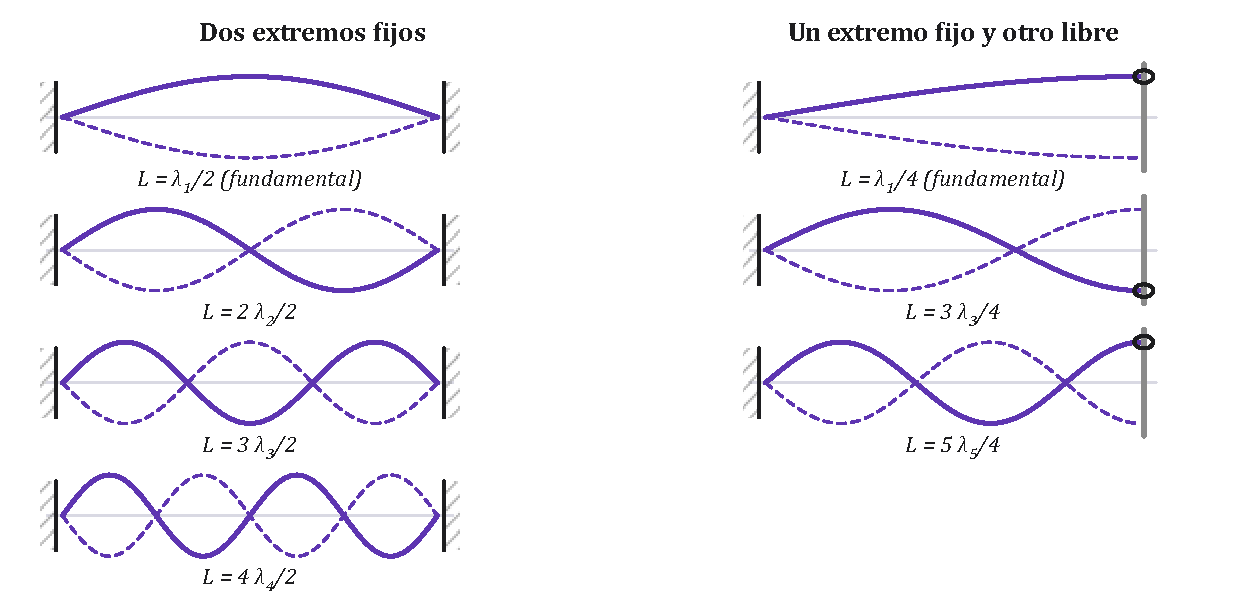
\includegraphics[width=0.95\linewidth]{images/UD2/armonicos}
    \caption{Modos de vibración de una cuerda de longitud \(L\). Con los dos extremos fijos caben \(n\) husos de longitud
    \(\lambda/2\); con un extremo libre, un número impar de cuartos de onda.}
    \label{fig:ond-armonicos}
\end{figure}

\begin{exercise}
    La cuerda La de una guitarra mide \qty{65}{\cm} entre sus dos apoyos y su frecuencia fundamental es \qty{110}{\hertz}.
    Calcula la velocidad de las ondas en la cuerda y las frecuencias de sus dos armónicos siguientes.
    \begin{solu}
        \textcolor{blue}{Fundamental: \(\lambda_1 = 2L = \qty{1.30}{\m}\).} \(v = \lambda_1\nu_1 = 1{,}30\cdot 110 = \textcolor{red}{\qty{143}{\m\per\second}}\).

        \(\nu_2 = 2\nu_1 = \textcolor{red}{\qty{220}{\hertz}}\); \(\nu_3 = 3\nu_1 = \textcolor{red}{\qty{330}{\hertz}}\).
        \textcolor{blue}{(Al pisar un traste se acorta \(L\) y sube la frecuencia.)}
    \end{solu}
\end{exercise}

\section{Principio de Huygens}\label{sec:ond-huygens}

En 1678 Christiaan Huygens propuso un método geométrico para saber cómo avanza un frente de onda. Cuando la onda alcanza un
punto, éste empieza a vibrar y se comporta como un nuevo foco que emite pequeñas ondas, las \azuln{ondas secundarias}.

\begin{definition}[Principio de Huygens]
    Cada punto de un frente de onda se comporta como un foco de ondas secundarias. Al cabo de un tiempo, el nuevo frente de
    onda es la superficie tangente a todas esas ondas secundarias (su \azuln{envolvente}).
\end{definition}

\begin{figure}[H]
    \centering
    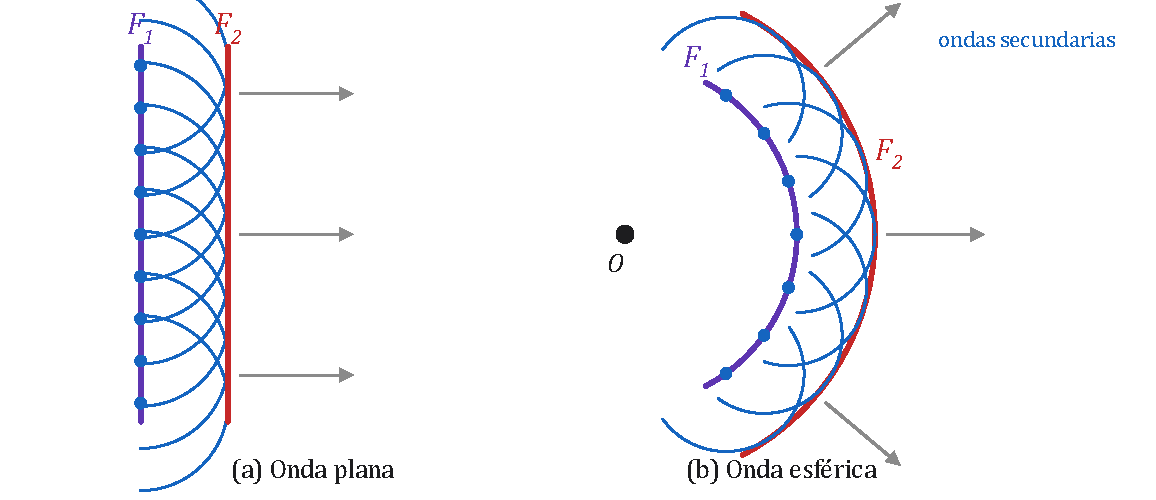
\includegraphics[width=0.85\linewidth]{images/UD2/huygens}
    \caption{Construcción de Huygens. Los puntos del frente \(F_1\) emiten ondas secundarias; su envolvente es el frente
    \(F_2\). Con este principio se explican la difracción, la reflexión y la refracción.}
    \label{fig:ond-huygens}
\end{figure}

\section{Difracción}\label{sec:ond-difraccion}

\begin{definition}[Difracción]
    La \rojon{difracción} es la desviación que sufre una onda al encontrar un obstáculo o una abertura: la onda lo rodea y
    se propaga también por detrás. Es apreciable cuando el tamaño del obstáculo o de la abertura es \textbf{parecido a la
    longitud de onda}.
\end{definition}

Según el principio de Huygens, los puntos de la abertura que la onda alcanza se convierten en focos de ondas secundarias
que se propagan en todas direcciones detrás de la pared. Si la abertura es mucho mayor que \(\lambda\), solo se curvan los
bordes del frente y la onda pasa casi sin cambios; si es del orden de \(\lambda\), la abertura se comporta como un foco
puntual y la onda se abre en semicircunferencias (figura~\ref{fig:ond-difraccion}).

\begin{figure}[H]
    \centering
    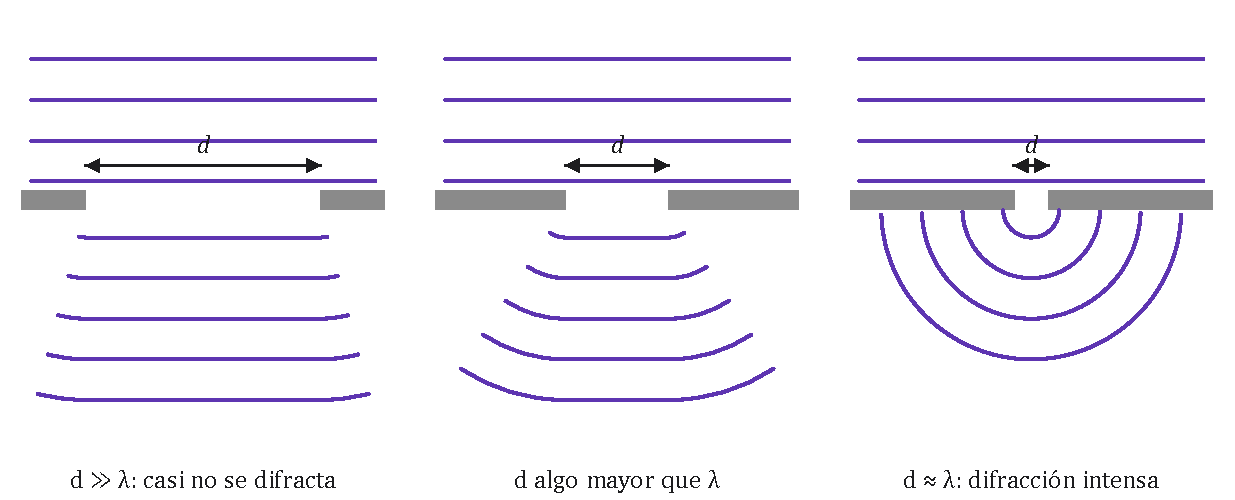
\includegraphics[width=0.95\linewidth]{images/UD2/difraccion}
    \caption{Ondas planas que llegan a una abertura de anchura \(d\). Cuanto más se parece \(d\) a la longitud de onda,
    más se difracta la onda.}
    \label{fig:ond-difraccion}
\end{figure}

La difracción es la razón de que oigamos a alguien que habla detrás de una esquina: las longitudes de onda del sonido (de
centímetros a metros) son parecidas al tamaño de puertas y edificios. La luz, con \(\lambda\) de unos \qty{500}{\nm}, solo
se difracta apreciablemente en rendijas muy estrechas; por eso la difracción es la prueba de que algo se comporta como una
onda.

\section{Reflexión}\label{sec:ond-reflexion}

\begin{definition}[Reflexión]
    La \rojon{reflexión} es el cambio de dirección que sufre una onda al chocar con la superficie de separación con otro
    medio, de forma que vuelve al medio de donde venía. Como no cambia de medio, \textbf{su velocidad, su frecuencia y su
    longitud de onda no cambian}.
\end{definition}

Para describirla se usa la \azuln{normal}, la recta perpendicular a la superficie en el punto de incidencia. El
\azuln{ángulo de incidencia} \(\hat{\imath}\) es el que forma el rayo incidente con la normal, y el \azuln{ángulo de
reflexión} \(\hat r\), el que forma el rayo reflejado con la normal (figura~\ref{fig:ond-reflexion}).

\begin{figure}[H]
    \centering
    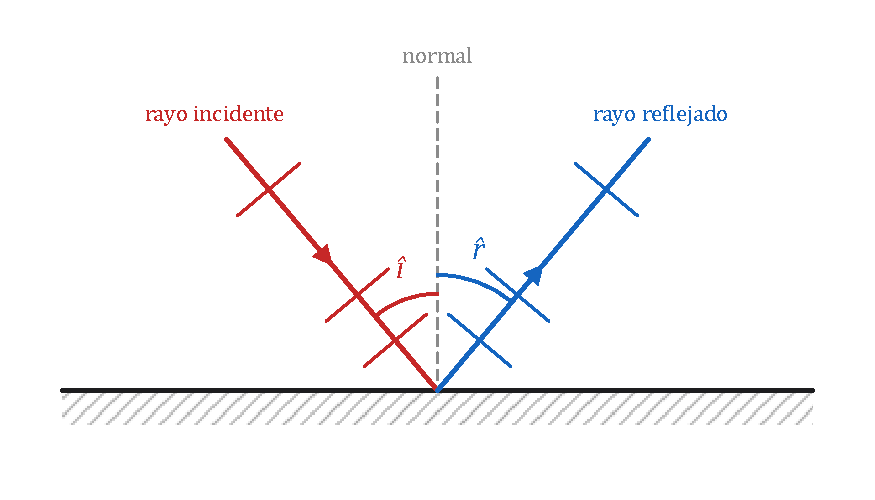
\includegraphics[width=0.52\linewidth]{images/UD2/reflexion}
    \caption{Reflexión de una onda plana. Los segmentos cortos representan los frentes de onda.}
    \label{fig:ond-reflexion}
\end{figure}

\paragraph{Leyes de la reflexión.}
\begin{enumerate}[label=\numberballmDarkTeal]
    \item El rayo incidente, la normal y el rayo reflejado están en el mismo plano.
    \item El ángulo de incidencia es igual al de reflexión: \(\boxed{\hat{\imath} = \hat r}\).
\end{enumerate}
Se deducen con el principio de Huygens: mientras un extremo del frente incidente recorre la distancia que le falta hasta la
superficie, la onda secundaria emitida por el otro extremo recorre la misma distancia en el mismo medio. Los dos triángulos
rectángulos que se forman son iguales y, por tanto, también los ángulos.

\paragraph{Cambio de fase en la reflexión.} Cuando un pulso que viaja por una cuerda llega a un \textbf{extremo fijo}, la
cuerda tira del soporte y, por la tercera ley de Newton, el soporte tira de la cuerda en sentido contrario: el pulso vuelve
\textbf{invertido}, con un cambio de fase de \(\pi\). Si el extremo es \textbf{libre} (por ejemplo, una anilla que desliza
sin rozamiento por una varilla), el pulso vuelve \textbf{sin invertirse} (figura~\ref{fig:ond-reflexion-pulso}).

\begin{figure}[H]
    \centering
    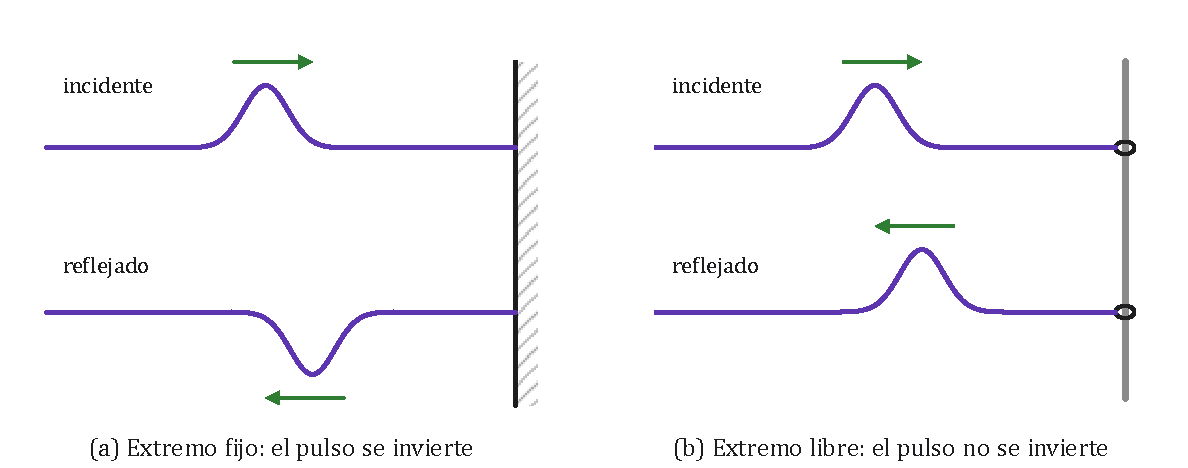
\includegraphics[width=0.88\linewidth]{images/UD2/reflexion_pulso}
    \caption{Reflexión de un pulso en el extremo de una cuerda.}
    \label{fig:ond-reflexion-pulso}
\end{figure}

\section{Refracción}\label{sec:ond-refraccion}

\begin{definition}[Refracción]
    La \rojon{refracción} es el cambio de dirección que sufre una onda al pasar de un medio a otro en el que su velocidad de
    propagación es distinta. La \textbf{frecuencia no cambia} (la impone el foco), pero sí la velocidad y, por tanto, la
    longitud de onda.
\end{definition}

\paragraph{Leyes de la refracción.}
\begin{enumerate}[label=\numberballmDarkTeal]
    \item El rayo incidente, la normal y el rayo refractado están en el mismo plano.
    \item El ángulo de incidencia y el de refracción cumplen la \rojon{ley de Snell}:
    \begin{centeredequation}
        \boxed{\dfrac{\sen\hat{\imath}}{\sen\hat r} = \dfrac{v_1}{v_2}} \label{eq:ond-snell}
    \end{centeredequation}
\end{enumerate}

\begin{figure}[H]
    \centering
    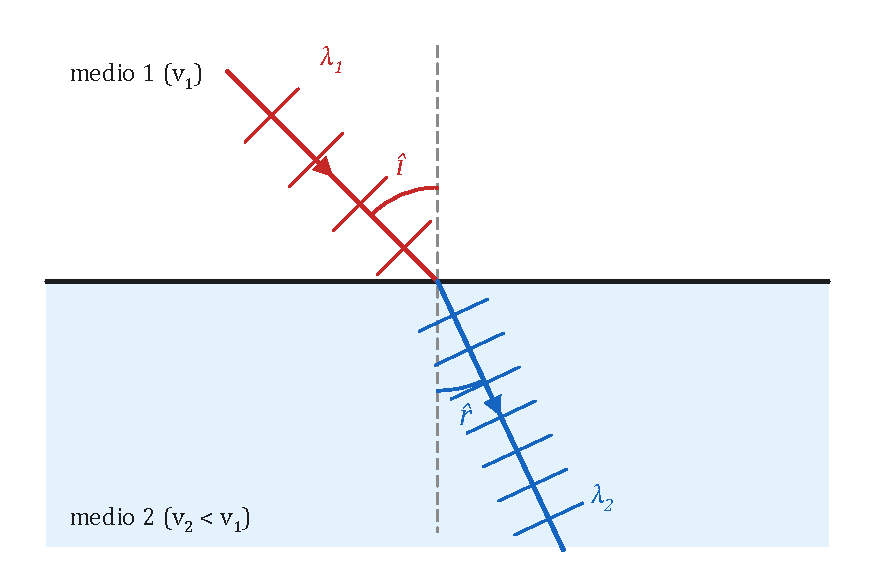
\includegraphics[width=0.52\linewidth]{images/UD2/refraccion}
    \caption{Al entrar en un medio donde va más despacio, la onda se acerca a la normal y sus frentes se juntan
    (\(\lambda_2 < \lambda_1\)).}
    \label{fig:ond-refraccion}
\end{figure}

\paragraph{Deducción con el principio de Huygens.} Un frente plano llega oblicuamente a la superficie. Su extremo \(A\)
toca primero la superficie y emite una onda secundaria hacia el medio 2. En el tiempo \(t\) que tarda el otro extremo en
llegar a la superficie (recorriendo \(v_1 t\)), la onda secundaria de \(A\) avanza \(v_2 t\) en el medio 2. Si \(d\) es la
distancia sobre la superficie entre los dos puntos de llegada, la geometría da \(v_1 t = d\sen\hat{\imath}\) y
\(v_2 t = d\sen\hat r\). Dividiendo, se obtiene la ley de Snell. Si \(v_2 < v_1\), el rayo se acerca a la normal; si
\(v_2 > v_1\), se aleja.

\begin{remark}
    En la reflexión la onda no cambia de medio, \(v_1 = v_2\), y la ley de Snell da \(\sen\hat{\imath} = \sen\hat r\), es
    decir, \(\hat{\imath} = \hat r\): la segunda ley de la reflexión.
\end{remark}

\begin{exercise}
    Un sonido pasa del aire (\qty{340}{\m\per\second}) al agua (\qty{1450}{\m\per\second}) con un ángulo de incidencia de
    \ang{10}. ¿Con qué ángulo se refracta? ¿Qué ocurre si el ángulo de incidencia es mayor de \ang{13.6}?
    \begin{solu}
        \(\sen\hat r = \dfrac{v_2}{v_1}\sen\hat{\imath} = \dfrac{1450}{340}\sen\ang{10} = 0{,}741 \Rightarrow \textcolor{red}{\hat r = \ang{47.8}}\):
        \textcolor{blue}{se aleja mucho de la normal porque en el agua va más deprisa.}

        \textcolor{blue}{El ángulo de refracción llega a \ang{90} cuando \(\sen\hat{\imath} = \dfrac{340}{1450} = 0{,}234\), es decir, \(\hat{\imath} = \ang{13.6}\).}
        \textcolor{red}{Para ángulos mayores no hay onda refractada: el sonido se refleja por completo} \textcolor{blue}{(reflexión total, que estudiaremos en óptica).}
    \end{solu}
\end{exercise}

\section{Polarización}\label{sec:ond-polarizacion}

En una onda transversal que avanza en la dirección del eje \(X\), cada punto puede vibrar en cualquier dirección del plano
\(YZ\). Si la vibración se produce siempre en una misma dirección, decimos que la onda está \rojon{polarizada linealmente}.

Si agitamos de arriba abajo una cuerda que pasa por una rendija vertical, la onda la atraviesa; si la rendija es
horizontal, la onda no pasa (figura~\ref{fig:ond-polarizacion}). Una rendija así actúa como un \azuln{polarizador}: solo
deja pasar la vibración en una dirección.

\begin{figure}[H]
    \centering
    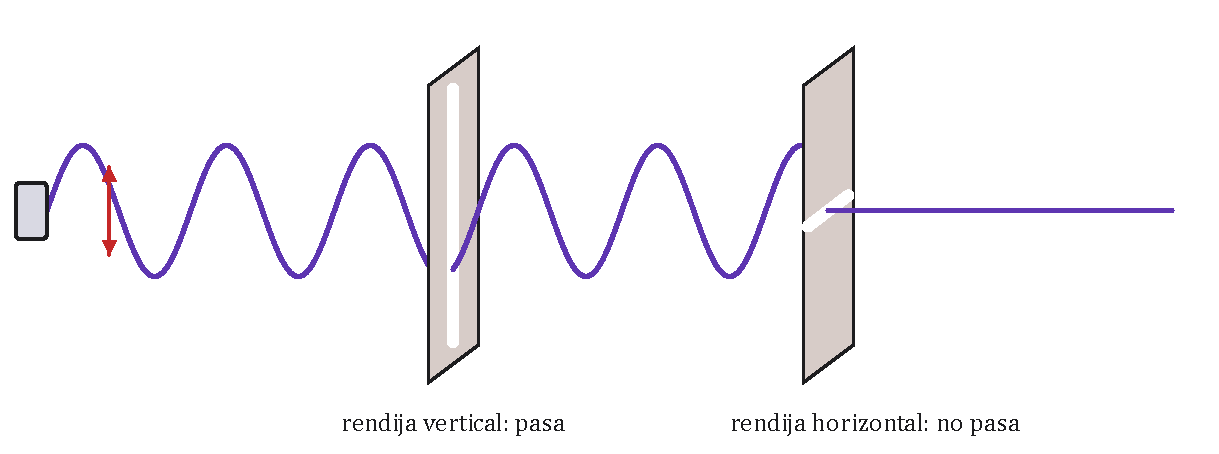
\includegraphics[width=0.9\linewidth]{images/UD2/polarizacion}
    \caption{Una onda que vibra en vertical atraviesa una rendija vertical, pero una rendija horizontal la detiene.}
    \label{fig:ond-polarizacion}
\end{figure}

\begin{remark}
    \textbf{Solo se pueden polarizar las ondas transversales}: en una onda longitudinal la vibración tiene la dirección de
    la propagación y cualquier rendija la deja pasar. Por eso la luz se puede polarizar (es transversal) y el sonido no.
    Las gafas de sol polarizadas y las pantallas LCD aprovechan este fenómeno.
\end{remark}

\section{Efecto Doppler}\label{sec:ond-doppler}

Cuando una ambulancia se acerca, su sirena suena más aguda, y al alejarse, más grave. El \rojon{efecto Doppler} es el
cambio de la frecuencia percibida por un observador cuando el foco, el observador o ambos se mueven el uno respecto del
otro. Llamemos \(\nu\) a la frecuencia emitida, \(\nu'\) a la percibida, \(v\) a la velocidad del sonido,
\(v_O\) a la del observador y \(v_F\) a la del foco.

\paragraph{Observador en movimiento, foco quieto.} Si el observador se acerca al foco, encuentra las ondas a una velocidad
relativa \(v + v_O\). La longitud de onda no cambia, \(\lambda = v/\nu\), así que le llegan más frentes por segundo:
\begin{equation*}
    \nu' = \dfrac{v + v_O}{\lambda} = \nu\,\dfrac{v + v_O}{v} \qquad \text{(si se aleja: } v - v_O\text{)}
\end{equation*}

\paragraph{Foco en movimiento, observador quieto.} Ahora los frentes no son concéntricos: el foco «persigue» a las ondas
que emite hacia delante (figura~\ref{fig:ond-doppler}). Mientras un frente avanza \(\lambda = vT\), el foco avanza
\(v_F T\), y la distancia entre frentes delante del foco es \(\lambda' = (v - v_F)\,T\). El observador que tiene delante
percibe:
\begin{equation*}
    \nu' = \dfrac{v}{\lambda'} = \nu\,\dfrac{v}{v - v_F} \qquad \text{(si el foco se aleja: } v + v_F\text{)}
\end{equation*}

\begin{figure}[H]
    \centering
    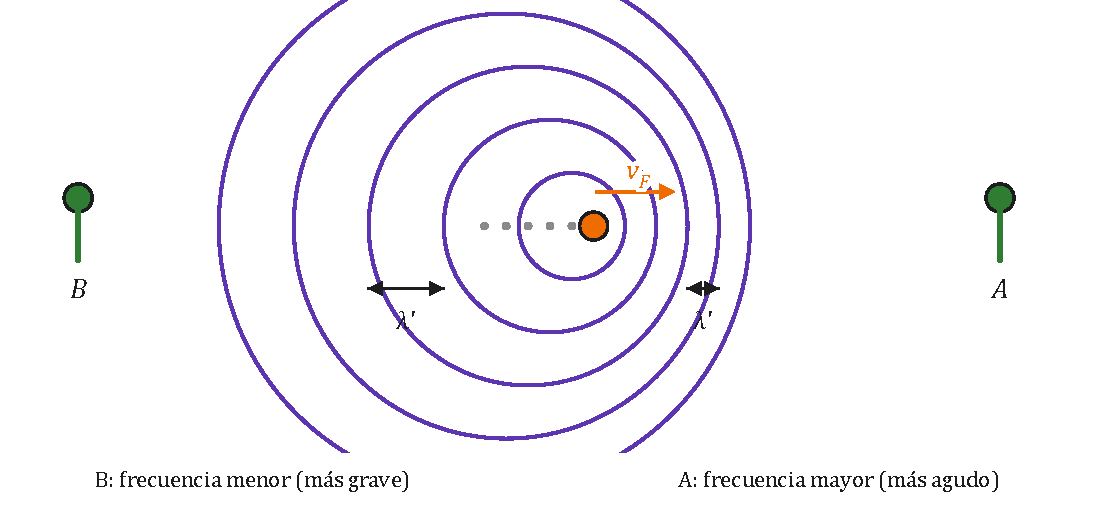
\includegraphics[width=0.72\linewidth]{images/UD2/doppler}
    \caption{Frentes de onda emitidos por un foco que se mueve hacia la derecha. El observador \(A\) recibe los frentes más
    juntos (frecuencia mayor) y el \(B\), más separados (frecuencia menor).}
    \label{fig:ond-doppler}
\end{figure}

\paragraph{Caso general.} Juntando los dos efectos:
\begin{centeredequation}
    \boxed{\nu' = \nu\,\dfrac{v \pm v_O}{v \mp v_F}} \label{eq:ond-doppler}
\end{centeredequation}
\begin{itemize}
    \item Se usan los \textbf{signos de arriba} (\(+v_O\) en el numerador, \(-v_F\) en el denominador) cuando el observador o
    el foco se mueven \textbf{acercándose} al otro.
    \item Se usan los \textbf{signos de abajo} cuando se mueven \textbf{alejándose}.
\end{itemize}
Comprobación rápida: al acercarse, la frecuencia percibida debe salir \emph{mayor} que la emitida; al alejarse, menor.

\begin{exercise}
    Una ambulancia circula a \qty{90}{\km\per\hour} con la sirena encendida a \qty{700}{\hertz}. ¿Qué frecuencia oye un
    peatón parado cuando la ambulancia se acerca? ¿Y cuando se aleja? (\(v = \qty{340}{\m\per\second}\)).
    \begin{solu}
        \textcolor{blue}{\(v_F = \qty{25}{\m\per\second}\), \(v_O = 0\).}

        Se acerca: \(\nu' = 700\cdot\dfrac{340}{340 - 25} = \textcolor{red}{\qty{756}{\hertz}}\).
        Se aleja: \(\nu' = 700\cdot\dfrac{340}{340 + 25} = \textcolor{red}{\qty{652}{\hertz}}\).

        \textcolor{blue}{Al pasar a su lado, el peatón oye bajar el tono unos \qty{100}{\hertz}.}
    \end{solu}
\end{exercise}

\begin{exercise}
    Un coche patrulla circula a \qty{108}{\km\per\hour} con la sirena a \qty{600}{\hertz} y se acerca a un ciclista que va
    hacia él a \qty{72}{\km\per\hour}. ¿Qué frecuencia oye el ciclista? ¿Y después de cruzarse?
    \begin{solu}
        \textcolor{blue}{\(v_F = \qty{30}{\m\per\second}\), \(v_O = \qty{20}{\m\per\second}\). Antes de cruzarse, los dos se acercan:}
        \(\nu' = 600\cdot\dfrac{340 + 20}{340 - 30} = \textcolor{red}{\qty{697}{\hertz}}\).

        \textcolor{blue}{Después, los dos se alejan:} \(\nu' = 600\cdot\dfrac{340 - 20}{340 + 30} = \textcolor{red}{\qty{519}{\hertz}}\).
    \end{solu}
\end{exercise}

\begin{remark}
    El efecto Doppler tiene muchas aplicaciones: los radares de tráfico miden la velocidad de los coches con el cambio de
    frecuencia de las ondas que rebotan en ellos; las ecografías Doppler miden la velocidad de la sangre; y en astronomía
    el desplazamiento de la luz de las galaxias hacia el rojo indica que se alejan de nosotros (expansión del universo).
\end{remark}

\section{Resumen de fórmulas}\label{sec:ond-resumen}

\begin{table}[H]
    \centering
    \caption{Fórmulas principales del movimiento ondulatorio}
    \vspace{-5pt}
    \begin{tabular}{@{}lL{10cm}@{}}
        \toprule
        \textbf{Magnitud} & \textbf{Expresión} \\
        \midrule
        Relaciones básicas & \(\lambda = vT = v/\nu\), \quad \(k = 2\pi/\lambda\), \quad \(\omega = 2\pi\nu\), \quad \(v = \omega/k\) \\[3pt]
        Ecuación de onda & \(y = A\sen(\omega t \mp kx + \varphi_0)\) \quad (\(-\): hacia \(+X\); \(+\): hacia \(-X\)) \\[3pt]
        Velocidad de vibración & \(v_y = A\omega\cos(\omega t - kx + \varphi_0)\), \quad \(v_{y,\text{máx}} = A\omega\) \\[3pt]
        Puntos en fase / oposición & \(\Delta x = n\lambda\) \quad / \quad \(\Delta x = (2n - 1)\lambda/2\) \\[3pt]
        Intensidad & \(I = P/S\), \quad \(I = P/(4\pi r^2)\), \quad \(I_1/I_2 = r_2^2/r_1^2 = A_1^2/A_2^2\) \\[3pt]
        Absorción & \(I = I_0\,e^{-\beta x}\) \\[3pt]
        Nivel de intensidad sonora & \(\beta = 10\log(I/I_0)\), \quad \(I_0 = \qty{e-12}{\watt\per\square\m}\) \\[3pt]
        Interferencia (focos en fase) & máximo: \(x_2 - x_1 = n\lambda\); \quad mínimo: \(x_2 - x_1 = (2n - 1)\lambda/2\) \\[3pt]
        Onda estacionaria & \(y = 2A\sen(kx)\cos(\omega t)\) \\[3pt]
        Nodos y vientres & nodos en \(x = n\lambda/2\); \quad vientres en \(x = (2n - 1)\lambda/4\) \\[3pt]
        Armónicos & dos extremos fijos: \(\nu_n = n\,v/2L\); \quad un extremo libre: \(\nu = (2n - 1)\,v/4L\) \\[3pt]
        Ley de Snell & \(\sen\hat{\imath}/\sen\hat r = v_1/v_2\) \\[3pt]
        Efecto Doppler & \(\nu' = \nu\,(v \pm v_O)/(v \mp v_F)\) \quad (signos de arriba: acercándose) \\
        \bottomrule
    \end{tabular}
    \label{tab:ond-resumen}
\end{table}

\section{Prácticas de laboratorio}\label{sec:ond-practicas}

\subsection{Práctica 1: ondas estacionarias en una cuerda}\label{subsec:ond-practica-melde}

\noindent\begin{minipage}[t]{0.58\linewidth}
\textbf{Objetivo.} Producir ondas estacionarias en una cuerda (experiencia de Melde), comprobar que solo aparecen ciertos
modos de vibración y medir la velocidad de las ondas.

\textbf{Material.} Vibrador de frecuencia conocida (o generador de funciones con un excitador), cuerda o hilo elástico,
polea con soporte, portapesas y pesas, regla, balanza.

\textbf{Procedimiento.}
\begin{enumerate}[label=\numberballmDarkTeal]
    \item Mide la masa y la longitud de un trozo largo de cuerda para calcular \(\mu = m/l\).
    \item Monta el dispositivo de la figura~\ref{fig:ond-practica-melde}: la cuerda va del vibrador a la polea y del otro
    extremo cuelgan las pesas. La tensión es \(T = m g\).
    \item Enciende el vibrador y cambia la masa colgada (o la frecuencia) hasta que se vea una onda estacionaria nítida.
    Cuenta los husos \(n\) y mide la longitud \(L\) entre el vibrador y la polea.
    \item Repite para varios valores de \(n\).
\end{enumerate}
\end{minipage}\hfill
\begin{minipage}[t]{0.38\linewidth}
    \vspace{0pt}
    \centering
    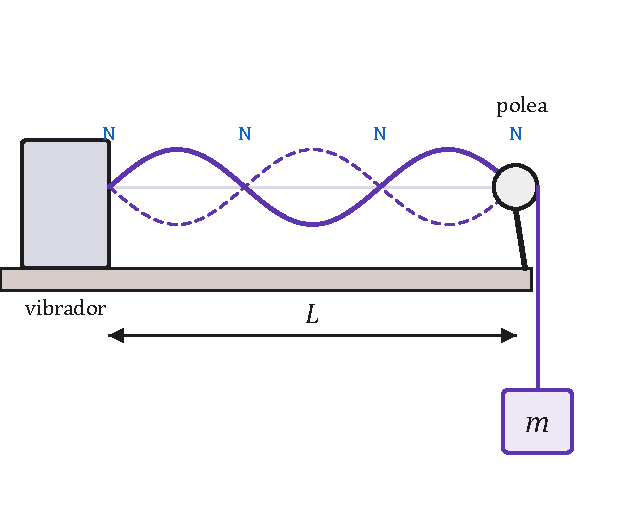
\includegraphics[width=\linewidth]{images/UD2/practica_melde}
    \captionof{figure}{Montaje de la experiencia de Melde.}
    \label{fig:ond-practica-melde}
\end{minipage}

\begin{table}[H]
    \centering
    \caption{Datos de la práctica de ondas estacionarias}
    \vspace{-5pt}
    \begin{tabular}{@{}C{2cm}C{1.6cm}C{2cm}C{2.4cm}C{2.4cm}C{2.4cm}@{}}
        \toprule
        \textbf{\(m\) (\unit{\kg})} & \textbf{\(n\)} & \textbf{\(L\) (\unit{\m})} & \textbf{\(\lambda = 2L/n\) (\unit{\m})} & \textbf{\(v = \lambda\nu\) (\unit{\m\per\second})} & \textbf{\(v = \sqrt{T/\mu}\) (\unit{\m\per\second})} \\
        \midrule
        \rule{0pt}{18pt} & & & & & \\ \midrule[0.3pt]
        \rule{0pt}{18pt} & & & & & \\ \midrule[0.3pt]
        \rule{0pt}{18pt} & & & & & \\
        \bottomrule
    \end{tabular}
    \label{tab:ond-practica-melde}
\end{table}

\textbf{Cálculos.} Con los dos extremos fijos (el vibrador y la polea son casi nodos), \(\lambda = 2L/n\) y
\(v = \lambda\nu\). Compara ese valor con el teórico \(v = \sqrt{T/\mu}\).

\textbf{Cuestiones.}
\begin{enumerate}[label=\letraminuscula]
    \item Si con una masa de \qty{200}{\g} y \(\mu = \qty{2}{\g\per\m}\) la velocidad teórica es \qty{31.3}{\m\per\second},
    ¿cuántos husos esperas ver con \(\nu = \qty{50}{\hertz}\) y \(L = \qty{1.25}{\m}\)?
    \item ¿Qué le pasa al número de husos si aumentas la masa colgada? Explícalo.
    \item ¿Por qué entre dos modos de vibración la cuerda apenas se mueve?
\end{enumerate}

\subsection{Práctica 2: velocidad del sonido con un tubo de resonancia}\label{subsec:ond-practica-tubo}

\noindent\begin{minipage}[t]{0.64\linewidth}
\textbf{Objetivo.} Medir la velocidad del sonido en el aire usando la resonancia de una columna de aire.

\textbf{Material.} Tubo de vidrio o de plástico de \qty{1}{\m} aproximadamente, probeta alta o recipiente con agua (para
variar el nivel), diapasones de frecuencia conocida (o una aplicación de móvil que emita un tono puro), regla y termómetro.

\textbf{Fundamento.} El tubo, cerrado abajo por el agua, se comporta como una cuerda con un extremo fijo y otro libre: en
la superficie del agua hay un nodo y en la boca del tubo, un vientre. La primera resonancia se produce cuando la columna de
aire mide \(L_1 = \lambda/4\) y la segunda cuando mide \(L_2 = 3\lambda/4\); entre las dos hay \(\lambda/2\).

\textbf{Procedimiento.}
\begin{enumerate}[label=\numberballmDarkTeal]
    \item Golpea el diapasón y sostenlo sobre la boca del tubo (figura~\ref{fig:ond-practica-tubo}).
    \item Sube o baja el tubo (o el nivel del agua) hasta que el sonido se refuerce claramente. Mide \(L_1\).
    \item Sigue alargando la columna de aire hasta la siguiente resonancia y mide \(L_2\).
    \item Repite con otros diapasones y anota la temperatura del laboratorio.
\end{enumerate}
\end{minipage}\hfill
\begin{minipage}[t]{0.32\linewidth}
    \vspace{0pt}
    \centering
    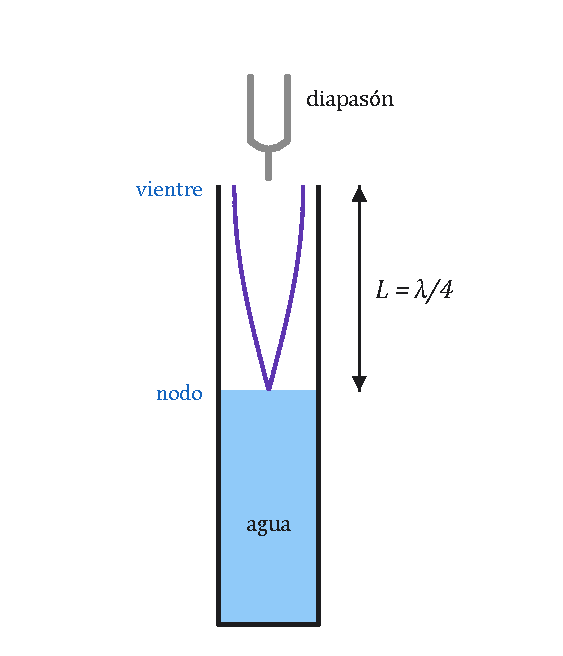
\includegraphics[width=0.85\linewidth]{images/UD2/practica_tubo}
    \captionof{figure}{Columna de aire en resonancia.}
    \label{fig:ond-practica-tubo}
\end{minipage}

\begin{table}[H]
    \centering
    \caption{Datos de la práctica del tubo de resonancia}
    \vspace{-5pt}
    \begin{tabular}{@{}C{2.2cm}C{2.2cm}C{2.2cm}C{3.2cm}C{3cm}@{}}
        \toprule
        \textbf{\(\nu\) (\unit{\hertz})} & \textbf{\(L_1\) (\unit{\m})} & \textbf{\(L_2\) (\unit{\m})} & \textbf{\(\lambda = 2(L_2 - L_1)\) (\unit{\m})} & \textbf{\(v = \lambda\nu\) (\unit{\m\per\second})} \\
        \midrule
        \rule{0pt}{18pt} & & & & \\ \midrule[0.3pt]
        \rule{0pt}{18pt} & & & & \\ \midrule[0.3pt]
        \rule{0pt}{18pt} & & & & \\
        \bottomrule
    \end{tabular}
    \label{tab:ond-practica-tubo}
\end{table}

\textbf{Cálculos.} Usa \(\lambda = 2(L_2 - L_1)\): así no influye que el vientre esté en realidad un poco por encima de la
boca del tubo. Calcula \(v = \lambda\nu\) y su valor medio.

\textbf{Cuestiones.}
\begin{enumerate}[label=\letraminuscula]
    \item Compara tu resultado con el teórico \(v = \sqrt{\gamma R T/M}\) a la temperatura del laboratorio
    (\(\gamma = 1{,}4\); \(M = \qty{0.029}{\kg\per\mol}\)) y calcula el error relativo.
    \item Calcula \(4L_1\) y compáralo con \(\lambda\). ¿Por qué no coinciden exactamente?
    \item Con un diapasón de \qty{512}{\hertz}, ¿a qué longitudes de la columna de aire esperas las dos primeras resonancias?
\end{enumerate}


    \newpage

    %! Unidad 2 — Movimiento ondulatorio: ejercicios finales (adaptados de la fuente, con datos cambiados y resueltos)

\section{Ejercicios}\label{sec:ond-ejercicios}

\subsection{Ecuación de una onda}

\begin{exercise}
    Una onda armónica de \qty{50}{\hertz} y \qty{0.4}{\m} de amplitud se propaga a \qty{20}{\m\per\second} en el sentido
    positivo del eje \(X\). En el instante inicial, la elongación del origen es máxima y positiva. Calcula:
    \begin{enumerate}[label=\letraminuscula]
        \item La ecuación de la onda.
        \item La diferencia de fase entre dos puntos separados \qty{0.3}{\m}.
        \item La velocidad y la aceleración máximas de un punto del medio.
    \end{enumerate}
    \begin{solu}
        \textcolor{blue}{\(\omega = 2\pi\nu = 100\pi\ \unit{\radian\per\second}\); \(k = \omega/v = 5\pi\ \unit{\per\m}\).}
        \begin{enumerate}[label=\letraminuscula]
            \item \textcolor{blue}{En \(x = 0\), \(t = 0\): \(0{,}4 = 0{,}4\sen\varphi_0 \Rightarrow \varphi_0 = \pi/2\).}
            \(\textcolor{red}{y = 0{,}4\sen\!\left(100\pi t - 5\pi x + \dfrac{\pi}{2}\right)\ \text{(SI)}}\)
            \item \(\Delta\varphi = k\,\Delta x = 5\pi\cdot 0{,}3 = \textcolor{red}{1{,}5\pi\ \unit{\radian}}\).
            \item \(v_{\text{máx}} = A\omega = 40\pi = \textcolor{red}{\qty{126}{\m\per\second}}\);
            \(a_{\text{máx}} = A\omega^2 = 0{,}4\,(100\pi)^2 = \textcolor{red}{\qty{3.95e4}{\m\per\second\squared}}\).
        \end{enumerate}
    \end{solu}
\end{exercise}

\begin{exercise}
    Un foco \(F\) vibra con un m.a.s. de \qty{6}{\cm} de amplitud y \qty{25}{\hertz}, y la perturbación se propaga a
    \qty{5}{\m\per\second}. En \(t = 0\) el foco está en su posición de equilibrio.
    \begin{enumerate}[label=\letraminuscula]
        \item Escribe la ecuación de la onda con la función seno y con la función coseno.
        \item Calcula la velocidad de vibración de un punto situado a \qty{2}{\m} del foco \qty{8}{\second} después de empezar.
    \end{enumerate}
    \begin{solu}
        \textcolor{blue}{\(\omega = 50\pi\ \unit{\radian\per\second}\); \(k = \omega/v = 10\pi\ \unit{\per\m}\); \(A = \qty{0.06}{\m}\).}
        \begin{enumerate}[label=\letraminuscula]
            \item \(\textcolor{red}{y = 0{,}06\sen(50\pi t - 10\pi x)}\) \(\;=\; \textcolor{red}{0{,}06\cos\!\left(50\pi t - 10\pi x - \dfrac{\pi}{2}\right)}\) (SI).
            \item \textcolor{blue}{La onda llega a \(x = \qty{2}{\m}\) en \(2/5 = \qty{0.4}{\second}\), así que en \(t = \qty{8}{\second}\) ese punto ya vibra.}
            \(v_y = 0{,}06\cdot 50\pi\cos(400\pi - 20\pi) = 3\pi\cos(380\pi) = \textcolor{red}{3\pi \approx \qty{9.42}{\m\per\second}}\)
            \textcolor{blue}{(pasa por el equilibrio con la velocidad máxima).}
        \end{enumerate}
    \end{solu}
\end{exercise}

\begin{exercise}
    Por una cuerda se propaga la onda \(y = 15\sen(8x + 120t)\), con \(x\) e \(y\) en centímetros y \(t\) en segundos.
    Calcula:
    \begin{enumerate}[label=\letraminuscula]
        \item La velocidad de propagación y su sentido.
        \item La velocidad transversal de un punto situado en \(x = \qty{20}{\cm}\) en \(t = \qty{4}{\second}\).
        \item La diferencia de fase, en un instante dado, entre dos puntos separados \qty{0.5}{\cm}.
        \item La distancia entre dos puntos cuya diferencia de fase es de \ang{45}.
    \end{enumerate}
    \begin{solu}
        \textcolor{blue}{\(k = \qty{8}{\per\cm}\), \(\omega = \qty{120}{\radian\per\second}\).}
        \begin{enumerate}[label=\letraminuscula]
            \item \(v = \dfrac{\omega}{k} = \textcolor{red}{\qty{15}{\cm\per\second}}\), \textcolor{red}{hacia las \(x\) negativas} \textcolor{blue}{(\(kx\) y \(\omega t\) tienen el mismo signo).}
            \item \(v_y = 15\cdot 120\cos(8\cdot 20 + 120\cdot 4) = 1800\cos(640) = \textcolor{red}{\qty{1140}{\cm\per\second} = \qty{11.4}{\m\per\second}}\).
            \item \(\Delta\varphi = k\,\Delta x = 8\cdot 0{,}5 = \textcolor{red}{\qty{4}{\radian}}\).
            \item \(\Delta x = \dfrac{\Delta\varphi}{k} = \dfrac{\pi/4}{8} = \textcolor{red}{\qty{0.098}{\cm}}\).
        \end{enumerate}
    \end{solu}
\end{exercise}

\begin{exercise}
    Una onda de \qty{400}{\hertz} se propaga a \qty{320}{\m\per\second}. ¿Qué distancia separa dos puntos con una diferencia de
    fase de \ang{60}? ¿Qué diferencia de fase hay entre dos elongaciones de un mismo punto separadas \qty{2}{\ms}?
    \begin{solu}
        \textcolor{blue}{\(\lambda = v/\nu = \qty{0.8}{\m}\).}
        \(\Delta x = \dfrac{\pi/3}{2\pi}\,\lambda = \dfrac{\lambda}{6} = \textcolor{red}{\qty{0.133}{\m}}\).

        \(\Delta\varphi = \omega\,\Delta t = 2\pi\cdot 400\cdot 0{,}002 = \textcolor{red}{1{,}6\pi\ \unit{\radian}}\).
    \end{solu}
\end{exercise}

\begin{exercise}
    La ecuación de una onda es \(y = 20\sen(0{,}5t - \pi x)\) (SI). ¿Cuándo tiene velocidad máxima por primera vez un punto
    situado a \qty{4}{\m} del foco?
    \begin{solu}
        \textcolor{blue}{\(v = \omega/k = 0{,}5/\pi\ \unit{\m\per\second}\): la onda tarda \(t = x/v = 4\pi/0{,}5 = 8\pi\ \unit{\second}\) en llegar.
        La velocidad de vibración, \(v_y = A\omega\cos(0{,}5t - \pi x)\), es máxima cuando la fase es \(0\) (o \(n\pi\)):}
        \[ 0{,}5t - 4\pi = 0 \;\Rightarrow\; \textcolor{red}{t = 8\pi \approx \qty{25.1}{\second}} \]
        \textcolor{blue}{Justo al llegarle la onda, pasa por el equilibrio con velocidad máxima. Se repite cada medio período, \(T/2 = 2\pi\ \unit{\second}\).}
    \end{solu}
\end{exercise}

\begin{exercise}
    Dada la onda \(y = 0{,}04\sen 2\pi(5t - 0{,}25x)\) (SI), calcula el período, la frecuencia, la longitud de onda, la
    velocidad de propagación y la velocidad máxima de vibración de un punto.
    \begin{solu}
        \textcolor{blue}{Comparando con \(y = A\sen 2\pi\left(\dfrac{t}{T} - \dfrac{x}{\lambda}\right)\):}
        \(\nu = \textcolor{red}{\qty{5}{\hertz}}\); \(T = \textcolor{red}{\qty{0.2}{\second}}\); \(\lambda = 1/0{,}25 = \textcolor{red}{\qty{4}{\m}}\);
        \(v = \lambda\nu = \textcolor{red}{\qty{20}{\m\per\second}}\); \(v_{y,\text{máx}} = A\omega = 0{,}04\cdot 10\pi = \textcolor{red}{\qty{1.26}{\m\per\second}}\).
    \end{solu}
\end{exercise}

\begin{exercise}
    Una onda armónica de \qty{200}{\hertz}, \qty{400}{\m\per\second} y \qty{10}{\cm} de amplitud avanza en el sentido positivo
    del eje \(X\). En el instante inicial, la partícula del origen está en su elongación máxima positiva.
    \begin{enumerate}[label=\letraminuscula]
        \item Escribe la ecuación de la onda.
        \item Calcula la diferencia de fase entre dos puntos separados \qty{3}{\m}.
        \item ¿Cuál es la velocidad máxima de vibración?
    \end{enumerate}
    \begin{solu}
        \textcolor{blue}{\(\omega = 400\pi\ \unit{\radian\per\second}\); \(k = \omega/v = \pi\ \unit{\per\m}\); \(\varphi_0 = \pi/2\).}
        \begin{enumerate}[label=\letraminuscula]
            \item \(\textcolor{red}{y = 0{,}1\sen\!\left(400\pi t - \pi x + \dfrac{\pi}{2}\right)\ \text{(SI)}}\)
            \item \(\Delta\varphi = \pi\cdot 3 = \textcolor{red}{3\pi\ \unit{\radian}}\): \textcolor{blue}{están en oposición de fase (\(\lambda = \qty{2}{\m}\) y los separa \(1{,}5\lambda\)).}
            \item \(v_{\text{máx}} = A\omega = 0{,}1\cdot 400\pi = \textcolor{red}{\qty{126}{\m\per\second}}\).
        \end{enumerate}
    \end{solu}
\end{exercise}

\begin{exercise}
    Escribe la ecuación de una onda de \qty{20}{\cm} de amplitud y \qty{5}{\hertz} que avanza hacia la derecha a
    \qty{10}{\m\per\second}, sabiendo que en \(t = \qty{1}{\second}\) la partícula situada a \qty{1}{\m} del origen alcanza
    su elongación máxima positiva. ¿En qué instantes tiene esa partícula aceleración máxima?
    \begin{solu}
        \textcolor{blue}{\(\omega = 10\pi\ \unit{\radian\per\second}\); \(k = \omega/v = \pi\ \unit{\per\m}\). En \(x = 1\), \(t = 1\) la fase debe valer \(\pi/2 + 2n\pi\):}
        \[ 10\pi - \pi + \varphi_0 = \dfrac{\pi}{2} + 2n\pi \;\Rightarrow\; \varphi_0 = \dfrac{3\pi}{2}\ \text{(tomando } n = 5\text{)} \]
        \(\textcolor{red}{y = 0{,}2\sen\!\left(10\pi t - \pi x + \dfrac{3\pi}{2}\right)\ \text{(SI)}}\)

        \textcolor{blue}{La aceleración es máxima en los extremos, cuando \(10\pi t - \pi + \dfrac{3\pi}{2} = \dfrac{\pi}{2} + n\pi\), es decir, \(10\pi t = n\pi\):}
        \(\textcolor{red}{t = 0{,}1\,n\ \unit{\second}}\) \textcolor{blue}{(cada medio período, a partir de \(t = \qty{0.1}{\second}\), que es cuando le llega la onda).}
    \end{solu}
\end{exercise}

\begin{exercise}
    Una piedra cae en un estanque y produce una onda que tarda \qty{4}{\second} en recorrer \qty{8}{\m}. Si la distancia
    entre dos crestas consecutivas es de \qty{40}{\cm}, calcula la velocidad de propagación, la frecuencia y la pulsación.
    \begin{solu}
        \(v = \dfrac{8}{4} = \textcolor{red}{\qty{2}{\m\per\second}}\); \(\nu = \dfrac{v}{\lambda} = \dfrac{2}{0{,}4} = \textcolor{red}{\qty{5}{\hertz}}\);
        \(\omega = 2\pi\nu = \textcolor{red}{10\pi\ \unit{\radian\per\second}}\).
    \end{solu}
\end{exercise}

\begin{exercise}
    Si se triplica la longitud de onda de una onda sin cambiar su frecuencia, ¿cómo varía su velocidad de propagación? ¿Y la
    velocidad máxima de vibración de las partículas del medio?
    \begin{solu}
        \(v = \lambda\nu\): \textcolor{red}{la velocidad de propagación se triplica} \textcolor{blue}{(para eso habría que cambiar de medio)}.
        \(v_{y,\text{máx}} = A\omega = 2\pi\nu A\) \textcolor{red}{no cambia}: \textcolor{blue}{solo depende de la amplitud y de la frecuencia.}
    \end{solu}
\end{exercise}

\begin{exercise}
    Una onda en la superficie del agua tiene \qty{8}{\hertz}, \qty{4}{\cm} de longitud de onda, \qty{2}{\cm} de amplitud y
    fase inicial nula.
    \begin{enumerate}[label=\letraminuscula]
        \item Escribe su ecuación.
        \item Calcula la distancia mínima entre dos puntos cuyas fases difieren \(\pi/3\) rad.
        \item ¿A qué altura está un corcho situado a \qty{15}{\cm} del foco en \(t = \qty{1.5}{\second}\)?
    \end{enumerate}
    \begin{solu}
        \textcolor{blue}{\(\omega = 16\pi\ \unit{\radian\per\second}\); \(k = 2\pi/4 = \pi/2\ \unit{\per\cm}\).}
        \begin{enumerate}[label=\letraminuscula]
            \item \(\textcolor{red}{y = 2\sen\!\left(16\pi t - \dfrac{\pi}{2}x\right)}\) (\(x\), \(y\) en cm; \(t\) en s).
            \item \(\Delta x = \dfrac{\lambda}{6} = \textcolor{red}{\qty{0.67}{\cm}}\).
            \item \(y = 2\sen(24\pi - 7{,}5\pi) = 2\sen(16{,}5\pi) = \textcolor{red}{\qty{2}{\cm}}\): \textcolor{blue}{está en una cresta.}
        \end{enumerate}
    \end{solu}
\end{exercise}

\begin{exercise}
    Dada la onda \(y = 0{,}5\sen 2\pi(4t - 0{,}5x)\) (SI), halla el período, la frecuencia, la longitud de onda, la velocidad de
    propagación y la amplitud. Escribe la ecuación de una onda igual que se propague en sentido contrario.
    \begin{solu}
        \(T = \textcolor{red}{\qty{0.25}{\second}}\); \(\nu = \textcolor{red}{\qty{4}{\hertz}}\); \(\lambda = \textcolor{red}{\qty{2}{\m}}\);
        \(v = \lambda\nu = \textcolor{red}{\qty{8}{\m\per\second}}\); \(A = \textcolor{red}{\qty{0.5}{\m}}\).

        \textcolor{red}{\(y = 0{,}5\sen 2\pi(4t + 0{,}5x)\)}.
    \end{solu}
\end{exercise}

\begin{exercise}
    El período de una onda transversal en una cuerda es de \qty{4}{\ms}. Dos puntos consecutivos cuya diferencia de fase es
    \(\pi/2\) rad están separados \qty{15}{\cm}. Calcula la longitud de onda y la velocidad de propagación.
    \begin{solu}
        \textcolor{blue}{Una diferencia de fase de \(\pi/2\) corresponde a \(\lambda/4\):} \(\lambda = 4\cdot 0{,}15 = \textcolor{red}{\qty{0.6}{\m}}\);
        \(v = \dfrac{\lambda}{T} = \dfrac{0{,}6}{0{,}004} = \textcolor{red}{\qty{150}{\m\per\second}}\).
    \end{solu}
\end{exercise}

\subsection{Energía, intensidad y sonido}

\begin{exercise}
    Un altavoz emite con una potencia de \qty{300}{\watt}. ¿Qué nivel de intensidad sonora hay a \qty{5}{\m}? ¿Y a \qty{10}{\m}?
    \begin{solu}
        \(I_5 = \dfrac{300}{4\pi\cdot 25} = \qty{0.955}{\watt\per\square\m} \Rightarrow \beta = 10\log\dfrac{0{,}955}{10^{-12}} = \textcolor{red}{\qty{119.8}{\deci\bel}}\).

        \(I_{10} = \dfrac{I_5}{4} = \qty{0.239}{\watt\per\square\m} \Rightarrow \beta = \textcolor{red}{\qty{113.8}{\deci\bel}}\)
        \textcolor{blue}{(al doblar la distancia el nivel baja \qty{6}{\deci\bel}).}
    \end{solu}
\end{exercise}

\begin{exercise}
    En un partido, un espectador canta un gol con un nivel de \qty{45}{\deci\bel}. ¿Qué nivel se alcanzaría si lo cantaran a la
    vez y con la misma intensidad 2000 espectadores? ¿Cuántos harían falta para llegar a \qty{80}{\deci\bel}?
    \begin{solu}
        \textcolor{blue}{Las intensidades se suman: \(I = N I_1\), así que \(\beta = \beta_1 + 10\log N\).}

        \(\beta = 45 + 10\log 2000 = \textcolor{red}{\qty{78}{\deci\bel}}\).
        \textcolor{blue}{Para \qty{80}{\deci\bel}:} \(10\log N = 35 \Rightarrow N = 10^{3{,}5} \approx \textcolor{red}{3162}\) espectadores.
    \end{solu}
\end{exercise}

\begin{exercise}
    Una ventana de \qty{2}{\square\m} da a una calle con un nivel de ruido de \qty{70}{\deci\bel}. ¿Qué potencia sonora entra
    por la ventana abierta?
    \begin{solu}
        \(I = 10^{-12}\cdot 10^{7} = \qty{e-5}{\watt\per\square\m}\); \(P = I S = \textcolor{red}{\qty{2e-5}{\watt}}\).
    \end{solu}
\end{exercise}

\begin{exercise}
    Se duplica la frecuencia de una onda sonora y se triplica su amplitud. ¿Por cuánto se multiplica su intensidad? ¿Cuánto
    aumenta su nivel de intensidad sonora?
    \begin{solu}
        \textcolor{blue}{\(I \propto \nu^2 A^2\):} \(\dfrac{I'}{I} = 2^2\cdot 3^2 = \textcolor{red}{36}\).
        \(\Delta\beta = 10\log 36 = \textcolor{red}{\qty{15.6}{\deci\bel}}\).
    \end{solu}
\end{exercise}

\begin{exercise}
    Un foco puntual de \qty{20}{\watt} emite sonido por igual en todas direcciones. Calcula la intensidad y el nivel de
    intensidad sonora a \qty{5}{\m} del foco.
    \begin{solu}
        \(I = \dfrac{20}{4\pi\cdot 25} = \textcolor{red}{\qty{0.0637}{\watt\per\square\m}}\);
        \(\beta = 10\log\dfrac{0{,}0637}{10^{-12}} = \textcolor{red}{\qty{108}{\deci\bel}}\).
    \end{solu}
\end{exercise}

\begin{exercise}
    La intensidad de un sonido es cuatro veces la de otro. ¿Qué diferencia hay entre sus niveles de intensidad sonora?
    \begin{solu}
        \(\Delta\beta = 10\log\dfrac{I_1}{I_2} = 10\log 4 = \textcolor{red}{\qty{6.0}{\deci\bel}}\).
    \end{solu}
\end{exercise}

\begin{exercise}
    Una fuente sonora puntual emite con una potencia de \qty{50}{\watt}. Calcula la intensidad a \qty{10}{\m}. ¿A qué
    distancia el nivel de intensidad sonora es de \qty{110}{\deci\bel}?
    \begin{solu}
        \(I_{10} = \dfrac{50}{4\pi\cdot 100} = \textcolor{red}{\qty{0.0398}{\watt\per\square\m}}\).

        \textcolor{blue}{Con \qty{110}{\deci\bel}: \(I = 10^{-12}\cdot 10^{11} = \qty{0.1}{\watt\per\square\m}\).}
        \(r = \sqrt{\dfrac{P}{4\pi I}} = \sqrt{\dfrac{50}{4\pi\cdot 0{,}1}} = \textcolor{red}{\qty{6.3}{\m}}\).
    \end{solu}
\end{exercise}

\subsection{Ondas estacionarias y armónicos}

\begin{exercise}
    La ecuación de una onda estacionaria es \(y = 0{,}6\sen\left(\dfrac{\pi}{5}x\right)\cos(30\pi t)\), con \(x\) e \(y\) en
    centímetros y \(t\) en segundos. Determina:
    \begin{enumerate}[label=\letraminuscula]
        \item La frecuencia de las ondas que la forman.
        \item La distancia entre dos nodos consecutivos y entre un nodo y el vientre siguiente.
        \item La velocidad de vibración del punto \(x = \qty{2.5}{\cm}\) en \(t = \dfrac{1}{60}\ \unit{\second}\).
    \end{enumerate}
    \begin{solu}
        \textcolor{blue}{\(k = \pi/5\ \unit{\per\cm} \Rightarrow \lambda = \qty{10}{\cm}\); \(\omega = 30\pi\ \unit{\radian\per\second}\).}
        \begin{enumerate}[label=\letraminuscula]
            \item \(\nu = \dfrac{\omega}{2\pi} = \textcolor{red}{\qty{15}{\hertz}}\).
            \item Entre nodos: \(\lambda/2 = \textcolor{red}{\qty{5}{\cm}}\); nodo-vientre: \(\lambda/4 = \textcolor{red}{\qty{2.5}{\cm}}\).
            \item \(v_y = -0{,}6\cdot 30\pi\sen\left(\dfrac{\pi}{5}\cdot 2{,}5\right)\sen\left(\dfrac{30\pi}{60}\right) = -18\pi\cdot 1\cdot 1 = \textcolor{red}{\qty{-56.5}{\cm\per\second}}\)
            \textcolor{blue}{(es un vientre y pasa por el equilibrio).}
        \end{enumerate}
    \end{solu}
\end{exercise}

\begin{exercise}
    En un sistema de ondas estacionarias, dos nodos consecutivos están separados \qty{30}{\cm}. Si las ondas se propagan a
    \qty{240}{\m\per\second}, ¿cuál es su frecuencia?
    \begin{solu}
        \(\lambda = 2\cdot 0{,}30 = \qty{0.6}{\m}\); \(\nu = \dfrac{v}{\lambda} = \textcolor{red}{\qty{400}{\hertz}}\).
    \end{solu}
\end{exercise}

\begin{exercise}
    En una cuerda se forma la onda estacionaria \(y = 6\sen\left(\dfrac{\pi}{4}x\right)\cos(50\pi t)\), con \(x\) e \(y\) en
    centímetros y \(t\) en segundos. Calcula la amplitud y la velocidad de las ondas que la forman.
    \begin{solu}
        \(A = \dfrac{6}{2} = \textcolor{red}{\qty{3}{\cm}}\). \textcolor{blue}{\(\lambda = 2\pi/k = \qty{8}{\cm}\), \(\nu = \qty{25}{\hertz}\):}
        \(v = \lambda\nu = \textcolor{red}{\qty{200}{\cm\per\second} = \qty{2}{\m\per\second}}\).
    \end{solu}
\end{exercise}

\begin{exercise}
    La ecuación de una onda estacionaria en una cuerda es \(y = 0{,}3\sen\left(\dfrac{\pi}{2}x\right)\cos(2\pi t)\) (SI). Calcula:
    \begin{enumerate}[label=\letraminuscula]
        \item La velocidad de las ondas que la forman.
        \item La distancia entre un nodo y el vientre siguiente.
        \item La velocidad del punto \(x = \qty{1.5}{\m}\) en \(t = \qty{1.125}{\second}\).
        \item La aceleración máxima de ese punto.
    \end{enumerate}
    \begin{solu}
        \textcolor{blue}{\(k = \pi/2 \Rightarrow \lambda = \qty{4}{\m}\); \(\omega = 2\pi \Rightarrow \nu = \qty{1}{\hertz}\).}
        \begin{enumerate}[label=\letraminuscula]
            \item \(v = \lambda\nu = \textcolor{red}{\qty{4}{\m\per\second}}\).
            \item \(\lambda/4 = \textcolor{red}{\qty{1}{\m}}\).
            \item \(v_y = -0{,}3\cdot 2\pi\sen(0{,}75\pi)\sen(2{,}25\pi) = -0{,}6\pi\cdot 0{,}707\cdot 0{,}707 = \textcolor{red}{\qty{-0.94}{\m\per\second}}\).
            \item \textcolor{blue}{Su amplitud es \(A_r = 0{,}3\sen(0{,}75\pi) = \qty{0.212}{\m}\):} \(a_{\text{máx}} = A_r\omega^2 = 0{,}212\cdot 4\pi^2 = \textcolor{red}{\qty{8.37}{\m\per\second\squared}}\).
        \end{enumerate}
    \end{solu}
\end{exercise}

\begin{exercise}
    Una cuerda con los extremos fijos vibra según \(y = 0{,}02\sen(10\pi x)\sen(60\pi t)\) (SI). Calcula la velocidad de las
    ondas que la forman, la distancia entre dos nodos consecutivos y la velocidad del punto \(x = \qty{0.25}{\m}\) en
    \(t = \qty{0.5}{\second}\).
    \begin{solu}
        \textcolor{blue}{\(\lambda = 2\pi/10\pi = \qty{0.2}{\m}\); \(\nu = 60\pi/2\pi = \qty{30}{\hertz}\).}
        \(v = \lambda\nu = \textcolor{red}{\qty{6}{\m\per\second}}\); entre nodos: \(\lambda/2 = \textcolor{red}{\qty{0.1}{\m}}\).

        \(v_y = 0{,}02\cdot 60\pi\sen(2{,}5\pi)\cos(30\pi) = 1{,}2\pi\cdot 1\cdot 1 = \textcolor{red}{\qty{3.77}{\m\per\second}}\).
    \end{solu}
\end{exercise}

\begin{exercise}
    Una cuerda con un extremo fijo en \(x = 0\) vibra formando una onda estacionaria. La distancia entre el segundo vientre y
    el cuarto nodo (contando el extremo fijo como primer nodo) es de \qty{45}{\cm}. Halla la longitud de onda.
    \begin{solu}
        \textcolor{blue}{Nodos en \(0, \lambda/2, \lambda, 3\lambda/2\ldots\): el cuarto está en \(3\lambda/2\). Vientres en \(\lambda/4, 3\lambda/4\ldots\): el segundo está en \(3\lambda/4\).}
        \[ \dfrac{3\lambda}{2} - \dfrac{3\lambda}{4} = \dfrac{3\lambda}{4} = 45 \;\Rightarrow\; \textcolor{red}{\lambda = \qty{60}{\cm}} \]
    \end{solu}
\end{exercise}

\begin{exercise}
    Una cuerda fija por sus dos extremos vibra según \(y = 4\sen\left(\dfrac{\pi}{3}x\right)\cos(40\pi t)\), con \(x\) e \(y\)
    en centímetros y \(t\) en segundos.
    \begin{enumerate}[label=\letraminuscula]
        \item Halla la distancia entre dos vientres consecutivos.
        \item Calcula la amplitud y la frecuencia de las ondas que la forman.
        \item Halla la elongación del punto \(x = \qty{4.5}{\cm}\) en \(t = \qty{0.1}{\second}\).
    \end{enumerate}
    \begin{solu}
        \textcolor{blue}{\(\lambda = 2\pi/(\pi/3) = \qty{6}{\cm}\).}
        \begin{enumerate}[label=\letraminuscula]
            \item \(\lambda/2 = \textcolor{red}{\qty{3}{\cm}}\).
            \item \(A = \textcolor{red}{\qty{2}{\cm}}\); \(\nu = 40\pi/2\pi = \textcolor{red}{\qty{20}{\hertz}}\).
            \item \(y = 4\sen(1{,}5\pi)\cos(4\pi) = 4\cdot(-1)\cdot 1 = \textcolor{red}{\qty{-4}{\cm}}\).
        \end{enumerate}
    \end{solu}
\end{exercise}

\begin{exercise}
    Por una cuerda de \qty{3}{\m}, fija por sus dos extremos, las ondas viajan a \qty{60}{\m\per\second}. Se forma el cuarto
    armónico, de ecuación \(y = 0{,}1\sen(kx)\cos(\omega t)\) (SI).
    \begin{enumerate}[label=\letraminuscula]
        \item Calcula \(k\), \(\omega\) y la frecuencia.
        \item ¿Cuál es la amplitud de un punto situado a \qty{0.5}{\m} de un extremo?
        \item ¿Qué frecuencia habría que usar para formar el segundo armónico?
        \item Escribe las ecuaciones de las dos ondas que forman la onda estacionaria.
    \end{enumerate}
    \begin{solu}
        \begin{enumerate}[label=\letraminuscula]
            \item \textcolor{blue}{\(\lambda_4 = 2L/4 = \qty{1.5}{\m}\).} \(k = \dfrac{2\pi}{1{,}5} = \textcolor{red}{\dfrac{4\pi}{3}\ \unit{\per\m}}\);
            \(\nu = \dfrac{60}{1{,}5} = \textcolor{red}{\qty{40}{\hertz}}\); \(\omega = \textcolor{red}{80\pi\ \unit{\radian\per\second}}\).
            \item \(A_r = 0{,}1\left|\sen\left(\dfrac{4\pi}{3}\cdot 0{,}5\right)\right| = 0{,}1\sen\dfrac{2\pi}{3} = \textcolor{red}{\qty{0.087}{\m}}\).
            \item \(\nu_2 = 2\,\dfrac{v}{2L} = \textcolor{red}{\qty{20}{\hertz}}\).
            \item \textcolor{blue}{Como \(\sen(a + b) + \sen(a - b) = 2\sen a\cos b\), con \(a = kx\), \(b = \omega t\):}
            \[ \textcolor{red}{y_1 = 0{,}05\sen\!\left(\dfrac{4\pi}{3}x + 80\pi t\right)} \qquad \textcolor{red}{y_2 = 0{,}05\sen\!\left(\dfrac{4\pi}{3}x - 80\pi t\right)} \]
        \end{enumerate}
    \end{solu}
\end{exercise}

\begin{exercise}
    Una cuerda de piano mide \qty{50}{\cm}, está fija por sus dos extremos y las ondas viajan en ella a \qty{220}{\m\per\second}.
    Calcula su frecuencia fundamental y las de su segundo y tercer armónicos.
    \begin{solu}
        \(\nu_1 = \dfrac{v}{2L} = \dfrac{220}{1} = \textcolor{red}{\qty{220}{\hertz}}\); \(\nu_2 = \textcolor{red}{\qty{440}{\hertz}}\); \(\nu_3 = \textcolor{red}{\qty{660}{\hertz}}\).
    \end{solu}
\end{exercise}

\begin{exercise}
    Un tubo de \qty{34}{\cm} está cerrado por un extremo y abierto por el otro. Calcula las tres frecuencias más bajas en
    las que resuena (\(v = \qty{340}{\m\per\second}\)).
    \begin{solu}
        \textcolor{blue}{Como una cuerda con un extremo fijo y otro libre: \(\nu = (2n - 1)\dfrac{v}{4L}\), con \(\dfrac{v}{4L} = \dfrac{340}{1{,}36} = \qty{250}{\hertz}\).}
        \(\textcolor{red}{\qty{250}{\hertz}}\), \(\textcolor{red}{\qty{750}{\hertz}}\) y \(\textcolor{red}{\qty{1250}{\hertz}}\) \textcolor{blue}{(solo armónicos impares).}
    \end{solu}
\end{exercise}

\subsection{Interferencias, refracción y efecto Doppler}

\begin{exercise}
    Dos focos coherentes vibran en fase y emiten ondas de \qty{8}{\cm} de longitud de onda en la superficie de un estanque.
    Un punto \(P\) está a \qty{30}{\cm} de un foco y a \qty{42}{\cm} del otro; otro punto \(Q\), a \qty{30}{\cm} y \qty{46}{\cm}.
    ¿Qué ocurre en cada uno?
    \begin{solu}
        \textcolor{blue}{En \(P\): \(\Delta x = \qty{12}{\cm} = 1{,}5\lambda = 3\cdot\dfrac{\lambda}{2}\)}, \textcolor{red}{interferencia destructiva} (no vibra).

        \textcolor{blue}{En \(Q\): \(\Delta x = \qty{16}{\cm} = 2\lambda\)}, \textcolor{red}{interferencia constructiva} (vibra con amplitud doble).
    \end{solu}
\end{exercise}

\begin{exercise}
    Una onda que viaja por la superficie del agua a \qty{30}{\cm\per\second} pasa a una zona menos profunda donde su velocidad
    es \qty{20}{\cm\per\second}. Si llega con un ángulo de incidencia de \ang{40}, ¿con qué ángulo se refracta? Si su
    frecuencia es \qty{5}{\hertz}, ¿cuánto vale su longitud de onda en cada zona?
    \begin{solu}
        \(\sen\hat r = \dfrac{20}{30}\sen\ang{40} = 0{,}429 \Rightarrow \textcolor{red}{\hat r = \ang{25.4}}\) \textcolor{blue}{(se acerca a la normal).}

        \textcolor{blue}{La frecuencia no cambia:} \(\lambda_1 = \dfrac{30}{5} = \textcolor{red}{\qty{6}{\cm}}\); \(\lambda_2 = \dfrac{20}{5} = \textcolor{red}{\qty{4}{\cm}}\).
    \end{solu}
\end{exercise}

\begin{exercise}
    Un tren que se acerca a una estación a \qty{90}{\km\per\hour} emite un pitido continuo de \qty{500}{\hertz}. ¿Qué
    frecuencia percibe una persona parada en el andén? (\(v = \qty{340}{\m\per\second}\)).
    \begin{solu}
        \(\nu' = \nu\,\dfrac{v}{v - v_F} = 500\cdot\dfrac{340}{340 - 25} = \textcolor{red}{\qty{540}{\hertz}}\).
    \end{solu}
\end{exercise}

\begin{exercise}
    Un conductor se acerca a \qty{108}{\km\per\hour} a una fábrica cuya sirena emite a \qty{400}{\hertz}. ¿Qué frecuencia oye?
    ¿Y cuando ya ha pasado y se aleja? (\(v = \qty{340}{\m\per\second}\)).
    \begin{solu}
        \textcolor{blue}{\(v_O = \qty{30}{\m\per\second}\), foco quieto.}
        Se acerca: \(\nu' = 400\cdot\dfrac{340 + 30}{340} = \textcolor{red}{\qty{435}{\hertz}}\).
        Se aleja: \(\nu' = 400\cdot\dfrac{340 - 30}{340} = \textcolor{red}{\qty{365}{\hertz}}\).
    \end{solu}
\end{exercise}


%------------------------------------------------

    \chapterimage{images/portada_cabeceras/cabecera_UD3}
    \chapter{Óptica geométrica}

    %! Unidad 3 — Óptica geométrica (teoría, actividades resueltas y prácticas)
%! Fuente: Fuentes/Tema_3.pdf (reescrito; datos de las actividades cambiados y recalculados)

\section*{Para empezar: la cámara oscura}
\addcontentsline{toc}{section}{Para empezar: la cámara oscura}

Si en una habitación completamente a oscuras se abre un agujero pequeño en la persiana, en la pared de enfrente aparece
la imagen de la calle, con sus colores y su movimiento\ldots{} pero cabeza abajo. Ya lo describieron Aristóteles y el
científico árabe Alhacén, y los pintores del Renacimiento lo usaban para copiar paisajes. Para explicarlo basta una idea:
\emph{la luz viaja en línea recta}. Los rayos que salen de lo alto de un árbol pasan por el agujero y llegan a la parte baja
de la pared, y al revés. En esta unidad usaremos esa idea, la del rayo de luz, para entender cómo se forman las imágenes en
espejos, lentes, el ojo humano y los instrumentos ópticos: es la \textbf{óptica geométrica}.

\section{La naturaleza de la luz}\label{sec:opt-naturaleza}

La pregunta «¿qué es la luz?» ha tenido respuestas distintas a lo largo de la historia:
\begin{itemize}
    \item \textbf{Modelo corpuscular} (Newton, siglo \textsc{xvii}). La luz está formada por partículas diminutas que
    salen del foco a gran velocidad y viajan en línea recta. Explicaba bien la propagación rectilínea y la reflexión, pero
    tenía problemas con la refracción y no explicaba cómo pueden cruzarse dos haces de luz sin chocar.
    \item \textbf{Modelo ondulatorio} (Huygens, siglo \textsc{xvii}). La luz es una onda. Huygens pensaba que era
    longitudinal, como el sonido, y que necesitaba un medio, el \emph{éter}, para propagarse. Al principio tuvo poco apoyo
    frente a la autoridad de Newton.
    \item \textbf{Triunfo de las ondas} (siglo \textsc{xix}). Young obtuvo interferencias con luz y Fresnel explicó la
    difracción y la polarización suponiendo que la luz es una onda \emph{transversal}. Después, Maxwell demostró que la luz
    es una \textbf{onda electromagnética}, que puede propagarse en el vacío.
    \item \textbf{Dualidad onda-corpúsculo} (siglo \textsc{xx}). Einstein explicó el efecto fotoeléctrico suponiendo que la
    luz está formada por «paquetes» de energía, los \emph{fotones} (lo veremos en la unidad de física cuántica).
\end{itemize}

\begin{remark}
    Hoy se acepta que la luz tiene un \textbf{comportamiento dual}: en la propagación, las interferencias, la difracción o
    la polarización se comporta como una onda; cuando interacciona con la materia (efecto fotoeléctrico, efecto Compton),
    como un chorro de partículas. En un mismo fenómeno nunca muestra los dos comportamientos a la vez.
\end{remark}

\section{Propagación de la luz}\label{sec:opt-propagacion}

\subsection{Propagación rectilínea}\label{subsec:opt-rectilinea}

En un medio homogéneo la luz se propaga en línea recta. Las líneas que indican la dirección de propagación son los
\azuln{rayos}, perpendiculares a los frentes de onda. Según cómo se comportan frente a la luz, los cuerpos pueden ser
\emph{opacos} (no dejan pasar la luz), \emph{transparentes} (la dejan pasar y se ve a través de ellos, como el vidrio) o
\emph{translúcidos} (la dejan pasar, pero no se distinguen los objetos, como el papel vegetal).

La propagación rectilínea explica las \textbf{sombras} y las \textbf{penumbras}: detrás de un cuerpo opaco iluminado por un
foco extenso hay una zona a la que no llega ningún rayo (sombra), otra a la que llegan solo algunos (penumbra) y otra
totalmente iluminada. Los \textbf{eclipses} son el mismo fenómeno a escala astronómica: si la Luna se interpone entre el Sol
y la Tierra, las zonas de la Tierra en su sombra ven un eclipse total de Sol y las que están en la penumbra, uno parcial
(figura~\ref{fig:opt-sombras}).

\begin{figure}[H]
    \centering
    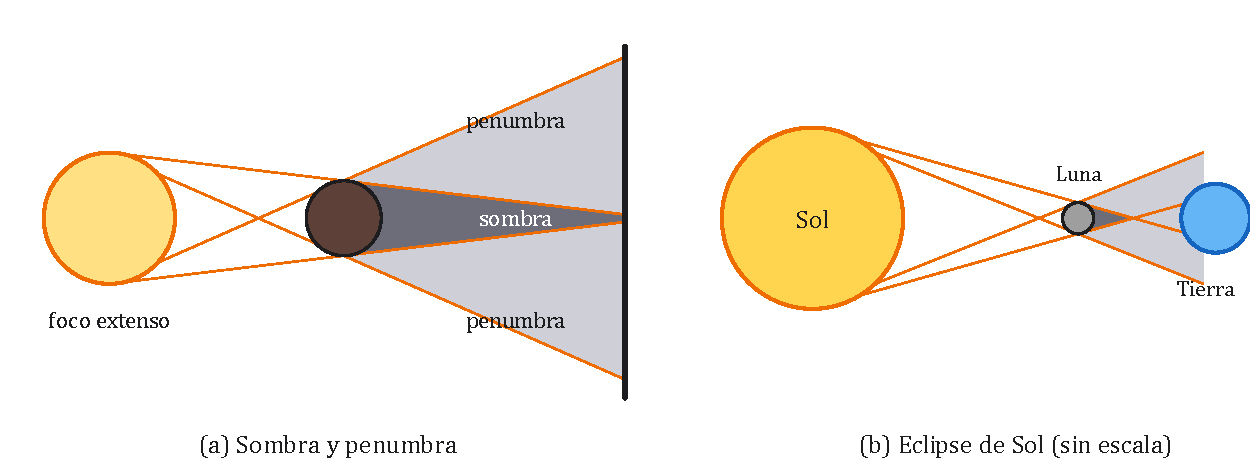
\includegraphics[width=0.95\linewidth]{images/UD3/sombras}
    \caption{(a) Sombra y penumbra de un cuerpo opaco. (b) En un eclipse de Sol la Luna proyecta su sombra sobre la Tierra.}
    \label{fig:opt-sombras}
\end{figure}

\subsection{Velocidad de la luz}\label{subsec:opt-velocidad}

Durante siglos se creyó que la luz se propagaba de forma instantánea. Galileo intentó medir su velocidad con faroles
entre dos colinas, sin éxito. En 1676 el danés Rømer la estimó por primera vez observando los eclipses de las lunas de
Júpiter y obtuvo unos \qty{2.1e8}{\m\per\second}. Fizeau (1849), con una rueda dentada, y Michelson, con espejos giratorios,
mejoraron mucho la medida. Hoy su valor en el vacío está fijado exactamente:
\begin{centeredequation}
    c = \qty{299792458}{\m\per\second} \approx \qty{3e8}{\m\per\second} \label{eq:opt-c}
\end{centeredequation}
En el aire es prácticamente la misma. En los demás medios transparentes la luz va más despacio: en el agua, a unos
\qty{2.25e8}{\m\per\second}, y en el vidrio, a unos \qty{2e8}{\m\per\second}.

\paragraph{El año luz.} En astronomía se usa como unidad de longitud el \azuln{año luz}: la distancia que recorre la luz en
el vacío en un año, \(\qty{1}{\text{a.l.}} = 3\cdot 10^8\cdot 365{,}25\cdot 86400 \approx \qty{9.46e15}{\m}\).

\begin{exercise}
    Cuando Marte está en conjunción, su distancia media al Sol es de unos \qty{2.28e8}{\km}. ¿Cuánto tarda en llegar a Marte
    la luz del Sol?
    \begin{solu}
        \(t = \dfrac{d}{c} = \dfrac{2{,}28\cdot 10^{11}}{3\cdot 10^8} = \textcolor{red}{\qty{760}{\second} \approx \qty{12.7}{\minute}}\).
    \end{solu}
\end{exercise}

\begin{exercise}
    Próxima Centauri, la estrella más cercana al Sol, está a \num{4.24} años luz. ¿A cuántos kilómetros está?
    \begin{solu}
        \(d = 4{,}24\cdot 9{,}46\cdot 10^{12}\ \unit{\km} = \textcolor{red}{\qty{4.01e13}{\km}}\).
    \end{solu}
\end{exercise}

\subsection{Índice de refracción}\label{subsec:opt-indice}

\begin{definition}[Índice de refracción]
    El \rojon{índice de refracción absoluto} de un medio es el cociente entre la velocidad de la luz en el vacío y su
    velocidad en ese medio:
    \begin{centeredequation}
        \boxed{n = \dfrac{c}{v}} \label{eq:opt-indice}
    \end{centeredequation}
    Es adimensional y siempre mayor que 1 (en el vacío, \(n = 1\); en el aire, \(n \approx 1\)).
\end{definition}

Un medio es \azuln{más refringente} que otro si su índice de refracción es mayor: en él la luz va más despacio. Para dos
medios, \(n_1 v_1 = n_2 v_2 = c\), y el \azuln{índice de refracción relativo} del medio 2 respecto del 1 es
\(n_{21} = \dfrac{n_2}{n_1} = \dfrac{v_1}{v_2}\).

\begin{table}[H]
    \centering
    \caption{Índices de refracción de algunas sustancias (luz amarilla)}
    \vspace{-5pt}
    \begin{tabular}{@{}lc@{\hspace{1.5cm}}lc@{}}
        \toprule
        \textbf{Sustancia} & \textbf{\(n\)} & \textbf{Sustancia} & \textbf{\(n\)} \\
        \midrule
        Aire & \num{1.0003} & Vidrio común & \num{1.52} \\[3pt]
        Agua & \num{1.33} & Vidrio \emph{flint} & \num{1.65} \\[3pt]
        Etanol & \num{1.36} & Cuarzo fundido & \num{1.46} \\[3pt]
        Hielo & \num{1.31} & Diamante & \num{2.42} \\
        \bottomrule
    \end{tabular}
    \label{tab:opt-indices}
\end{table}

\paragraph{Frecuencia y longitud de onda.} Al pasar de un medio a otro, la frecuencia de la luz no cambia (la impone el
foco), pero sí su velocidad y, por tanto, su longitud de onda: \(v_1 = \lambda_1\nu\) y \(v_2 = \lambda_2\nu\). Dividiendo:
\begin{centeredequation}
    \dfrac{\lambda_1}{\lambda_2} = \dfrac{v_1}{v_2} = \dfrac{n_2}{n_1} \qquad\Rightarrow\qquad \lambda = \dfrac{\lambda_0}{n} \label{eq:opt-lambda}
\end{centeredequation}
donde \(\lambda_0\) es la longitud de onda en el vacío. El color que percibimos depende de la frecuencia, así que un rayo
rojo sigue siendo rojo dentro del agua.

\begin{exercise}
    Un puntero láser de helio-neón emite luz roja de \qty{633}{\nm} en el vacío. ¿Cuál es su velocidad y su longitud de
    onda dentro del agua (\(n = 1{,}33\))?
    \begin{solu}
        \(v = \dfrac{c}{n} = \dfrac{3\cdot 10^8}{1{,}33} = \textcolor{red}{\qty{2.26e8}{\m\per\second}}\);
        \(\lambda = \dfrac{\lambda_0}{n} = \dfrac{633}{1{,}33} = \textcolor{red}{\qty{476}{\nm}}\).
        \textcolor{blue}{(Sigue viéndose roja: la frecuencia no cambia.)}
    \end{solu}
\end{exercise}

\begin{exercise}
    A veces se dice que «luz más luz puede dar oscuridad». ¿Tiene sentido?
    \begin{solu}
        \textcolor{red}{Sí: es una interferencia destructiva.} \textcolor{blue}{Si dos ondas luminosas coherentes llegan a un
        punto en oposición de fase (diferencia de caminos de un número impar de semilongitudes de onda), sus campos se
        anulan y en ese punto hay oscuridad. Es lo que se observa en las franjas oscuras del experimento de Young.}
    \end{solu}
\end{exercise}

\section{Reflexión y refracción de la luz}\label{sec:opt-reflexion-refraccion}

\subsection{Reflexión}\label{subsec:opt-reflexion}

Cuando la luz llega a la superficie de separación con otro medio, una parte vuelve al medio de donde venía: se refleja.
Si la superficie es lisa y pulida, todos los rayos de un haz paralelo se reflejan en la misma dirección
(\azuln{reflexión especular}); si es rugosa, cada rayo sale en una dirección distinta (\azuln{reflexión difusa},
figura~\ref{fig:opt-reflexion}). Gracias a la reflexión difusa vemos los objetos que no emiten luz propia desde cualquier
posición.

\begin{figure}[H]
    \centering
    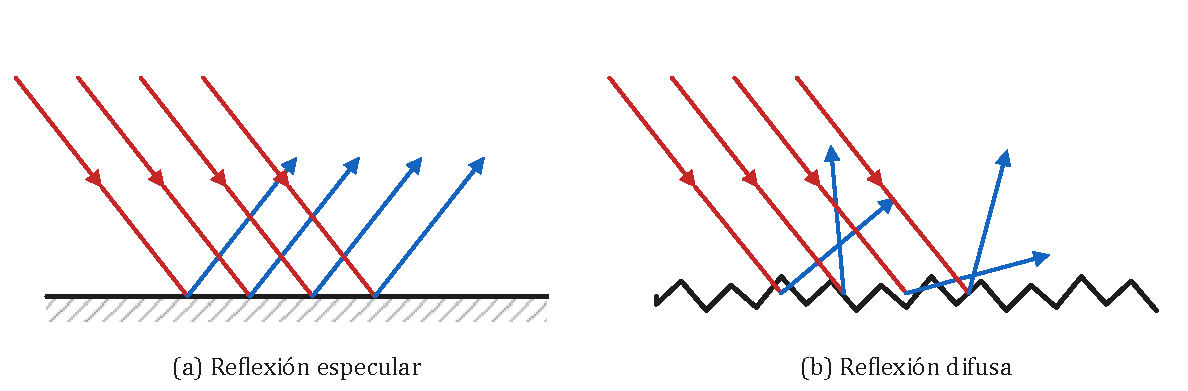
\includegraphics[width=0.85\linewidth]{images/UD3/reflexion_tipos}
    \caption{En una superficie pulida los rayos reflejados siguen paralelos; en una rugosa se dispersan.}
    \label{fig:opt-reflexion}
\end{figure}

Las \textbf{leyes de la reflexión}, que ya vimos para las ondas en la unidad anterior, son:
\begin{enumerate}[label=\numberballmDarkTeal]
    \item El rayo incidente, la normal y el rayo reflejado están en el mismo plano.
    \item El ángulo de incidencia es igual al de reflexión: \(\hat{\imath} = \hat r\).
\end{enumerate}

\subsection{Refracción. Ley de Snell}\label{subsec:opt-snell}

La \rojon{refracción} es el cambio de dirección de la luz al pasar de un medio a otro en el que tiene distinta velocidad.
Por ella un lápiz parece quebrado dentro de un vaso de agua o un pez parece estar más arriba de donde está. Las leyes son:
\begin{enumerate}[label=\numberballmDarkTeal]
    \item El rayo incidente, la normal y el rayo refractado están en el mismo plano.
    \item Se cumple la \rojon{ley de Snell}. Como \(v = c/n\):
    \begin{equation*}
        \dfrac{\sen\hat{\imath}}{\sen\hat r} = \dfrac{v_1}{v_2} = \dfrac{c/n_1}{c/n_2} = \dfrac{n_2}{n_1}
    \end{equation*}
    \begin{centeredequation}
        \boxed{n_1\sen\hat{\imath} = n_2\sen\hat r} \label{eq:opt-snell}
    \end{centeredequation}
\end{enumerate}

Si la luz pasa a un medio \textbf{más} refringente (\(n_2 > n_1\)), \(\sen\hat r < \sen\hat{\imath}\): el rayo se
\textbf{acerca} a la normal. Si pasa a uno \textbf{menos} refringente, se \textbf{aleja} de ella
(figura~\ref{fig:opt-refraccion}).

\begin{figure}[H]
    \centering
    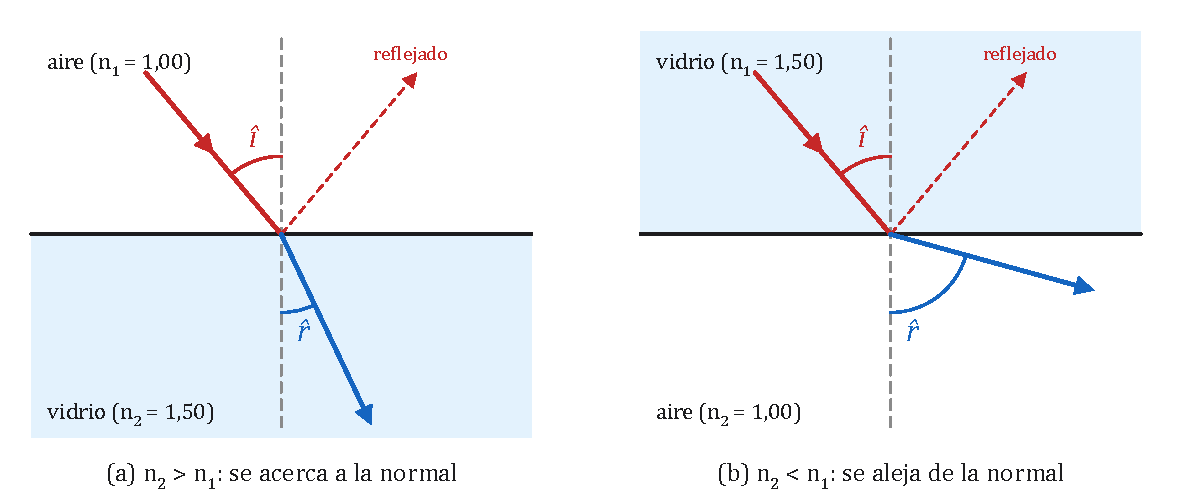
\includegraphics[width=0.92\linewidth]{images/UD3/refraccion_luz}
    \caption{Refracción entre aire y vidrio en los dos sentidos. En la superficie también se refleja parte de la luz.}
    \label{fig:opt-refraccion}
\end{figure}

\begin{exercise}
    Un rayo de luz pasa de un medio de índice \num{1.60} a otro de índice \num{1.40} con un ángulo de incidencia de \ang{35}.
    ¿Cuánto vale el ángulo de refracción? ¿Se acerca o se aleja de la normal?
    \begin{solu}
        \(\sen\hat r = \dfrac{n_1}{n_2}\sen\hat{\imath} = \dfrac{1{,}60}{1{,}40}\sen\ang{35} = 0{,}656 \Rightarrow \textcolor{red}{\hat r = \ang{41.0}}\):
        \textcolor{red}{se aleja de la normal}, \textcolor{blue}{porque pasa a un medio menos refringente.}
    \end{solu}
\end{exercise}

\begin{exercise}
    ¿Qué le ocurre a un rayo que llega perpendicularmente a la superficie de separación de dos medios?
    \begin{solu}
        \textcolor{blue}{Si \(\hat{\imath} = 0\), la ley de Snell da \(\sen\hat r = 0\):} \textcolor{red}{no se desvía},
        aunque \textcolor{red}{sí cambian su velocidad y su longitud de onda.}
    \end{solu}
\end{exercise}

\subsection{Ángulo límite y reflexión total}\label{subsec:opt-limite}

Cuando la luz pasa de un medio a otro \textbf{menos} refringente (\(n_1 > n_2\)), el ángulo de refracción es mayor que el
de incidencia. Si vamos aumentando \(\hat{\imath}\), llega un momento en que el rayo refractado sale rasante a la superficie
(\(\hat r = \ang{90}\)). Ese ángulo de incidencia es el \rojon{ángulo límite} \(\hat{\imath}_L\):
\begin{centeredequation}
    n_1\sen\hat{\imath}_L = n_2\sen\ang{90} \qquad\Rightarrow\qquad \boxed{\sen\hat{\imath}_L = \dfrac{n_2}{n_1}} \label{eq:opt-limite}
\end{centeredequation}
Para ángulos de incidencia mayores que el límite no hay rayo refractado: toda la luz se refleja. Es la \rojon{reflexión
total} (figura~\ref{fig:opt-limite}).

\begin{figure}[H]
    \centering
    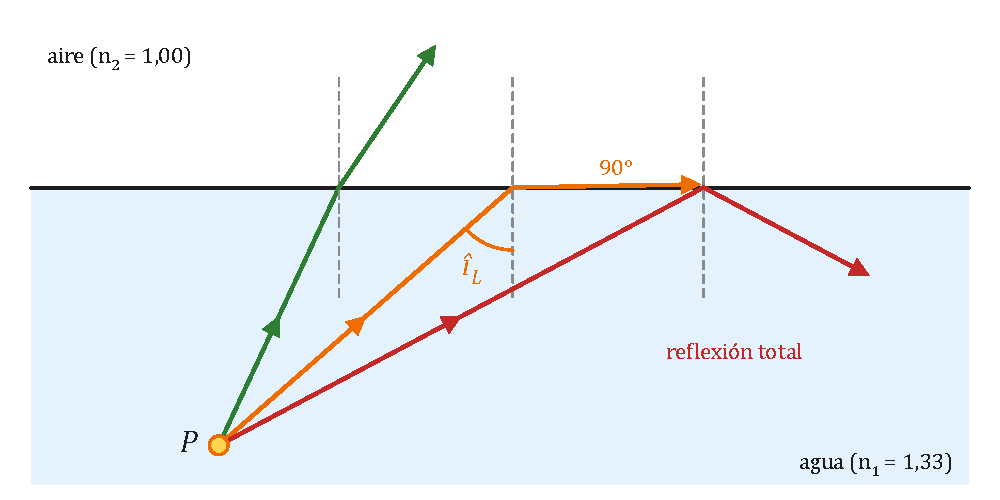
\includegraphics[width=0.62\linewidth]{images/UD3/angulo_limite}
    \caption{Rayos que salen de un punto sumergido. El rayo 2 incide con el ángulo límite y sale rasante; el 3, con un
    ángulo mayor, se refleja totalmente.}
    \label{fig:opt-limite}
\end{figure}

\begin{remark}
    La reflexión total solo es posible cuando la luz va hacia un medio \textbf{menos} refringente. Se aprovecha en la
    \textbf{fibra óptica}: la luz entra en un hilo de vidrio muy fino y avanza rebotando en sus paredes sin salir, aunque
    la fibra se curve. También en los prismas de los prismáticos y en el brillo de los diamantes, cuyo ángulo límite es muy
    pequeño (unos \ang{24}).
\end{remark}

\begin{exercise}
    ¿Cuál es el ángulo de incidencia mínimo para que la luz que va del agua (\(n = 1{,}33\)) al aire se refleje totalmente?
    \begin{solu}
        \(\sen\hat{\imath}_L = \dfrac{1}{1{,}33} = 0{,}752 \Rightarrow \textcolor{red}{\hat{\imath}_L = \ang{48.8}}\).
    \end{solu}
\end{exercise}

\begin{exercise}
    Un diamante (\(n = 2{,}42\)) sumergido en cierto líquido tiene un ángulo límite de \ang{34}. Calcula el índice de
    refracción del líquido y la velocidad de la luz en él.
    \begin{solu}
        \(n_{\text{liq}} = n_{\text{diam}}\sen\hat{\imath}_L = 2{,}42\sen\ang{34} = \textcolor{red}{1{,}35}\);
        \(v = \dfrac{c}{n} = \textcolor{red}{\qty{2.22e8}{\m\per\second}}\).
    \end{solu}
\end{exercise}

\begin{exercise}
    Una fibra óptica de cuarzo tiene un índice de refracción de \num{1.46}. ¿A qué velocidad viaja la luz por ella? ¿Cuál es
    el ángulo límite si la fibra está rodeada de aire?
    \begin{solu}
        \(v = \dfrac{3\cdot 10^8}{1{,}46} = \textcolor{red}{\qty{2.05e8}{\m\per\second}}\);
        \(\sen\hat{\imath}_L = \dfrac{1}{1{,}46} \Rightarrow \textcolor{red}{\hat{\imath}_L = \ang{43.2}}\).
    \end{solu}
\end{exercise}

\subsection{Lámina de caras planas y paralelas}\label{subsec:opt-lamina}

Una lámina transparente de caras paralelas (una ventana, un portaobjetos) refracta la luz dos veces
(figura~\ref{fig:opt-lamina}). Si a los dos lados hay el mismo medio:
\begin{equation*}
    n_1\sen\hat{\imath}_1 = n\sen\hat r_1 \quad\text{(primera cara)}, \qquad n\sen\hat r_1 = n_1\sen\hat{\imath}_2 \quad\text{(segunda cara)}
    \;\Rightarrow\; \hat{\imath}_1 = \hat{\imath}_2
\end{equation*}
\textbf{El rayo emergente es paralelo al incidente}, pero sale desplazado una distancia \(\delta\). Si \(e\) es el espesor de
la lámina, el camino recorrido dentro es \(AB = e/\cos\hat r_1\), y en el triángulo que forman \(AB\) y \(\delta\):
\begin{centeredequation}
    \boxed{\delta = AB\sen(\hat{\imath}_1 - \hat r_1) = e\,\dfrac{\sen(\hat{\imath}_1 - \hat r_1)}{\cos\hat r_1}} \label{eq:opt-lamina}
\end{centeredequation}

\begin{figure}[H]
    \centering
    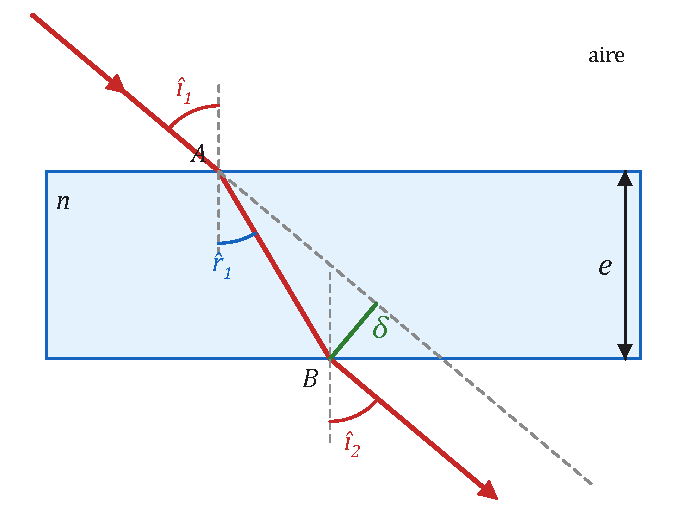
\includegraphics[width=0.48\linewidth]{images/UD3/lamina}
    \caption{Marcha de un rayo a través de una lámina de caras paralelas de espesor \(e\).}
    \label{fig:opt-lamina}
\end{figure}

\begin{exercise}
    Sobre una lámina de vidrio de \qty{2}{\cm} de espesor e índice \num{1.52}, situada en el aire, incide un rayo con un
    ángulo de \ang{40}. Calcula el ángulo de refracción dentro de la lámina, el ángulo de emergencia, el desplazamiento
    lateral y la distancia que recorre el rayo dentro del vidrio.
    \begin{solu}
        \(\sen\hat r_1 = \dfrac{\sen\ang{40}}{1{,}52} = 0{,}423 \Rightarrow \textcolor{red}{\hat r_1 = \ang{25.0}}\);
        \textcolor{red}{emerge con \ang{40}} \textcolor{blue}{(paralelo al incidente).}

        \(AB = \dfrac{2}{\cos\ang{25.0}} = \textcolor{red}{\qty{2.21}{\cm}}\);
        \(\delta = 2{,}21\sen(\ang{40} - \ang{25.0}) = \textcolor{red}{\qty{0.57}{\cm}}\).
    \end{solu}
\end{exercise}

\subsection{El prisma óptico}\label{subsec:opt-prisma}

Un \rojon{prisma óptico} es un medio transparente limitado por dos caras planas que forman un ángulo \(\varphi\), el
\azuln{ángulo del prisma}. Un rayo que entra por una cara se refracta dos veces y sale desviado hacia la base un ángulo
\(\delta\), el \azuln{ángulo de desviación} (figura~\ref{fig:opt-prisma}).

\begin{figure}[H]
    \centering
    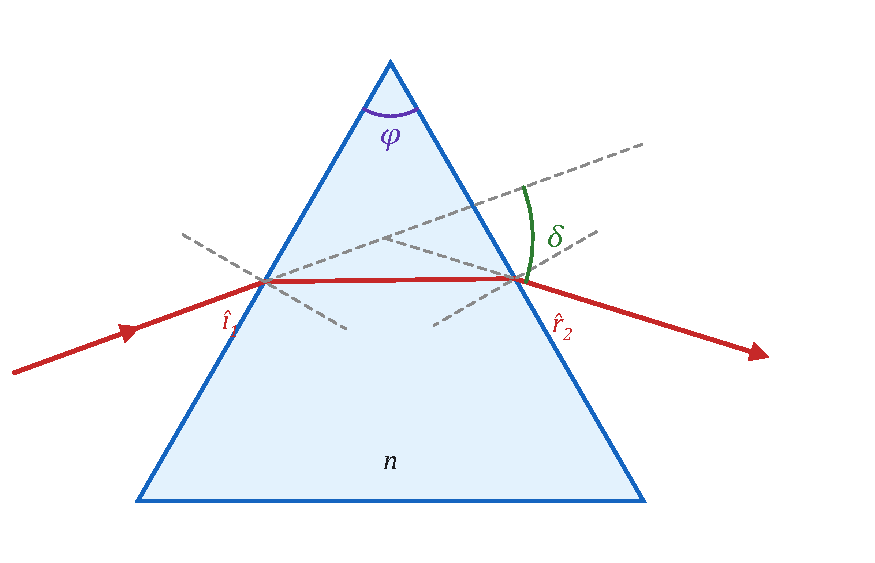
\includegraphics[width=0.55\linewidth]{images/UD3/prisma}
    \caption{Marcha de un rayo en un prisma de ángulo \(\varphi\). La desviación \(\delta\) es el ángulo entre la
    prolongación del rayo incidente y el rayo emergente.}
    \label{fig:opt-prisma}
\end{figure}

Si el prisma está en el aire, en cada cara se cumple la ley de Snell:
\begin{equation*}
    \sen\hat{\imath}_1 = n\sen\hat r_1 \qquad\qquad n\sen\hat{\imath}_2 = \sen\hat r_2
\end{equation*}
Las dos normales forman entre sí el mismo ángulo \(\varphi\) que las caras, y la geometría del triángulo que forman con el
rayo interior da:
\begin{centeredequation}
    \boxed{\varphi = \hat r_1 + \hat{\imath}_2} \qquad\qquad \boxed{\delta = \hat{\imath}_1 + \hat r_2 - \varphi} \label{eq:opt-prisma}
\end{centeredequation}

\paragraph{Desviación mínima.} La desviación depende del ángulo de incidencia y es \textbf{mínima} cuando el rayo atraviesa
el prisma simétricamente, paralelo a la base: entonces \(\hat{\imath}_1 = \hat r_2\) y \(\hat r_1 = \hat{\imath}_2 = \varphi/2\).
Con \(\delta_m = 2\hat{\imath}_1 - \varphi\):
\begin{centeredequation}
    \hat{\imath}_1 = \dfrac{\delta_m + \varphi}{2} \qquad\Rightarrow\qquad \boxed{n = \dfrac{\sen\dfrac{\delta_m + \varphi}{2}}{\sen\dfrac{\varphi}{2}}} \label{eq:opt-desviacion-minima}
\end{centeredequation}
Como \(\varphi\) y \(\delta_m\) se miden con facilidad, esta fórmula permite determinar en el laboratorio el índice de
refracción de un material tallado en forma de prisma.

\begin{exercise}
    Calcula la desviación mínima que produce un prisma equilátero (\(\varphi = \ang{60}\)) de vidrio de índice \num{1.5}.
    \begin{solu}
        \textcolor{blue}{En la desviación mínima \(\hat r_1 = \ang{30}\):} \(\sen\hat{\imath}_1 = 1{,}5\sen\ang{30} = 0{,}75 \Rightarrow \hat{\imath}_1 = \ang{48.6}\).
        \[ \delta_m = 2\hat{\imath}_1 - \varphi = 2\cdot\ang{48.6} - \ang{60} = \textcolor{red}{\ang{37.2}} \]
    \end{solu}
\end{exercise}

\subsection{Dispersión de la luz}\label{subsec:opt-dispersion}

La luz blanca es una mezcla de luces de distintas longitudes de onda (colores). En el vacío todas viajan a la misma
velocidad, pero en un medio material el índice de refracción depende ligeramente de la longitud de onda: es mayor para la
luz violeta (\(\lambda\) corta) que para la roja (\(\lambda\) larga). Por eso, al atravesar un prisma, cada color se desvía un
ángulo distinto y la luz blanca se separa en un abanico de colores, el \azuln{espectro visible}. Este fenómeno es la
\rojon{dispersión} de la luz (figura~\ref{fig:opt-dispersion}).

\begin{figure}[H]
    \centering
    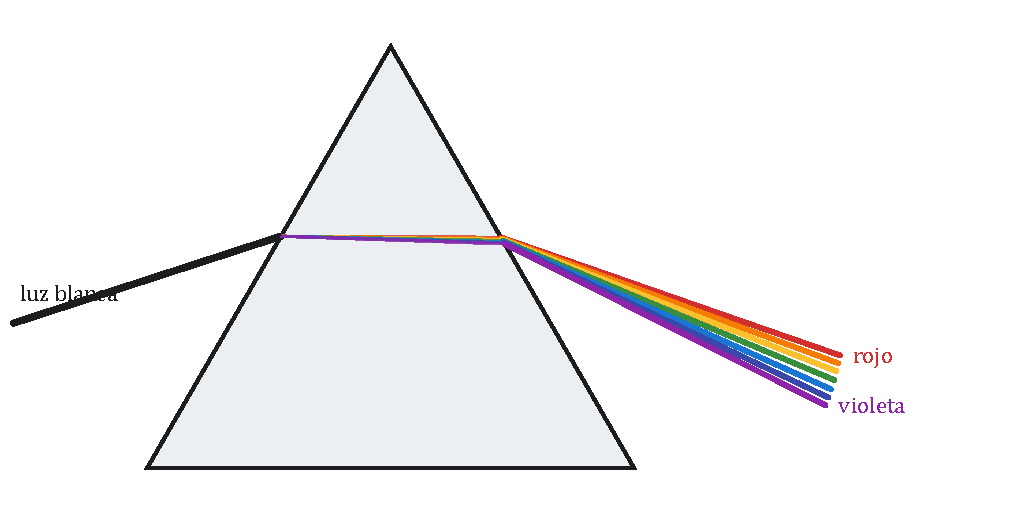
\includegraphics[width=0.66\linewidth]{images/UD3/dispersion}
    \caption{Dispersión de la luz blanca en un prisma: el violeta, con mayor índice de refracción, es el que más se desvía
    (la separación entre colores está exagerada).}
    \label{fig:opt-dispersion}
\end{figure}

El \textbf{arco iris} es un ejemplo natural: la luz del Sol se refracta al entrar en cada gota de lluvia, se refleja en su
parte posterior y vuelve a refractarse al salir, separándose en colores. Lo vemos cuando tenemos el Sol a la espalda y
llueve delante de nosotros, con el rojo en la parte exterior del arco y el violeta en la interior.

\section{Conceptos básicos de óptica geométrica}\label{sec:opt-conceptos}

La óptica geométrica estudia la formación de imágenes usando solo el concepto de rayo, sin tener en cuenta la naturaleza
ondulatoria de la luz. Se basa en cuatro hechos:
\begin{itemize}
    \item En un medio homogéneo e isótropo la luz se propaga en línea recta.
    \item Los rayos son independientes: si se cruzan, cada uno sigue su camino.
    \item Se cumplen las leyes de la reflexión y de la refracción.
    \item Los caminos son reversibles: si un rayo va de \(P\) a \(P'\), otro que salga de \(P'\) en sentido contrario
    llega a \(P\) por el mismo camino.
\end{itemize}

\paragraph{Definiciones.}
\begin{itemize}
    \item \textbf{Dioptrio}: superficie que separa dos medios transparentes de distinto índice de refracción. Puede ser
    plano o esférico.
    \item \textbf{Sistema óptico}: conjunto de dioptrios (y espejos). Su \azuln{eje óptico} o eje principal es la recta
    común que pasa por los centros de todas las superficies.
    \item En un dioptrio esférico, el \azuln{centro de curvatura} \(C\) es el centro de la esfera, \(R\) es su radio y el
    \azuln{vértice} \(O\) es el punto donde la superficie corta al eje.
    \item \textbf{Imagen real}: los rayos que salen de un punto objeto \(A\) se cortan, después de atravesar el sistema, en
    un punto \(A'\). Se puede recoger en una pantalla.
    \item \textbf{Imagen virtual}: los rayos salen divergentes y son sus \emph{prolongaciones} hacia atrás las que se cortan
    en \(A'\). No se puede recoger en una pantalla, pero el ojo la ve (como la imagen de un espejo plano).
\end{itemize}

\subsection{Convenio de signos}\label{subsec:opt-signos}

Usaremos el convenio de las normas \textbf{DIN}:
\begin{itemize}
    \item La luz llega siempre desde la \textbf{izquierda}.
    \item Las distancias horizontales se miden desde el vértice \(O\) (o el centro óptico): son \textbf{positivas hacia
    la derecha} y negativas hacia la izquierda. Por eso un objeto real situado delante del sistema tiene \(s < 0\).
    \item Las distancias verticales se miden desde el eje: positivas hacia arriba y negativas hacia abajo.
    \item Las magnitudes de la imagen se escriben con prima: \(s'\), \(y'\), \(f'\)\ldots
    \item El radio \(R\) es positivo si el centro de curvatura está a la derecha del vértice (superficie convexa vista
    desde la luz que llega) y negativo si está a la izquierda (cóncava).
\end{itemize}

\begin{remark}
    Los resultados de esta unidad valen para \textbf{rayos paraxiales}, los que forman ángulos pequeños con el eje (menos
    de unos \ang{10}). Para ellos \(\sen\alpha \approx \tg\alpha \approx \alpha\), y todos los rayos que salen de un punto
    se cortan en un único punto imagen.
\end{remark}

\section{El dioptrio esférico}\label{sec:opt-dioptrio}

Consideremos un dioptrio esférico de radio \(R\) que separa un medio de índice \(n\) (a la izquierda) de otro de índice
\(n'\). Un rayo sale de un punto \(A\) del eje, a una distancia \(s\) del vértice, se refracta en un punto \(P\) situado a
una altura \(h\) y corta al eje en \(A'\), a una distancia \(s'\) (figura~\ref{fig:opt-dioptrio}).

\begin{figure}[H]
    \centering
    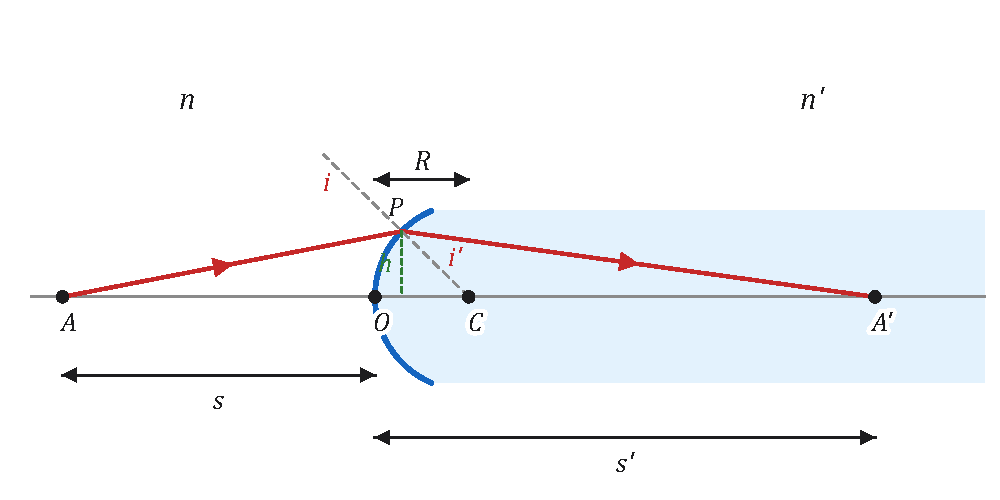
\includegraphics[width=0.66\linewidth]{images/UD3/dioptrio}
    \caption{Refracción en un dioptrio esférico convexo. La normal en \(P\) es la recta que pasa por el centro \(C\).}
    \label{fig:opt-dioptrio}
\end{figure}

Con rayos paraxiales, la ley de Snell queda \(n\,i = n'\,i'\). Los ángulos \(i\) e \(i'\) se pueden expresar con los
ángulos que forman con el eje el rayo incidente, el refractado y la normal, que para ángulos pequeños valen
aproximadamente \(h/s\), \(h/s'\) y \(h/R\). Sustituyendo y dividiendo por \(h\) se obtiene la \rojon{ecuación fundamental
del dioptrio esférico}:
\begin{centeredequation}
    \boxed{\dfrac{n'}{s'} - \dfrac{n}{s} = \dfrac{n' - n}{R}} \label{eq:opt-dioptrio}
\end{centeredequation}
No depende de \(h\): todos los rayos paraxiales que salen de \(A\) pasan por el mismo punto \(A'\).

\paragraph{Focos y distancias focales.}
\begin{itemize}
    \item El \azuln{foco imagen} \(F'\) es el punto donde convergen los rayos que llegan paralelos al eje (objeto en el
    infinito, \(s = -\infty\)). Su distancia al vértice es la \azuln{distancia focal imagen} \(f'\).
    \item El \azuln{foco objeto} \(F\) es el punto del eje del que tienen que salir los rayos para que, tras refractarse,
    salgan paralelos al eje (\(s' = \infty\)). Su distancia al vértice es la \azuln{distancia focal objeto} \(f\).
\end{itemize}
\begin{centeredequation}
    \dfrac{n'}{f'} - \dfrac{n}{-\infty} = \dfrac{n' - n}{R} \Rightarrow f' = R\,\dfrac{n'}{n' - n} \qquad\qquad
    \dfrac{n'}{\infty} - \dfrac{n}{f} = \dfrac{n' - n}{R} \Rightarrow f = -R\,\dfrac{n}{n' - n} \label{eq:opt-focales-dioptrio}
\end{centeredequation}
Se cumplen además \(\dfrac{f}{f'} = -\dfrac{n}{n'}\) y \(f + f' = R\). Dividiendo la ecuación fundamental entre \((n'-n)/R\)
se llega a la \azuln{ecuación de Gauss}: \(\dfrac{f'}{s'} + \dfrac{f}{s} = 1\).

\begin{figure}[H]
    \centering
    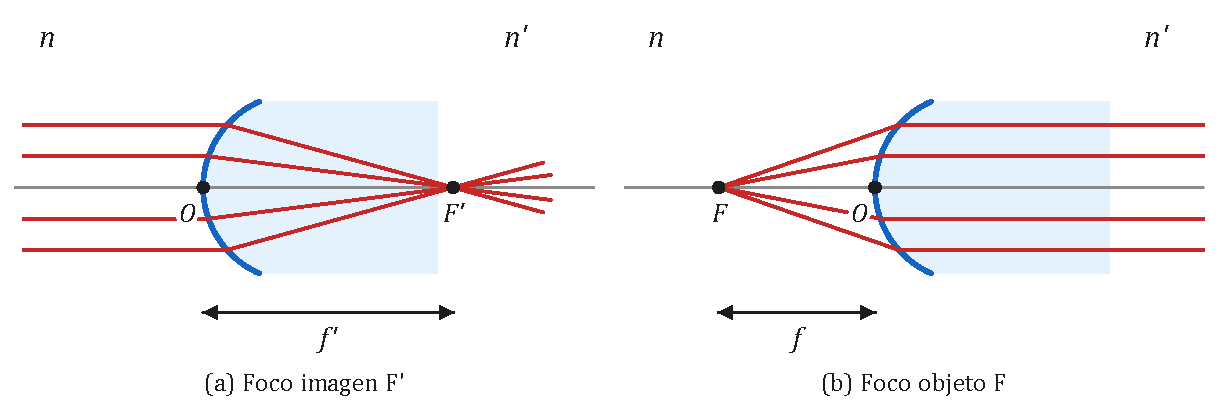
\includegraphics[width=0.9\linewidth]{images/UD3/dioptrio_focos}
    \caption{Focos de un dioptrio esférico convexo con \(n < n'\).}
    \label{fig:opt-dioptrio-focos}
\end{figure}

\paragraph{Construcción de imágenes.} Para hallar la imagen de un objeto \(AB\) perpendicular al eje se trazan desde \(B\)
dos de estos rayos y se busca su corte:
\begin{itemize}
    \item el rayo paralelo al eje, que se refracta pasando por \(F'\);
    \item el rayo que pasa por \(F\), que se refracta saliendo paralelo al eje;
    \item el rayo que pasa por \(C\), que no se desvía (llega perpendicular a la superficie).
\end{itemize}

\paragraph{Aumento lateral.} Es el cociente entre el tamaño de la imagen y el del objeto. Aplicando la ley de Snell al rayo
que llega al vértice:
\begin{centeredequation}
    \boxed{\beta = \dfrac{y'}{y} = \dfrac{n\,s'}{n'\,s}} \label{eq:opt-aumento-dioptrio}
\end{centeredequation}
Si \(\beta > 0\) la imagen es \textbf{derecha}; si \(\beta < 0\), \textbf{invertida}. Si \(|\beta| > 1\), es mayor que el objeto.

\begin{exercise}
    Un dioptrio esférico cóncavo de \qty{20}{\cm} de radio separa el aire (\(n = 1\)) de un vidrio de índice \num{1.5}. A
    \qty{40}{\cm} delante del vértice hay un objeto de \qty{3}{\cm} de altura. Calcula las distancias focales y la posición
    y el tamaño de la imagen.
    \begin{solu}
        \textcolor{blue}{Cóncavo: \(R = \qty{-20}{\cm}\); \(s = \qty{-40}{\cm}\).}

        \(f' = R\,\dfrac{n'}{n' - n} = -20\cdot\dfrac{1{,}5}{0{,}5} = \textcolor{red}{\qty{-60}{\cm}}\);
        \(f = -R\,\dfrac{n}{n' - n} = \textcolor{red}{\qty{40}{\cm}}\).

        \(\dfrac{1{,}5}{s'} = \dfrac{0{,}5}{-20} + \dfrac{1}{-40} = -0{,}05 \Rightarrow \textcolor{red}{s' = \qty{-30}{\cm}}\)
        \textcolor{blue}{(a la izquierda del vértice: imagen virtual).}

        \(\beta = \dfrac{1\cdot(-30)}{1{,}5\cdot(-40)} = 0{,}5 \Rightarrow \textcolor{red}{y' = \qty{1.5}{\cm}}\), \textcolor{red}{derecha y menor}.
    \end{solu}
\end{exercise}

\begin{exercise}
    Un dioptrio esférico convexo de \qty{30}{\cm} de radio separa dos medios de índices \num{1.2} y \num{1.8}. Calcula la
    posición y el tamaño de la imagen de un objeto de \qty{2}{\cm} situado \qty{90}{\cm} a la izquierda del vértice.
    \begin{solu}
        \(\dfrac{1{,}8}{s'} = \dfrac{1{,}8 - 1{,}2}{30} + \dfrac{1{,}2}{-90} = 0{,}02 - 0{,}0133 = 0{,}00667 \Rightarrow \textcolor{red}{s' = \qty{270}{\cm}}\)
        \textcolor{blue}{(imagen real).}

        \(\beta = \dfrac{1{,}2\cdot 270}{1{,}8\cdot(-90)} = -2 \Rightarrow \textcolor{red}{y' = \qty{-4}{\cm}}\): \textcolor{red}{invertida y el doble de grande}.
    \end{solu}
\end{exercise}

\subsection{El dioptrio plano}\label{subsec:opt-dioptrio-plano}

Un dioptrio plano es un dioptrio esférico de radio infinito. Con \(R = \infty\) la ecuación fundamental queda:
\begin{centeredequation}
    \dfrac{n'}{s'} = \dfrac{n}{s} \qquad\Rightarrow\qquad \boxed{\dfrac{s'}{s} = \dfrac{n'}{n}} \label{eq:opt-dioptrio-plano}
\end{centeredequation}
y el aumento es \(\beta = \dfrac{n s'}{n' s} = 1\): la imagen tiene el mismo tamaño que el objeto. Explica la
\textbf{profundidad aparente}: un objeto sumergido se ve más cerca de la superficie de lo que está, porque \(n' = 1 < n\) y
\(|s'| < |s|\) (figura~\ref{fig:opt-profundidad}).

\begin{figure}[H]
    \centering
    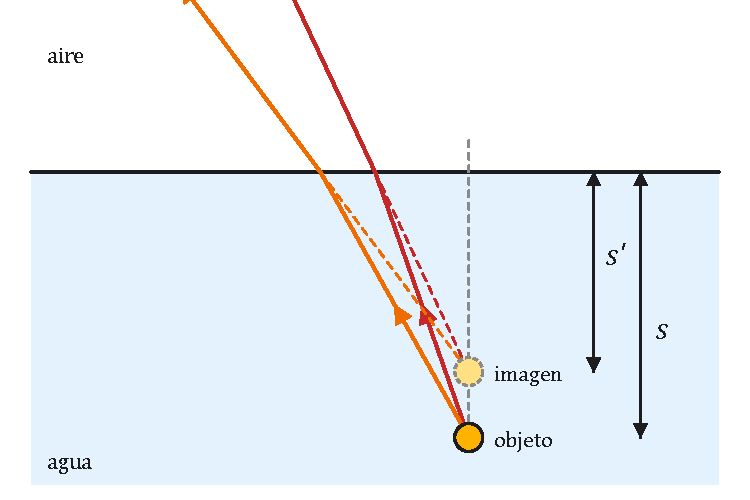
\includegraphics[width=0.5\linewidth]{images/UD3/profundidad}
    \caption{Los rayos que salen del objeto se alejan de la normal al salir al aire. Sus prolongaciones se cortan más arriba:
    el objeto parece estar a una profundidad \(s'\) menor que la real.}
    \label{fig:opt-profundidad}
\end{figure}

\begin{exercise}
    Un buceador mira hacia arriba desde el fondo de un embalse y ve un helicóptero que vuela a \qty{250}{\m} sobre el agua
    (\(n_{\text{agua}} = 1{,}33\)). ¿A qué altura le parece que está?
    \begin{solu}
        \textcolor{blue}{La luz va del aire (\(n = 1\)) al agua (\(n' = 1{,}33\)):}
        \(s' = s\,\dfrac{n'}{n} = 250\cdot 1{,}33 = \textcolor{red}{\qty{332.5}{\m}}\): \textcolor{blue}{lo ve más alto de lo que está.}
    \end{solu}
\end{exercise}

\begin{exercise}
    ¿A qué profundidad parece estar una moneda en el fondo de una piscina de \qty{2.2}{\m} llena de agua (\(n = 1{,}33\))?
    \begin{solu}
        \textcolor{blue}{Ahora la luz va del agua (\(n = 1{,}33\)) al aire (\(n' = 1\)):}
        \(s' = s\,\dfrac{n'}{n} = \dfrac{2{,}2}{1{,}33} = \textcolor{red}{\qty{1.65}{\m}}\).
    \end{solu}
\end{exercise}

\section{Espejos}\label{sec:opt-espejos}

Un espejo es una superficie que refleja casi toda la luz que le llega (normalmente, vidrio con una capa de plata o de
aluminio por detrás). La reflexión puede tratarse como una refracción especial: la luz sigue en el mismo medio, pero
cambia de sentido. Basta tomar \(n' = -n\) en las fórmulas del dioptrio.

\subsection{Espejo plano}\label{subsec:opt-espejo-plano}

Con \(n' = -n\) en la ecuación del dioptrio plano:
\begin{equation*}
    \dfrac{s'}{s} = \dfrac{-n}{n} = -1 \qquad\Rightarrow\qquad \boxed{s' = -s} \qquad\qquad \beta = 1
\end{equation*}
Un espejo plano da una imagen \textbf{virtual} (está detrás del espejo), \textbf{derecha}, del \textbf{mismo tamaño} y a la
\textbf{misma distancia} que el objeto (figura~\ref{fig:opt-espejo-plano}). Además, la imagen está invertida de izquierda a
derecha: la imagen de una mano derecha es una mano izquierda.

\begin{figure}[H]
    \centering
    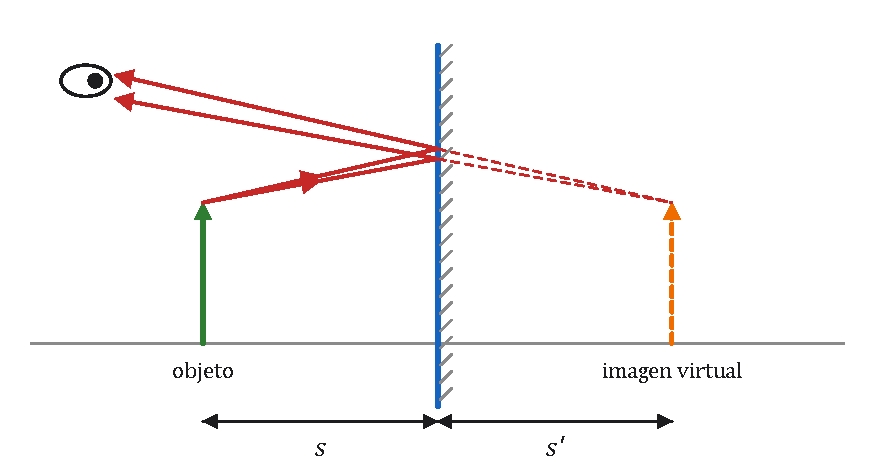
\includegraphics[width=0.56\linewidth]{images/UD3/espejo_plano}
    \caption{Los rayos reflejados que llegan al ojo parecen salir de un punto situado detrás del espejo.}
    \label{fig:opt-espejo-plano}
\end{figure}

\begin{exercise}
    ¿Qué altura mínima debe tener un espejo plano vertical para que una persona de \qty{1.70}{\m} se vea entera? ¿Depende
    de la distancia a la que se ponga?
    \begin{solu}
        \textcolor{blue}{Los rayos que van de la cabeza y de los pies a los ojos se reflejan en el espejo a mitad de camino
        entre cada punto y los ojos (la imagen está igual de lejos que la persona). Entre esos dos puntos de reflexión hay la
        mitad de la altura de la persona.}
        \textcolor{red}{El espejo debe medir \qty{0.85}{\m}} (la mitad de la altura), con su borde superior a media distancia
        entre los ojos y la coronilla. \textcolor{red}{No depende de la distancia al espejo.}
    \end{solu}
\end{exercise}

\subsection{Espejos esféricos}\label{subsec:opt-espejos-esfericos}

Un espejo esférico es un casquete de esfera que refleja la luz. Es \azuln{cóncavo} si la superficie reflectante es la
interior (su centro de curvatura está delante, a la izquierda: \(R < 0\)) y \azuln{convexo} si es la exterior (\(R > 0\)).

\paragraph{Foco y distancia focal.} Con \(n' = -n\) en las distancias focales del dioptrio:
\(f' = R\,\dfrac{-n}{-2n} = \dfrac{R}{2}\) y \(f = -R\,\dfrac{n}{-2n} = \dfrac{R}{2}\). En un espejo los dos focos coinciden en
un único punto \(F\), a mitad de camino entre el vértice y el centro de curvatura:
\begin{centeredequation}
    \boxed{f = f' = \dfrac{R}{2}} \label{eq:opt-focal-espejo}
\end{centeredequation}
En un espejo cóncavo los rayos que llegan paralelos al eje se reflejan pasando por \(F\) (\(f < 0\)); en uno convexo, son
sus prolongaciones las que pasan por \(F\), detrás del espejo (\(f > 0\), figura~\ref{fig:opt-espejos-foco}).

\begin{figure}[H]
    \centering
    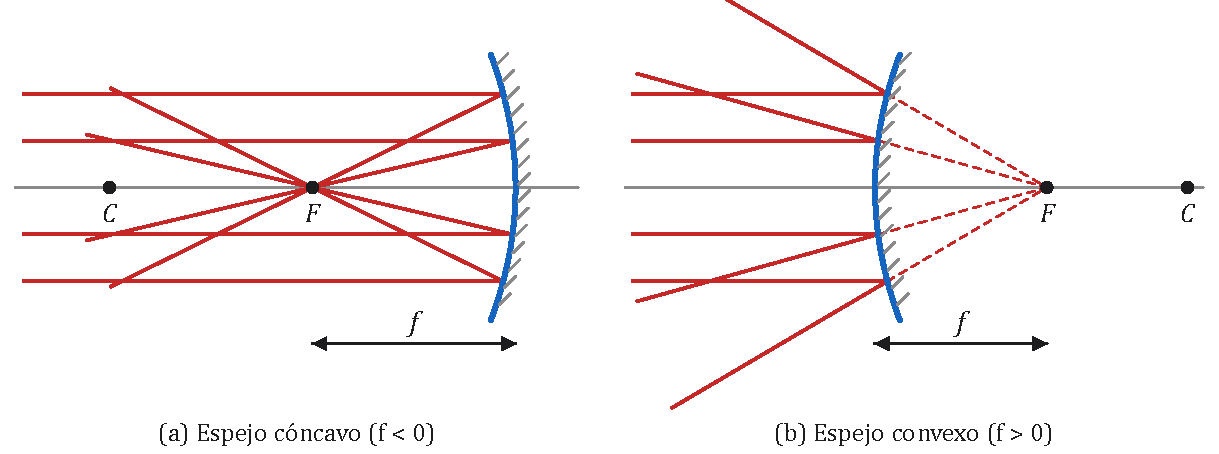
\includegraphics[width=0.9\linewidth]{images/UD3/espejos_foco}
    \caption{Foco de un espejo cóncavo (real) y de uno convexo (virtual).}
    \label{fig:opt-espejos-foco}
\end{figure}

\paragraph{Ecuación de los espejos y aumento.} Con \(n' = -n\) en la ecuación del dioptrio y dividiendo por \(-n\):
\begin{equation*}
    \dfrac{-n}{s'} - \dfrac{n}{s} = \dfrac{-2n}{R} \qquad\Rightarrow\qquad \dfrac{1}{s'} + \dfrac{1}{s} = \dfrac{2}{R}
\end{equation*}
\begin{centeredequation}
    \boxed{\dfrac{1}{s'} + \dfrac{1}{s} = \dfrac{1}{f}} \qquad\qquad \boxed{\beta = \dfrac{y'}{y} = -\dfrac{s'}{s}} \label{eq:opt-espejos}
\end{centeredequation}
Con el convenio de signos: si \(s' < 0\) la imagen está delante del espejo y es \textbf{real}; si \(s' > 0\), está detrás y
es \textbf{virtual}.

\paragraph{Construcción de imágenes.} Se usan dos de estos tres rayos que salen del extremo del objeto:
\begin{itemize}
    \item el que llega \textbf{paralelo al eje} se refleja pasando por \(F\) (en el convexo, su prolongación pasa por \(F\));
    \item el que pasa (o se dirige) \textbf{por el foco} se refleja paralelo al eje;
    \item el que pasa (o se dirige) \textbf{por el centro de curvatura} se refleja sobre sí mismo.
\end{itemize}

\begin{figure}[H]
    \centering
    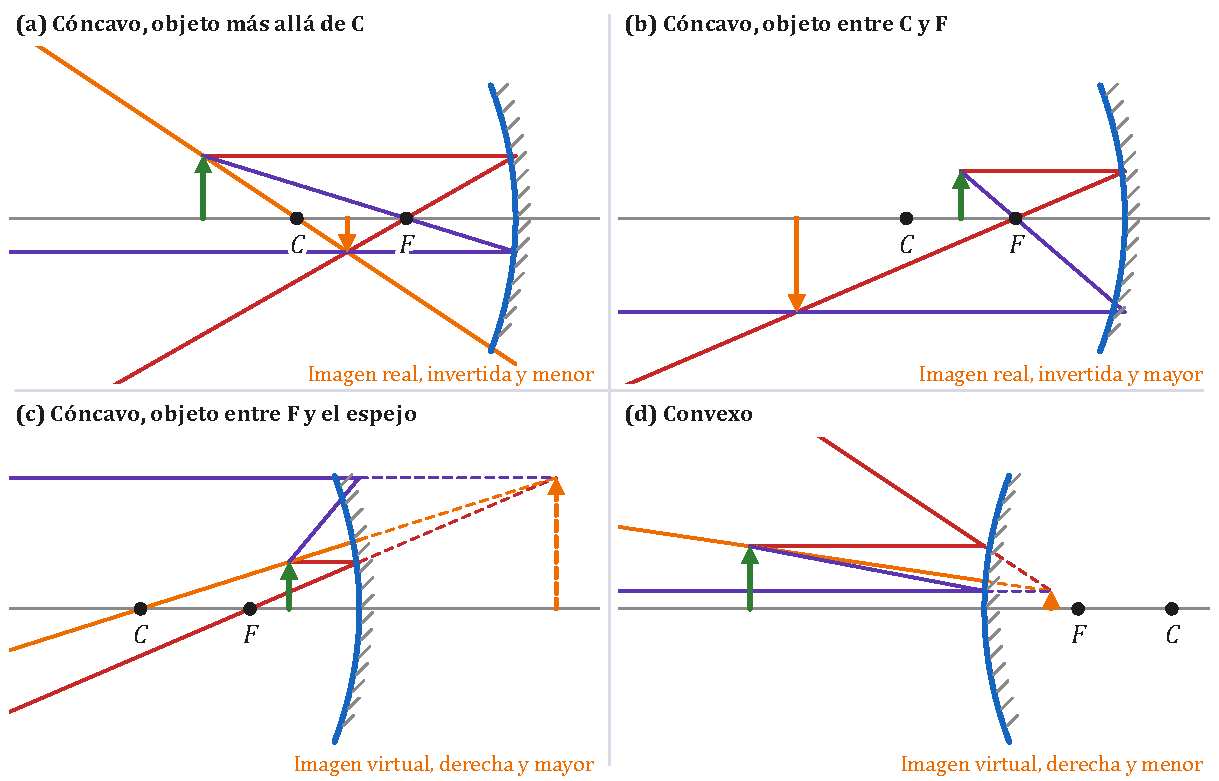
\includegraphics[width=\linewidth]{images/UD3/espejos_imagenes}
    \caption{Imágenes en espejos esféricos (objeto en verde, imagen en naranja; la imagen virtual, en discontinuo). Un espejo
    convexo siempre da una imagen virtual, derecha y menor, con un campo de visión amplio: por eso se usa en los
    retrovisores y en los cruces sin visibilidad.}
    \label{fig:opt-espejos-imagenes}
\end{figure}

\begin{table}[H]
    \centering
    \caption{Imagen que da un espejo cóncavo según la posición del objeto}
    \vspace{-5pt}
    \begin{tabular}{@{}lll@{}}
        \toprule
        \textbf{Posición del objeto} & \textbf{Posición de la imagen} & \textbf{Características} \\
        \midrule
        Más allá de \(C\) & Entre \(C\) y \(F\) & Real, invertida y menor \\[3pt]
        En \(C\) & En \(C\) & Real, invertida e igual \\[3pt]
        Entre \(C\) y \(F\) & Más allá de \(C\) & Real, invertida y mayor \\[3pt]
        En \(F\) & En el infinito & No se forma imagen \\[3pt]
        Entre \(F\) y el espejo & Detrás del espejo & Virtual, derecha y mayor \\
        \bottomrule
    \end{tabular}
    \label{tab:opt-espejo-concavo}
\end{table}

\begin{exercise}
    Construye la imagen de un objeto colocado en el centro de curvatura de un espejo cóncavo.
    \begin{solu}
        \textcolor{blue}{El rayo paralelo al eje se refleja por \(F\); el que pasa por \(F\) vuelve paralelo. Se cortan
        justo debajo de \(C\), a la misma distancia del eje que el extremo del objeto. Con la ecuación: \(s = R = 2f\),}
        \(\dfrac{1}{s'} = \dfrac{1}{f} - \dfrac{1}{2f} = \dfrac{1}{2f} \Rightarrow s' = 2f = R\), \(\beta = -1\).
        \textcolor{red}{La imagen está en \(C\) y es real, invertida y del mismo tamaño.}
    \end{solu}
\end{exercise}

\begin{exercise}
    Un objeto de \qty{1}{\cm} está a \qty{15}{\cm} a la izquierda de un espejo convexo de \qty{30}{\cm} de radio. Calcula
    la posición, el tamaño y las características de la imagen.
    \begin{solu}
        \textcolor{blue}{\(R = \qty{30}{\cm} \Rightarrow f = \qty{15}{\cm}\); \(s = \qty{-15}{\cm}\).}
        \(\dfrac{1}{s'} = \dfrac{1}{15} - \dfrac{1}{-15} = \dfrac{2}{15} \Rightarrow \textcolor{red}{s' = \qty{7.5}{\cm}}\);
        \(\beta = -\dfrac{7{,}5}{-15} = 0{,}5 \Rightarrow \textcolor{red}{y' = \qty{0.5}{\cm}}\).
        \textcolor{red}{Virtual (detrás del espejo), derecha y de la mitad de tamaño.}
    \end{solu}
\end{exercise}

\begin{exercise}
    Un objeto de \qty{2}{\cm} de altura está a \qty{75}{\cm} de un espejo cóncavo de \qty{50}{\cm} de radio. Calcula la
    distancia focal y la posición y el tamaño de la imagen.
    \begin{solu}
        \textcolor{blue}{\(R = \qty{-50}{\cm}\):} \(f = \dfrac{R}{2} = \textcolor{red}{\qty{-25}{\cm}}\).
        \(\dfrac{1}{s'} = \dfrac{1}{-25} - \dfrac{1}{-75} = -\dfrac{2}{75} \Rightarrow \textcolor{red}{s' = \qty{-37.5}{\cm}}\).

        \(\beta = -\dfrac{-37{,}5}{-75} = -0{,}5 \Rightarrow \textcolor{red}{y' = \qty{-1}{\cm}}\): \textcolor{red}{real, invertida y menor}.
    \end{solu}
\end{exercise}

\begin{exercise}
    Resuelve la actividad anterior si el espejo es convexo.
    \begin{solu}
        \textcolor{blue}{\(R = \qty{50}{\cm}\):} \(f = \textcolor{red}{\qty{25}{\cm}}\).
        \(\dfrac{1}{s'} = \dfrac{1}{25} + \dfrac{1}{75} = \dfrac{4}{75} \Rightarrow \textcolor{red}{s' = \qty{18.75}{\cm}}\);
        \(\beta = 0{,}25 \Rightarrow \textcolor{red}{y' = \qty{0.5}{\cm}}\): \textcolor{red}{virtual, derecha y menor}.
    \end{solu}
\end{exercise}

\section{Lentes delgadas}\label{sec:opt-lentes}

Una \rojon{lente} es un medio transparente limitado por dos superficies, al menos una de ellas esférica: es un sistema de
dos dioptrios. Si su espesor es pequeño comparado con los radios de curvatura, es una \azuln{lente delgada}, y se puede
considerar que los dos vértices coinciden en un único punto, el \azuln{centro óptico} \(O\).
\begin{itemize}
    \item Las \textbf{lentes convergentes} son más gruesas en el centro que en los bordes: biconvexas, planoconvexas y
    meniscos convergentes. Los rayos paralelos al eje convergen en el foco imagen.
    \item Las \textbf{lentes divergentes} son más gruesas en los bordes: bicóncavas, planocóncavas y meniscos divergentes.
    Los rayos paralelos salen separándose, como si vinieran del foco imagen.
\end{itemize}

\begin{figure}[H]
    \centering
    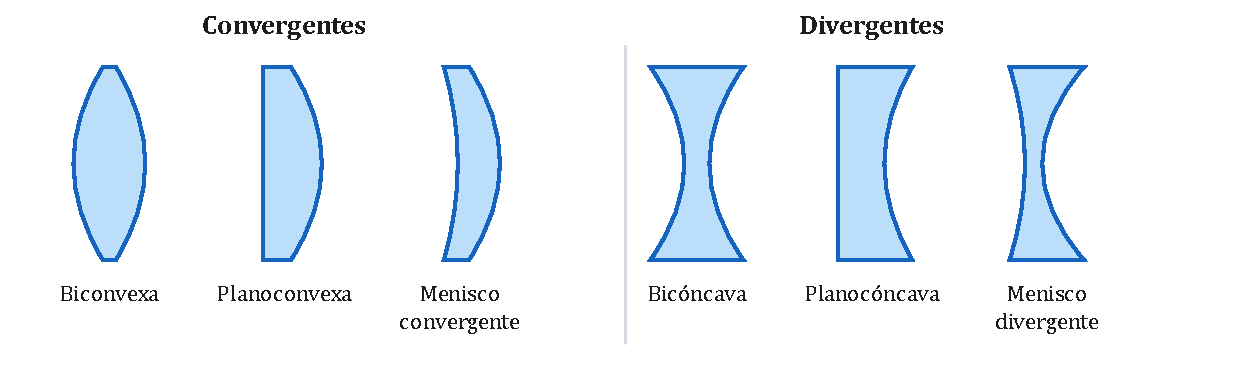
\includegraphics[width=0.9\linewidth]{images/UD3/lentes_tipos}
    \caption{Tipos de lentes. En los esquemas, una lente delgada se representa con un segmento con puntas de flecha
    (convergente) o con las puntas hacia dentro (divergente).}
    \label{fig:opt-lentes-tipos}
\end{figure}

\paragraph{Ecuación del constructor de lentes.} Aplicando la ecuación del dioptrio a las dos caras de una lente de índice
\(n\) en el aire (la imagen de la primera cara hace de objeto para la segunda) y sumando se obtiene:
\begin{centeredequation}
    \dfrac{1}{s'} - \dfrac{1}{s} = (n - 1)\left(\dfrac{1}{R_1} - \dfrac{1}{R_2}\right) \label{eq:opt-constructor}
\end{centeredequation}
Si el objeto está en el infinito, la imagen se forma en el foco imagen, \(s' = f'\):
\begin{centeredequation}
    \dfrac{1}{f'} = (n - 1)\left(\dfrac{1}{R_1} - \dfrac{1}{R_2}\right) \label{eq:opt-focal-lente}
\end{centeredequation}

\paragraph{Ecuación de las lentes delgadas y aumento.} Comparando las dos ecuaciones anteriores:
\begin{centeredequation}
    \boxed{\dfrac{1}{s'} - \dfrac{1}{s} = \dfrac{1}{f'}} \qquad\qquad \boxed{\beta = \dfrac{y'}{y} = \dfrac{s'}{s}} \label{eq:opt-lentes}
\end{centeredequation}
En una lente los dos focos están a ambos lados, a la misma distancia: \(f = -f'\). En una lente convergente \(f' > 0\) (el
foco imagen está a la derecha) y en una divergente \(f' < 0\) (figura~\ref{fig:opt-lentes-focos}). En las lentes, a
diferencia de los espejos, la imagen es \textbf{real} si \(s' > 0\) (se forma detrás de la lente) y \textbf{virtual} si
\(s' < 0\).

\begin{figure}[H]
    \centering
    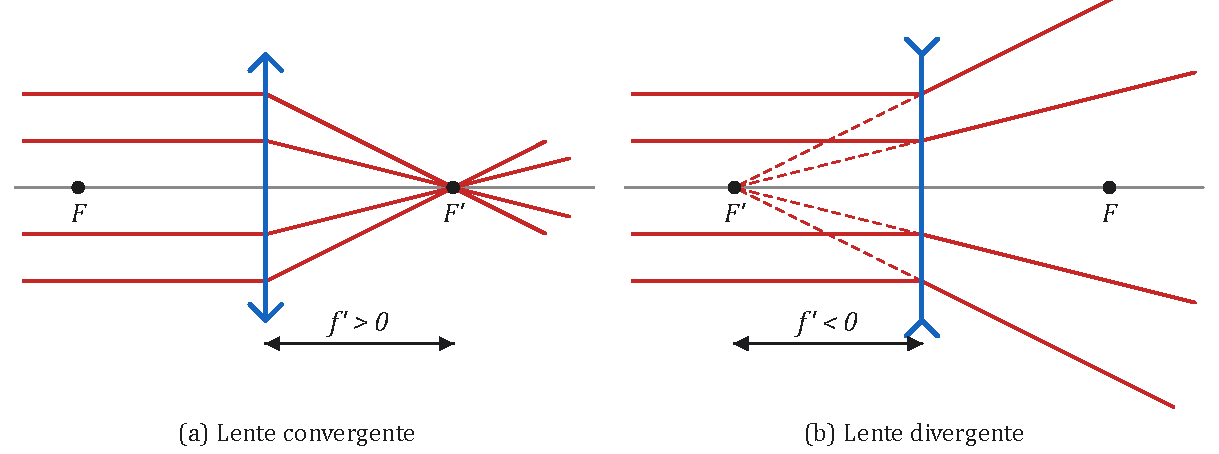
\includegraphics[width=0.9\linewidth]{images/UD3/lentes_focos}
    \caption{Foco imagen \(F'\) de una lente convergente (real) y de una divergente (virtual).}
    \label{fig:opt-lentes-focos}
\end{figure}

\paragraph{Potencia de una lente.} Es la inversa de la distancia focal imagen. Si \(f'\) se mide en metros, la potencia se
mide en \azuln{dioptrías} (\unit{D}, \(\qty{1}{D} = \qty{1}{\per\m}\)):
\begin{centeredequation}
    \boxed{P = \dfrac{1}{f'}} \label{eq:opt-potencia}
\end{centeredequation}
Las lentes convergentes tienen potencia positiva y las divergentes, negativa. Si se ponen varias lentes delgadas juntas, la
potencia del conjunto es la suma: \(P = P_1 + P_2 + \cdots\)

\paragraph{Construcción de imágenes.} Se usan dos de estos tres rayos:
\begin{itemize}
    \item el que llega \textbf{paralelo al eje} sale pasando por \(F'\) (en la divergente, su prolongación pasa por \(F'\));
    \item el que pasa (o se dirige) \textbf{por \(F\)} sale paralelo al eje;
    \item el que pasa por el \textbf{centro óptico} no se desvía.
\end{itemize}

\begin{figure}[H]
    \centering
    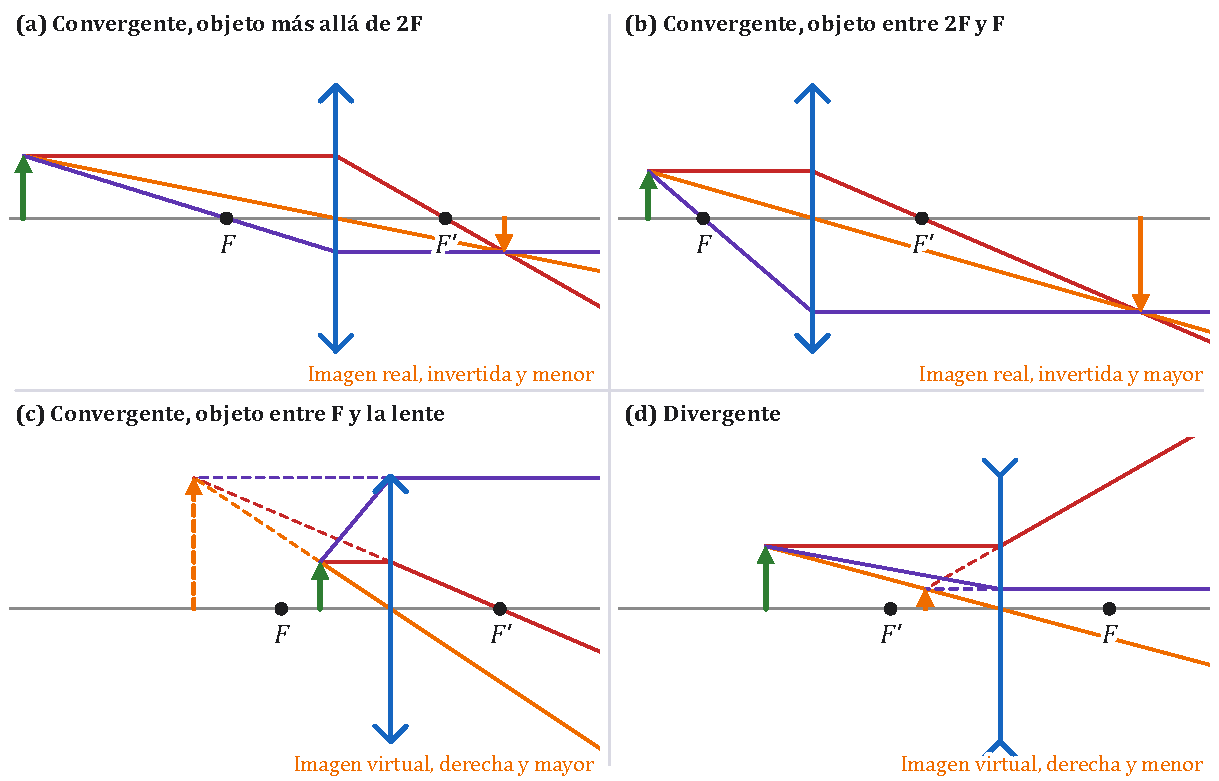
\includegraphics[width=\linewidth]{images/UD3/lentes_imagenes}
    \caption{Imágenes en lentes delgadas. Una lente divergente da siempre una imagen virtual, derecha y menor.}
    \label{fig:opt-lentes-imagenes}
\end{figure}

\begin{exercise}
    Una lente biconvexa de vidrio (\(n = 1{,}5\)) tiene dos caras de \qty{20}{\cm} de radio. Calcula su distancia focal y su
    potencia.
    \begin{solu}
        \textcolor{blue}{Primera cara convexa, \(R_1 = \qty{20}{\cm}\); segunda cóncava vista desde la luz, \(R_2 = \qty{-20}{\cm}\).}
        \[ \dfrac{1}{f'} = 0{,}5\left(\dfrac{1}{20} + \dfrac{1}{20}\right) = 0{,}05\ \unit{\per\cm} \;\Rightarrow\; \textcolor{red}{f' = \qty{20}{\cm}} \]
        \(P = \dfrac{1}{0{,}20} = \textcolor{red}{\qty{5}{D}}\).
    \end{solu}
\end{exercise}

\begin{exercise}
    Un objeto de \qty{3}{\cm} de altura está a \qty{25}{\cm} de una lente convergente de \qty{15}{\cm} de distancia focal.
    Calcula la posición y el tamaño de la imagen.
    \begin{solu}
        \(\dfrac{1}{s'} = \dfrac{1}{15} + \dfrac{1}{-25} = \dfrac{2}{75} \Rightarrow \textcolor{red}{s' = \qty{37.5}{\cm}}\) \textcolor{blue}{(real, detrás de la lente)};
        \(\beta = \dfrac{37{,}5}{-25} = -1{,}5 \Rightarrow \textcolor{red}{y' = \qty{-4.5}{\cm}}\): \textcolor{red}{invertida y mayor}.
    \end{solu}
\end{exercise}

\section{El ojo humano}\label{sec:opt-ojo}

El ojo es un sistema óptico casi esférico (figura~\ref{fig:opt-ojo}):
\begin{itemize}
    \item La \textbf{córnea} es la parte delantera, transparente, de la membrana exterior (esclerótica). Es la superficie
    que más desvía la luz.
    \item El \textbf{iris} es el diafragma de color; regula la cantidad de luz que entra cambiando el diámetro de la
    \textbf{pupila}.
    \item El \textbf{cristalino} es una lente convergente flexible. Delante tiene el \emph{humor acuoso} y detrás el
    \emph{humor vítreo}, con índices parecidos al del agua.
    \item La \textbf{retina} recubre el fondo del ojo. Sus células (conos y bastones) transforman la luz en señales
    eléctricas que el \textbf{nervio óptico} lleva al cerebro.
\end{itemize}
El sistema córnea-cristalino forma en la retina una imagen \textbf{real, invertida y menor}; el cerebro se encarga de
«darle la vuelta».

\begin{figure}[H]
    \centering
    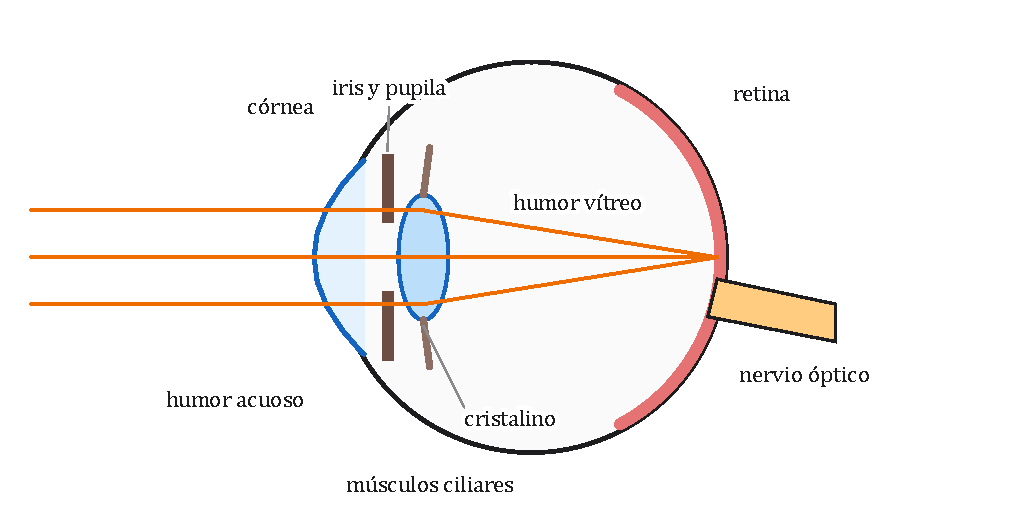
\includegraphics[width=0.66\linewidth]{images/UD3/ojo}
    \caption{Partes del ojo humano. La luz de un objeto lejano converge sobre la retina.}
    \label{fig:opt-ojo}
\end{figure}

\paragraph{Acomodación.} La distancia entre el cristalino y la retina es fija, así que para enfocar objetos a distintas
distancias el ojo cambia la curvatura del cristalino con los \emph{músculos ciliares}: es la \azuln{acomodación}. El punto
más lejano que se ve nítido sin esfuerzo es el \azuln{punto remoto} (el infinito para un ojo normal), y el más cercano, el
\azuln{punto próximo} (unos \qty{25}{\cm} en un adulto joven; unos \qty{7}{\cm} en un niño y hasta \qty{2}{\m} en una persona
mayor).

\subsection{Defectos de la visión}\label{subsec:opt-defectos}

\begin{itemize}
    \item \textbf{Miopía}. El ojo es demasiado convergente (o demasiado largo): la imagen de los objetos lejanos se forma
    \emph{delante} de la retina y se ven borrosos. Se corrige con \textbf{lentes divergentes}, cuyo foco imagen coincide con
    el punto remoto del ojo, o con cirugía láser de la córnea.
    \item \textbf{Hipermetropía}. El ojo es poco convergente: la imagen de los objetos cercanos se formaría \emph{detrás} de
    la retina. El punto próximo está más lejos de lo normal. Se corrige con \textbf{lentes convergentes}.
    \item \textbf{Presbicia} o vista cansada. Con la edad el cristalino pierde flexibilidad, la acomodación disminuye y el
    punto próximo se aleja. Se corrige con lentes convergentes para ver de cerca.
    \item \textbf{Astigmatismo}. La córnea no es perfectamente esférica y el ojo no enfoca a la vez las líneas verticales y
    las horizontales. Se corrige con lentes cilíndricas.
\end{itemize}

\begin{figure}[H]
    \centering
    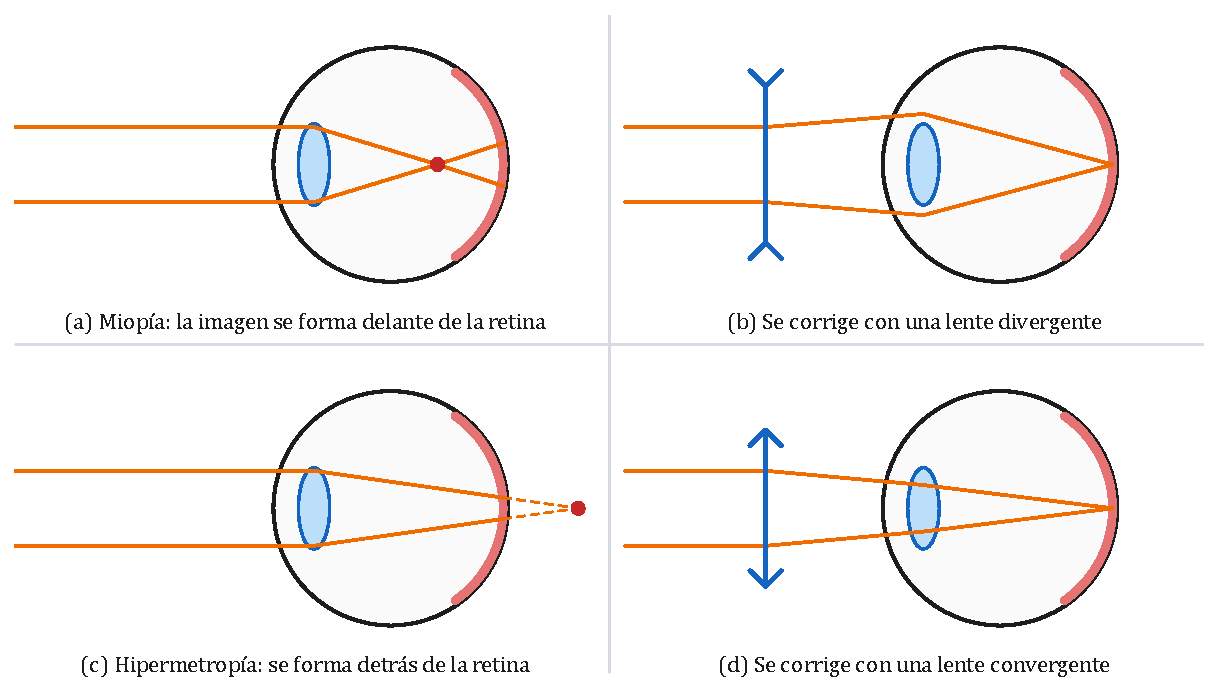
\includegraphics[width=0.9\linewidth]{images/UD3/defectos_vision}
    \caption{Miopía e hipermetropía y su corrección.}
    \label{fig:opt-defectos}
\end{figure}

\begin{exercise}
    El punto remoto de una persona miope está a \qty{50}{\cm}. ¿Qué lente necesita para ver bien de lejos?
    \begin{solu}
        \textcolor{blue}{La lente debe formar la imagen de un objeto en el infinito en el punto remoto: \(s = -\infty\), \(s' = \qty{-50}{\cm}\).}
        \(\dfrac{1}{f'} = \dfrac{1}{-50} - 0 \Rightarrow f' = \qty{-50}{\cm}\):
        \textcolor{red}{divergente de \(P = \dfrac{1}{-0{,}5} = \qty{-2}{D}\)}.
    \end{solu}
\end{exercise}

\begin{exercise}
    Una persona hipermétrope tiene el punto próximo a \qty{75}{\cm}. ¿Qué lente necesita para leer a \qty{25}{\cm}?
    \begin{solu}
        \textcolor{blue}{La lente debe dar, de un texto a \(s = \qty{-25}{\cm}\), una imagen virtual en su punto próximo, \(s' = \qty{-75}{\cm}\):}
        \(\dfrac{1}{f'} = \dfrac{1}{-75} - \dfrac{1}{-25} = \dfrac{2}{75} \Rightarrow f' = \qty{37.5}{\cm}\):
        \textcolor{red}{convergente de \(P = \qty{2.67}{D}\)}.
    \end{solu}
\end{exercise}

\section{Instrumentos ópticos}\label{sec:opt-instrumentos}

\subsection{La lupa}\label{subsec:opt-lupa}

Para ver un objeto con detalle lo acercamos al ojo: así ocupa un ángulo mayor y su imagen en la retina es más grande. Pero
no podemos acercarlo más que el punto próximo. La \rojon{lupa} es una lente convergente de distancia focal corta: si se pone
el objeto \textbf{entre el foco y la lente}, da una imagen \textbf{virtual, derecha y mayor} (figura~\ref{fig:opt-lupa}). Si
el objeto se coloca justo en el foco, la imagen está en el infinito y se ve sin necesidad de acomodar. El aumento de una
lupa en ese caso es aproximadamente \(M = \dfrac{\qty{0.25}{\m}}{f'}\).

\begin{figure}[H]
    \centering
    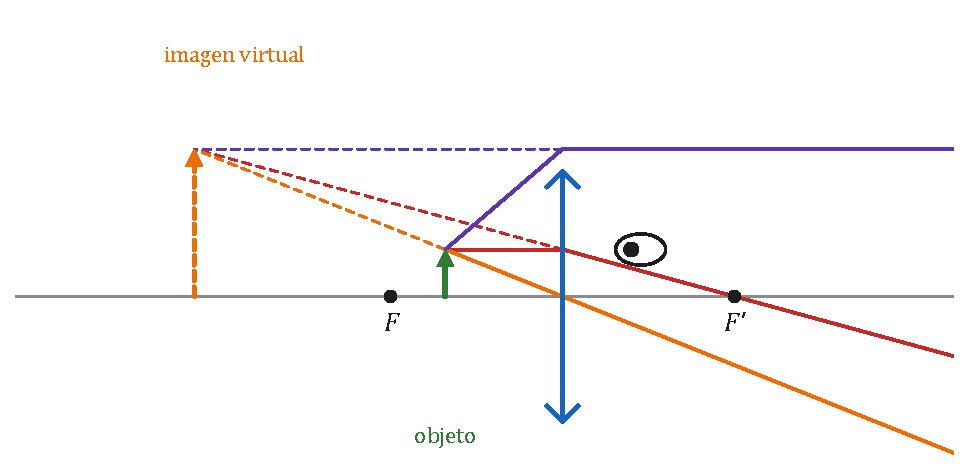
\includegraphics[width=0.62\linewidth]{images/UD3/lupa}
    \caption{Con el objeto dentro de la distancia focal, la lupa da una imagen virtual y aumentada.}
    \label{fig:opt-lupa}
\end{figure}

\begin{exercise}
    Queremos observar un mosquito con una lupa de \qty{4}{\cm} de distancia focal y ver su imagen 15 veces mayor. ¿A qué
    distancia de la lupa hay que ponerlo?
    \begin{solu}
        \textcolor{blue}{Imagen derecha: \(\beta = \dfrac{s'}{s} = 15 \Rightarrow s' = 15s\). En la ecuación de las lentes:}
        \[ \dfrac{1}{15s} - \dfrac{1}{s} = \dfrac{1}{4} \;\Rightarrow\; \dfrac{-14}{15s} = \dfrac{1}{4} \;\Rightarrow\; \textcolor{red}{s = \qty{-3.73}{\cm}} \]
        \textcolor{blue}{A \qty{3.73}{\cm} de la lupa, dentro de la distancia focal; la imagen está en \(s' = \qty{-56}{\cm}\).}
    \end{solu}
\end{exercise}

\subsection{El microscopio}\label{subsec:opt-microscopio}

El \rojon{microscopio} tiene dos lentes convergentes de distancia focal pequeña (figura~\ref{fig:opt-microscopio}):
\begin{itemize}
    \item El \textbf{objetivo}, la lente cercana al objeto. El objeto se coloca un poco más allá de su foco y el objetivo
    da una imagen \(y'_1\) \textbf{real, invertida y mucho mayor}.
    \item El \textbf{ocular}, la lente por la que se mira. La imagen \(y'_1\) queda entre el ocular y su foco objeto, y el
    ocular actúa como una lupa: da una imagen final \(y'_2\) \textbf{virtual} y mucho mayor (invertida respecto del objeto).
\end{itemize}
El aumento total es el producto de los aumentos del objetivo y del ocular: un objetivo \(40\times\) con un ocular
\(10\times\) aumenta \(400\) veces.

\begin{figure}[H]
    \centering
    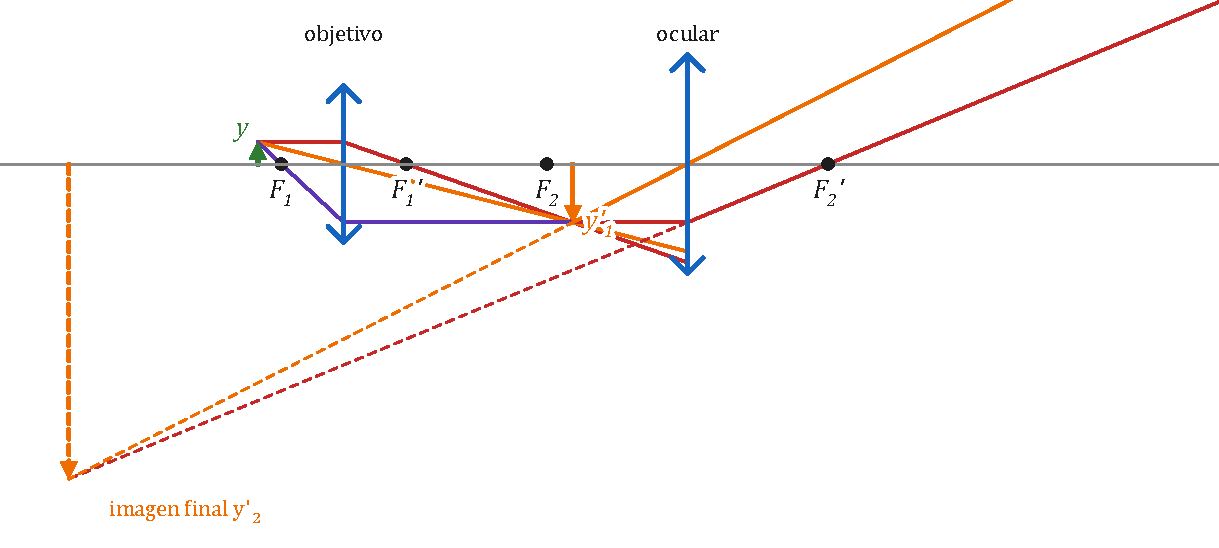
\includegraphics[width=0.9\linewidth]{images/UD3/microscopio}
    \caption{Formación de la imagen en un microscopio.}
    \label{fig:opt-microscopio}
\end{figure}

\section{Resumen de fórmulas}\label{sec:opt-resumen}

\begin{table}[H]
    \centering
    \caption{Fórmulas principales de la óptica geométrica (convenio DIN)}
    \vspace{-5pt}
    \begin{tabular}{@{}lL{10cm}@{}}
        \toprule
        \textbf{Magnitud} & \textbf{Expresión} \\
        \midrule
        Índice de refracción & \(n = c/v\), \quad \(\lambda = \lambda_0/n\) \\[3pt]
        Ley de Snell & \(n_1\sen\hat{\imath} = n_2\sen\hat r\) \\[3pt]
        Ángulo límite & \(\sen\hat{\imath}_L = n_2/n_1\) \quad (\(n_1 > n_2\)) \\[3pt]
        Lámina de caras paralelas & \(\delta = e\sen(\hat{\imath} - \hat r)/\cos\hat r\) \\[3pt]
        Prisma & \(\varphi = \hat r_1 + \hat{\imath}_2\), \quad \(\delta = \hat{\imath}_1 + \hat r_2 - \varphi\) \\[3pt]
        Desviación mínima & \(n = \sen\frac{\delta_m + \varphi}{2}\big/\sen\frac{\varphi}{2}\) \\[3pt]
        Dioptrio esférico & \(n'/s' - n/s = (n' - n)/R\), \quad \(\beta = n s'/(n' s)\) \\[3pt]
        Focales del dioptrio & \(f' = R\,n'/(n' - n)\), \quad \(f = -R\,n/(n' - n)\) \\[3pt]
        Dioptrio plano & \(s'/s = n'/n\), \quad \(\beta = 1\) \\[3pt]
        Espejos & \(1/s' + 1/s = 1/f\), \quad \(f = R/2\), \quad \(\beta = -s'/s\) \\[3pt]
        Lentes delgadas & \(1/s' - 1/s = 1/f'\), \quad \(\beta = s'/s\), \quad \(P = 1/f'\) \\[3pt]
        Constructor de lentes & \(1/f' = (n - 1)(1/R_1 - 1/R_2)\) \\
        \bottomrule
    \end{tabular}
    \label{tab:opt-resumen}
\end{table}

\section{Prácticas de laboratorio}\label{sec:opt-practicas}

\subsection{Práctica 1: ley de Snell y ángulo límite}\label{subsec:opt-practica-snell}

\noindent\begin{minipage}[t]{0.6\linewidth}
\textbf{Objetivo.} Comprobar la ley de Snell, medir el índice de refracción de un bloque de metacrilato y observar la
reflexión total.

\textbf{Material.} Disco graduado (goniómetro), bloque semicircular de metacrilato o vidrio, puntero láser o lámpara con
rendija.

\textbf{Procedimiento.}
\begin{enumerate}[label=\numberballmDarkTeal]
    \item Coloca el semicilindro sobre el disco con la cara plana en el diámetro y su centro en el centro del disco
    (figura~\ref{fig:opt-practica-snell}).
    \item Haz llegar el láser al centro de la cara plana con distintos ángulos de incidencia y anota los ángulos de
    refracción. El rayo sale por la cara curva sin desviarse, porque la cruza perpendicularmente.
    \item Gira el disco para que la luz entre por la cara curva y salga por la plana. Aumenta el ángulo hasta que el rayo
    refractado desaparezca y mide el ángulo límite.
\end{enumerate}
\end{minipage}\hfill
\begin{minipage}[t]{0.36\linewidth}
    \vspace{0pt}
    \centering
    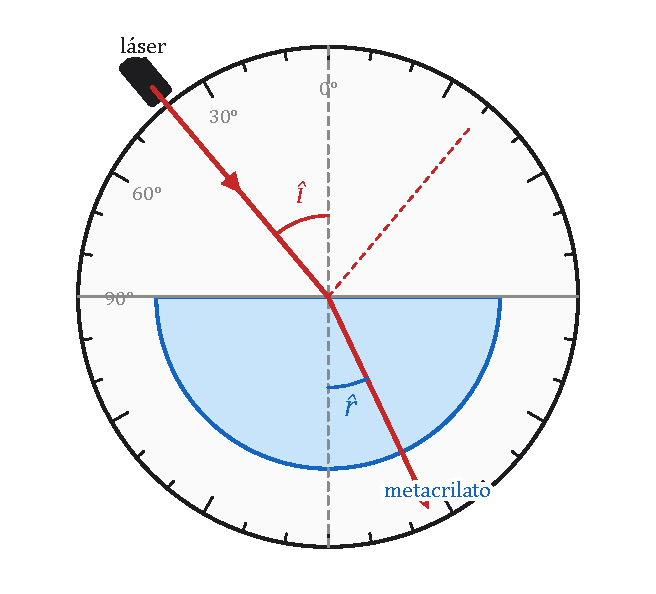
\includegraphics[width=\linewidth]{images/UD3/practica_snell}
    \captionof{figure}{Medida de los ángulos.}
    \label{fig:opt-practica-snell}
\end{minipage}

\begin{table}[H]
    \centering
    \caption{Datos de la práctica de la ley de Snell}
    \vspace{-5pt}
    \begin{tabular}{@{}C{2.4cm}C{2.4cm}C{2.4cm}C{2.4cm}C{2.6cm}@{}}
        \toprule
        \textbf{\(\hat{\imath}\) (\unit{\degree})} & \textbf{\(\hat r\) (\unit{\degree})} & \textbf{\(\sen\hat{\imath}\)} & \textbf{\(\sen\hat r\)} & \textbf{\(n = \sen\hat{\imath}/\sen\hat r\)} \\
        \midrule
        \rule{0pt}{18pt} & & & & \\ \midrule[0.3pt]
        \rule{0pt}{18pt} & & & & \\ \midrule[0.3pt]
        \rule{0pt}{18pt} & & & & \\ \midrule[0.3pt]
        \rule{0pt}{18pt} & & & & \\
        \bottomrule
    \end{tabular}
    \label{tab:opt-practica-snell}
\end{table}

\textbf{Cálculos.} Representa \(\sen\hat{\imath}\) frente a \(\sen\hat r\): debe salir una recta que pasa por el origen y
cuya pendiente es \(n\).

\textbf{Cuestiones.}
\begin{enumerate}[label=\letraminuscula]
    \item Con el índice obtenido, calcula el ángulo límite teórico y compáralo con el medido.
    \item ¿Por qué hay que hacer llegar el rayo al centro de la cara plana?
    \item ¿Qué observas en el rayo reflejado a medida que te acercas al ángulo límite?
\end{enumerate}

\subsection{Práctica 2: distancia focal de una lente convergente}\label{subsec:opt-practica-lente}

\textbf{Objetivo.} Medir la distancia focal de una lente convergente con el banco óptico y comprobar la ecuación de las
lentes.

\textbf{Material.} Banco óptico con regla, lámpara, objeto (una flecha o una letra recortada en una cartulina), lente
convergente con soporte y pantalla.

\begin{figure}[H]
    \centering
    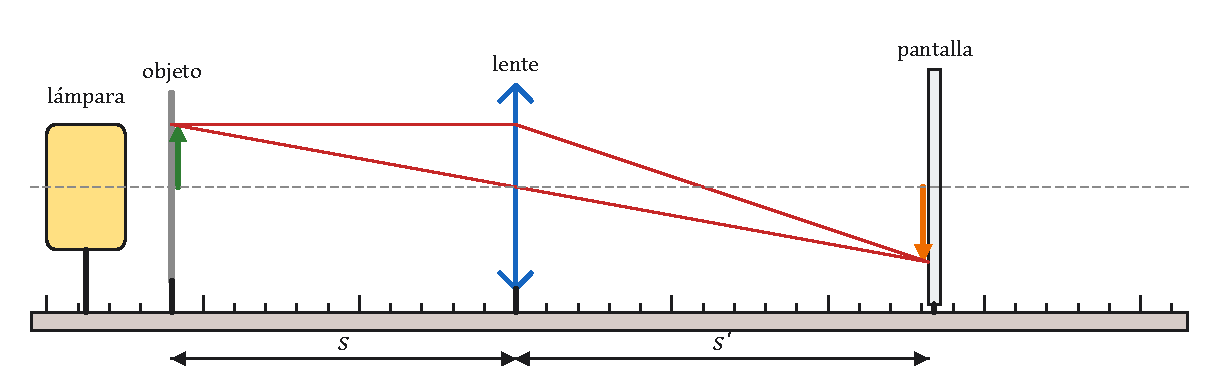
\includegraphics[width=0.85\linewidth]{images/UD3/practica_lente}
    \caption{Montaje en el banco óptico. Se mueve la pantalla hasta que la imagen se ve nítida.}
    \label{fig:opt-practica-lente}
\end{figure}

\textbf{Procedimiento.}
\begin{enumerate}[label=\numberballmDarkTeal]
    \item Estimación rápida: enfoca con la lente la imagen de una ventana lejana sobre una pared. La distancia de la lente
    a la pared es, aproximadamente, \(f'\).
    \item Monta el banco (figura~\ref{fig:opt-practica-lente}). Coloca el objeto a una distancia \(|s|\) mayor que \(f'\) y
    mueve la pantalla hasta ver la imagen nítida. Mide \(s\), \(s'\) y el tamaño de la imagen.
    \item Repite para al menos cuatro distancias distintas.
\end{enumerate}

\begin{table}[H]
    \centering
    \caption{Datos de la práctica de la lente convergente}
    \vspace{-5pt}
    \begin{tabular}{@{}C{2.2cm}C{2.2cm}C{2.4cm}C{2.4cm}C{2.4cm}C{2cm}@{}}
        \toprule
        \textbf{\(s\) (\unit{\cm})} & \textbf{\(s'\) (\unit{\cm})} & \textbf{\(1/s\) (\unit{\per\cm})} & \textbf{\(1/s'\) (\unit{\per\cm})} & \textbf{\(f'\) (\unit{\cm})} & \textbf{\(\beta\)} \\
        \midrule
        \rule{0pt}{18pt} & & & & & \\ \midrule[0.3pt]
        \rule{0pt}{18pt} & & & & & \\ \midrule[0.3pt]
        \rule{0pt}{18pt} & & & & & \\ \midrule[0.3pt]
        \rule{0pt}{18pt} & & & & & \\
        \bottomrule
    \end{tabular}
    \label{tab:opt-practica-lente}
\end{table}

\textbf{Cálculos.} Con cada pareja calcula \(f'\) con \(1/f' = 1/s' - 1/s\) (recuerda que \(s < 0\)) y halla la media.
Método gráfico: representa \(1/s'\) frente a \(1/s\); es una recta de pendiente 1 cuya ordenada en el origen es \(1/f'\).

\textbf{Cuestiones.}
\begin{enumerate}[label=\letraminuscula]
    \item Compara el aumento medido (\(y'/y\)) con el calculado (\(s'/s\)).
    \item ¿Qué pasa si colocas el objeto entre el foco y la lente? ¿Puedes recoger la imagen en la pantalla? ¿Por qué?
    \item Calcula la potencia de la lente en dioptrías.
\end{enumerate}


    \newpage

    %! Unidad 3 — Óptica geométrica: ejercicios finales (adaptados de la fuente, con datos cambiados y resueltos)

\section{Ejercicios}\label{sec:opt-ejercicios}

\subsection{Naturaleza de la luz, reflexión y refracción}

\begin{exercise}
    ¿Cuál es la frecuencia de una luz que en el aire tiene una longitud de onda de \qty{600}{\nm}? ¿Cuál es su frecuencia, su
    velocidad y su longitud de onda en el agua (\(n = 1{,}33\))?
    \begin{solu}
        \(\nu = \dfrac{c}{\lambda} = \dfrac{3\cdot 10^8}{600\cdot 10^{-9}} = \textcolor{red}{\qty{5e14}{\hertz}}\); \textcolor{red}{en el agua es la misma}.

        \(v = \dfrac{c}{n} = \textcolor{red}{\qty{2.26e8}{\m\per\second}}\); \(\lambda = \dfrac{600}{1{,}33} = \textcolor{red}{\qty{451}{\nm}}\).
    \end{solu}
\end{exercise}

\begin{exercise}
    Un rayo que viaja por el aire llega a la superficie de un estanque con un ángulo de incidencia de \ang{40}
    (\(n_{\text{agua}} = 1{,}33\)).
    \begin{enumerate}[label=\letraminuscula]
        \item ¿Qué ángulo forman entre sí el rayo reflejado y el refractado?
        \item Si la luz fuera del agua al aire, ¿a partir de qué ángulo de incidencia habría reflexión total?
    \end{enumerate}
    \begin{solu}
        \begin{enumerate}[label=\letraminuscula]
            \item \(\sen\hat r = \dfrac{\sen\ang{40}}{1{,}33} \Rightarrow \hat r = \ang{28.9}\).
            \textcolor{blue}{El reflejado forma \ang{40} con la normal por arriba y el refractado \ang{28.9} por abajo:}
            \(\ang{180} - \ang{40} - \ang{28.9} = \textcolor{red}{\ang{111.1}}\).
            \item \(\sen\hat{\imath}_L = \dfrac{1}{1{,}33} \Rightarrow \textcolor{red}{\hat{\imath}_L = \ang{48.8}}\).
        \end{enumerate}
    \end{solu}
\end{exercise}

\begin{exercise}
    Cuando un rayo incide sobre cierto material con un ángulo de \ang{35}, los rayos reflejado y refractado forman entre sí
    \ang{125}. Calcula el índice de refracción del material.
    \begin{solu}
        \textcolor{blue}{\(\ang{180} = \hat{\imath} + \ang{125} + \hat r \Rightarrow \hat r = \ang{20}\).}
        \(n = \dfrac{\sen\ang{35}}{\sen\ang{20}} = \textcolor{red}{1{,}68}\).
    \end{solu}
\end{exercise}

\begin{exercise}
    El índice de refracción del agua es \num{1.33} y el de un vidrio \emph{flint}, \num{1.60}. Calcula el ángulo límite entre
    los dos medios. ¿En qué sentido debe ir la luz para que pueda haber reflexión total?
    \begin{solu}
        \(\sen\hat{\imath}_L = \dfrac{1{,}33}{1{,}60} = 0{,}831 \Rightarrow \textcolor{red}{\hat{\imath}_L = \ang{56.2}}\).
        \textcolor{red}{Del vidrio hacia el agua} \textcolor{blue}{(de más a menos refringente).}
    \end{solu}
\end{exercise}

\begin{exercise}
    Si un rayo de luz pasa del etanol (\(n = 1{,}36\)) al aire, ¿a partir de qué ángulo de incidencia hay reflexión total?
    \begin{solu}
        \(\sen\hat{\imath}_L = \dfrac{1}{1{,}36} \Rightarrow \textcolor{red}{\hat{\imath}_L = \ang{47.3}}\).
    \end{solu}
\end{exercise}

\begin{exercise}
    Un cubo de vidrio (\(n = 1{,}6\)) está sumergido en agua (\(n = 1{,}33\)). Un rayo entra por una cara lateral y llega a
    la cara superior. ¿Qué ángulo de incidencia en la cara lateral, como máximo, hace falta para que en la cara superior se
    produzca reflexión total?
    \begin{solu}
        \textcolor{blue}{Ángulo límite vidrio-agua: \(\sen\hat{\imath}_L = 1{,}33/1{,}6 \Rightarrow \hat{\imath}_L = \ang{56.2}\).
        Las dos caras son perpendiculares, así que el ángulo con que el rayo llega a la cara superior es \(\ang{90} - \hat r\),
        donde \(\hat r\) es el de refracción en la lateral. Para reflexión total: \(\ang{90} - \hat r \geq \ang{56.2} \Rightarrow \hat r \leq \ang{33.8}\).}
        \[ \sen\hat{\imath} \leq \dfrac{1{,}6}{1{,}33}\sen\ang{33.8} = 0{,}669 \;\Rightarrow\; \textcolor{red}{\hat{\imath} \leq \ang{42.0}} \]
    \end{solu}
\end{exercise}

\begin{exercise}
    En el laboratorio se hace llegar un rayo de luz a la cara plana de un semicilindro de vidrio con distintos ángulos de
    incidencia y se miden los de refracción:
    \begin{center}
        \begin{tabular}{@{}lcccc@{}}
            \toprule
            \(\hat{\imath}\) & \ang{15} & \ang{30} & \ang{45} & \ang{60} \\
            \midrule
            \(\hat r\) & \ang{10.0} & \ang{19.6} & \ang{28.3} & \ang{35.5} \\
            \bottomrule
        \end{tabular}
    \end{center}
    Calcula el índice de refracción del vidrio, la velocidad de la luz en él y su ángulo límite.
    \begin{solu}
        \textcolor{blue}{\(n = \sen\hat{\imath}/\sen\hat r\) en cada medida: \num{1.49}; \num{1.49}; \num{1.49}; \num{1.49}.}
        \(n = \textcolor{red}{1{,}49}\); \(v = \dfrac{c}{n} = \textcolor{red}{\qty{2.01e8}{\m\per\second}}\);
        \(\sen\hat{\imath}_L = \dfrac{1}{1{,}49} \Rightarrow \textcolor{red}{\hat{\imath}_L = \ang{42.2}}\).
    \end{solu}
\end{exercise}

\subsection{Lámina y prisma}

\begin{exercise}
    Una lámina de vidrio de caras paralelas, situada en el aire, tiene \qty{6}{\cm} de espesor e índice \num{1.58}. Un rayo
    incide en ella con un ángulo de \ang{35}. Calcula:
    \begin{enumerate}[label=\letraminuscula]
        \item El ángulo de refracción dentro de la lámina y el de emergencia.
        \item El desplazamiento lateral del rayo y la distancia que recorre dentro de la lámina.
    \end{enumerate}
    \begin{solu}
        \begin{enumerate}[label=\letraminuscula]
            \item \(\sen\hat r = \dfrac{\sen\ang{35}}{1{,}58} \Rightarrow \textcolor{red}{\hat r = \ang{21.3}}\); \textcolor{red}{emerge con \ang{35}}.
            \item \(AB = \dfrac{6}{\cos\ang{21.3}} = \textcolor{red}{\qty{6.44}{\cm}}\);
            \(\delta = 6{,}44\sen(\ang{35} - \ang{21.3}) = \textcolor{red}{\qty{1.53}{\cm}}\).
        \end{enumerate}
    \end{solu}
\end{exercise}

\begin{exercise}
    Sobre una cara de un prisma de vidrio (\(n = 1{,}5\)) de ángulo \ang{50}, situado en el aire, incide un rayo con un
    ángulo de \ang{25}. Calcula el ángulo de emergencia, la desviación y la desviación mínima del prisma.
    \begin{solu}
        \textcolor{blue}{Primera cara:} \(\sen\hat r_1 = \dfrac{\sen\ang{25}}{1{,}5} \Rightarrow \hat r_1 = \ang{16.4}\).
        \textcolor{blue}{Segunda cara:} \(\hat{\imath}_2 = \varphi - \hat r_1 = \ang{33.6}\);
        \(\sen\hat r_2 = 1{,}5\sen\ang{33.6} \Rightarrow \textcolor{red}{\hat r_2 = \ang{56.2}}\).

        \(\delta = \hat{\imath}_1 + \hat r_2 - \varphi = 25 + 56{,}2 - 50 = \textcolor{red}{\ang{31.2}}\).

        \textcolor{blue}{Desviación mínima: \(\hat r_1 = \ang{25}\), \(\sen\hat{\imath}_1 = 1{,}5\sen\ang{25} \Rightarrow \hat{\imath}_1 = \ang{39.3}\);}
        \(\delta_m = 2\cdot\ang{39.3} - \ang{50} = \textcolor{red}{\ang{28.7}}\).
    \end{solu}
\end{exercise}

\begin{exercise}
    Un prisma de \ang{60} produce una desviación mínima de \ang{40}. Calcula el índice de refracción del material y el
    ángulo de incidencia que da esa desviación.
    \begin{solu}
        \(n = \dfrac{\sen\dfrac{40 + 60}{2}}{\sen 30} = \dfrac{\sen\ang{50}}{\sen\ang{30}} = \textcolor{red}{1{,}53}\);
        \(\hat{\imath}_1 = \dfrac{\delta_m + \varphi}{2} = \textcolor{red}{\ang{50}}\).
    \end{solu}
\end{exercise}

\begin{exercise}
    En un prisma de \ang{40}, un rayo que incide con un ángulo de \ang{31} recorre el interior del prisma paralelo a su base.
    Calcula el índice de refracción del prisma.
    \begin{solu}
        \textcolor{blue}{Si el rayo interior es paralelo a la base, la marcha es simétrica: \(\hat r_1 = \varphi/2 = \ang{20}\).}
        \(n = \dfrac{\sen\ang{31}}{\sen\ang{20}} = \textcolor{red}{1{,}51}\).
    \end{solu}
\end{exercise}

\subsection{Dioptrios y espejos}

\begin{exercise}
    Una piscina parece tener \qty{1.5}{\m} de profundidad. ¿Cuál es su profundidad real? (\(n_{\text{agua}} = 1{,}33\)).
    \begin{solu}
        \(\dfrac{s'}{s} = \dfrac{n'}{n} = \dfrac{1}{1{,}33} \Rightarrow s = 1{,}33\cdot 1{,}5 = \textcolor{red}{\qty{2.0}{\m}}\).
    \end{solu}
\end{exercise}

\begin{exercise}
    Un objeto de \qty{15}{\mm} está a \qty{12}{\cm} del vértice de un espejo convexo de \qty{30}{\cm} de radio. ¿Dónde se
    forma la imagen y cómo es?
    \begin{solu}
        \textcolor{blue}{\(f = R/2 = \qty{15}{\cm}\).} \(\dfrac{1}{s'} = \dfrac{1}{15} + \dfrac{1}{12} \Rightarrow \textcolor{red}{s' = \qty{6.67}{\cm}}\);
        \(\beta = -\dfrac{6{,}67}{-12} = 0{,}556 \Rightarrow \textcolor{red}{y' = \qty{8.3}{\mm}}\).
        \textcolor{red}{Virtual, derecha y menor.}
    \end{solu}
\end{exercise}

\begin{exercise}
    Un objeto de \qty{2}{\cm} está a \qty{24}{\cm} del vértice de un espejo cóncavo de \qty{16}{\cm} de radio. ¿Dónde está
    la imagen y qué características tiene? Dibuja el esquema de rayos.
    \begin{solu}
        \textcolor{blue}{\(f = \qty{-8}{\cm}\).} \(\dfrac{1}{s'} = \dfrac{1}{-8} - \dfrac{1}{-24} = -\dfrac{1}{12} \Rightarrow \textcolor{red}{s' = \qty{-12}{\cm}}\);
        \(\beta = -0{,}5 \Rightarrow \textcolor{red}{y' = \qty{-1}{\cm}}\).
        \textcolor{red}{Real, invertida y menor} \textcolor{blue}{(el objeto está más allá de \(C\), como en la figura~\ref{fig:opt-espejos-imagenes}a).}
    \end{solu}
\end{exercise}

\begin{exercise}
    Un espejo situado a \qty{1.5}{\m} de un objeto da una imagen derecha y cuatro veces mayor. ¿Es cóncavo o convexo?
    ¿Cuánto mide su radio de curvatura?
    \begin{solu}
        \textcolor{blue}{Una imagen derecha y mayor solo la da un espejo cóncavo con el objeto entre el foco y el espejo.}
        \(\beta = -\dfrac{s'}{s} = 4 \Rightarrow s' = -4s = \qty{600}{\cm}\).
        \[ \dfrac{1}{f} = \dfrac{1}{600} + \dfrac{1}{-150} = -\dfrac{3}{600} \;\Rightarrow\; f = \qty{-200}{\cm} \]
        \textcolor{red}{Cóncavo, de radio \(R = 2f = \qty{-4}{\m}\).}
    \end{solu}
\end{exercise}

\begin{exercise}
    ¿Qué características tiene la imagen que da un espejo esférico si la distancia imagen es negativa y el aumento lateral
    también?
    \begin{solu}
        \textcolor{red}{\(s' < 0\): la imagen está delante del espejo y es real. \(\beta < 0\): es invertida.}
        \textcolor{blue}{Solo puede darla un espejo cóncavo con el objeto más allá del foco.}
    \end{solu}
\end{exercise}

\begin{exercise}
    Tenemos un espejo cóncavo de \qty{1}{\m} de radio. ¿Dónde hay que poner un objeto pequeño para obtener una imagen
    invertida y tres veces mayor?
    \begin{solu}
        \textcolor{blue}{\(f = \qty{-50}{\cm}\). Invertida: \(\beta = -\dfrac{s'}{s} = -3 \Rightarrow s' = 3s\).}
        \[ \dfrac{1}{3s} + \dfrac{1}{s} = \dfrac{1}{-50} \;\Rightarrow\; \dfrac{4}{3s} = -\dfrac{1}{50} \;\Rightarrow\; \textcolor{red}{s = \qty{-66.7}{\cm}} \]
        \textcolor{blue}{(Entre \(C\) y \(F\); la imagen, real, está a \qty{2}{\m} del espejo.)}
    \end{solu}
\end{exercise}

\begin{exercise}
    Un espejo cóncavo forma una imagen real tres veces mayor que el objeto, que está a \qty{30}{\cm} del espejo. Calcula el
    radio de curvatura.
    \begin{solu}
        \textcolor{blue}{Real: invertida, \(\beta = -3 \Rightarrow s' = 3s = \qty{-90}{\cm}\).}
        \(\dfrac{1}{f} = \dfrac{1}{-90} + \dfrac{1}{-30} = -\dfrac{4}{90} \Rightarrow f = \qty{-22.5}{\cm}\);
        \(\textcolor{red}{R = \qty{-45}{\cm}}\).
    \end{solu}
\end{exercise}

\subsection{Lentes}

\begin{exercise}
    Un objeto de \qty{1.5}{\cm} se coloca a \qty{20}{\cm} de una lente convergente de \qty{30}{\cm} de distancia focal.
    Calcula la posición y el tamaño de la imagen.
    \begin{solu}
        \(\dfrac{1}{s'} = \dfrac{1}{30} + \dfrac{1}{-20} = -\dfrac{1}{60} \Rightarrow \textcolor{red}{s' = \qty{-60}{\cm}}\);
        \(\beta = \dfrac{-60}{-20} = 3 \Rightarrow \textcolor{red}{y' = \qty{4.5}{\cm}}\).
        \textcolor{red}{Virtual, derecha y mayor} \textcolor{blue}{(actúa como lupa).}
    \end{solu}
\end{exercise}

\begin{exercise}
    Dibuja el esquema de rayos de la imagen que da una lente convergente de distancia focal \(f'\) cuando el objeto está:
    a) a menos de \(f'\); b) a más de \(2f'\); c) entre \(f'\) y \(2f'\). Indica las características de cada imagen.
    \begin{solu}
        \textcolor{blue}{Ver la figura~\ref{fig:opt-lentes-imagenes}.}
        \begin{enumerate}[label=\letraminuscula]
            \item \textcolor{red}{Virtual, derecha y mayor}, del mismo lado que el objeto.
            \item \textcolor{red}{Real, invertida y menor}, entre \(F'\) y \(2F'\).
            \item \textcolor{red}{Real, invertida y mayor}, más allá de \(2F'\).
        \end{enumerate}
    \end{solu}
\end{exercise}

\begin{exercise}
    Construye la imagen de un objeto situado más allá del foco de una lente divergente. ¿Cambian sus características si el
    objeto está entre el foco y la lente?
    \begin{solu}
        \textcolor{blue}{El rayo paralelo al eje sale como si viniera de \(F'\) (que está delante de la lente) y el que pasa por
        el centro no se desvía. Sus prolongaciones se cortan entre \(F'\) y la lente.}
        \textcolor{red}{La imagen es siempre virtual, derecha y menor, esté donde esté el objeto.}
    \end{solu}
\end{exercise}

\begin{exercise}
    ¿Qué aumento produce una lente convergente de \qty{12}{\cm} de distancia focal si el objeto está a \qty{4}{\cm} de ella?
    \begin{solu}
        \(\dfrac{1}{s'} = \dfrac{1}{12} - \dfrac{1}{4} = -\dfrac{1}{6} \Rightarrow s' = \qty{-6}{\cm}\);
        \(\beta = \dfrac{-6}{-4} = \textcolor{red}{1{,}5}\) \textcolor{blue}{(imagen virtual y derecha).}
    \end{solu}
\end{exercise}

\begin{exercise}
    Un objeto de \qty{2}{\cm} está a \qty{15}{\cm} de una lente divergente de \qty{25}{\cm} de distancia focal. Calcula la
    posición y el tamaño de la imagen.
    \begin{solu}
        \textcolor{blue}{\(f' = \qty{-25}{\cm}\).} \(\dfrac{1}{s'} = -\dfrac{1}{25} - \dfrac{1}{15} \Rightarrow \textcolor{red}{s' = \qty{-9.4}{\cm}}\);
        \(\beta = 0{,}625 \Rightarrow \textcolor{red}{y' = \qty{1.25}{\cm}}\): \textcolor{red}{virtual, derecha y menor}.
    \end{solu}
\end{exercise}

\begin{exercise}
    La imagen real de un objeto, invertida y tres veces mayor, se forma a \qty{30}{\cm} de una lente convergente. Calcula
    la potencia de la lente.
    \begin{solu}
        \textcolor{blue}{\(\beta = \dfrac{s'}{s} = -3\) con \(s' = \qty{30}{\cm} \Rightarrow s = \qty{-10}{\cm}\).}
        \(\dfrac{1}{f'} = \dfrac{1}{30} - \dfrac{1}{-10} = \dfrac{4}{30} \Rightarrow f' = \qty{7.5}{\cm}\);
        \(P = \dfrac{1}{0{,}075} = \textcolor{red}{\qty{13.3}{D}}\).
    \end{solu}
\end{exercise}

\begin{exercise}
    Un objeto de \qty{2}{\cm} está a \qty{30}{\cm} de una lente de \qty{-5}{D}. Calcula la distancia focal, la posición, el
    tamaño y las características de la imagen, y construye el diagrama de rayos.
    \begin{solu}
        \(f' = \dfrac{1}{-5} = \textcolor{red}{\qty{-20}{\cm}}\) \textcolor{blue}{(divergente).}
        \(\dfrac{1}{s'} = -\dfrac{1}{20} - \dfrac{1}{30} \Rightarrow \textcolor{red}{s' = \qty{-12}{\cm}}\);
        \(\beta = 0{,}4 \Rightarrow \textcolor{red}{y' = \qty{0.8}{\cm}}\): \textcolor{red}{virtual, derecha y menor}
        \textcolor{blue}{(como en la figura~\ref{fig:opt-lentes-imagenes}d).}
    \end{solu}
\end{exercise}

\begin{exercise}
    Dos lentes convergentes delgadas, de \qty{8}{\cm} y \qty{12}{\cm} de distancia focal, están separadas \qty{50}{\cm}. Un
    objeto de \qty{3}{\cm} se coloca \qty{24}{\cm} delante de la primera. Calcula la posición y el tamaño de la imagen final.
    \begin{solu}
        \textcolor{blue}{Primera lente:} \(\dfrac{1}{s'_1} = \dfrac{1}{8} - \dfrac{1}{24} \Rightarrow s'_1 = \qty{12}{\cm}\); \(\beta_1 = \dfrac{12}{-24} = -0{,}5\).

        \textcolor{blue}{Esa imagen hace de objeto para la segunda, a \(50 - 12 = \qty{38}{\cm}\) delante de ella: \(s_2 = \qty{-38}{\cm}\).}
        \(\dfrac{1}{s'_2} = \dfrac{1}{12} - \dfrac{1}{38} \Rightarrow \textcolor{red}{s'_2 = \qty{17.5}{\cm}}\) \textcolor{blue}{detrás de la segunda lente}; \(\beta_2 = -0{,}46\).

        \(\beta = \beta_1\beta_2 = 0{,}23 \Rightarrow \textcolor{red}{y' = \qty{0.69}{\cm}}\): \textcolor{red}{real, derecha y menor}.
    \end{solu}
\end{exercise}

\begin{exercise}
    Una lente planoconvexa de vidrio (\(n = 1{,}5\)) tiene una distancia focal de \qty{40}{\cm}. ¿Cuál es el radio de su cara
    curva? ¿Y su potencia?
    \begin{solu}
        \textcolor{blue}{Con \(R_2 = \infty\):} \(\dfrac{1}{40} = 0{,}5\cdot\dfrac{1}{R_1} \Rightarrow \textcolor{red}{R_1 = \qty{20}{\cm}}\);
        \(P = \dfrac{1}{0{,}40} = \textcolor{red}{\qty{2.5}{D}}\).
    \end{solu}
\end{exercise}

\begin{exercise}
    El punto próximo de una persona con presbicia está a \qty{1}{\m}. ¿Qué potencia deben tener sus gafas para leer a
    \qty{25}{\cm}?
    \begin{solu}
        \textcolor{blue}{El texto (\(s = \qty{-0.25}{\m}\)) debe dar una imagen virtual en el punto próximo (\(s' = \qty{-1}{\m}\)):}
        \(P = \dfrac{1}{s'} - \dfrac{1}{s} = -1 + 4 = \textcolor{red}{\qty{3}{D}}\) \textcolor{blue}{(convergente).}
    \end{solu}
\end{exercise}


%----------------------------------------------------------------------------------------
%	PARTE: INTERACCIÓN GRAVITATORIA
%----------------------------------------------------------------------------------------

    \part{Interacción gravitatoria}

    \chapterimage{images/portada_cabeceras/cabecera_UD4}
    \chapter{Interacción gravitatoria}

    %! Unidad 4 — Interacción gravitatoria (teoría, actividades resueltas y prácticas)
%! Fuente: Fuentes/Tema_4.pdf (reescrito; datos de las actividades cambiados y recalculados)

\section*{Para empezar: la manzana y la Luna}
\addcontentsline{toc}{section}{Para empezar: la manzana y la Luna}

Cuenta la leyenda que Isaac Newton, viendo caer una manzana, se preguntó si la fuerza que la hacía caer era la misma que
mantenía a la Luna girando alrededor de la Tierra. Hizo la cuenta: la Luna está unas 60 veces más lejos del centro de la
Tierra que la manzana, y su aceleración hacia la Tierra resulta ser unas \(60^2 = 3600\) veces menor que \(g\). Era la misma
fuerza, debilitada con el cuadrado de la distancia. Con esa idea unificó por primera vez la física «de la Tierra» y la «del
cielo». En esta unidad recorreremos ese camino: desde las leyes de Kepler hasta la ley de la gravitación universal, el
concepto de campo y el movimiento de planetas y satélites.

\section{Modelos del universo}\label{sec:grav-modelos}

\paragraph{Modelos geocéntricos.} En la Antigüedad se pensaba que la Tierra estaba inmóvil en el centro del universo y que
todos los astros, también el Sol, giraban a su alrededor. Para \textbf{Aristóteles} (siglo \textsc{iv} a.\,C.) el universo
tenía dos regiones: la \emph{sublunar}, formada por los cuatro elementos (tierra, agua, aire y fuego), donde todo cambia, y
la \emph{celeste}, donde los astros se movían en esferas concéntricas con movimientos circulares, uniformes y eternos.

\textbf{Ptolomeo} (siglo \textsc{ii}) perfeccionó el modelo para explicar que los planetas a veces parecen retroceder en el
cielo: cada planeta gira en un círculo pequeño, el \azuln{epiciclo}, cuyo centro gira a su vez alrededor de la Tierra en un
círculo mayor, el \azuln{deferente} (figura~\ref{fig:grav-modelos}). Este modelo se usó durante casi 1500 años.

\paragraph{Modelos heliocéntricos.} En 1543 \textbf{Copérnico} propuso que el Sol está en el centro y que la Tierra es un
planeta más, que gira sobre sí misma y alrededor del Sol. La idea chocaba con la interpretación de la época de las Sagradas
Escrituras y tardó en aceptarse. \textbf{Galileo} la defendió con las observaciones de su telescopio (las lunas de Júpiter,
las fases de Venus), lo que le costó un proceso de la Inquisición en 1633. Las medidas muy precisas del danés
\textbf{Tycho Brahe} permitieron a su ayudante \textbf{Kepler} enunciar las leyes del movimiento planetario, y con ellas el
modelo heliocéntrico quedó establecido.

\begin{figure}[H]
    \centering
    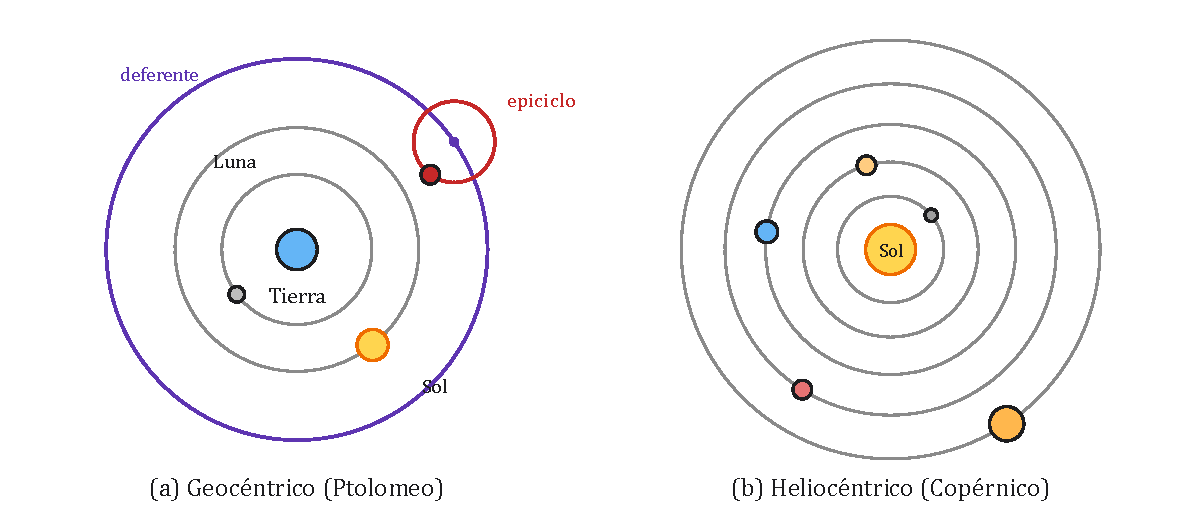
\includegraphics[width=0.88\linewidth]{images/UD4/modelos}
    \caption{(a) En el modelo de Ptolomeo, Marte gira en un epiciclo cuyo centro recorre el deferente alrededor de la Tierra.
    (b) En el de Copérnico, los planetas giran alrededor del Sol.}
    \label{fig:grav-modelos}
\end{figure}

\section{Las leyes de Kepler}\label{sec:grav-kepler}

Kepler dedicó años a analizar las observaciones de Brahe sobre Marte y llegó a tres leyes \emph{empíricas} (deducidas de
los datos, sin explicar su causa):

\begin{definition}[Leyes de Kepler]
    \begin{enumerate}[label=\numberballmDarkTeal]
        \item \rojon{Ley de las órbitas}. Los planetas describen órbitas elípticas, con el Sol en uno de sus focos.
        \item \rojon{Ley de las áreas}. El radio vector que une el Sol con un planeta barre áreas iguales en tiempos iguales:
        la \azuln{velocidad areolar} \(dA/dt\) es constante.
        \item \rojon{Ley de los períodos}. Los cuadrados de los períodos de revolución son proporcionales a los cubos de los
        semiejes mayores de las órbitas (o de los radios medios):
        \begin{centeredequation}
            \boxed{\dfrac{T^2}{r^3} = \text{constante}} \qquad\Rightarrow\qquad \dfrac{T_1^2}{r_1^3} = \dfrac{T_2^2}{r_2^3} \label{eq:grav-kepler3}
        \end{centeredequation}
    \end{enumerate}
\end{definition}

\begin{figure}[H]
    \centering
    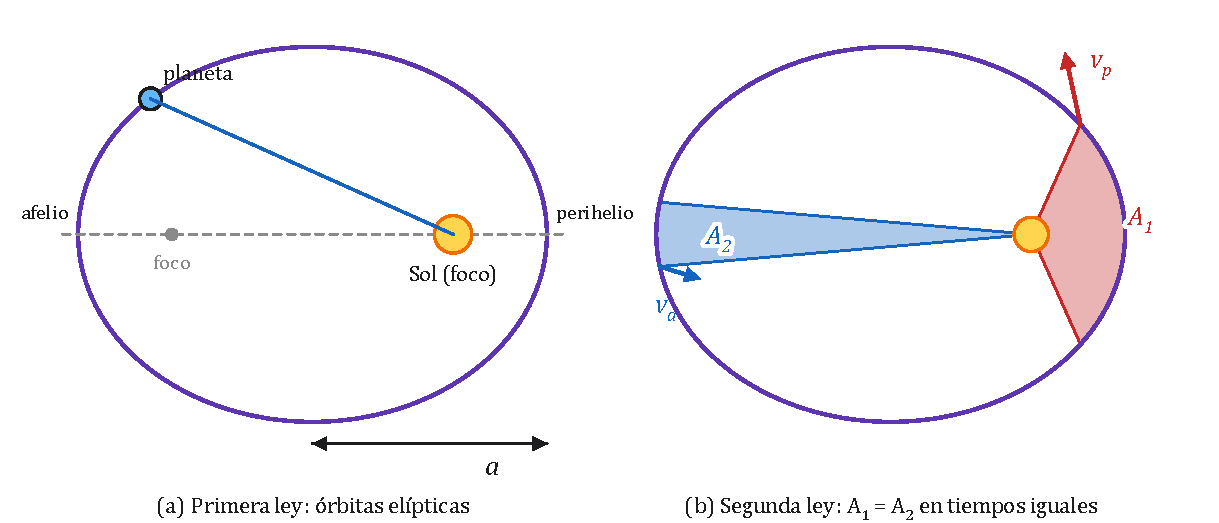
\includegraphics[width=0.95\linewidth]{images/UD4/kepler}
    \caption{(a) Órbita elíptica (muy exagerada: las órbitas de los planetas son casi circulares). (b) Las dos zonas
    sombreadas se barren en el mismo tiempo: cerca del Sol el planeta va más deprisa.}
    \label{fig:grav-kepler}
\end{figure}

El punto de la órbita más cercano al Sol es el \azuln{perihelio} y el más lejano, el \azuln{afelio} (para la Tierra,
\emph{perigeo} y \emph{apogeo}). Las tres leyes valen también para cualquier conjunto de satélites que giran alrededor de un
mismo astro central (las lunas de Júpiter, los satélites artificiales de la Tierra), pero con una constante distinta en la
tercera ley para cada astro central.

\begin{exercise}
    Ío, una de las lunas de Júpiter, gira en una órbita de \qty{4.22e5}{\km} de radio con un período de \qty{1.77}{días}.
    Europa gira a \qty{6.71e5}{\km}. ¿Cuál es el período de Europa?
    \begin{solu}
        \textcolor{blue}{Las dos giran alrededor de Júpiter: misma constante en la tercera ley.}
        \[ T_E = T_I\left(\dfrac{r_E}{r_I}\right)^{3/2} = 1{,}77\left(\dfrac{6{,}71}{4{,}22}\right)^{3/2} = \textcolor{red}{\qty{3.55}{días}} \]
    \end{solu}
\end{exercise}

\section{Momento angular}\label{sec:grav-momento}

Para justificar las dos primeras leyes de Kepler necesitamos una nueva magnitud.

\begin{definition}[Momento angular]
    El \rojon{momento angular} (o cinético) de una partícula de masa \(m\) y velocidad \(\vec v\) respecto de un punto \(O\) es:
    \begin{centeredequation}
        \boxed{\vec L = \vec r \times \vec p = \vec r \times m\vec v} \label{eq:grav-L}
    \end{centeredequation}
    donde \(\vec r\) es el vector de posición de la partícula respecto de \(O\). Se mide en \unit{\kg\m\squared\per\second}.
\end{definition}

Por ser un producto vectorial, \(\vec L\) es perpendicular al plano que forman \(\vec r\) y \(\vec v\); su sentido es el de
avance de un sacacorchos que gira llevando \(\vec r\) hacia \(\vec v\) por el camino más corto, y su módulo es
\(L = r\,m\,v\sen\varphi\) (figura~\ref{fig:grav-L}).

\begin{figure}[H]
    \centering
    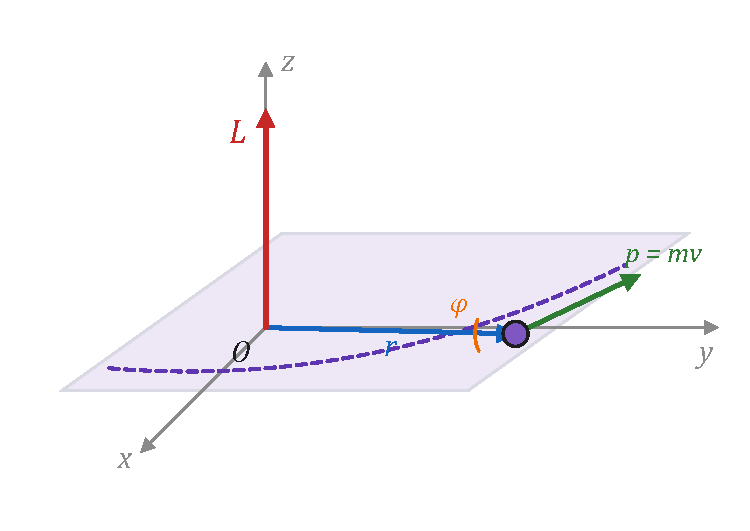
\includegraphics[width=0.48\linewidth]{images/UD4/momento_angular}
    \caption{El momento angular es perpendicular al plano en el que se mueve la partícula.}
    \label{fig:grav-L}
\end{figure}

\paragraph{Conservación del momento angular.} Derivando respecto del tiempo:
\begin{equation*}
    \dfrac{d\vec L}{dt} = \dfrac{d\vec r}{dt}\times m\vec v + \vec r\times\dfrac{d(m\vec v)}{dt} = \underbrace{\vec v\times m\vec v}_{0} + \vec r\times\vec F = \vec M
\end{equation*}
El primer término es nulo porque los dos vectores son paralelos; el segundo es el \azuln{momento de la fuerza}
\(\vec M = \vec r\times\vec F\).
\begin{remark}
    Si el momento de la fuerza que actúa sobre una partícula respecto de un punto es nulo, el momento angular respecto de ese
    punto \textbf{se conserva} (es constante en módulo, dirección y sentido).
\end{remark}

\paragraph{Fuerzas centrales.} Una fuerza es \rojon{central} si está siempre dirigida hacia un mismo punto, el
\emph{centro de fuerzas}. La atracción del Sol sobre un planeta es central. Como \(\vec F\) es paralela a \(\vec r\),
\(\vec M = \vec r \times\vec F = 0\): \textbf{bajo una fuerza central el momento angular se conserva}.

\paragraph{Justificación de las dos primeras leyes de Kepler.}
\begin{itemize}
    \item Como \(\vec L\) tiene dirección constante y es perpendicular a \(\vec r\) y \(\vec v\), el planeta se mueve
    siempre en el mismo plano: la órbita es una \textbf{curva plana} (Newton demostró después que es una elipse).
    \item En un tiempo \(dt\) el radio vector barre un triángulo de área \(dA = \frac{1}{2}\,r\,v\,dt\sen\varphi\). Como
    \(L = r\,m\,v\sen\varphi\):
    \begin{centeredequation}
        \dfrac{dA}{dt} = \dfrac{1}{2}\,r\,v\sen\varphi = \boxed{\dfrac{L}{2m}} = \text{constante} \label{eq:grav-areolar}
    \end{centeredequation}
    la velocidad areolar es constante: es la segunda ley.
\end{itemize}
En el perihelio y en el afelio la velocidad es perpendicular al radio vector (\(\sen\varphi = 1\)), y la conservación de
\(L\) da \(m\,r_p v_p = m\,r_a v_a\), es decir:
\begin{centeredequation}
    \boxed{r_p\,v_p = r_a\,v_a} \label{eq:grav-perihelio}
\end{centeredequation}
El planeta va más deprisa en el perihelio. En una órbita circular la velocidad es constante (movimiento uniforme).

\begin{exercise}
    Un satélite de \qty{1500}{\kg} describe una órbita elíptica alrededor de la Tierra. En el perigeo está a \qty{400}{\km}
    de altura y lleva una velocidad de \qty{8071}{\m\per\second}; en el apogeo está a \qty{2000}{\km} de altura
    (\(R_T = \qty{6370}{\km}\)). Calcula su momento angular respecto del centro de la Tierra y su velocidad en el apogeo.
    \begin{solu}
        \textcolor{blue}{Distancias al centro: \(r_p = \qty{6.77e6}{\m}\), \(r_a = \qty{8.37e6}{\m}\).}

        \(L = m\,r_p v_p = 1500\cdot 6{,}77\cdot 10^6\cdot 8071 = \textcolor{red}{\qty{8.20e13}{\kg\m\squared\per\second}}\).

        \(v_a = \dfrac{r_p v_p}{r_a} = \dfrac{6{,}77\cdot 8071}{8{,}37} = \textcolor{red}{\qty{6528}{\m\per\second}}\).
    \end{solu}
\end{exercise}

\begin{exercise}
    Calcula la velocidad areolar de la Tierra alrededor del Sol suponiendo su órbita circular de \qty{1.496e11}{\m} de radio.
    \begin{solu}
        \textcolor{blue}{En un año barre el círculo entero:}
        \(\dfrac{dA}{dt} = \dfrac{\pi r^2}{T} = \dfrac{\pi (1{,}496\cdot 10^{11})^2}{3{,}156\cdot 10^7} = \textcolor{red}{\qty{2.23e15}{\m\squared\per\second}}\).
    \end{solu}
\end{exercise}

\section{Ley de la gravitación universal}\label{sec:grav-newton}

\subsection{Deducción a partir de las leyes de Kepler}\label{subsec:grav-deduccion}

Supongamos órbitas circulares (para casi todos los planetas es una aproximación excelente: la órbita de la Tierra tiene un
cociente entre semiejes de \num{0.9998}). Por la segunda ley, el movimiento es uniforme, \(v = 2\pi r/T\), y la aceleración
del planeta es la centrípeta:
\begin{equation*}
    a = \dfrac{v^2}{r} = \dfrac{4\pi^2 r}{T^2} = \dfrac{4\pi^2}{r^2}\cdot\dfrac{r^3}{T^2}
\end{equation*}
Por la tercera ley, \(r^3/T^2\) es la misma constante para todos los planetas: la aceleración es inversamente proporcional al
cuadrado de la distancia, y la fuerza que la produce también, \(F = m\,a \propto m/r^2\). Por la tercera ley de Newton, la
fuerza que el planeta ejerce sobre el Sol es igual y opuesta, así que también debe ser proporcional a la masa del Sol.

\subsection{Enunciado}\label{subsec:grav-enunciado}

\begin{definition}[Ley de la gravitación universal]
    Dos cuerpos cualesquiera se atraen con una fuerza directamente proporcional al producto de sus masas e inversamente
    proporcional al cuadrado de la distancia entre sus centros:
    \begin{centeredequation}
        \boxed{\vec F_{12} = -\,G\,\dfrac{m_1 m_2}{r^2}\,\vec u_r} \qquad\qquad F = G\,\dfrac{m_1 m_2}{r^2} \label{eq:grav-newton}
    \end{centeredequation}
    donde \(\vec u_r\) es un vector unitario que va de la masa que ejerce la fuerza a la que la sufre (el signo menos indica
    atracción) y \(G = \qty{6.67e-11}{\newton\m\squared\per\kg\squared}\) es la \azuln{constante de gravitación universal}.
\end{definition}

\begin{figure}[H]
    \centering
    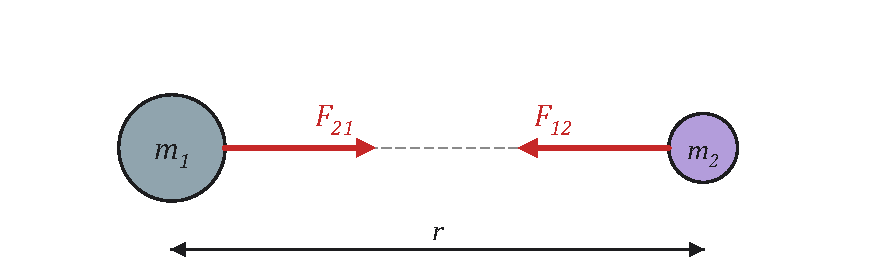
\includegraphics[width=0.6\linewidth]{images/UD4/gravitacion}
    \caption{Las fuerzas con que se atraen dos masas son iguales en módulo, de sentidos opuestos y están sobre la recta que
    une sus centros.}
    \label{fig:grav-fuerza}
\end{figure}

\begin{remark}
    \(G\) es la fuerza con que se atraen dos masas de \qty{1}{\kg} separadas \qty{1}{\m}. Su valor es tan pequeño que la
    atracción entre objetos cotidianos es imperceptible; solo se nota cuando al menos uno de los cuerpos tiene una masa
    enorme. Cavendish lo midió por primera vez en 1798 con una balanza de torsión, lo que permitió «pesar la Tierra».
\end{remark}

\paragraph{Principio de superposición.} Si sobre una masa actúan varias, la fuerza total es la suma vectorial de las
fuerzas que ejerce cada una por separado: \(\vec F = \vec F_1 + \vec F_2 + \vec F_3 + \cdots\) Para calcularla se escogen unos
ejes, se descompone cada fuerza en componentes \(\vec F = F_x\,\vec{i} + F_y\,\vec{j}\) y se suman.

\begin{exercise}
    Tres masas de \qty{2}{\kg}, \qty{5}{\kg} y \qty{6}{\kg} están en los puntos \((0, 0)\), \((0, 4)\) y \((3, 0)\),
    respectivamente (distancias en metros). Calcula la fuerza gravitatoria sobre la masa del origen.
    \begin{solu}
        \textcolor{blue}{La de \qty{5}{\kg} la atrae hacia \(+Y\) y la de \qty{6}{\kg} hacia \(+X\):}
        \[ \vec F_5 = G\,\dfrac{5\cdot 2}{4^2}\,\vec{j} = 4{,}17\cdot 10^{-11}\,\vec{j}\ \unit{\newton} \qquad
           \vec F_6 = G\,\dfrac{6\cdot 2}{3^2}\,\vec{i} = 8{,}89\cdot 10^{-11}\,\vec{i}\ \unit{\newton} \]
        \(\textcolor{red}{\vec F = (8{,}89\,\vec{i} + 4{,}17\,\vec{j})\cdot 10^{-11}\ \unit{\newton}}\);
        \(F = \textcolor{red}{\qty{9.82e-11}{\newton}}\), \textcolor{red}{a \ang{25.1} del eje \(X\)}.
    \end{solu}
\end{exercise}

\begin{exercise}
    En tres vértices de un cuadrado de \qty{1.5}{\m} de lado hay masas de \qty{5}{\kg}. Calcula la fuerza sobre una masa de
    \qty{3}{\kg} situada en el cuarto vértice.
    \begin{solu}
        \textcolor{blue}{Pongamos la masa de \qty{3}{\kg} en el origen y las otras en \((1{,}5;\,0)\), \((0;\,1{,}5)\) y
        \((1{,}5;\,1{,}5)\). Las dos de los lados ejercen \(F_1 = G\,\dfrac{5\cdot 3}{1{,}5^2} = \qty{4.45e-10}{\newton}\) cada una;
        la de la diagonal, a \(1{,}5\sqrt 2\ \unit{\m}\), \(F_2 = G\,\dfrac{15}{4{,}5} = \qty{2.22e-10}{\newton}\), a \ang{45}.}
        \[ F_x = F_y = 4{,}45\cdot 10^{-10} + 2{,}22\cdot 10^{-10}\cos\ang{45} = \qty{6.02e-10}{\newton} \]
        \(\textcolor{red}{\vec F = 6{,}02\cdot 10^{-10}\,(\vec{i} + \vec{j})\ \unit{\newton}}\); \(F = \textcolor{red}{\qty{8.51e-10}{\newton}}\),
        \textcolor{red}{dirigida hacia el vértice opuesto.}
    \end{solu}
\end{exercise}

\subsection{La tercera ley de Kepler a partir de la ley de Newton}\label{subsec:grav-kepler3}

Para un planeta de masa \(m\) en órbita circular de radio \(r\) alrededor del Sol, la fuerza gravitatoria es la fuerza
centrípeta:
\begin{equation*}
    G\,\dfrac{M_S\,m}{r^2} = m\,\dfrac{v^2}{r} \;\Rightarrow\; v^2 = \dfrac{G M_S}{r} \qquad\text{y con } v = \dfrac{2\pi r}{T}:\qquad
    \dfrac{4\pi^2 r^2}{T^2} = \dfrac{G M_S}{r}
\end{equation*}
\begin{centeredequation}
    \boxed{\dfrac{T^2}{r^3} = \dfrac{4\pi^2}{G M}} \label{eq:grav-kepler3-newton}
\end{centeredequation}
La constante de la tercera ley solo depende de la masa del astro central \(M\). Midiendo el período y el radio de la órbita
de un satélite se puede calcular la masa del astro alrededor del que gira.

\section{El campo gravitatorio}\label{sec:grav-campo}

\subsection{El concepto de campo}\label{subsec:grav-concepto-campo}

Un \rojon{campo} es una región del espacio en la que a cada punto le corresponde un valor de una magnitud física. Si la
magnitud es escalar (la temperatura de una habitación), el campo es escalar; si es vectorial (la fuerza sobre una masa),
es vectorial. La idea de campo sustituye a la «acción a distancia»: una masa modifica el espacio que la rodea, y otra masa
colocada en él nota esa modificación.

Un campo vectorial se representa con \azuln{líneas de campo}: líneas tangentes en cada punto al vector del campo, dibujadas
de forma que su densidad sea proporcional a su módulo. Dos líneas de campo nunca se cortan (en el punto de corte el campo
tendría dos valores).

\subsection{Intensidad del campo gravitatorio}\label{subsec:grav-intensidad}

\begin{definition}[Intensidad del campo gravitatorio]
    La \rojon{intensidad del campo gravitatorio} \(\vec g\) en un punto es la fuerza que actuaría sobre la unidad de masa
    colocada en él: \(\vec g = \vec F/m\). Para el campo creado por una masa puntual (o esférica) \(M\) a una distancia \(r\):
    \begin{centeredequation}
        \boxed{\vec g = -\,G\,\dfrac{M}{r^2}\,\vec u_r} \qquad\qquad g = G\,\dfrac{M}{r^2} \label{eq:grav-g}
    \end{centeredequation}
    Se mide en \unit{\newton\per\kg} (equivalente a \unit{\m\per\second\squared}). Está dirigido hacia la masa que crea el campo.
\end{definition}

Conocido el campo, la fuerza sobre cualquier masa \(m\) es \(\vec F = m\,\vec g\). Si hay varias masas, el campo total es
la suma vectorial de los campos de cada una (\azuln{principio de superposición}, figura~\ref{fig:grav-superposicion}).

\begin{figure}[H]
    \centering
    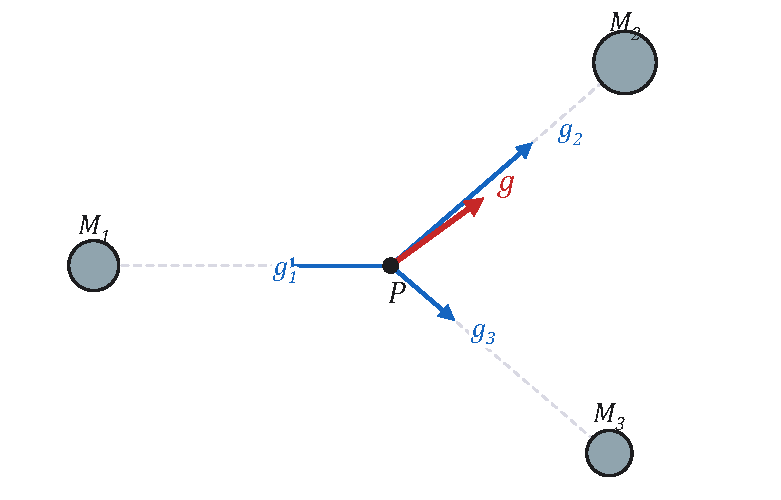
\includegraphics[width=0.5\linewidth]{images/UD4/superposicion}
    \caption{Cada masa crea en \(P\) un campo dirigido hacia ella. El campo total es la suma vectorial.}
    \label{fig:grav-superposicion}
\end{figure}

\begin{exercise}
    Calcula el campo gravitatorio en el punto \(P(4, 3)\) creado por tres masas de \qty{8}{\kg}, \qty{6}{\kg} y \qty{3}{\kg}
    situadas en \((0, 0)\), \((4, 0)\) y \((0, 3)\), respectivamente (distancias en metros).
    \begin{solu}
        \begin{itemize}
            \item \qty{8}{\kg}, a \qty{5}{\m}: \(g_1 = G\,\dfrac{8}{25} = \qty{2.13e-11}{\newton\per\kg}\), dirigido hacia el origen,
            \(\vec u = (-0{,}8;\,-0{,}6)\): \(\vec g_1 = (-1{,}71\,\vec{i} - 1{,}28\,\vec{j})\cdot 10^{-11}\).
            \item \qty{6}{\kg}, a \qty{3}{\m} por debajo: \(\vec g_2 = -G\,\dfrac{6}{9}\,\vec{j} = -4{,}45\cdot 10^{-11}\,\vec{j}\).
            \item \qty{3}{\kg}, a \qty{4}{\m} a la izquierda: \(\vec g_3 = -G\,\dfrac{3}{16}\,\vec{i} = -1{,}25\cdot 10^{-11}\,\vec{i}\).
        \end{itemize}
        \(\textcolor{red}{\vec g = (-2{,}96\,\vec{i} - 5{,}73\,\vec{j})\cdot 10^{-11}\ \unit{\newton\per\kg}}\); \(g = \textcolor{red}{\qty{6.45e-11}{\newton\per\kg}}\).
    \end{solu}
\end{exercise}

\subsection{Líneas del campo gravitatorio}\label{subsec:grav-lineas}

Las líneas del campo de una masa son radiales y se dirigen hacia ella: el campo gravitatorio solo tiene «sumideros», no
«fuentes», porque la gravedad siempre atrae. Cuantas más líneas llegan a una masa, mayor es esta
(figura~\ref{fig:grav-lineas}).

\begin{figure}[H]
    \centering
    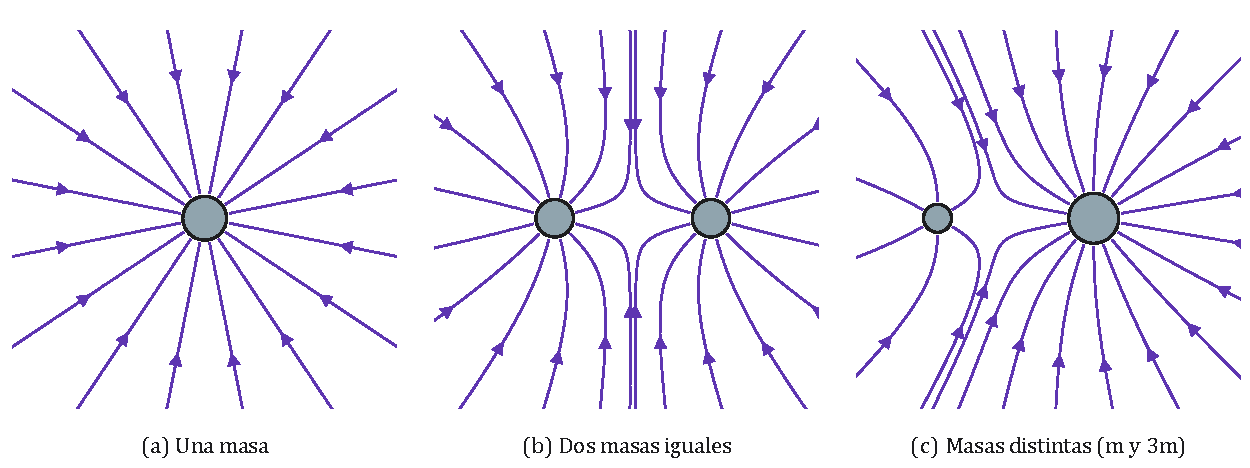
\includegraphics[width=0.95\linewidth]{images/UD4/lineas_campo}
    \caption{Líneas del campo gravitatorio (calculadas con la ley de Newton). En (b), en el punto medio el campo es nulo;
    en (c), a la masa mayor llegan tres veces más líneas.}
    \label{fig:grav-lineas}
\end{figure}

\subsection{El campo gravitatorio terrestre}\label{subsec:grav-terrestre}

Fuera de ella, la Tierra crea el mismo campo que si toda su masa estuviera en su centro. En la superficie:
\begin{centeredequation}
    \boxed{g_0 = G\,\dfrac{M_T}{R_T^2}} = 6{,}67\cdot 10^{-11}\,\dfrac{5{,}98\cdot 10^{24}}{(6{,}37\cdot 10^6)^2} \approx \qty{9.8}{\newton\per\kg} \label{eq:grav-g0}
\end{centeredequation}
De aquí sale una relación muy útil: \(\boxed{G M_T = g_0 R_T^2}\), que permite resolver muchos problemas sin conocer \(G\) ni
\(M_T\).

\paragraph{Variación con la altura.} A una altura \(h\):
\begin{centeredequation}
    g = G\,\dfrac{M_T}{(R_T + h)^2} = g_0\,\dfrac{R_T^2}{(R_T + h)^2} \label{eq:grav-g-altura}
\end{centeredequation}

\paragraph{Variación con la profundidad.} Dentro de la Tierra, a una distancia \(r = R_T - h\) del centro, solo atrae la
masa de la esfera de radio \(r\) (la capa exterior no produce campo neto). Suponiendo la densidad \(\rho\) uniforme, esa masa
es \(m = \rho\,\tfrac{4}{3}\pi r^3\) y \(M_T = \rho\,\tfrac{4}{3}\pi R_T^3\):
\begin{equation*}
    \dfrac{g_h}{g_0} = \dfrac{G m/r^2}{G M_T/R_T^2} = \dfrac{r^3 R_T^2}{R_T^3 r^2} = \dfrac{r}{R_T}
    \qquad\Rightarrow\qquad \boxed{g_h = g_0\,\dfrac{R_T - h}{R_T}}
\end{equation*}
Dentro de la Tierra, \(g\) crece linealmente desde cero en el centro; fuera, disminuye con \(1/r^2\)
(figuras~\ref{fig:grav-profundidad} y \ref{fig:grav-g-r}).

\begin{figure}[H]
    \centering
    \begin{minipage}[b]{0.38\linewidth}
        \centering
        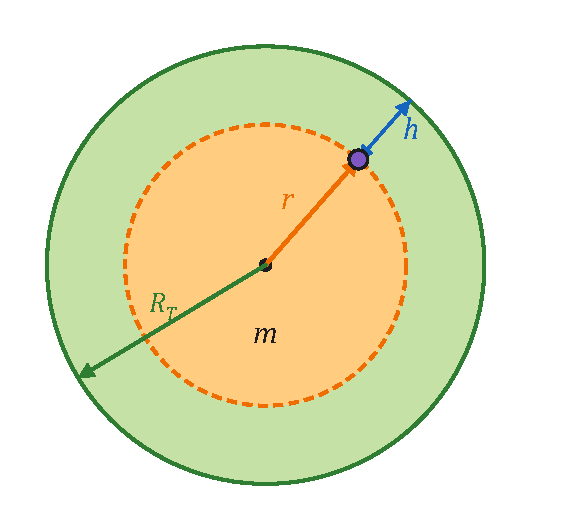
\includegraphics[width=\linewidth]{images/UD4/profundidad}
        \caption{A una profundidad \(h\) solo atrae la esfera interior de radio \(r\).}
        \label{fig:grav-profundidad}
    \end{minipage}\hfill
    \begin{minipage}[b]{0.56\linewidth}
        \centering
        \begin{tikzpicture}
            \begin{axis}[fisica, width=\linewidth, height=5cm, xmin=0, xmax=4.3, ymin=0, ymax=1.25,
                xlabel={\(r\)}, ylabel={\(g\)}, xtick={1,2,3,4}, xticklabels={\(R_T\),\(2R_T\),\(3R_T\),\(4R_T\)},
                ytick={1}, yticklabels={\(g_0\)}]
                \addplot[domain=0:1, very thick, ocre] {x};
                \addplot[domain=1:4.1, very thick, ocre] {1/x^2};
                \draw[dashed, gray] (axis cs:1,0) -- (axis cs:1,1);
            \end{axis}
        \end{tikzpicture}
        \caption{Intensidad del campo terrestre en función de la distancia al centro.}
        \label{fig:grav-g-r}
    \end{minipage}
\end{figure}

\paragraph{Peso.} El \rojon{peso} de un cuerpo es la fuerza con que lo atrae la Tierra: \(P = m\,g\), un vector dirigido
hacia el centro de la Tierra cuyo módulo depende de la altura (y de la latitud). La masa, en cambio, es la misma en
cualquier lugar.

\begin{exercise}
    ¿Cuánto vale el campo gravitatorio creado por un cuerpo de \qty{500}{\kg} a \qty{5}{\m} de su centro?
    \begin{solu}
        \(g = G\,\dfrac{M}{r^2} = 6{,}67\cdot 10^{-11}\cdot\dfrac{500}{25} = \textcolor{red}{\qty{1.33e-9}{\newton\per\kg}}\): \textcolor{blue}{insignificante.}
    \end{solu}
\end{exercise}

\begin{exercise}
    ¿A qué distancia de un cuerpo de masa \(4m\) el campo vale lo mismo que a una distancia \(r\) de un cuerpo de masa \(m\)?
    \begin{solu}
        \(G\,\dfrac{4m}{r'^2} = G\,\dfrac{m}{r^2} \Rightarrow r'^2 = 4r^2 \Rightarrow \textcolor{red}{r' = 2r}\).
    \end{solu}
\end{exercise}

\begin{exercise}
    ¿A qué altura hay que subir para que la intensidad del campo terrestre disminuya un \qty{19}{\percent}? ¿Y para que el
    peso de una persona se reduzca al \qty{64}{\percent}? (\(R_T = \qty{6370}{\km}\)).
    \begin{solu}
        \textcolor{blue}{\(\dfrac{g}{g_0} = \dfrac{R_T^2}{(R_T + h)^2} \Rightarrow R_T + h = R_T\sqrt{g_0/g}\).}

        \(g = 0{,}81\,g_0\): \(R_T + h = \dfrac{R_T}{0{,}9} \Rightarrow h = \dfrac{R_T}{9} = \textcolor{red}{\qty{708}{\km}}\).

        \(P = 0{,}64\,P_0\): \(R_T + h = \dfrac{R_T}{0{,}8} \Rightarrow h = \dfrac{R_T}{4} = \textcolor{red}{\qty{1592}{\km}}\).
    \end{solu}
\end{exercise}

\begin{exercise}
    Júpiter tiene una densidad media de \qty{1.33}{\g\per\cm\cubed} y un radio de \qty{6.99e4}{\km}. Calcula la intensidad del
    campo gravitatorio en su superficie.
    \begin{solu}
        \textcolor{blue}{\(M = \rho\,\tfrac{4}{3}\pi R^3\), así que \(g = G\,\dfrac{M}{R^2} = \tfrac{4}{3}\pi G\rho R\):}
        \[ g = \tfrac{4}{3}\pi\cdot 6{,}67\cdot 10^{-11}\cdot 1330\cdot 6{,}99\cdot 10^7 = \textcolor{red}{\qty{26.0}{\newton\per\kg}} \]
    \end{solu}
\end{exercise}

\section{Energía potencial gravitatoria}\label{sec:grav-energia}

\subsection{La fuerza gravitatoria es conservativa}\label{subsec:grav-conservativa}

Calculemos el trabajo que hace la fuerza gravitatoria de una masa \(M\) sobre otra \(m\) que va de \(A\) a \(B\) por dos
caminos formados por tramos radiales y arcos de circunferencia centrados en \(M\) (figura~\ref{fig:grav-trabajo}). En los
arcos la fuerza es perpendicular al desplazamiento y no trabaja; en los tramos radiales, \(\vec F\) y \(d\vec r\) son
opuestos:
\begin{equation*}
    W_{A\to B} = \int_{r_A}^{r_B} -\,G\,\dfrac{M m}{r^2}\,dr = G M m\left[\dfrac{1}{r}\right]_{r_A}^{r_B} = \dfrac{G M m}{r_B} - \dfrac{G M m}{r_A}
\end{equation*}
Por los dos caminos sale lo mismo, y cualquier camino se puede aproximar por pequeños tramos radiales y arcos. El trabajo
\textbf{no depende de la trayectoria}, solo de las posiciones inicial y final; y en una trayectoria cerrada es nulo. La
fuerza gravitatoria es \rojon{conservativa}, como todas las fuerzas centrales.

\begin{figure}[H]
    \centering
    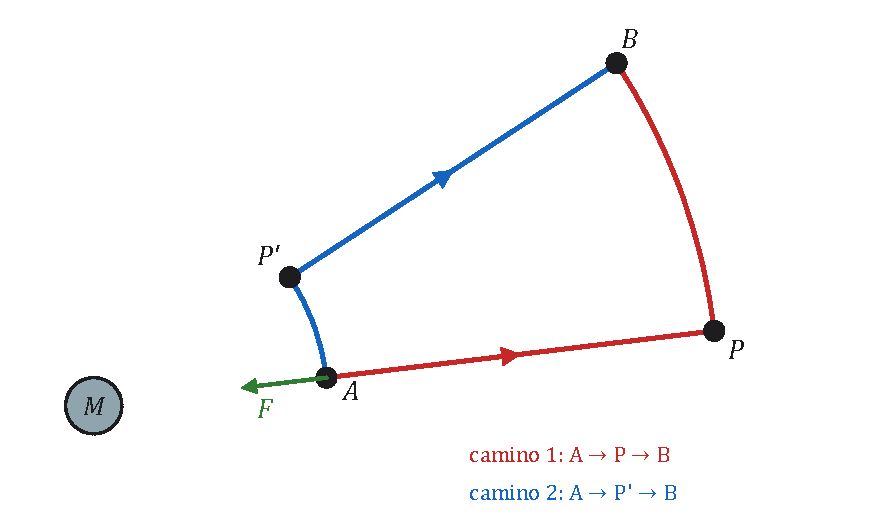
\includegraphics[width=0.55\linewidth]{images/UD4/trabajo_conservativo}
    \caption{El trabajo de la fuerza gravitatoria de \(A\) a \(B\) es el mismo por los dos caminos.}
    \label{fig:grav-trabajo}
\end{figure}

\subsection{Energía potencial}\label{subsec:grav-ep}

Para una fuerza conservativa se puede definir una energía potencial tal que \(W_{A\to B} = -\Delta E_p = E_{p,A} - E_{p,B}\).
Comparando con el trabajo calculado, y tomando \(E_p = 0\) en el infinito:
\begin{centeredequation}
    \boxed{E_p = -\,G\,\dfrac{M m}{r}} \label{eq:grav-ep}
\end{centeredequation}
La energía potencial de dos masas separadas una distancia \(r\) es el trabajo que hace la fuerza gravitatoria cuando se
separan hasta el infinito. Es \textbf{siempre negativa} y aumenta (se hace menos negativa) al alejarse: hay que hacer un
trabajo contra el campo para separarlas. Es una magnitud escalar que se mide en julios. Si hay más de dos masas, la energía
potencial del sistema es la suma de las energías de cada pareja.

\begin{figure}[H]
    \centering
    \begin{tikzpicture}
        \begin{axis}[fisica, width=0.55\linewidth, height=4.6cm, xmin=0, xmax=5.3, ymin=-1.15, ymax=0.25,
            xlabel={\(r\)}, ylabel={\(E_p\)}, xtick=\empty, ytick=\empty, axis x line=middle]
            \addplot[domain=0.9:5, very thick, ocre] {-1/x};
        \end{axis}
    \end{tikzpicture}
    \caption{La energía potencial gravitatoria es negativa y tiende a cero en el infinito.}
    \label{fig:grav-ep}
\end{figure}

\paragraph{Cerca de la superficie: \(E_p = mgh\).} Al subir un cuerpo desde la superficie hasta una altura \(h\):
\begin{equation*}
    \Delta E_p = -\dfrac{G M_T m}{R_T + h} + \dfrac{G M_T m}{R_T} = G M_T m\,\dfrac{h}{R_T(R_T + h)} = m\,g_0\,\dfrac{R_T\,h}{R_T + h}
\end{equation*}
Si \(h \ll R_T\), \(R_T + h \approx R_T\) y queda \(\Delta E_p = m g_0 h\), la expresión que se usa en los cursos anteriores.
Para alturas grandes hay que usar la expresión general.

\begin{exercise}
    Dos partículas de \qty{3}{\kg} y \qty{5}{\kg} están separadas \qty{30}{\cm}. Calcula la energía potencial del sistema, el
    trabajo de la fuerza gravitatoria al separarlas hasta \qty{90}{\cm} y el trabajo para llevar una de ellas al infinito.
    \begin{solu}
        \(E_{p,1} = -G\,\dfrac{3\cdot 5}{0{,}3} = \textcolor{red}{\qty{-3.34e-9}{\joule}}\); \(E_{p,2} = -G\,\dfrac{15}{0{,}9} = \qty{-1.11e-9}{\joule}\).

        \(W = -\Delta E_p = E_{p,1} - E_{p,2} = \textcolor{red}{\qty{-2.22e-9}{\joule}}\);
        \(W_{\to\infty} = E_{p,1} - 0 = \textcolor{red}{\qty{-3.34e-9}{\joule}}\).
        \textcolor{blue}{Son negativos: la gravedad se opone a la separación.}
    \end{solu}
\end{exercise}

\begin{exercise}
    ¿Cuál es la energía potencial de un satélite de \qty{5000}{\kg} que orbita a \qty{600}{\km} de altura?
    (\(M_T = \qty{5.98e24}{\kg}\), \(R_T = \qty{6370}{\km}\)).
    \begin{solu}
        \(E_p = -\dfrac{G M_T m}{R_T + h} = -\dfrac{6{,}67\cdot 10^{-11}\cdot 5{,}98\cdot 10^{24}\cdot 5000}{6{,}97\cdot 10^6} = \textcolor{red}{\qty{-2.86e11}{\joule}}\).
    \end{solu}
\end{exercise}

\begin{exercise}
    Calcula la energía potencial del sistema formado por tres masas de \qty{3}{\kg}, \qty{5}{\kg} y \qty{4}{\kg} situadas en
    \((0, 0)\), \((0, 4)\) y \((3, 0)\) (en metros).
    \begin{solu}
        \textcolor{blue}{Distancias: \(r_{12} = 4\), \(r_{13} = 3\), \(r_{23} = 5\) m.}
        \[ E_p = -G\left(\dfrac{3\cdot 5}{4} + \dfrac{3\cdot 4}{3} + \dfrac{5\cdot 4}{5}\right) = -6{,}67\cdot 10^{-11}\cdot 11{,}75 = \textcolor{red}{\qty{-7.84e-10}{\joule}} \]
    \end{solu}
\end{exercise}

\section{Potencial gravitatorio}\label{sec:grav-potencial}

\begin{definition}[Potencial gravitatorio]
    El \rojon{potencial gravitatorio} \(V\) en un punto es la energía potencial por unidad de masa colocada en él:
    \(V = E_p/m\). Para una masa puntual \(M\):
    \begin{centeredequation}
        \boxed{V = -\,G\,\dfrac{M}{r}} \label{eq:grav-V}
    \end{centeredequation}
    Es un escalar, se mide en \unit{\joule\per\kg} y es nulo en el infinito. El potencial creado por varias masas es la suma
    (escalar) de los potenciales de cada una.
\end{definition}

\paragraph{Diferencia de potencial y trabajo.} Como \(W = -\Delta E_p\) y \(E_p = mV\), el trabajo que hace el campo al
llevar una masa \(m\) de \(A\) a \(B\) es:
\begin{centeredequation}
    \boxed{W_{A\to B} = -\,m\,(V_B - V_A) = m\,(V_A - V_B)} \label{eq:grav-trabajo-V}
\end{centeredequation}
Si \(W > 0\), el desplazamiento es espontáneo (la masa va hacia potenciales menores); si \(W < 0\), hay que aportar energía.

\paragraph{Superficies equipotenciales.} Son los lugares geométricos de los puntos con el mismo potencial. Para una masa
puntual son esferas centradas en ella. Las líneas de campo son siempre \textbf{perpendiculares} a las superficies
equipotenciales, y mover una masa sobre una equipotencial no cuesta trabajo (figura~\ref{fig:grav-equipotenciales}).

\begin{figure}[H]
    \centering
    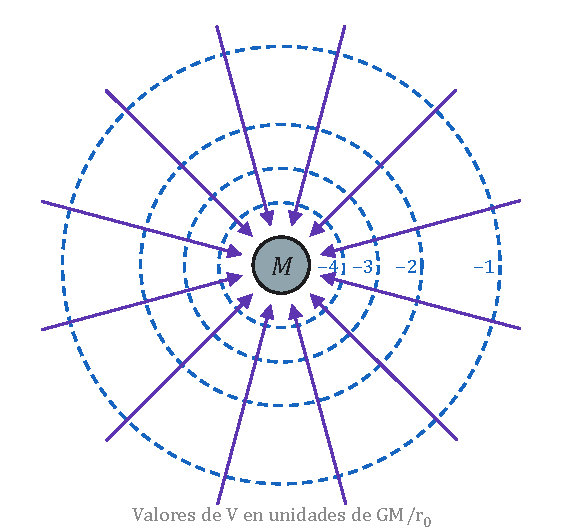
\includegraphics[width=0.42\linewidth]{images/UD4/equipotenciales}
    \caption{Superficies equipotenciales (en discontinuo) y líneas de campo de una masa puntual.}
    \label{fig:grav-equipotenciales}
\end{figure}

\begin{exercise}
    Dos masas de \qty{5}{\kg} están en \((0, 0)\) y \((8, 0)\) (en metros). Calcula el trabajo que hace el campo al llevar una
    masa de \qty{1}{\kg} desde el punto \((4, 3)\) hasta el \((4, 0)\).
    \begin{solu}
        \textcolor{blue}{En \(A(4, 3)\) cada masa está a \qty{5}{\m}; en \(B(4, 0)\), a \qty{4}{\m}.}
        \[ V_A = -2\,G\,\dfrac{5}{5} = \qty{-1.334e-10}{\joule\per\kg} \qquad V_B = -2\,G\,\dfrac{5}{4} = \qty{-1.668e-10}{\joule\per\kg} \]
        \(W = m(V_A - V_B) = \textcolor{red}{\qty{3.34e-11}{\joule}}\) \textcolor{blue}{(positivo: el campo lo hace solo).}
    \end{solu}
\end{exercise}

\section{Movimiento de planetas y satélites}\label{sec:grav-satelites}

\subsection{Velocidad orbital y período}\label{subsec:grav-orbital}

Un satélite de masa \(m\) en órbita circular de radio \(r = R + h\) alrededor de un planeta de masa \(M\) y radio \(R\) está
sometido solo a la atracción gravitatoria, que hace de fuerza centrípeta (figura~\ref{fig:grav-satelite}):
\begin{equation*}
    G\,\dfrac{M m}{r^2} = m\,\dfrac{v^2}{r} \qquad\Rightarrow\qquad \boxed{v = \sqrt{\dfrac{G M}{r}}} \qquad\qquad \boxed{T = \dfrac{2\pi r}{v} = 2\pi\sqrt{\dfrac{r^3}{G M}}}
\end{equation*}
La velocidad orbital no depende de la masa del satélite y es menor cuanto más alta es la órbita.

\begin{figure}[H]
    \centering
    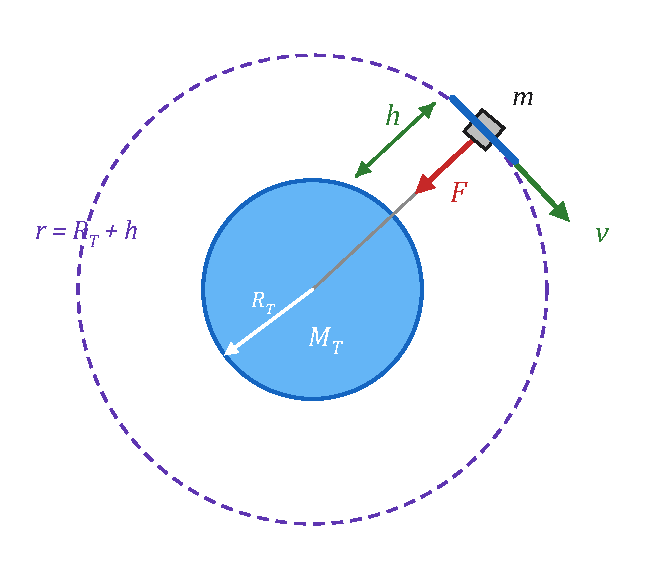
\includegraphics[width=0.45\linewidth]{images/UD4/satelite}
    \caption{Satélite en órbita circular a una altura \(h\).}
    \label{fig:grav-satelite}
\end{figure}

\paragraph{Satélites geoestacionarios.} Si el período de un satélite es igual al de rotación de la Tierra (un día sidéreo,
\qty{86164}{\second}) y gira en el plano del ecuador, en el mismo sentido que la Tierra, está siempre sobre el mismo punto de
la superficie. Se usan para comunicaciones y televisión.

\subsection{Energía de un satélite en órbita}\label{subsec:grav-energia-satelite}

Con \(v^2 = G M/r\):
\begin{equation*}
    E_c = \dfrac{1}{2} m v^2 = \dfrac{G M m}{2r} \qquad\qquad E_p = -\,\dfrac{G M m}{r}
\end{equation*}
\begin{centeredequation}
    \boxed{E_m = E_c + E_p = -\,\dfrac{G M m}{2r}} \qquad\qquad E_c = -E_m = -\tfrac{1}{2}E_p \label{eq:grav-em-orbita}
\end{centeredequation}
La energía mecánica de un satélite en órbita es negativa: está \emph{ligado} al planeta. Si solo actúa la gravedad, la
energía mecánica se conserva: \(\tfrac{1}{2}m v_1^2 - \dfrac{GMm}{r_1} = \tfrac{1}{2}m v_2^2 - \dfrac{GMm}{r_2}\).

\paragraph{Energía para poner un satélite en órbita.} Desde la superficie (despreciando la rotación de la Tierra y el
rozamiento), la energía que hay que comunicar es la diferencia entre la energía mecánica en la órbita y la energía potencial
en la superficie:
\begin{equation*}
    \Delta E = -\,\dfrac{G M m}{2r} - \left(-\,\dfrac{G M m}{R}\right) = G M m\left(\dfrac{1}{R} - \dfrac{1}{2r}\right)
\end{equation*}

\paragraph{Energía para cambiar de órbita.} Para pasar de una órbita de radio \(r_1\) a otra de radio \(r_2\):
\(\Delta E = E_{m,2} - E_{m,1} = \dfrac{G M m}{2}\left(\dfrac{1}{r_1} - \dfrac{1}{r_2}\right)\).

\begin{exercise}
    Un meteorito de \qty{500}{\kg} está en reposo a una altura igual a tres veces el radio terrestre. Si cae sin rozamiento,
    ¿con qué velocidad llega a la superficie? (\(M_T = \qty{5.98e24}{\kg}\), \(R_T = \qty{6370}{\km}\)).
    \begin{solu}
        \textcolor{blue}{Parte de \(r_1 = 4R_T\) con \(v_1 = 0\). Conservación de la energía:}
        \[ -\dfrac{G M_T m}{4R_T} = \dfrac{1}{2}m v^2 - \dfrac{G M_T m}{R_T} \;\Rightarrow\; v = \sqrt{2 G M_T\left(\dfrac{1}{R_T} - \dfrac{1}{4R_T}\right)} = \sqrt{\dfrac{3 G M_T}{2 R_T}} = \textcolor{red}{\qty{9.69e3}{\m\per\second}} \]
        \textcolor{blue}{(No depende de la masa del meteorito.)}
    \end{solu}
\end{exercise}

\begin{exercise}
    Se quiere poner en órbita circular de \qty{7500}{\km} de radio un satélite de \qty{800}{\kg} lanzado desde la superficie
    terrestre. ¿Qué energía hay que comunicarle? Si después se pasa a una órbita de \qty{9000}{\km} de radio, ¿cuánta energía
    hace falta? (\(M_T = \qty{5.98e24}{\kg}\), \(R_T = \qty{6370}{\km}\)).
    \begin{solu}
        \(\Delta E_1 = G M_T m\left(\dfrac{1}{R_T} - \dfrac{1}{2r_1}\right) = 3{,}19\cdot 10^{17}\left(\dfrac{1}{6{,}37\cdot 10^6} - \dfrac{1}{1{,}5\cdot 10^7}\right) = \textcolor{red}{\qty{2.88e10}{\joule}}\).

        \(\Delta E_2 = \dfrac{G M_T m}{2}\left(\dfrac{1}{r_1} - \dfrac{1}{r_2}\right) = \textcolor{red}{\qty{3.55e9}{\joule}}\).
    \end{solu}
\end{exercise}

\subsection{Velocidad de escape}\label{subsec:grav-escape}

\begin{definition}[Velocidad de escape]
    La \rojon{velocidad de escape} es la velocidad mínima que hay que comunicar a un cuerpo en la superficie de un astro
    para que escape de su atracción, es decir, para que llegue al infinito (\(E_p = 0\)) con velocidad nula (\(E_c = 0\)).
\end{definition}
Por la conservación de la energía:
\begin{equation*}
    \dfrac{1}{2}m v_e^2 - \dfrac{G M m}{R} = 0 + 0 \qquad\Rightarrow\qquad \boxed{v_e = \sqrt{\dfrac{2 G M}{R}} = \sqrt{2 g_0 R}}
\end{equation*}
No depende de la masa del cuerpo. Para la Tierra vale unos \qty{11.2}{\km\per\second} y para la Luna, \qty{2.4}{\km\per\second}.
Un cuerpo lanzado con la velocidad de escape tiene energía mecánica nula; si la supera, su energía es positiva y no vuelve.

\begin{remark}
    Según su energía mecánica, un cuerpo en el campo de un astro: si \(E_m < 0\), está ligado y describe una órbita cerrada
    (circular o elíptica); si \(E_m = 0\), escapa justo (trayectoria parabólica); si \(E_m > 0\), escapa con velocidad sobrante
    (trayectoria hiperbólica).
\end{remark}

\section{Resumen de fórmulas}\label{sec:grav-resumen}

\begin{table}[H]
    \centering
    \caption{Fórmulas principales de la interacción gravitatoria}
    \vspace{-5pt}
    \begin{tabular}{@{}lL{10cm}@{}}
        \toprule
        \textbf{Magnitud} & \textbf{Expresión} \\
        \midrule
        Tercera ley de Kepler & \(T^2/r^3 = 4\pi^2/(GM)\) \\[3pt]
        Momento angular & \(\vec L = \vec r\times m\vec v\); \quad fuerza central: \(\vec L\) constante, \(r_p v_p = r_a v_a\) \\[3pt]
        Gravitación universal & \(F = G\,m_1 m_2/r^2\), \quad \(G = \qty{6.67e-11}{\newton\m\squared\per\kg\squared}\) \\[3pt]
        Campo gravitatorio & \(g = GM/r^2\), \quad \(\vec F = m\vec g\), \quad \(G M_T = g_0 R_T^2\) \\[3pt]
        Campo dentro de la Tierra & \(g_h = g_0\,(R_T - h)/R_T\) \\[3pt]
        Energía potencial & \(E_p = -\,GMm/r\) \quad (cerca de la superficie, \(\Delta E_p = mgh\)) \\[3pt]
        Potencial & \(V = -\,GM/r\), \quad \(W_{A\to B} = m(V_A - V_B)\) \\[3pt]
        Satélite en órbita & \(v = \sqrt{GM/r}\), \quad \(T = 2\pi\sqrt{r^3/GM}\), \quad \(E_m = -\,GMm/(2r)\) \\[3pt]
        Velocidad de escape & \(v_e = \sqrt{2GM/R} = \sqrt{2 g_0 R}\) \\
        \bottomrule
    \end{tabular}
    \label{tab:grav-resumen}
\end{table}

\section{Prácticas}\label{sec:grav-practicas}

\subsection{Práctica 1: la tercera ley de Kepler con las lunas de Júpiter}\label{subsec:grav-practica-kepler}

\textbf{Objetivo.} Comprobar la tercera ley de Kepler con los satélites galileanos de Júpiter y calcular la masa del planeta.

\textbf{Material.} Datos de la tabla (o medidas propias hechas con un telescopio pequeño o con un programa planetario
gratuito, siguiendo varias noches la posición de las lunas), hoja de cálculo.

\begin{table}[H]
    \centering
    \caption{Satélites galileanos de Júpiter}
    \vspace{-5pt}
    \begin{tabular}{@{}lcccc@{}}
        \toprule
        \textbf{Satélite} & \textbf{\(r\) (\(10^8\) \unit{\m})} & \textbf{\(T\) (días)} & \textbf{\(r^3\) (\unit{\m\cubed})} & \textbf{\(T^2\) (\unit{\second\squared})} \\
        \midrule
        Ío & \num{4.22} & \num{1.769} & & \\[3pt]
        Europa & \num{6.71} & \num{3.551} & & \\[3pt]
        Ganímedes & \num{10.70} & \num{7.155} & & \\[3pt]
        Calisto & \num{18.83} & \num{16.69} & & \\
        \bottomrule
    \end{tabular}
    \label{tab:grav-practica-kepler}
\end{table}

\textbf{Procedimiento.}
\begin{enumerate}[label=\numberballmDarkTeal]
    \item Pasa los radios a metros y los períodos a segundos y completa la tabla.
    \item Representa \(T^2\) frente a \(r^3\). Comprueba que los puntos están sobre una recta que pasa por el origen.
    \item Calcula la pendiente de la recta, \(k = T^2/r^3\).
\end{enumerate}

\textbf{Cálculos y cuestiones.}
\begin{enumerate}[label=\letraminuscula]
    \item Como \(k = 4\pi^2/(G M_J)\), calcula la masa de Júpiter. (Valor aceptado: \qty{1.90e27}{\kg}.)
    \item ¿Por qué la recta debe pasar por el origen?
    \item Busca los datos de cuatro planetas del Sistema Solar, haz la misma gráfica y calcula la masa del Sol.
\end{enumerate}

\subsection{Práctica 2: medida de \texorpdfstring{\(g\)}{g} y de la masa de la Tierra}\label{subsec:grav-practica-g}

\textbf{Objetivo.} Medir la aceleración de la gravedad y, a partir de ella, estimar la masa y la densidad media de la Tierra.

\textbf{Material.} Péndulo simple (hilo y bola), cronómetro y regla (la práctica 2 de la unidad 1); o bien un teléfono
móvil con una aplicación que registre el acelerómetro.

\textbf{Procedimiento.}
\begin{enumerate}[label=\numberballmDarkTeal]
    \item Mide \(g\) con el péndulo (\(g = 4\pi^2 l/T^2\)) para varias longitudes y halla el valor medio.
    \item Alternativa: deja el móvil quieto sobre la mesa y anota la aceleración que marca el sensor en el eje vertical.
\end{enumerate}

\textbf{Cálculos y cuestiones.}
\begin{enumerate}[label=\letraminuscula]
    \item Con \(G M_T = g_0 R_T^2\) y \(R_T = \qty{6370}{\km}\), calcula la masa de la Tierra.
    \item Calcula su densidad media y compárala con la de las rocas de la superficie (unos \qty{2.7}{\g\per\cm\cubed}).
    ¿Qué te dice sobre el interior de la Tierra?
    \item ¿Cuánto debería cambiar \(g\) al subir al último piso del instituto (unos \qty{15}{\m})? ¿Podrías medir esa diferencia
    con tu montaje?
\end{enumerate}


    \newpage

    %! Unidad 4 — Interacción gravitatoria: ejercicios finales (adaptados de la fuente, con datos cambiados y resueltos)
%! Datos generales: G = 6,67·10^-11 N m^2/kg^2; M_T = 5,98·10^24 kg; R_T = 6370 km; g_0 = 9,8 m/s^2

\section{Ejercicios}\label{sec:grav-ejercicios}

Salvo que se indique otra cosa, usa \(G = \qty{6.67e-11}{\newton\m\squared\per\kg\squared}\), \(M_T = \qty{5.98e24}{\kg}\),
\(R_T = \qty{6370}{\km}\) y \(g_0 = \qty{9.8}{\m\per\second\squared}\).

\subsection{Leyes de Kepler y momento angular}

\begin{exercise}
    Si el momento angular de una partícula respecto de un punto es constante, ¿significa que sobre ella no actúa ninguna
    fuerza? Razónalo.
    \begin{solu}
        \textcolor{red}{No.} \textcolor{blue}{\(\vec L\) es constante si el momento de la fuerza es nulo, \(\vec r\times\vec F = 0\). Eso ocurre si
        no hay fuerza, pero también si la fuerza es paralela a \(\vec r\): es el caso de las fuerzas centrales, como la que el Sol
        ejerce sobre un planeta.}
    \end{solu}
\end{exercise}

\begin{exercise}
    Si la velocidad de una partícula es constante, ¿puede variar su momento angular respecto de un punto? Razónalo.
    \begin{solu}
        \textcolor{red}{No.} \textcolor{blue}{Con \(\vec v\) constante el movimiento es rectilíneo y uniforme, y no hay fuerza neta, así que
        \(d\vec L/dt = \vec r\times\vec F = 0\). Geométricamente, \(L = m v\,d\), donde \(d\) es la distancia del punto a la recta de
        la trayectoria, que no cambia.}
    \end{solu}
\end{exercise}

\begin{exercise}
    Un cometa describe una órbita elíptica con el Sol en un foco. Compara entre el perihelio y el afelio: a) su momento
    angular respecto del Sol; b) su velocidad; c) la fuerza que le hace el Sol; d) su energía potencial.
    \begin{solu}
        \begin{enumerate}[label=\letraminuscula]
            \item \textcolor{red}{Es el mismo}: la fuerza es central.
            \item \textcolor{red}{Mayor en el perihelio}, porque \(r_p v_p = r_a v_a\) y \(r_p < r_a\).
            \item \textcolor{red}{Mayor en el perihelio}: \(F \propto 1/r^2\).
            \item \textcolor{red}{Menor (más negativa) en el perihelio}: \(E_p = -GMm/r\). \textcolor{blue}{Lo que pierde de energía potencial lo gana en cinética.}
        \end{enumerate}
    \end{solu}
\end{exercise}

\begin{exercise}
    Saturno tarda \qty{29.5}{años} en dar una vuelta alrededor del Sol. ¿A qué distancia media del Sol está, si la de la Tierra
    es \qty{1.496e8}{\km}?
    \begin{solu}
        \(r_S = r_T\left(\dfrac{T_S}{T_T}\right)^{2/3} = 1{,}496\cdot 10^8\cdot 29{,}5^{2/3} = \textcolor{red}{\qty{1.43e9}{\km}}\).
    \end{solu}
\end{exercise}

\begin{exercise}
    El radio medio de la órbita de Júpiter es \num{5.2} veces el de la Tierra. ¿Cuánto dura un año en Júpiter?
    \begin{solu}
        \(T_J = T_T\left(\dfrac{r_J}{r_T}\right)^{3/2} = 1\cdot 5{,}2^{1{,}5} = \textcolor{red}{\qty{11.9}{años}}\).
    \end{solu}
\end{exercise}

\subsection{Gravitación universal y campo gravitatorio}

\begin{exercise}
    Si la Tierra redujese su radio a la tercera parte sin cambiar su masa, ¿cuánto valdría el campo gravitatorio en su superficie?
    \begin{solu}
        \(g' = G\,\dfrac{M_T}{(R_T/3)^2} = 9\,g_0 = \textcolor{red}{\qty{88.2}{\newton\per\kg}}\).
    \end{solu}
\end{exercise}

\begin{exercise}
    En la recta que une los centros de la Tierra y la Luna hay un punto donde se anulan las dos fuerzas gravitatorias. ¿A
    qué distancia del centro de la Tierra está, si la distancia Tierra-Luna es \qty{3.84e5}{\km} y la masa de la Tierra es 81
    veces la de la Luna?
    \begin{solu}
        \textcolor{blue}{Sea \(x\) la distancia a la Tierra: \(G\,\dfrac{81 M_L}{x^2} = G\,\dfrac{M_L}{(d - x)^2} \Rightarrow \dfrac{x}{d - x} = 9\).}
        \(x = \dfrac{9d}{10} = \textcolor{red}{\qty{3.46e5}{\km}}\).
    \end{solu}
\end{exercise}

\begin{exercise}
    ¿Cuánto pesa un objeto de \qty{50}{\kg} a \qty{300}{\km} de altura sobre la superficie terrestre?
    \begin{solu}
        \(P = G\,\dfrac{M_T m}{(R_T + h)^2} = 6{,}67\cdot 10^{-11}\,\dfrac{5{,}98\cdot 10^{24}\cdot 50}{(6{,}67\cdot 10^6)^2} = \textcolor{red}{\qty{448}{\newton}}\)
        \textcolor{blue}{(en la superficie pesaría \qty{490}{\newton}).}
    \end{solu}
\end{exercise}

\begin{exercise}
    La intensidad del campo gravitatorio en la superficie de Marte es \qty{3.71}{\newton\per\kg} y su radio, \qty{3.39e6}{\m}.
    Calcula la masa de Marte.
    \begin{solu}
        \(M = \dfrac{g R^2}{G} = \dfrac{3{,}71\cdot(3{,}39\cdot 10^6)^2}{6{,}67\cdot 10^{-11}} = \textcolor{red}{\qty{6.39e23}{\kg}}\).
    \end{solu}
\end{exercise}

\begin{exercise}
    ¿A qué altura pierde un cuerpo el \qty{30}{\percent} de su peso? ¿Y a qué altura su peso se reduce al \qty{30}{\percent}?
    \begin{solu}
        \textcolor{blue}{\(\dfrac{P}{P_0} = \dfrac{R_T^2}{(R_T + h)^2} \Rightarrow h = R_T\left(\sqrt{P_0/P} - 1\right)\).}

        \(P = 0{,}7\,P_0\): \(h = 6370\left(\dfrac{1}{\sqrt{0{,}7}} - 1\right) = \textcolor{red}{\qty{1244}{\km}}\).
        \(P = 0{,}3\,P_0\): \(h = \textcolor{red}{\qty{5260}{\km}}\).
    \end{solu}
\end{exercise}

\begin{exercise}
    El diámetro del Sol es 109 veces el de la Tierra y la gravedad en su superficie es 28 veces la terrestre. ¿Cuántas veces
    mayor es la masa del Sol?
    \begin{solu}
        \(g = \dfrac{GM}{R^2} \Rightarrow \dfrac{M_S}{M_T} = \dfrac{g_S}{g_T}\left(\dfrac{R_S}{R_T}\right)^2 = 28\cdot 109^2 = \textcolor{red}{\num{3.33e5}}\).
    \end{solu}
\end{exercise}

\begin{exercise}
    La masa de la Luna es \(1/81\) de la de la Tierra y su radio, \num{0.27} veces el terrestre. ¿Cuánto pesaría en la Luna una
    persona que en la Tierra pesa \qty{735}{\newton}?
    \begin{solu}
        \(\dfrac{g_L}{g_T} = \dfrac{M_L}{M_T}\left(\dfrac{R_T}{R_L}\right)^2 = \dfrac{1}{81\cdot 0{,}27^2} = 0{,}169 \Rightarrow P_L = \textcolor{red}{\qty{124}{\newton}}\).
    \end{solu}
\end{exercise}

\begin{exercise}
    La gravedad en la Luna es \qty{1.62}{\m\per\second\squared}. ¿Cuánto pesa allí una persona de \qty{75}{\kg}? ¿Cuál es su masa?
    \begin{solu}
        \(P = m g_L = 75\cdot 1{,}62 = \textcolor{red}{\qty{121.5}{\newton}}\); \textcolor{red}{su masa sigue siendo \qty{75}{\kg}}.
    \end{solu}
\end{exercise}

\begin{exercise}
    La masa de Marte es \num{0.107} veces la de la Tierra y su radio, \num{0.532} veces. ¿Cuál sería en Marte el período de un
    péndulo que en la Tierra bate \qty{2}{\second}?
    \begin{solu}
        \(\dfrac{g_M}{g_T} = \dfrac{0{,}107}{0{,}532^2} = 0{,}378\);
        \(T_M = T_T\sqrt{\dfrac{g_T}{g_M}} = \dfrac{2}{\sqrt{0{,}378}} = \textcolor{red}{\qty{3.25}{\second}}\).
    \end{solu}
\end{exercise}

\subsection{Energía y potencial}

\begin{exercise}
    Se lanza verticalmente hacia arriba un cuerpo de \qty{1000}{\kg} con una velocidad de \qty{5000}{\m\per\second}. ¿Qué altura
    alcanza (sin rozamiento)?
    \begin{solu}
        \(\dfrac{1}{2}m v^2 - \dfrac{G M_T m}{R_T} = -\dfrac{G M_T m}{r} \Rightarrow \dfrac{1}{r} = \dfrac{1}{R_T} - \dfrac{v^2}{2 G M_T}\)
        \(\Rightarrow r = \qty{7.96e6}{\m}\); \(h = r - R_T = \textcolor{red}{\qty{1589}{\km}}\).
        \textcolor{blue}{(Con \(h = v^2/2g\) saldrían \qty{1276}{\km}: la aproximación \(g\) constante no vale.)}
    \end{solu}
\end{exercise}

\begin{exercise}
    ¿Con qué velocidad hay que lanzar un cuerpo desde la superficie para que alcance una altura igual a la mitad del radio terrestre?
    \begin{solu}
        \(v = \sqrt{2 G M_T\left(\dfrac{1}{R_T} - \dfrac{1}{1{,}5R_T}\right)} = \sqrt{\dfrac{2 G M_T}{3 R_T}} = \textcolor{red}{\qty{6.46e3}{\m\per\second}}\).
    \end{solu}
\end{exercise}

\begin{exercise}
    Un meteorito de \qty{300}{\kg} está en reposo a una altura de cuatro radios terrestres sobre la superficie. Calcula su
    energía mecánica y la velocidad con que llega al suelo (sin rozamiento).
    \begin{solu}
        \textcolor{blue}{\(r = 5R_T\).} \(E_m = E_p = -\dfrac{G M_T m}{5 R_T} = \textcolor{red}{\qty{-3.76e9}{\joule}}\).

        \(v = \sqrt{2 G M_T\left(\dfrac{1}{R_T} - \dfrac{1}{5R_T}\right)} = \textcolor{red}{\qty{1.00e4}{\m\per\second}}\).
    \end{solu}
\end{exercise}

\begin{exercise}
    Calcula el trabajo necesario para llevar un satélite de \qty{800}{\kg} desde una órbita circular de radio \(2R_T\) hasta otra
    de radio \(3R_T\).
    \begin{solu}
        \(\Delta E = \dfrac{G M_T m}{2}\left(\dfrac{1}{2R_T} - \dfrac{1}{3R_T}\right) = \dfrac{G M_T m}{12 R_T} = \dfrac{g_0 R_T m}{12} = \textcolor{red}{\qty{4.16e9}{\joule}}\).
    \end{solu}
\end{exercise}

\subsection{Satélites}

\begin{exercise}
    Suponiendo que la Tierra gira alrededor del Sol en una órbita circular de \qty{1.496e11}{\m} en \qty{365.25}{días}, calcula
    la masa del Sol.
    \begin{solu}
        \(M_S = \dfrac{4\pi^2 r^3}{G T^2} = \dfrac{4\pi^2(1{,}496\cdot 10^{11})^3}{6{,}67\cdot 10^{-11}\,(3{,}156\cdot 10^7)^2} = \textcolor{red}{\qty{1.99e30}{\kg}}\).
    \end{solu}
\end{exercise}

\begin{exercise}
    Calisto, una luna de Júpiter, tiene un período de \qty{16.69}{días} y gira a \qty{1.883e6}{\km} del centro del planeta.
    Calcula la masa de Júpiter.
    \begin{solu}
        \(M_J = \dfrac{4\pi^2 r^3}{G T^2} = \dfrac{4\pi^2(1{,}883\cdot 10^9)^3}{6{,}67\cdot 10^{-11}(1{,}442\cdot 10^6)^2} = \textcolor{red}{\qty{1.90e27}{\kg}}\).
    \end{solu}
\end{exercise}

\begin{exercise}
    Un satélite gira a \qty{600}{\km} de altura con un período de \qty{1.61}{h}. Calcula la masa de la Tierra.
    \begin{solu}
        \(M_T = \dfrac{4\pi^2 (R_T + h)^3}{G T^2} = \dfrac{4\pi^2(6{,}97\cdot 10^6)^3}{6{,}67\cdot 10^{-11}\cdot 5796^2} = \textcolor{red}{\qty{5.97e24}{\kg}}\).
    \end{solu}
\end{exercise}

\begin{exercise}
    Venus gira a \qty{1.082e8}{\km} del Sol y Marte a \qty{2.279e8}{\km}. Suponiendo órbitas circulares, calcula sus velocidades
    orbitales (\(M_S = \qty{1.99e30}{\kg}\)).
    \begin{solu}
        \(v_V = \sqrt{\dfrac{G M_S}{r_V}} = \textcolor{red}{\qty{35.0}{\km\per\second}}\); \(v_M = \textcolor{red}{\qty{24.1}{\km\per\second}}\).
        \textcolor{blue}{El planeta más lejano va más despacio.}
    \end{solu}
\end{exercise}

\begin{exercise}
    Un satélite da una vuelta a la Tierra cada \qty{2}{h}. ¿Cuál es el radio de su órbita y a qué altura está?
    \begin{solu}
        \(r = \sqrt[3]{\dfrac{G M_T T^2}{4\pi^2}} = \sqrt[3]{\dfrac{6{,}67\cdot 10^{-11}\cdot 5{,}98\cdot 10^{24}\cdot 7200^2}{4\pi^2}} = \textcolor{red}{\qty{8.06e6}{\m}}\);
        \(h = \textcolor{red}{\qty{1691}{\km}}\).
    \end{solu}
\end{exercise}

\begin{exercise}
    Un satélite describe una órbita circular a \qty{7.5}{\km\per\second}. ¿A qué altura está y cuál es su período?
    \begin{solu}
        \(r = \dfrac{G M_T}{v^2} = \qty{7.09e6}{\m} \Rightarrow h = \textcolor{red}{\qty{721}{\km}}\);
        \(T = \dfrac{2\pi r}{v} = \textcolor{red}{\qty{1.65}{h}}\).
    \end{solu}
\end{exercise}

\begin{exercise}
    Un satélite meteorológico pasa sobre el mismo punto cuatro veces al día (su período es de \qty{6}{h}). ¿Cuál es el radio de
    su órbita?
    \begin{solu}
        \(r = \sqrt[3]{\dfrac{G M_T T^2}{4\pi^2}} = \textcolor{red}{\qty{1.68e7}{\m}}\) \textcolor{blue}{(unos \qty{10400}{\km} de altura).}
    \end{solu}
\end{exercise}

\begin{exercise}
    Calcula el período de un satélite que gira a \qty{20000}{\km} de altura.
    \begin{solu}
        \(T = 2\pi\sqrt{\dfrac{(R_T + h)^3}{G M_T}} = 2\pi\sqrt{\dfrac{(2{,}637\cdot 10^7)^3}{3{,}99\cdot 10^{14}}} = \textcolor{red}{\qty{11.8}{h}}\)
        \textcolor{blue}{(es la órbita de los satélites GPS).}
    \end{solu}
\end{exercise}

\begin{exercise}
    Sobre los satélites geoestacionarios:
    \begin{enumerate}[label=\letraminuscula]
        \item ¿A qué altura orbitan?
        \item ¿Cuál es el momento angular de uno de \qty{300}{\kg} respecto del centro de la Tierra?
        \item ¿Qué energía hay que comunicarle en la superficie para ponerlo en órbita?
    \end{enumerate}
    \begin{solu}
        \textcolor{blue}{\(T = \qty{86164}{\second}\).}
        \begin{enumerate}[label=\letraminuscula]
            \item \(r = \sqrt[3]{\dfrac{G M_T T^2}{4\pi^2}} = \qty{4.22e7}{\m} \Rightarrow h = \textcolor{red}{\qty{35800}{\km}}\).
            \item \(v = \dfrac{2\pi r}{T} = \qty{3075}{\m\per\second}\); \(L = m r v = \textcolor{red}{\qty{3.89e13}{\kg\m\squared\per\second}}\).
            \item \(\Delta E = G M_T m\left(\dfrac{1}{R_T} - \dfrac{1}{2r}\right) = \textcolor{red}{\qty{1.74e10}{\joule}}\).
        \end{enumerate}
    \end{solu}
\end{exercise}

\begin{exercise}
    Un satélite de comunicaciones de \qty{600}{\kg} se libera en una órbita circular a \qty{400}{\km} de altura y un motor lo
    lleva después a la órbita geoestacionaria. ¿Cuánta energía ha aportado el motor?
    \begin{solu}
        \(\Delta E = \dfrac{G M_T m}{2}\left(\dfrac{1}{r_1} - \dfrac{1}{r_2}\right) = \dfrac{2{,}39\cdot 10^{17}}{2}\left(\dfrac{1}{6{,}77\cdot 10^6} - \dfrac{1}{4{,}22\cdot 10^7}\right) = \textcolor{red}{\qty{1.48e10}{\joule}}\).
    \end{solu}
\end{exercise}

\begin{exercise}
    Un satélite de \qty{200}{\kg} describe una órbita circular a \qty{7.3}{\km\per\second}. Calcula: a) su energía potencial;
    b) su energía mecánica; c) la energía que hubo que comunicarle para ponerlo en órbita; d) la energía necesaria para pasarlo
    a una órbita de radio doble.
    \begin{solu}
        \textcolor{blue}{\(r = G M_T/v^2 = \qty{7.48e6}{\m}\) (a \qty{1115}{\km} de altura).}
        \begin{enumerate}[label=\letraminuscula]
            \item \(E_p = -\dfrac{G M_T m}{r} = -m v^2 = \textcolor{red}{\qty{-1.07e10}{\joule}}\).
            \item \(E_m = \dfrac{E_p}{2} = \textcolor{red}{\qty{-5.33e9}{\joule}}\).
            \item \(\Delta E = E_m - \left(-\dfrac{G M_T m}{R_T}\right) = \textcolor{red}{\qty{7.19e9}{\joule}}\).
            \item \textcolor{blue}{Con radio doble, \(E'_m = E_m/2\):} \(\Delta E = \textcolor{red}{\qty{2.66e9}{\joule}}\).
        \end{enumerate}
    \end{solu}
\end{exercise}

\begin{exercise}
    Venus (\(M = \qty{4.87e24}{\kg}\)) gira alrededor del Sol (\(M_S = \qty{1.99e30}{\kg}\)) en una órbita circular de
    \qty{1.082e8}{\km}. La gravedad en su superficie es \qty{8.87}{\m\per\second\squared}.
    \begin{enumerate}[label=\letraminuscula]
        \item Calcula el diámetro de Venus.
        \item Calcula su velocidad orbital y la duración de su año en días.
        \item ¿Qué velocidad necesitaría Venus para escapar de la atracción del Sol desde su órbita?
    \end{enumerate}
    \begin{solu}
        \begin{enumerate}[label=\letraminuscula]
            \item \(R = \sqrt{\dfrac{G M}{g}} = \qty{6.05e6}{\m} \Rightarrow D = \textcolor{red}{\qty{12100}{\km}}\).
            \item \(v = \sqrt{\dfrac{G M_S}{r}} = \textcolor{red}{\qty{35.0}{\km\per\second}}\); \(T = \dfrac{2\pi r}{v} = \textcolor{red}{\qty{225}{días}}\).
            \item \(v_e = \sqrt{\dfrac{2 G M_S}{r}} = \sqrt 2\,v = \textcolor{red}{\qty{49.5}{\km\per\second}}\).
        \end{enumerate}
    \end{solu}
\end{exercise}

\begin{exercise}
    Una misión quiere colocar un vehículo de \qty{600}{\kg} en una órbita circular de \qty{3800}{\km} de radio alrededor de Marte
    (\(M = \qty{6.42e23}{\kg}\), \(R = \qty{3397}{\km}\)). Calcula: a) su energía cinética y su período; b) su energía potencial y
    su energía mecánica; c) la energía para pasarlo a una órbita a \qty{500}{\km} de altura.
    \begin{solu}
        \begin{enumerate}[label=\letraminuscula]
            \item \(E_c = \dfrac{G M m}{2r} = \textcolor{red}{\qty{3.38e9}{\joule}}\); \(T = 2\pi\sqrt{\dfrac{r^3}{GM}} = \textcolor{red}{\qty{1.98}{h}}\).
            \item \(E_p = -2E_c = \textcolor{red}{\qty{-6.76e9}{\joule}}\); \(E_m = -E_c = \textcolor{red}{\qty{-3.38e9}{\joule}}\).
            \item \textcolor{blue}{\(r_2 = \qty{3.897e6}{\m}\):} \(\Delta E = \dfrac{G M m}{2}\left(\dfrac{1}{r_1} - \dfrac{1}{r_2}\right) = \textcolor{red}{\qty{8.4e7}{\joule}}\).
        \end{enumerate}
    \end{solu}
\end{exercise}


%----------------------------------------------------------------------------------------
%	PARTE: INTERACCIÓN ELECTROMAGNÉTICA
%----------------------------------------------------------------------------------------

    \part{Interacción electromagnética}

    \chapterimage{images/portada_cabeceras/cabecera_UD5}
    \chapter{Campo eléctrico}

    %! Unidad 5 — Campo eléctrico (teoría, actividades resueltas y prácticas)
%! Fuente: Fuentes/Tema_5.pdf (reescrito; datos de las actividades cambiados y recalculados)

\section*{Para empezar: el ámbar y el rayo}
\addcontentsline{toc}{section}{Para empezar: el ámbar y el rayo}

Hace más de 2500 años, Tales de Mileto observó que un trozo de ámbar frotado con lana atraía pequeñas plumas. La palabra
griega para el ámbar, \emph{élektron}, dio nombre a la electricidad. Durante siglos fue una curiosidad de salón, hasta que en
1752 Benjamin Franklin hizo volar una cometa en plena tormenta y demostró que el rayo es una enorme chispa eléctrica. Hoy
sabemos que la fuerza eléctrica es la que mantiene unidos los átomos y las moléculas: es la responsable de casi todo lo que
vemos y tocamos. En esta unidad estudiaremos las cargas en reposo con las mismas herramientas que usamos para la gravedad
(fuerza, campo, energía potencial y potencial) y veremos en qué se parecen y en qué se diferencian las dos interacciones.

\section{La carga eléctrica}\label{sec:ele-carga}

La materia está formada por átomos con un núcleo de \textbf{protones} (con carga positiva) y neutrones, rodeado de
\textbf{electrones} (con carga negativa). Fue Franklin quien llamó \emph{positiva} y \emph{negativa} a los dos tipos de carga.
Un cuerpo es neutro si tiene tantos protones como electrones; está cargado negativamente si tiene electrones de más, y
positivamente si le faltan. Entre los cuerpos solo se transfieren electrones, nunca protones.

Propiedades de la carga eléctrica:
\begin{itemize}
    \item Hay dos tipos: las cargas del mismo signo se repelen y las de signo contrario se atraen.
    \item \textbf{Se conserva}: en un sistema aislado la carga total no cambia; solo pasa de unos cuerpos a otros.
    \item \textbf{Está cuantizada}: cualquier carga es un múltiplo entero de la carga del electrón,
    \(e = \qty{1.6e-19}{\coulomb}\).
\end{itemize}
La unidad de carga en el SI es el \azuln{culombio} (\unit{\coulomb}), la carga que atraviesa en un segundo la sección de un
conductor por el que circula una corriente de un amperio. Es una carga muy grande, así que se usan sus submúltiplos: el
microculombio (\(\qty{1}{\micro\coulomb} = \qty{e-6}{\coulomb}\)) y el nanoculombio (\(\qty{1}{\nano\coulomb} = \qty{e-9}{\coulomb}\)).

Según cómo se mueven las cargas en su interior, los materiales son \azuln{conductores} (metales, grafito, disoluciones de
electrolitos, el cuerpo humano), en los que algunos electrones se mueven con libertad, o \azuln{aislantes} o dieléctricos
(vidrio, plástico, porcelana, ámbar), en los que no.

\subsection{Formas de electrización}\label{subsec:ele-electrizacion}

\begin{itemize}
    \item \textbf{Por frotamiento}. Al frotar dos materiales distintos, los electrones pasan de uno a otro: al frotar un
    plástico con lana, el plástico gana electrones (queda negativo) y la lana los pierde (queda positiva).
    \item \textbf{Por contacto}. Al tocar un cuerpo neutro con otro cargado, parte de la carga pasa al neutro y los dos quedan
    con carga del mismo signo (y se repelen).
    \item \textbf{Por inducción}. Al acercar un cuerpo cargado a un conductor, sin tocarlo, sus electrones se redistribuyen:
    si la varilla es positiva, los electrones se acumulan en el lado más próximo. Si se conecta el conductor a tierra, suben
    electrones desde ella; si se corta la conexión antes de retirar la varilla, el conductor queda cargado negativamente.
\end{itemize}

\begin{figure}[H]
    \centering
    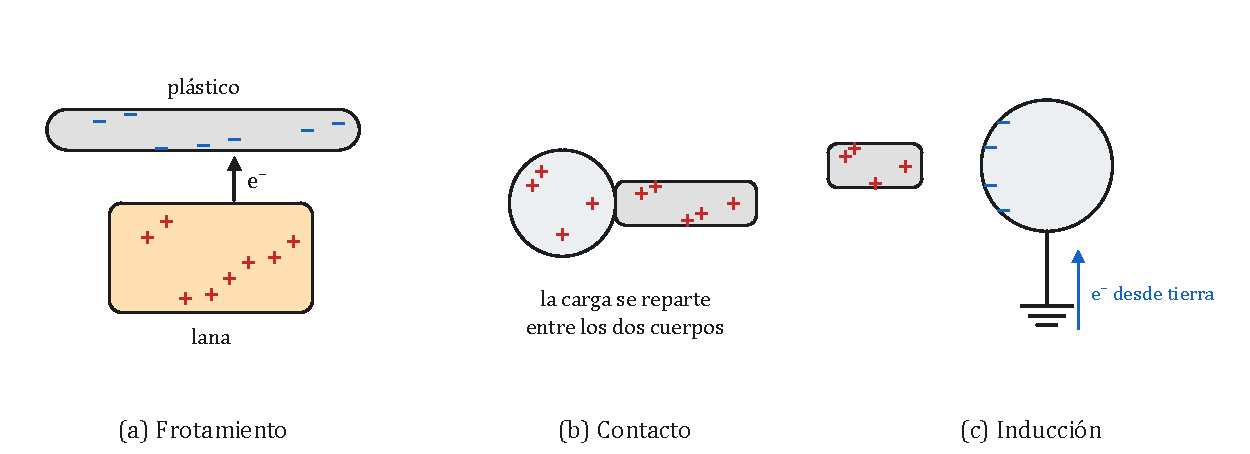
\includegraphics[width=0.95\linewidth]{images/UD5/electrizacion}
    \caption{Las tres formas de electrizar un cuerpo. En todas ellas solo se mueven electrones.}
    \label{fig:ele-electrizacion}
\end{figure}

\section{Ley de Coulomb}\label{sec:ele-coulomb}

En 1785 Charles-Augustin de Coulomb midió con una balanza de torsión la fuerza entre dos esferas cargadas.

\begin{definition}[Ley de Coulomb]
    La fuerza con que se atraen (si tienen signo contrario) o se repelen (si tienen el mismo signo) dos cargas puntuales es
    directamente proporcional al producto de las cargas e inversamente proporcional al cuadrado de la distancia que las separa:
    \begin{centeredequation}
        \boxed{\vec F = k\,\dfrac{Q\,q}{r^2}\,\vec u_r} \qquad\qquad F = k\,\dfrac{|Q|\,|q|}{r^2} \label{eq:ele-coulomb}
    \end{centeredequation}
    donde \(\vec u_r\) es un vector unitario que va de la carga que ejerce la fuerza a la que la sufre.
\end{definition}

Con los signos de las cargas incluidos, si \(Qq > 0\) la fuerza tiene el sentido de \(\vec u_r\) (repulsión) y si \(Qq < 0\),
el contrario (atracción) (figura~\ref{fig:ele-coulomb}).

\begin{figure}[H]
    \centering
    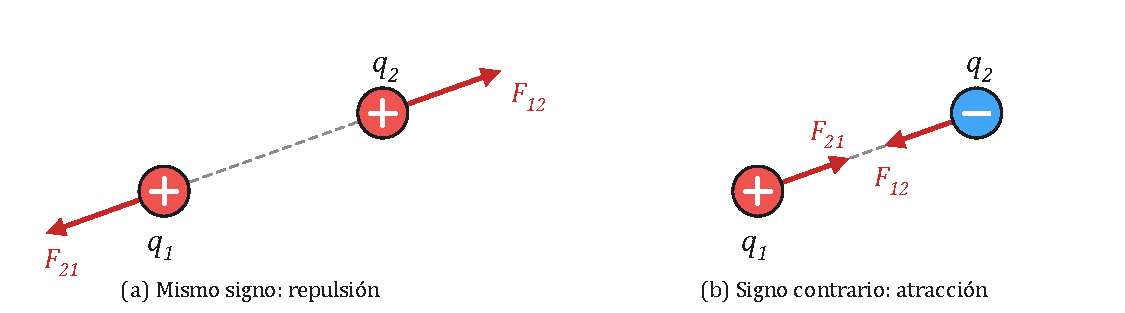
\includegraphics[width=0.8\linewidth]{images/UD5/coulomb}
    \caption{Las fuerzas entre dos cargas son iguales en módulo y de sentidos opuestos (tercera ley de Newton).}
    \label{fig:ele-coulomb}
\end{figure}

La constante \(k\) depende del medio. Se escribe \(k = \dfrac{1}{4\pi\varepsilon}\), donde \(\varepsilon\) es la
\azuln{permitividad} del medio. En el vacío:
\begin{centeredequation}
    \varepsilon_0 = \qty{8.85e-12}{\coulomb\squared\per\newton\per\m\squared} \qquad\qquad k = \dfrac{1}{4\pi\varepsilon_0} = \qty{8.99e9}{\newton\m\squared\per\coulomb\squared} \approx \qty{9e9}{\newton\m\squared\per\coulomb\squared}
\end{centeredequation}
En cualquier otro medio la permitividad es mayor y la fuerza, menor: el agua, por ejemplo, reduce la fuerza unas 80 veces
(por eso disuelve tan bien los compuestos iónicos).

\begin{remark}
    \textbf{Comparación con la gravedad.} Las dos leyes tienen la misma forma (inversamente proporcionales a \(r^2\)), pero:
    \begin{itemize}
        \item la fuerza gravitatoria siempre es atractiva; la eléctrica puede ser atractiva o repulsiva;
        \item \(G\) es universal; \(k\) depende del medio;
        \item la fuerza eléctrica es muchísimo más intensa: entre un protón y un electrón es unas \(10^{39}\) veces mayor que la
        gravitatoria. Si a gran escala domina la gravedad es porque los cuerpos grandes son prácticamente neutros.
    \end{itemize}
\end{remark}

\begin{exercise}
    ¿A qué distancia hay que poner dos cargas de \qty{2}{\micro\coulomb} para que se repelan con una fuerza de \qty{2}{\newton}?
    \begin{solu}
        \(r = \sqrt{\dfrac{k\,q^2}{F}} = \sqrt{\dfrac{9\cdot 10^9\cdot(2\cdot 10^{-6})^2}{2}} = \textcolor{red}{\qty{0.134}{\m} = \qty{13.4}{\cm}}\).
    \end{solu}
\end{exercise}

\begin{exercise}
    ¿Qué significado físico tiene la constante \(k\) de la ley de Coulomb?
    \begin{solu}
        \textcolor{blue}{Despejando, \(k = F r^2/(Qq)\).} \textcolor{red}{Es la fuerza con que se repelen dos cargas de
        \qty{1}{\coulomb} separadas \qty{1}{\m} en ese medio}: \textcolor{blue}{en el vacío, \qty{9e9}{\newton}, una fuerza enorme.}
    \end{solu}
\end{exercise}

\begin{exercise}
    Una partícula de \qty{50}{\g} con una carga de \qty{1}{\micro\coulomb} se mantiene en equilibrio \qty{30}{\cm} por encima
    de otra partícula fija, en su misma vertical. ¿Qué carga tiene la segunda partícula?
    \begin{solu}
        \textcolor{blue}{La fuerza eléctrica (repulsiva, hacia arriba) equilibra el peso: \(k\,\dfrac{q_1 q_2}{r^2} = mg\).}
        \[ q_2 = \dfrac{m g r^2}{k q_1} = \dfrac{0{,}05\cdot 9{,}8\cdot 0{,}3^2}{9\cdot 10^9\cdot 10^{-6}} = \textcolor{red}{\qty{4.9e-6}{\coulomb}} \]
        \textcolor{red}{Positiva}, \textcolor{blue}{para que haya repulsión.}
    \end{solu}
\end{exercise}

\paragraph{Principio de superposición.} Si sobre una carga actúan varias, la fuerza total es la suma vectorial de las fuerzas
que ejerce cada una: \(\vec F = \vec F_1 + \vec F_2 + \cdots\) Para calcularla: se ponen los ejes con el origen en la carga, se
calcula el módulo de cada fuerza, se dibuja su sentido (atracción o repulsión), se descompone en componentes y se suma.

\begin{exercise}
    Tres cargas de \qty{-3}{\micro\coulomb}, \qty{4}{\micro\coulomb} y \qty{2}{\micro\coulomb} están en los puntos \((3, 0)\),
    \((0, 4)\) y \((0, 0)\), con las coordenadas en centímetros. Calcula la fuerza sobre la tercera carga.
    \begin{solu}
        \textcolor{blue}{La de \qty{-3}{\micro\coulomb} atrae a la del origen hacia \(+X\); la de \qty{4}{\micro\coulomb} la repele hacia \(-Y\):}
        \[ F_1 = 9\cdot 10^9\,\dfrac{3\cdot 10^{-6}\cdot 2\cdot 10^{-6}}{0{,}03^2} = \qty{60}{\newton} \qquad F_2 = 9\cdot 10^9\,\dfrac{4\cdot 10^{-6}\cdot 2\cdot 10^{-6}}{0{,}04^2} = \qty{45}{\newton} \]
        \(\textcolor{red}{\vec F = 60\,\vec{i} - 45\,\vec{j}\ \unit{\newton}}\); \(F = \textcolor{red}{\qty{75}{\newton}}\).
    \end{solu}
\end{exercise}

\section{El campo eléctrico}\label{sec:ele-campo}

Una carga modifica el espacio que la rodea: crea un \rojon{campo eléctrico}. Otra carga colocada en él experimenta una fuerza.

\begin{definition}[Intensidad del campo eléctrico]
    La \rojon{intensidad del campo eléctrico} en un punto es la fuerza que actuaría sobre la unidad de carga positiva colocada
    en él: \(\vec E = \vec F/q\). Para el campo creado por una carga puntual \(Q\) a una distancia \(r\):
    \begin{centeredequation}
        \boxed{\vec E = k\,\dfrac{Q}{r^2}\,\vec u_r} \qquad\qquad E = k\,\dfrac{|Q|}{r^2} \label{eq:ele-E}
    \end{centeredequation}
    Se mide en \unit{\newton\per\coulomb}. Si \(Q > 0\), el campo se aleja de la carga; si \(Q < 0\), se dirige hacia ella.
\end{definition}

Conocido el campo, la fuerza sobre una carga \(q\) es \(\vec F = q\,\vec E\): sobre una carga positiva tiene el sentido del
campo, y sobre una negativa, el contrario. El campo creado por varias cargas es la suma vectorial de los campos de cada una
(\azuln{principio de superposición}).

\begin{exercise}
    Dos cargas de \qty{2e-8}{\coulomb} están en los puntos \((3, 0)\) y \((-3, 0)\) (en centímetros).
    \begin{enumerate}[label=\letraminuscula]
        \item Calcula el campo en el punto \((-6, 0)\) si las dos son positivas.
        \item Calcula el campo en el punto \((0, 3)\) si la de \((3, 0)\) es positiva y la de \((-3, 0)\), negativa.
    \end{enumerate}
    \begin{solu}
        \begin{enumerate}[label=\letraminuscula]
            \item \textcolor{blue}{Las dos están a la derecha del punto, a \qty{9}{\cm} y \qty{3}{\cm}; sus campos apuntan hacia \(-X\):}
            \(E_1 = 9\cdot 10^9\,\dfrac{2\cdot 10^{-8}}{0{,}09^2} = \qty{2.22e4}{\newton\per\coulomb}\);
            \(E_2 = \dfrac{9\cdot 10^9\cdot 2\cdot 10^{-8}}{0{,}03^2} = \qty{2e5}{\newton\per\coulomb}\).
            \(\textcolor{red}{\vec E = -2{,}22\cdot 10^5\,\vec{i}\ \unit{\newton\per\coulomb}}\).
            \item \textcolor{blue}{Las dos están a \(\sqrt{18}\ \unit{\cm}\): cada campo vale \(E = \qty{1e5}{\newton\per\coulomb}\). El de la
            positiva se aleja de ella, dirección \((-1, 1)/\sqrt 2\); el de la negativa va hacia ella, \((-1, -1)/\sqrt 2\). Las
            componentes \(y\) se anulan:}
            \(\textcolor{red}{\vec E = -2E\cos\ang{45}\,\vec{i} = -1{,}41\cdot 10^5\,\vec{i}\ \unit{\newton\per\coulomb}}\).
        \end{enumerate}
    \end{solu}
\end{exercise}

\subsection{Líneas del campo eléctrico}\label{subsec:ele-lineas}

Las líneas del campo eléctrico son tangentes en cada punto al vector \(\vec E\). \textbf{Salen de las cargas positivas}
(fuentes) y \textbf{llegan a las negativas} (sumideros); su número es proporcional a la carga y nunca se cortan
(figura~\ref{fig:ele-lineas}). Indican la trayectoria que seguiría una carga positiva muy pequeña abandonada en reposo solo
al principio de su movimiento, porque después la velocidad ya no tiene por qué seguir la línea.

\begin{figure}[H]
    \centering
    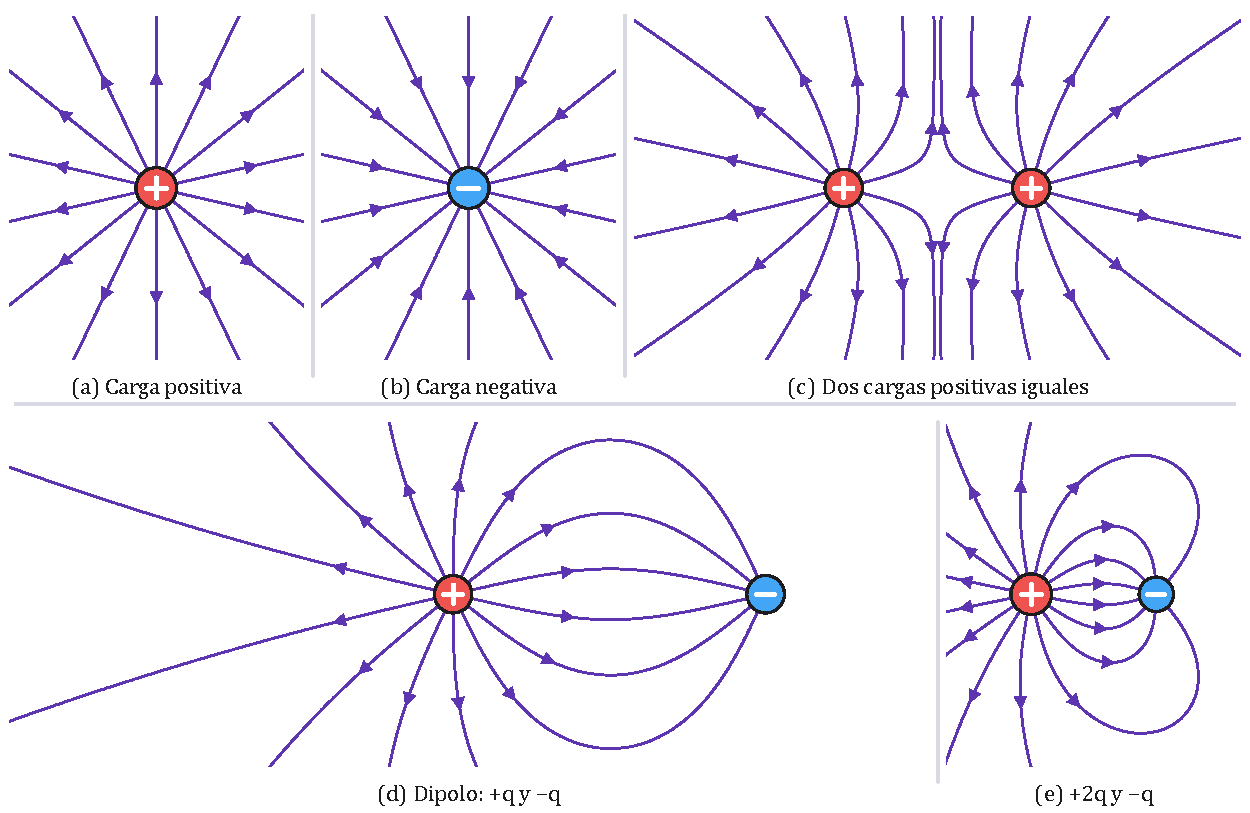
\includegraphics[width=0.95\linewidth]{images/UD5/lineas_campo}
    \caption{Líneas del campo eléctrico calculadas con la ley de Coulomb. Entre dos cargas iguales hay un punto en el que el
    campo es nulo; en (e), de la carga \(+2q\) salen el doble de líneas de las que llegan a \(-q\), y la mitad se van al infinito.}
    \label{fig:ele-lineas}
\end{figure}

\section{Energía potencial eléctrica}\label{sec:ele-energia}

La fuerza eléctrica es central y, como la gravitatoria, \textbf{conservativa}. Repitiendo el cálculo de la unidad anterior, el
trabajo que hace el campo de una carga \(Q\) sobre otra \(q\) que va de \(A\) a \(B\) es:
\begin{equation*}
    W_{A\to B} = \int_{r_A}^{r_B} k\,\dfrac{Q q}{r^2}\,dr = k\,\dfrac{Q q}{r_A} - k\,\dfrac{Q q}{r_B} = E_{p,A} - E_{p,B}
\end{equation*}
Tomando \(E_p = 0\) en el infinito, la \rojon{energía potencial eléctrica} de dos cargas separadas una distancia \(r\) es:
\begin{centeredequation}
    \boxed{E_p = k\,\dfrac{Q\,q}{r}} \label{eq:ele-ep}
\end{centeredequation}
Ahora los signos de las cargas importan: \(E_p\) es \textbf{positiva} si las cargas tienen el mismo signo (se repelen) y
\textbf{negativa} si tienen signos contrarios (se atraen). Los procesos espontáneos (el campo hace trabajo positivo) son los
que disminuyen la energía potencial: separar cargas del mismo signo o acercar cargas de signo contrario.

Si hay más de dos cargas, la energía potencial del sistema es la suma de las energías de cada pareja:
\(E_p = k\left(\dfrac{q_1 q_2}{r_{12}} + \dfrac{q_1 q_3}{r_{13}} + \dfrac{q_2 q_3}{r_{23}}\right)\).

\begin{exercise}
    En los vértices de un triángulo equilátero de \qty{30}{\cm} de lado hay cargas de \qty{3}{\micro\coulomb},
    \qty{-6}{\micro\coulomb} y \qty{-9}{\micro\coulomb}. Calcula la energía potencial del sistema.
    \begin{solu}
        \[ E_p = \dfrac{k}{r}\,(q_1q_2 + q_1q_3 + q_2q_3) = \dfrac{9\cdot 10^9}{0{,}3}\,(-18 - 27 + 54)\cdot 10^{-12} = \textcolor{red}{\qty{0.27}{\joule}} \]
    \end{solu}
\end{exercise}

\section{Potencial eléctrico}\label{sec:ele-potencial}

\begin{definition}[Potencial eléctrico]
    El \rojon{potencial eléctrico} en un punto es la energía potencial por unidad de carga positiva colocada en él,
    \(V = E_p/q\). Para una carga puntual \(Q\):
    \begin{centeredequation}
        \boxed{V = k\,\dfrac{Q}{r}} \label{eq:ele-V}
    \end{centeredequation}
    Es un escalar y se mide en \azuln{voltios}: \(\qty{1}{\volt} = \qty{1}{\joule\per\coulomb}\). Es positivo cerca de las cargas
    positivas y negativo cerca de las negativas, y vale cero en el infinito.
\end{definition}

El potencial creado por varias cargas es la \textbf{suma algebraica} de los potenciales de cada una (con su signo):
\(V = V_1 + V_2 + \cdots\) Es mucho más fácil de calcular que el campo, porque no hay que sumar vectores.

\paragraph{Trabajo y diferencia de potencial.} El trabajo que hace el campo al llevar una carga \(q\) de \(A\) a \(B\) es:
\begin{centeredequation}
    \boxed{W_{A\to B} = -\Delta E_p = q\,(V_A - V_B)} \label{eq:ele-trabajo}
\end{centeredequation}
El trabajo que hay que hacer con un agente externo para llevarla (sin que gane energía cinética) es el opuesto. Una carga
positiva abandonada a sí misma se mueve espontáneamente hacia potenciales \textbf{menores}; una negativa, hacia potenciales
\textbf{mayores}. En los dos casos disminuye su energía potencial.

\begin{exercise}
    Tres cargas de \qty{-2}{\micro\coulomb}, \qty{-8}{\micro\coulomb} y \qty{6}{\micro\coulomb} están en los puntos \((4, 0)\),
    \((0, 0)\) y \((0, 3)\) (en metros). Calcula el potencial en el punto \((4, 3)\).
    \begin{solu}
        \textcolor{blue}{Distancias al punto: \qty{3}{\m}, \qty{5}{\m} y \qty{4}{\m}.}
        \[ V = 9\cdot 10^9\left(\dfrac{-2}{3} + \dfrac{-8}{5} + \dfrac{6}{4}\right)\cdot 10^{-6} = \textcolor{red}{\qty{-6900}{\volt}} \]
    \end{solu}
\end{exercise}

\begin{exercise}
    Dos cargas de \qty{3}{\micro\coulomb} y \qty{-5}{\micro\coulomb} están en \((0, 4)\) y \((0, -4)\) (en metros). ¿Qué trabajo hace
    el campo al llevar una carga de \qty{2}{\micro\coulomb} desde el origen hasta el punto \((3, 0)\)? ¿Y un agente externo?
    \begin{solu}
        \(V_A = 9\cdot 10^9\,\dfrac{(3 - 5)\cdot 10^{-6}}{4} = \qty{-4500}{\volt}\);
        \(V_B = 9\cdot 10^9\,\dfrac{(3 - 5)\cdot 10^{-6}}{5} = \qty{-3600}{\volt}\).

        \(W_{\text{campo}} = q(V_A - V_B) = 2\cdot 10^{-6}\cdot(-900) = \textcolor{red}{\qty{-1.8e-3}{\joule}}\);
        \(W_{\text{ext}} = \textcolor{red}{\qty{1.8e-3}{\joule}}\). \textcolor{blue}{Hay que forzar a la carga positiva a ir hacia potenciales mayores.}
    \end{solu}
\end{exercise}

\subsection{Relación entre el campo y el potencial}\label{subsec:ele-E-V}

De \(W = -q\,\Delta V\) y \(dW = q\,\vec E\cdot d\vec r\) se obtiene \(dV = -\vec E\cdot d\vec r\). En una dirección \(x\):
\begin{centeredequation}
    E_x = -\,\dfrac{dV}{dx} \label{eq:ele-E-dV}
\end{centeredequation}
\textbf{El campo apunta siempre hacia los potenciales decrecientes}, y es más intenso donde el potencial cambia más deprisa.

\paragraph{Superficies equipotenciales.} Son los lugares de igual potencial; para una carga puntual, esferas centradas en
ella. Como sobre una equipotencial \(dV = 0\), \(\vec E\cdot d\vec r = 0\): \textbf{las líneas de campo son perpendiculares a
las superficies equipotenciales}, y mover una carga sobre una de ellas no cuesta trabajo (figura~\ref{fig:ele-dipolo}).

\begin{figure}[H]
    \centering
    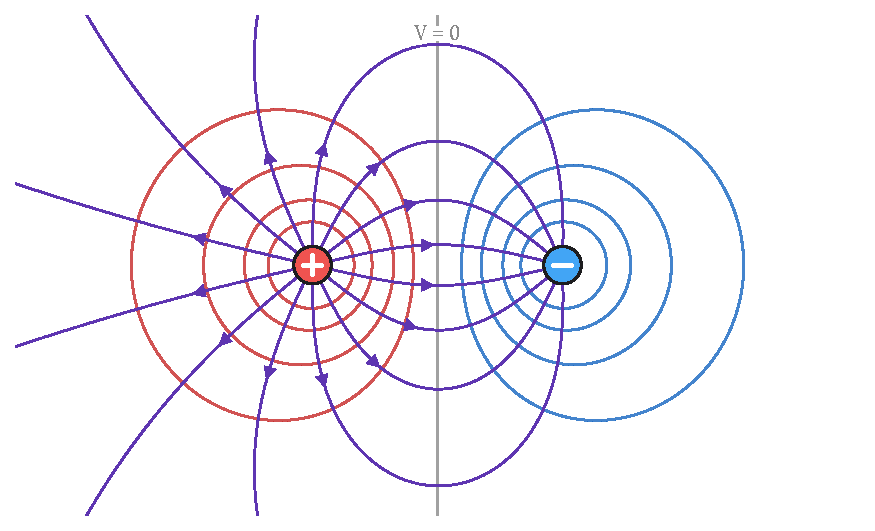
\includegraphics[width=0.66\linewidth]{images/UD5/dipolo}
    \caption{Equipotenciales (positivas en rojo, negativas en azul, \(V = 0\) en gris) y líneas de campo (morado) de un dipolo.
    Se cortan siempre en ángulo recto.}
    \label{fig:ele-dipolo}
\end{figure}

\subsection{Campo uniforme entre placas paralelas}\label{subsec:ele-placas}

Entre dos placas planas paralelas con cargas opuestas el campo es \textbf{uniforme}: tiene el mismo valor en todos los puntos,
va de la placa positiva a la negativa y las equipotenciales son planos paralelos a las placas (figura~\ref{fig:ele-placas}).
Integrando \(dV = -E\,dx\) con \(E\) constante:
\begin{centeredequation}
    \boxed{V_A - V_B = E\,d} \qquad\Rightarrow\qquad E = \dfrac{\Delta V}{d} \label{eq:ele-placas}
\end{centeredequation}
Por eso el campo eléctrico también se mide en \unit{\volt\per\m} (\(\qty{1}{\volt\per\m} = \qty{1}{\newton\per\coulomb}\)).

\begin{figure}[H]
    \centering
    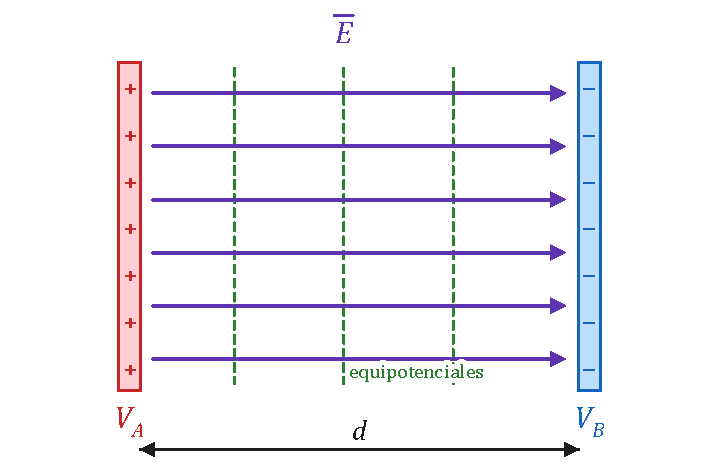
\includegraphics[width=0.5\linewidth]{images/UD5/placas}
    \caption{Campo uniforme entre dos placas paralelas.}
    \label{fig:ele-placas}
\end{figure}

\begin{exercise}
    Dos placas paralelas separadas \qty{5}{\cm} tienen una diferencia de potencial de \qty{6000}{\volt}. Se libera un protón en
    reposo junto a la placa positiva. Calcula el campo entre las placas y la velocidad con que llega el protón a la negativa
    (\(q_p = \qty{1.6e-19}{\coulomb}\), \(m_p = \qty{1.67e-27}{\kg}\)).
    \begin{solu}
        \(E = \dfrac{\Delta V}{d} = \dfrac{6000}{0{,}05} = \textcolor{red}{\qty{1.2e5}{\newton\per\coulomb}}\).

        \textcolor{blue}{El trabajo del campo se convierte en energía cinética: \(q\,\Delta V = \tfrac{1}{2}m v^2\).}
        \(v = \sqrt{\dfrac{2 q\,\Delta V}{m}} = \sqrt{\dfrac{2\cdot 1{,}6\cdot 10^{-19}\cdot 6000}{1{,}67\cdot 10^{-27}}} = \textcolor{red}{\qty{1.07e6}{\m\per\second}}\).
    \end{solu}
\end{exercise}

\subsection{Movimiento de cargas en un campo uniforme}\label{subsec:ele-movimiento}

Sobre una carga en un campo uniforme actúa una fuerza constante \(\vec F = q\vec E\), y su aceleración es \(\vec a = q\vec E/m\):
el problema es igual que el de un tiro en el campo gravitatorio, pero con otra «gravedad». Si una partícula entra con velocidad
\(\vec v_0\) perpendicular al campo, su movimiento es uniforme en la dirección de \(\vec v_0\) y uniformemente acelerado en la
del campo, y describe una \textbf{parábola} (figura~\ref{fig:ele-desviacion}). En esto se basaban los tubos de rayos catódicos de
los televisores antiguos, y se basan las impresoras de chorro de tinta.

\begin{figure}[H]
    \centering
    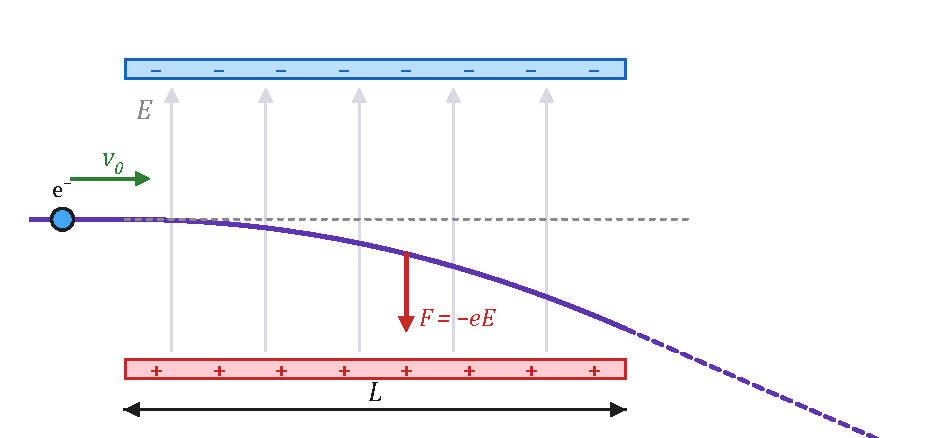
\includegraphics[width=0.66\linewidth]{images/UD5/desviacion}
    \caption{Un electrón que entra horizontalmente en un campo vertical se desvía en sentido contrario al campo.}
    \label{fig:ele-desviacion}
\end{figure}

\begin{exercise}
    Si una carga positiva se mueve en sentido contrario al campo, ¿aumenta o disminuye su energía potencial? ¿Y si es negativa?
    \begin{solu}
        \textcolor{blue}{Al ir en contra del campo va hacia potenciales mayores (\(\Delta V > 0\)), y \(\Delta E_p = q\,\Delta V\).}
        \textcolor{red}{Si es positiva, su energía potencial aumenta} (hay que empujarla); \textcolor{red}{si es negativa, disminuye}
        (ese movimiento es espontáneo para ella).
    \end{solu}
\end{exercise}

\section{Flujo eléctrico y teorema de Gauss}\label{sec:ele-gauss}

\subsection{Flujo del campo eléctrico}\label{subsec:ele-flujo}

El \rojon{flujo} del campo eléctrico a través de una superficie mide el número de líneas de campo que la atraviesan.
Representamos la superficie con un vector \(\vec S\) perpendicular a ella, de módulo igual a su área. Para un campo uniforme y
una superficie plana:
\begin{centeredequation}
    \boxed{\Phi = \vec E\cdot\vec S = E\,S\cos\alpha} \label{eq:ele-flujo}
\end{centeredequation}
El flujo es máximo si la superficie es perpendicular a las líneas (\(\alpha = 0\)) y nulo si es paralela a ellas. Se mide en
\unit{\newton\m\squared\per\coulomb}. Si el campo no es uniforme o la superficie es curva, se divide en elementos \(d\vec S\) y se
suma: \(\Phi = \oint\vec E\cdot d\vec S\). En una superficie cerrada, \(d\vec S\) apunta hacia fuera, así que las líneas que
salen cuentan como flujo positivo y las que entran, como negativo.

\begin{figure}[H]
    \centering
    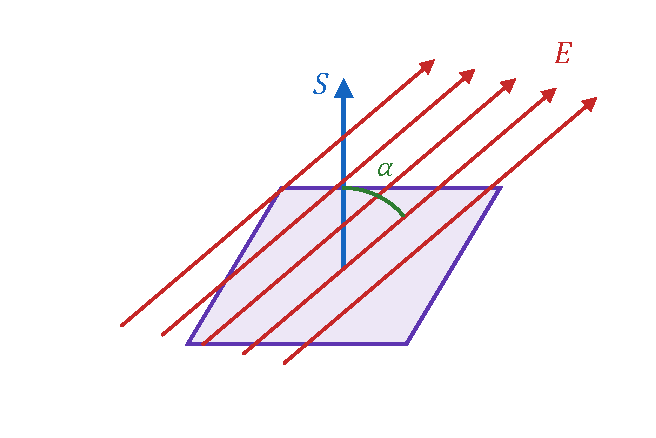
\includegraphics[width=0.45\linewidth]{images/UD5/flujo}
    \caption{El flujo depende del campo, del área y del ángulo \(\alpha\) entre \(\vec E\) y \(\vec S\).}
    \label{fig:ele-flujo}
\end{figure}

\subsection{Teorema de Gauss}\label{subsec:ele-teorema-gauss}

Calculemos el flujo del campo de una carga \(Q\) a través de una esfera de radio \(r\) centrada en ella (una \azuln{superficie
gaussiana}). En cada punto \(\vec E\) es radial, paralelo a \(d\vec S\), y vale \(kQ/r^2\):
\begin{equation*}
    \Phi = \oint E\,dS = \dfrac{kQ}{r^2}\oint dS = \dfrac{kQ}{r^2}\,4\pi r^2 = 4\pi k Q = \dfrac{Q}{\varepsilon_0}
\end{equation*}
El resultado no depende del radio, y como el número de líneas que atraviesan cualquier otra superficie cerrada que rodee la
carga es el mismo, vale para cualquier forma. Sumando para varias cargas:

\begin{definition}[Teorema de Gauss]
    El flujo eléctrico a través de cualquier superficie cerrada es igual a la carga neta encerrada en su interior dividida por
    la permitividad del vacío:
    \begin{centeredequation}
        \boxed{\Phi = \oint\vec E\cdot d\vec S = \dfrac{Q_{\text{int}}}{\varepsilon_0}} \label{eq:ele-gauss}
    \end{centeredequation}
    Las cargas exteriores no contribuyen: sus líneas entran y salen, y su flujo neto es nulo.
\end{definition}

\begin{figure}[H]
    \centering
    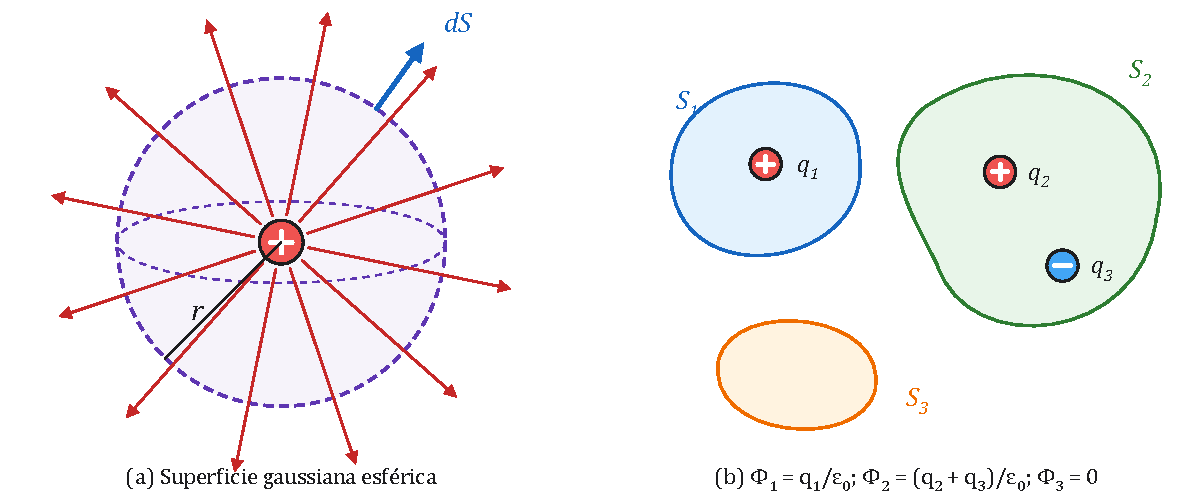
\includegraphics[width=0.95\linewidth]{images/UD5/gauss}
    \caption{(a) Esfera gaussiana alrededor de una carga. (b) El flujo a través de cada superficie cerrada solo depende de la
    carga encerrada.}
    \label{fig:ele-gauss}
\end{figure}

\subsection{Aplicaciones del teorema de Gauss}\label{subsec:ele-aplicaciones}

El teorema de Gauss permite calcular de forma muy sencilla el campo de distribuciones de carga simétricas. Se elige una
superficie gaussiana en la que el campo sea perpendicular a ella y tenga el mismo valor en todos sus puntos (o sea paralelo,
y no aporte flujo).

\paragraph{a) Conductor en equilibrio.} Dentro de un conductor en equilibrio el campo es nulo: si no lo fuera, las cargas
libres se moverían. Por el teorema de Gauss, la carga encerrada por cualquier superficie interior es nula: \textbf{toda la carga
de un conductor se reparte por su superficie}. Además, fuera del conductor el campo es perpendicular a la superficie (si
tuviera una componente paralela, movería las cargas), y todo el conductor está al mismo potencial. Por eso un coche o un
avión son buenos refugios frente a un rayo (\emph{jaula de Faraday}).

\paragraph{b) Esfera cargada.} Fuera de una esfera de radio \(R\) con carga \(Q\), cogiendo una superficie gaussiana esférica
de radio \(r > R\): \(E\cdot 4\pi r^2 = Q/\varepsilon_0\), es decir,
\begin{centeredequation}
    E = k\,\dfrac{Q}{r^2} \qquad (r \geq R) \label{eq:ele-esfera-fuera}
\end{centeredequation}
\textbf{Fuera de ella, una esfera cargada crea el mismo campo que una carga puntual en su centro.} Dentro hay que distinguir:
\begin{itemize}
    \item \emph{Esfera conductora} (o hueca, con la carga en la superficie): la carga encerrada es nula y \(E = 0\) para \(r < R\).
    \item \emph{Esfera maciza aislante con carga uniforme} de densidad \(\rho = Q/\tfrac{4}{3}\pi R^3\): la carga encerrada es
    \(Q\,r^3/R^3\), y queda
    \begin{centeredequation}
        E = k\,\dfrac{Q\,r}{R^3} \qquad (r \leq R) \label{eq:ele-esfera-dentro}
    \end{centeredequation}
    el campo crece linealmente desde el centro, igual que el gravitatorio dentro de la Tierra.
\end{itemize}

\paragraph{c) Hilo indefinido.} Para un hilo recto con densidad lineal de carga \(\lambda = q/L\) se toma un cilindro coaxial
de radio \(r\) y altura \(h\). En las bases el campo es paralelo a la superficie y no hay flujo; en la superficie lateral es
perpendicular y constante (figura~\ref{fig:ele-gauss-aplicaciones}a):
\begin{equation*}
    E\cdot 2\pi r h = \dfrac{\lambda h}{\varepsilon_0} \qquad\Rightarrow\qquad \boxed{E = \dfrac{\lambda}{2\pi\varepsilon_0\,r}}
\end{equation*}

\paragraph{d) Plano indefinido.} Para un plano con densidad superficial de carga \(\sigma = Q/S\), se toma un cilindro que lo
atraviesa. Solo hay flujo por las dos bases (figura~\ref{fig:ele-gauss-aplicaciones}b):
\begin{equation*}
    2\,E\,S = \dfrac{\sigma S}{\varepsilon_0} \qquad\Rightarrow\qquad \boxed{E = \dfrac{\sigma}{2\varepsilon_0}}
\end{equation*}
El campo no depende de la distancia al plano. Entre dos placas paralelas con cargas \(+\sigma\) y \(-\sigma\), los campos de
las dos se suman entre ellas y se anulan fuera: \(E = \sigma/\varepsilon_0\), el campo uniforme del apartado anterior.

\begin{figure}[H]
    \centering
    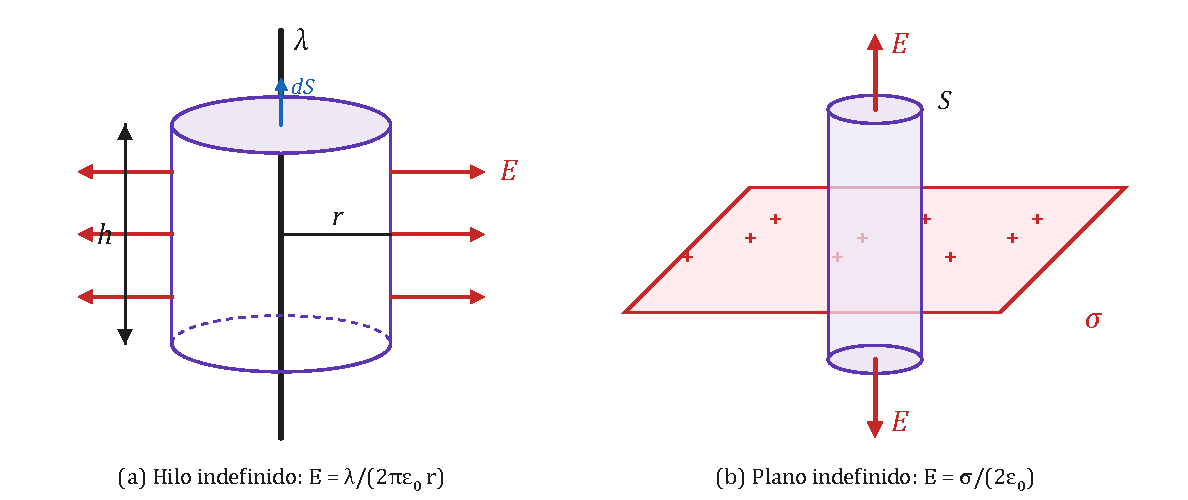
\includegraphics[width=0.95\linewidth]{images/UD5/gauss_aplicaciones}
    \caption{Superficies gaussianas para un hilo y para un plano cargados.}
    \label{fig:ele-gauss-aplicaciones}
\end{figure}

\begin{exercise}
    Una esfera maciza aislante de \qty{15}{\cm} de radio tiene una carga de \qty{6}{\micro\coulomb} repartida uniformemente.
    Calcula, con el teorema de Gauss, el campo a \qty{5}{\cm} y a \qty{20}{\cm} de su centro.
    \begin{solu}
        \(r = \qty{0.05}{\m}\) (dentro): \(E = k\,\dfrac{Q r}{R^3} = 9\cdot 10^9\,\dfrac{6\cdot 10^{-6}\cdot 0{,}05}{0{,}15^3} = \textcolor{red}{\qty{8.0e5}{\newton\per\coulomb}}\).

        \(r = \qty{0.20}{\m}\) (fuera): \(E = k\,\dfrac{Q}{r^2} = \textcolor{red}{\qty{1.35e6}{\newton\per\coulomb}}\).
    \end{solu}
\end{exercise}

\begin{exercise}
    Una esfera hueca conductora de \qty{25}{\cm} de radio tiene una carga de \qty{8}{\micro\coulomb}. Calcula el campo a
    \qty{12}{\cm} y a \qty{40}{\cm} de su centro.
    \begin{solu}
        \textcolor{red}{A \qty{12}{\cm}, \(E = 0\)}: \textcolor{blue}{no hay carga encerrada.}
        A \qty{40}{\cm}: \(E = 9\cdot 10^9\,\dfrac{8\cdot 10^{-6}}{0{,}4^2} = \textcolor{red}{\qty{4.5e5}{\newton\per\coulomb}}\).
    \end{solu}
\end{exercise}

\begin{exercise}
    Un hilo muy largo tiene una carga de \qty{2}{\micro\coulomb} por metro. ¿Cuánto vale el campo a \qty{30}{\cm} de él? ¿Y el
    de una lámina plana muy grande con \qty{5}{\micro\coulomb\per\m\squared}?
    \begin{solu}
        \(E_{\text{hilo}} = \dfrac{\lambda}{2\pi\varepsilon_0 r} = \dfrac{2\cdot 10^{-6}}{2\pi\cdot 8{,}85\cdot 10^{-12}\cdot 0{,}3} = \textcolor{red}{\qty{1.20e5}{\newton\per\coulomb}}\).

        \(E_{\text{plano}} = \dfrac{\sigma}{2\varepsilon_0} = \dfrac{5\cdot 10^{-6}}{2\cdot 8{,}85\cdot 10^{-12}} = \textcolor{red}{\qty{2.82e5}{\newton\per\coulomb}}\), \textcolor{blue}{a cualquier distancia.}
    \end{solu}
\end{exercise}

\section{Esferas conductoras unidas por un hilo}\label{sec:ele-esferas}

El potencial de una esfera conductora de radio \(r\) y carga \(q\) es el de su superficie, \(V = kq/r\). Si se unen dos esferas
con un hilo conductor, pasan cargas de la de mayor potencial a la de menor hasta que los potenciales se igualan
(figura~\ref{fig:ele-esferas}). Las condiciones son:
\begin{centeredequation}
    \text{igualdad de potenciales: } \dfrac{k\,q'_1}{r_1} = \dfrac{k\,q'_2}{r_2} \qquad\qquad \text{conservación de la carga: } q'_1 + q'_2 = q_1 + q_2 \label{eq:ele-esferas}
\end{centeredequation}
La carga final de cada esfera es proporcional a su radio: la esfera grande se queda con más carga, pero la densidad de carga
es mayor en la pequeña. Por eso el campo es más intenso en las zonas puntiagudas de un conductor (\emph{efecto de las puntas},
en el que se basan los pararrayos).

\begin{figure}[H]
    \centering
    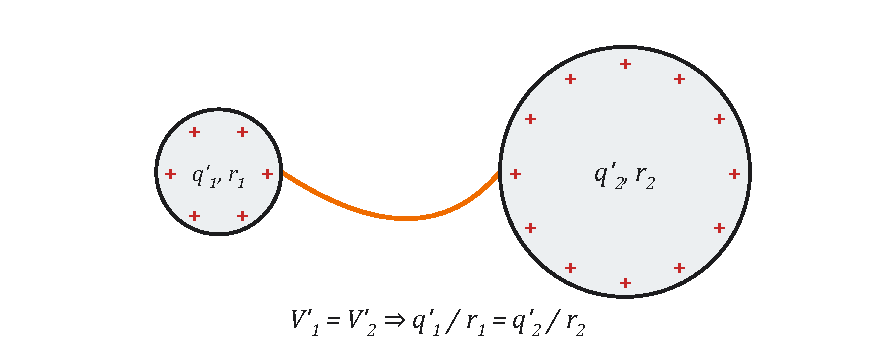
\includegraphics[width=0.62\linewidth]{images/UD5/esferas_hilo}
    \caption{Al unirlas, las dos esferas quedan al mismo potencial.}
    \label{fig:ele-esferas}
\end{figure}

\begin{exercise}
    Dos esferas metálicas de \qty{3}{\cm} y \qty{6}{\cm} de radio tienen cada una una carga de \qty{4e-8}{\coulomb}. Si se unen
    con un hilo conductor, ¿qué carga y qué potencial tendrá cada una?
    \begin{solu}
        \textcolor{blue}{\(q'_1 + q'_2 = \qty{8e-8}{\coulomb}\) y \(q'_1/0{,}03 = q'_2/0{,}06 \Rightarrow q'_2 = 2q'_1\).}
        \(q'_1 = \textcolor{red}{\qty{2.67e-8}{\coulomb}}\); \(q'_2 = \textcolor{red}{\qty{5.33e-8}{\coulomb}}\);
        \(V = 9\cdot 10^9\,\dfrac{2{,}67\cdot 10^{-8}}{0{,}03} = \textcolor{red}{\qty{8000}{\volt}}\) \textcolor{blue}{(las dos).}
    \end{solu}
\end{exercise}

\section{Resumen de fórmulas}\label{sec:ele-resumen}

\begin{table}[H]
    \centering
    \caption{Fórmulas principales del campo eléctrico}
    \vspace{-5pt}
    \begin{tabular}{@{}lL{10cm}@{}}
        \toprule
        \textbf{Magnitud} & \textbf{Expresión} \\
        \midrule
        Ley de Coulomb & \(F = k\,|Q q|/r^2\), \quad \(k = 1/(4\pi\varepsilon_0) = \qty{9e9}{\newton\m\squared\per\coulomb\squared}\) \\[3pt]
        Campo eléctrico & \(E = k\,|Q|/r^2\), \quad \(\vec F = q\vec E\) \\[3pt]
        Energía potencial & \(E_p = kQq/r\) (con signos) \\[3pt]
        Potencial & \(V = kQ/r\), \quad \(V = \sum V_i\), \quad \(W_{A\to B} = q(V_A - V_B)\) \\[3pt]
        Campo y potencial & \(E_x = -dV/dx\); \quad campo uniforme: \(V_A - V_B = E\,d\) \\[3pt]
        Flujo & \(\Phi = \vec E\cdot\vec S = E S\cos\alpha\) \\[3pt]
        Teorema de Gauss & \(\Phi = Q_{\text{int}}/\varepsilon_0\) \\[3pt]
        Esfera de carga \(Q\) & fuera: \(E = kQ/r^2\); \quad dentro: conductora \(E = 0\), maciza \(E = kQr/R^3\) \\[3pt]
        Hilo y plano & \(E = \lambda/(2\pi\varepsilon_0 r)\); \quad \(E = \sigma/(2\varepsilon_0)\) \\[3pt]
        Esferas unidas & \(q'_1/r_1 = q'_2/r_2\), \quad \(q'_1 + q'_2 = q_1 + q_2\) \\
        \bottomrule
    \end{tabular}
    \label{tab:ele-resumen}
\end{table}

\begin{table}[H]
    \centering
    \caption{Comparación entre el campo gravitatorio y el eléctrico}
    \vspace{-5pt}
    \begin{tabular}{@{}lL{5.4cm}L{5.4cm}@{}}
        \toprule
        & \textbf{Gravitatorio} & \textbf{Eléctrico} \\
        \midrule
        Lo crea & la masa & la carga \\[3pt]
        Fuerza & siempre atractiva & atractiva o repulsiva \\[3pt]
        Constante & \(G\), universal y muy pequeña & \(k\), depende del medio y es muy grande \\[3pt]
        Líneas de campo & solo llegan a las masas & salen de las cargas positivas y llegan a las negativas \\[3pt]
        Potencial & \(V = -GM/r\), siempre negativo & \(V = kQ/r\), con el signo de \(Q\) \\[3pt]
        En común & \multicolumn{2}{L{10.8cm}}{Fuerzas centrales, conservativas e inversamente proporcionales al cuadrado de la distancia} \\
        \bottomrule
    \end{tabular}
    \label{tab:ele-comparacion}
\end{table}

\section{Prácticas de laboratorio}\label{sec:ele-practicas}

\subsection{Práctica 1: superficies equipotenciales en una cubeta}\label{subsec:ele-practica-cubeta}

\noindent\begin{minipage}[t]{0.56\linewidth}
\textbf{Objetivo.} Localizar las líneas equipotenciales entre dos electrodos y dibujar a partir de ellas las líneas de campo.

\textbf{Material.} Cubeta de fondo plano con una capa de agua del grifo de 1 o 2 cm, papel milimetrado debajo, dos electrodos
(láminas metálicas o clavos gruesos), fuente de corriente continua de 6 a 12 V, voltímetro digital y cables.

\textbf{Procedimiento.}
\begin{enumerate}[label=\numberballmDarkTeal]
    \item Conecta los electrodos a la fuente y el terminal negativo del voltímetro al electrodo negativo
    (figura~\ref{fig:ele-practica}).
    \item Con la otra punta del voltímetro, busca varios puntos en los que marque, por ejemplo, \qty{3}{\volt} y anota sus
    coordenadas en el papel. Repite con \qty{6}{\volt} y \qty{9}{\volt}.
    \item Une los puntos de igual potencial y dibuja las líneas de campo perpendiculares a ellos.
    \item Repite con dos electrodos puntuales (clavos).
\end{enumerate}
\end{minipage}\hfill
\begin{minipage}[t]{0.4\linewidth}
    \vspace{0pt}
    \centering
    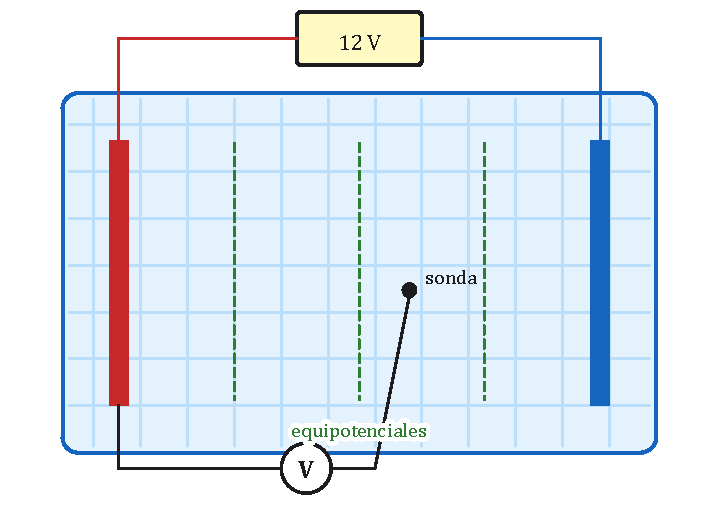
\includegraphics[width=\linewidth]{images/UD5/practica_equipotenciales}
    \captionof{figure}{Montaje con dos electrodos planos.}
    \label{fig:ele-practica}
\end{minipage}

\textbf{Cuestiones.}
\begin{enumerate}[label=\letraminuscula]
    \item Con los electrodos planos, ¿cómo son las equipotenciales? ¿Están igual de separadas? Calcula el campo con \(E = \Delta V/d\).
    \item Compara el mapa de los electrodos puntuales con la figura~\ref{fig:ele-dipolo}.
    \item ¿Por qué no circula apenas corriente por el voltímetro? ¿Por qué hay que usar agua del grifo y no agua destilada?
\end{enumerate}

\subsection{Práctica 2: el péndulo eléctrico}\label{subsec:ele-practica-pendulo}

\noindent\begin{minipage}[t]{0.6\linewidth}
\textbf{Objetivo.} Observar la electrización por frotamiento, contacto e inducción y estimar la carga de una bolita.

\textbf{Material.} Bolita de papel de aluminio (o de corcho blanco recubierta) colgada de un hilo de seda o de nailon de unos
\qty{30}{\cm}, varillas de plástico y de vidrio, paño de lana, balanza de precisión y regla.

\textbf{Procedimiento.}
\begin{enumerate}[label=\numberballmDarkTeal]
    \item Frota la varilla de plástico y acércala a la bolita sin tocarla: observa que la atrae (inducción).
    \item Deja que la toque: después la repele (contacto). Repite con la de vidrio y compara.
    \item Carga por contacto dos bolitas iguales colgadas del mismo punto y mide el ángulo que forman sus hilos en el equilibrio.
\end{enumerate}
\end{minipage}\hfill
\begin{minipage}[t]{0.36\linewidth}
    \vspace{0pt}
    \centering
    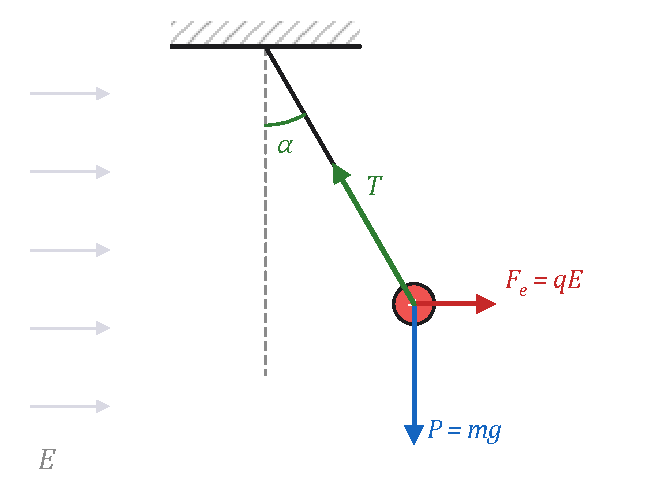
\includegraphics[width=\linewidth]{images/UD5/pendulo_electrico}
    \captionof{figure}{Fuerzas sobre una bolita cargada en equilibrio.}
    \label{fig:ele-pendulo}
\end{minipage}

\textbf{Cálculos.} En el equilibrio, \(T\cos\alpha = mg\) y \(T\sen\alpha = F_e\), así que \(F_e = mg\tg\alpha\). Con
\(F_e = k\,q^2/r^2\) y la separación \(r\) entre las bolitas, estima su carga.

\textbf{Cuestiones.}
\begin{enumerate}[label=\letraminuscula]
    \item ¿Por qué la bolita neutra es atraída por la varilla aunque no tenga carga neta?
    \item ¿Por qué la experiencia sale peor un día húmedo?
    \item ¿De qué orden es la carga obtenida? Exprésala en número de electrones.
\end{enumerate}


    \newpage

    %! Unidad 5 — Campo eléctrico: ejercicios finales (adaptados de la fuente, con datos cambiados y resueltos)

\section{Ejercicios}\label{sec:ele-ejercicios}

Salvo que se indique otra cosa, usa \(k = \qty{9e9}{\newton\m\squared\per\coulomb\squared}\), \(e = \qty{1.6e-19}{\coulomb}\),
\(m_p = \qty{1.67e-27}{\kg}\), \(m_e = \qty{9.11e-31}{\kg}\) y \(g = \qty{9.8}{\m\per\second\squared}\).

\subsection{Cuestiones}

\begin{exercise}
    Si en un punto entre dos cargas el campo eléctrico es nulo, ¿qué puedes decir de los signos de las cargas? ¿Y si el punto
    está fuera del segmento que las une?
    \begin{solu}
        \textcolor{blue}{Entre las cargas, el campo de cada una apunta en sentidos opuestos solo si tienen el mismo signo.}
        \textcolor{red}{Si el punto está entre ellas, son del mismo signo; si está fuera del segmento, son de signo contrario}
        \textcolor{blue}{(y el punto está más cerca de la de menor valor absoluto).}
    \end{solu}
\end{exercise}

\begin{exercise}
    ¿En qué punto (aparte del infinito) no experimentaría fuerza una tercera carga colocada cerca de dos cargas iguales?
    \begin{solu}
        \textcolor{red}{En el punto medio del segmento que las une}: \textcolor{blue}{allí los campos de las dos son iguales y opuestos.}
    \end{solu}
\end{exercise}

\begin{exercise}
    ¿Cuánto trabajo cuesta llevar una carga de un punto a otro de la misma superficie equipotencial?
    \begin{solu}
        \textcolor{red}{Ninguno}: \(W = q(V_A - V_B) = 0\) \textcolor{blue}{porque \(V_A = V_B\). El campo es perpendicular al desplazamiento.}
    \end{solu}
\end{exercise}

\begin{exercise}
    Se libera un protón en reposo en un campo eléctrico uniforme. ¿Aumenta o disminuye su energía potencial? ¿Y si fuera un electrón?
    \begin{solu}
        \textcolor{red}{En los dos casos disminuye}: \textcolor{blue}{todo movimiento espontáneo desde el reposo convierte energía
        potencial en cinética. El protón va hacia potenciales menores y el electrón, hacia potenciales mayores.}
    \end{solu}
\end{exercise}

\begin{exercise}
    Una partícula se mueve en el sentido de un campo eléctrico y su energía potencial aumenta. ¿Qué signo tiene su carga?
    \begin{solu}
        \textcolor{blue}{En el sentido del campo el potencial disminuye (\(\Delta V < 0\)). Como \(\Delta E_p = q\,\Delta V > 0\):}
        \textcolor{red}{\(q < 0\)}.
    \end{solu}
\end{exercise}

\begin{exercise}
    En un punto \(A\) el potencial es \qty{25}{\volt} y en otro \(B\), \qty{10}{\volt}. ¿Hacia dónde se moverá espontáneamente una
    carga positiva? Si es de \qty{3}{\coulomb} y parte del reposo, ¿qué energía cinética tendrá al llegar?
    \begin{solu}
        \textcolor{red}{De \(A\) a \(B\)}, \textcolor{blue}{hacia potenciales menores.}
        \(E_c = W = q(V_A - V_B) = 3\cdot 15 = \textcolor{red}{\qty{45}{\joule}}\).
    \end{solu}
\end{exercise}

\subsection{Fuerzas y campos}

\begin{exercise}
    Una carga de \qty{4}{\micro\coulomb} está en el origen y otra de \qty{-6}{\micro\coulomb} en \((12, 0)\) cm. Calcula el campo
    en el punto \(B\) situado en la vertical de la segunda carga, de forma que la recta que lo une con la primera forma \ang{30}
    con el eje \(X\).
    \begin{solu}
        \textcolor{blue}{\(B = (12;\ 12\tg\ang{30}) = (12;\ 6{,}93)\) cm. Distancias: \(r_1 = \qty{13.9}{\cm}\), \(r_2 = \qty{6.93}{\cm}\).}

        \(E_1 = k\,\dfrac{4\cdot 10^{-6}}{0{,}1386^2} = \qty{1.88e6}{\newton\per\coulomb}\), \textcolor{blue}{alejándose del origen a \ang{30}};
        \(E_2 = k\,\dfrac{6\cdot 10^{-6}}{0{,}0693^2} = \qty{1.13e7}{\newton\per\coulomb}\), \textcolor{blue}{hacia abajo.}
        \[ \textcolor{red}{\vec E = (1{,}62\,\vec{i} - 10{,}3\,\vec{j})\cdot 10^6\ \unit{\newton\per\coulomb}};\quad E = \textcolor{red}{\qty{1.04e7}{\newton\per\coulomb}} \]
    \end{solu}
\end{exercise}

\begin{exercise}
    Una carga de \qty{3}{\micro\coulomb} está en \((2, 0)\) y otra de \qty{-2}{\micro\coulomb} en \((0, 1)\), con las coordenadas en
    centímetros. Calcula el campo y el potencial en el punto \((1, 2)\).
    \begin{solu}
        \textcolor{blue}{Distancias: \(r_1 = \sqrt 5\ \unit{\cm}\), \(r_2 = \sqrt 2\ \unit{\cm}\). Con \(\vec E_i = k q_i\,\vec r_i/r_i^3\):}
        \[ \textcolor{red}{\vec E = (-8{,}78\,\vec{i} - 1{,}53\,\vec{j})\cdot 10^7\ \unit{\newton\per\coulomb}} \qquad
           V = 9\cdot 10^9\left(\dfrac{3\cdot 10^{-6}}{0{,}02236} - \dfrac{2\cdot 10^{-6}}{0{,}01414}\right) = \textcolor{red}{\qty{-6.5e4}{\volt}} \]
    \end{solu}
\end{exercise}

\begin{exercise}
    Tres cargas de \qty{2e-6}{\coulomb} están en los puntos \((-1, 0)\), \((1, 1)\) y \((0, 1)\) (en metros). Calcula el campo en el
    origen y la energía potencial del sistema.
    \begin{solu}
        \[ \textcolor{red}{\vec E = (1{,}16\,\vec{i} - 2{,}44\,\vec{j})\cdot 10^4\ \unit{\newton\per\coulomb}};\quad E = \textcolor{red}{\qty{2.70e4}{\newton\per\coulomb}} \]
        \(E_p = k q^2\left(\dfrac{1}{\sqrt 5} + \dfrac{1}{\sqrt 2} + 1\right) = \textcolor{red}{\qty{7.76e-2}{\joule}}\).
    \end{solu}
\end{exercise}

\begin{exercise}
    Tres cargas de \qty{2}{\micro\coulomb} están en \((0, 0)\), \((0, 40)\) y \((30, 0)\) cm. Calcula la fuerza sobre otra carga igual
    situada en \((30, 40)\) cm.
    \begin{solu}
        \textcolor{blue}{Las tres repelen. La de \((0, 40)\), a \qty{0.3}{\m}, empuja hacia \(+X\): \qty{0.40}{\newton}; la de \((30, 0)\), a \qty{0.4}{\m},
        hacia \(+Y\): \qty{0.225}{\newton}; la del origen, a \qty{0.5}{\m}, \qty{0.144}{\newton} en la dirección \((0{,}6;\,0{,}8)\).}
        \[ \textcolor{red}{\vec F = 0{,}486\,\vec{i} + 0{,}340\,\vec{j}\ \unit{\newton}};\quad F = \textcolor{red}{\qty{0.594}{\newton}} \]
    \end{solu}
\end{exercise}

\begin{exercise}
    Dos bolitas de \qty{0.4}{\g} cuelgan de un mismo punto con hilos de \qty{40}{\cm}. Tienen la misma carga y en el equilibrio
    los hilos forman entre sí \ang{30}. Calcula la carga de cada una.
    \begin{solu}
        \textcolor{blue}{Cada hilo forma \ang{15} con la vertical; las bolitas están a \(r = 2\cdot 0{,}4\sen\ang{15} = \qty{0.207}{\m}\).
        En el equilibrio \(F_e = mg\tg\ang{15} = \qty{1.05e-3}{\newton}\).}
        \(q = r\sqrt{\dfrac{F_e}{k}} = \textcolor{red}{\qty{7.1e-8}{\coulomb}}\).
    \end{solu}
\end{exercise}

\begin{exercise}
    Representa las líneas de campo de dos cargas \(+3q\) y \(-q\).
    \begin{solu}
        \textcolor{blue}{Como en la figura~\ref{fig:ele-lineas}e:} \textcolor{red}{salen de \(+3q\) el triple de líneas de las que llegan a \(-q\); la tercera
        parte termina en \(-q\) y el resto se va al infinito.} \textcolor{blue}{Lejos de las dos, el campo es como el de una carga \(+2q\).}
    \end{solu}
\end{exercise}

\subsection{Potencial y energía}

\begin{exercise}
    Una carga de \qty{5}{\micro\coulomb} está en el origen.
    \begin{enumerate}[label=\letraminuscula]
        \item ¿Cuánto vale el potencial a \qty{2}{\m}?
        \item ¿Qué trabajo hay que hacer para traer desde el infinito hasta allí una carga de \qty{3}{\micro\coulomb}?
        \item ¿Qué energía potencial tiene esa carga en esa posición?
    \end{enumerate}
    \begin{solu}
        \begin{enumerate}[label=\letraminuscula]
            \item \(V = k\,\dfrac{Q}{r} = \textcolor{red}{\qty{2.25e4}{\volt}}\).
            \item \(W_{\text{ext}} = q\,(V - 0) = \textcolor{red}{\qty{6.75e-2}{\joule}}\).
            \item \(E_p = qV = \textcolor{red}{\qty{6.75e-2}{\joule}}\) \textcolor{blue}{(coincide con el trabajo exterior).}
        \end{enumerate}
    \end{solu}
\end{exercise}

\begin{exercise}
    Tres cargas \(q_1 = \qty{3}{\micro\coulomb}\), \(q_2 = \qty{5}{\micro\coulomb}\) y \(q_3 = \qty{-6}{\micro\coulomb}\) están en
    \((0, 0)\), \((6, 0)\) y \((3, 0)\) (en metros). Calcula:
    \begin{enumerate}[label=\letraminuscula]
        \item El campo en \(A(3, 3)\).
        \item El potencial en \(A\) y en \(B(0, 3)\) y el trabajo del campo al llevar una carga de \qty{2}{\micro\coulomb} de \(A\) a \(B\).
        \item El trabajo exterior para llevarla de \(B\) a \(A\).
    \end{enumerate}
    \begin{solu}
        \begin{enumerate}[label=\letraminuscula]
            \item \(\textcolor{red}{\vec E = -707\,\vec{i} - 3172\,\vec{j}\ \unit{\newton\per\coulomb}}\).
            \item \(V_A = k\left(\dfrac{3}{\sqrt{18}} + \dfrac{5}{\sqrt{18}} - \dfrac{6}{3}\right)\cdot 10^{-6} = \textcolor{red}{\qty{-1029}{\volt}}\);
            \(V_B = k\left(\dfrac{3}{3} + \dfrac{5}{\sqrt{45}} - \dfrac{6}{\sqrt{18}}\right)\cdot 10^{-6} = \textcolor{red}{\qty{2980}{\volt}}\).

            \(W_{A\to B} = q(V_A - V_B) = \textcolor{red}{\qty{-8.0e-3}{\joule}}\).
            \item \(W_{\text{ext},B\to A} = q(V_A - V_B) = \textcolor{red}{\qty{-8.0e-3}{\joule}}\): \textcolor{blue}{de \(B\) a \(A\) la carga va sola y el agente externo tiene que frenarla.}
        \end{enumerate}
    \end{solu}
\end{exercise}

\begin{exercise}
    Dos esferas conductoras de \qty{4}{\cm} y \qty{12}{\cm} de radio están a potenciales de \qty{900}{\volt} y \qty{-900}{\volt}, con
    sus centros separados \qty{1.5}{\m}. Calcula la fuerza entre ellas y la carga y el potencial de cada una después de unirlas
    con un hilo conductor.
    \begin{solu}
        \textcolor{blue}{\(q = Vr/k\):} \(q_1 = \qty{4e-9}{\coulomb}\), \(q_2 = \qty{-1.2e-8}{\coulomb}\);
        \(F = k\,\dfrac{|q_1 q_2|}{r^2} = \textcolor{red}{\qty{1.92e-7}{\newton}}\) \textcolor{red}{(atractiva)}.

        \textcolor{blue}{Carga total \qty{-8e-9}{\coulomb}, repartida en proporción a los radios (1:3):}
        \(q'_1 = \textcolor{red}{\qty{-2e-9}{\coulomb}}\), \(q'_2 = \textcolor{red}{\qty{-6e-9}{\coulomb}}\); \(V' = \textcolor{red}{\qty{-450}{\volt}}\).
    \end{solu}
\end{exercise}

\begin{exercise}
    Dos esferas metálicas de \qty{5}{\cm} y \qty{10}{\cm} de radio se cargan con \qty{2e-6}{\coulomb} cada una y luego se unen con un
    hilo conductor. Calcula el potencial y la carga de cada una después de unirlas.
    \begin{solu}
        \(q'_1 = 4\cdot 10^{-6}\,\dfrac{5}{15} = \textcolor{red}{\qty{1.33e-6}{\coulomb}}\); \(q'_2 = \textcolor{red}{\qty{2.67e-6}{\coulomb}}\);
        \(V = k\,\dfrac{q'_1}{r_1} = \textcolor{red}{\qty{2.4e5}{\volt}}\).
    \end{solu}
\end{exercise}

\subsection{Campos uniformes y movimiento de cargas}

\begin{exercise}
    En un campo uniforme de \qty{8000}{\newton\per\coulomb} se libera un protón junto a la placa positiva. ¿Con qué velocidad llega a
    la negativa, situada a \qty{25}{\cm}?
    \begin{solu}
        \(\tfrac{1}{2}m v^2 = qEd \Rightarrow v = \sqrt{\dfrac{2\cdot 1{,}6\cdot 10^{-19}\cdot 8000\cdot 0{,}25}{1{,}67\cdot 10^{-27}}} = \textcolor{red}{\qty{6.19e5}{\m\per\second}}\).
    \end{solu}
\end{exercise}

\begin{exercise}
    Se conectan a una batería de \qty{300}{\volt} dos láminas paralelas separadas \qty{1.5}{\cm}. ¿Cuánto vale el campo entre ellas?
    ¿Qué fuerza ejerce sobre un electrón?
    \begin{solu}
        \(E = \dfrac{300}{0{,}015} = \textcolor{red}{\qty{2e4}{\newton\per\coulomb}}\); \(F = eE = \textcolor{red}{\qty{3.2e-15}{\newton}}\),
        \textcolor{blue}{hacia la placa positiva.}
    \end{solu}
\end{exercise}

\begin{exercise}
    Un electrón entra con velocidad horizontal \(v_0\) en un campo uniforme vertical dirigido hacia arriba. Halla la ecuación de su trayectoria.
    \begin{solu}
        \textcolor{blue}{La fuerza \(-eE\) va hacia abajo; aceleración \(a = eE/m\). Con el origen en el punto de entrada:}
        \(x = v_0 t\); \(y = -\dfrac{1}{2}\,\dfrac{eE}{m}\,t^2\) \(\Rightarrow\)
        \[ \textcolor{red}{y = -\dfrac{eE}{2 m v_0^2}\,x^2} \]
        \textcolor{red}{Es una parábola} \textcolor{blue}{(figura~\ref{fig:ele-desviacion}).}
    \end{solu}
\end{exercise}

\begin{exercise}
    Una esfera de \qty{4}{\g} tiene una carga de \qty{-3}{\micro\coulomb}. ¿Qué campo hay que aplicar para que se mantenga en reposo sin caer?
    \begin{solu}
        \(|q|E = mg \Rightarrow E = \dfrac{0{,}004\cdot 9{,}8}{3\cdot 10^{-6}} = \textcolor{red}{\qty{1.31e4}{\newton\per\coulomb}}\),
        \textcolor{red}{vertical y hacia abajo} \textcolor{blue}{(la carga es negativa: la fuerza va en sentido contrario al campo).}
    \end{solu}
\end{exercise}

\begin{exercise}
    Una esfera de \qty{5}{\mg} colgada de un hilo está en un campo de \(5000\,\vec{i}\ \unit{\newton\per\coulomb}\) y en el equilibrio
    el hilo forma \ang{30} con la vertical. ¿Cuánto vale su carga?
    \begin{solu}
        \(qE = mg\tg\ang{30} \Rightarrow q = \dfrac{5\cdot 10^{-6}\cdot 9{,}8\cdot 0{,}577}{5000} = \textcolor{red}{\qty{5.7e-9}{\coulomb}}\) \textcolor{red}{(positiva)}.
    \end{solu}
\end{exercise}

\begin{exercise}
    Una esfera de \qty{0.4}{\g} con una carga de \qty{0.2}{\micro\coulomb} cuelga de un hilo de \qty{10}{\cm} dentro de un campo
    uniforme de \(6000\,\vec{i}\ \unit{\newton\per\coulomb}\). ¿Qué ángulo forma el hilo con la vertical y cuál es su tensión?
    \begin{solu}
        \(\tg\alpha = \dfrac{qE}{mg} = \dfrac{1{,}2\cdot 10^{-3}}{3{,}92\cdot 10^{-3}} \Rightarrow \textcolor{red}{\alpha = \ang{17.0}}\);
        \(T = \sqrt{(qE)^2 + (mg)^2} = \textcolor{red}{\qty{4.1e-3}{\newton}}\).
    \end{solu}
\end{exercise}

\begin{exercise}
    Una esfera de \qty{40}{\g} sujeta de un hilo está en un campo \(\vec E = (6\,\vec{i} + 8\,\vec{j})\cdot 10^5\ \unit{\newton\per\coulomb}\).
    En el equilibrio el hilo se separa \ang{25} de la vertical. Calcula la carga y la tensión del hilo.
    \begin{solu}
        \textcolor{blue}{Horizontal: \(qE_x = T\sen\alpha\). Vertical: \(qE_y + T\cos\alpha = mg\). Eliminando \(T\):}
        \[ q = \dfrac{mg\tg\alpha}{E_x + E_y\tg\alpha} = \textcolor{red}{\qty{1.88e-7}{\coulomb}} \qquad T = \dfrac{qE_x}{\sen\alpha} = \textcolor{red}{\qty{0.267}{\newton}} \]
    \end{solu}
\end{exercise}

\begin{exercise}
    Una esfera de \qty{0.5}{\g} con una carga de \qty{6}{\micro\coulomb} cuelga entre dos láminas verticales separadas \qty{12}{\cm}.
    En el equilibrio el hilo forma \ang{30} con la vertical (\(g = \qty{9.81}{\m\per\second\squared}\)).
    \begin{enumerate}[label=\letraminuscula]
        \item Dibuja las fuerzas e indica el signo de las placas.
        \item Calcula la tensión del hilo y el campo.
        \item ¿Qué diferencia de potencial hay entre las placas?
    \end{enumerate}
    \begin{solu}
        \begin{enumerate}[label=\letraminuscula]
            \item \textcolor{blue}{Peso, tensión y fuerza eléctrica (figura~\ref{fig:ele-pendulo}). La carga es positiva y se desvía hacia la placa
            negativa}: \textcolor{red}{la placa de la que se aleja es la positiva.}
            \item \(T = \dfrac{mg}{\cos\ang{30}} = \textcolor{red}{\qty{5.66e-3}{\newton}}\); \(E = \dfrac{mg\tg\ang{30}}{q} = \textcolor{red}{\qty{472}{\newton\per\coulomb}}\).
            \item \(\Delta V = E d = \textcolor{red}{\qty{56.6}{\volt}}\).
        \end{enumerate}
    \end{solu}
\end{exercise}

\begin{exercise}
    Entre dos placas horizontales separadas \qty{2}{\cm} hay una diferencia de potencial de \qty{4000}{\volt}, con la positiva abajo.
    \begin{enumerate}[label=\letraminuscula]
        \item ¿Cuánto vale el campo?
        \item Se introduce una bolita con una carga de \qty{3e-7}{\coulomb} colgada de un hilo y la tensión del hilo resulta nula. ¿Qué masa tiene?
        \item Si se invierte la polaridad de las placas, ¿cuánto vale la tensión?
    \end{enumerate}
    \begin{solu}
        \begin{enumerate}[label=\letraminuscula]
            \item \(E = \dfrac{4000}{0{,}02} = \textcolor{red}{\qty{2e5}{\newton\per\coulomb}}\), \textcolor{blue}{hacia arriba.}
            \item \textcolor{blue}{La fuerza eléctrica (hacia arriba) equilibra el peso:} \(m = \dfrac{qE}{g} = \textcolor{red}{\qty{6.1e-3}{\kg} = \qty{6.1}{\g}}\).
            \item \textcolor{blue}{Ahora las dos fuerzas van hacia abajo:} \(T = mg + qE = \textcolor{red}{\qty{0.12}{\newton}}\).
        \end{enumerate}
    \end{solu}
\end{exercise}

\begin{exercise}
    Entre dos placas horizontales separadas \qty{20}{\cm} hay un muelle de constante \qty{50}{\newton\per\m} del que cuelga una bolita
    cargada. Al aplicar \qty{800}{\volt}, con la placa superior positiva, el muelle se alarga \qty{8}{\cm} más.
    \begin{enumerate}[label=\letraminuscula]
        \item Explica el alargamiento y dibuja las fuerzas.
        \item Calcula la carga de la bolita y su signo.
        \item La bolita pierde carga poco a poco: a los \qty{25}{\minute} el alargamiento extra es de \qty{5}{\cm}. ¿A qué ritmo se pierde la carga?
    \end{enumerate}
    \begin{solu}
        \begin{enumerate}[label=\letraminuscula]
            \item \textcolor{blue}{El campo va hacia abajo (de la placa positiva a la negativa). Si el muelle se alarga, la fuerza eléctrica va hacia abajo,
            igual que el campo}: \textcolor{red}{la carga es positiva}.
            \item \(E = \dfrac{800}{0{,}2} = \qty{4000}{\newton\per\coulomb}\); \(qE = k\,\Delta x \Rightarrow q = \dfrac{50\cdot 0{,}08}{4000} = \textcolor{red}{\qty{1e-3}{\coulomb}}\).
            \item \(q' = \dfrac{50\cdot 0{,}05}{4000} = \qty{6.25e-4}{\coulomb}\); \(\dfrac{\Delta q}{\Delta t} = \dfrac{3{,}75\cdot 10^{-4}}{25} = \textcolor{red}{\qty{1.5e-5}{\coulomb\per\minute}}\).
        \end{enumerate}
    \end{solu}
\end{exercise}


%------------------------------------------------

    \chapterimage{images/portada_cabeceras/cabecera_UD6}
    \chapter{Campo magnético e inducción electromagnética}

    %! Unidad 6 — Campo magnético e inducción electromagnética (teoría, actividades resueltas y prácticas)
%! Fuente: Fuentes/Tema_6.pdf (reescrito; datos de las actividades cambiados y recalculados)

\section*{Para empezar: la aguja que se movió}
\addcontentsline{toc}{section}{Para empezar: la aguja que se movió}

En 1820, durante una clase en Copenhague, Hans Christian Oersted conectó un circuito junto a una brújula y vio cómo la aguja
giraba. Hasta entonces la electricidad y el magnetismo se consideraban fenómenos distintos; aquel pequeño giro demostró que
una corriente eléctrica crea un campo magnético. Once años después, Michael Faraday descubrió el efecto contrario: un campo
magnético que cambia produce una corriente. De esas dos ideas salen los motores, los generadores de las centrales, los
transformadores, los altavoces o las placas de inducción de la cocina. En esta unidad estudiaremos el campo magnético, la
fuerza que ejerce sobre cargas y corrientes, cómo lo crean las corrientes y cómo, al variar, induce corrientes eléctricas.

\section{Imanes y campo magnético}\label{sec:mag-imanes}

El \rojon{magnetismo} es la propiedad de algunos cuerpos, como la magnetita (\ch{Fe3O4}), de atraer el hierro. Los imanes
pueden ser naturales o artificiales (piezas de acero imantadas). Sus propiedades básicas son:
\begin{itemize}
    \item El magnetismo es más intenso en los extremos, los \azuln{polos}. Un imán que puede girar libremente orienta uno de
    ellos hacia el norte geográfico: es su \emph{polo norte}. El otro es el \emph{polo sur}.
    \item Los polos del mismo nombre se repelen y los de distinto nombre se atraen. Por eso el polo norte de una brújula
    señala el norte geográfico: allí está el polo \emph{sur} magnético de la Tierra.
    \item \textbf{No se pueden separar los polos}: si se parte un imán, cada trozo es un imán completo con sus dos polos. No
    existen «cargas magnéticas» aisladas.
\end{itemize}

La región que rodea un imán, en la que se notan sus efectos, es su \rojon{campo magnético}. Es un campo vectorial que se
representa con el vector \azuln{inducción magnética} \(\vec B\) (o, simplemente, campo magnético). Sus líneas de campo salen del
polo norte, entran por el polo sur y continúan por dentro del imán: \textbf{son líneas cerradas}, sin principio ni fin
(figura~\ref{fig:mag-iman}).

\begin{figure}[H]
    \centering
    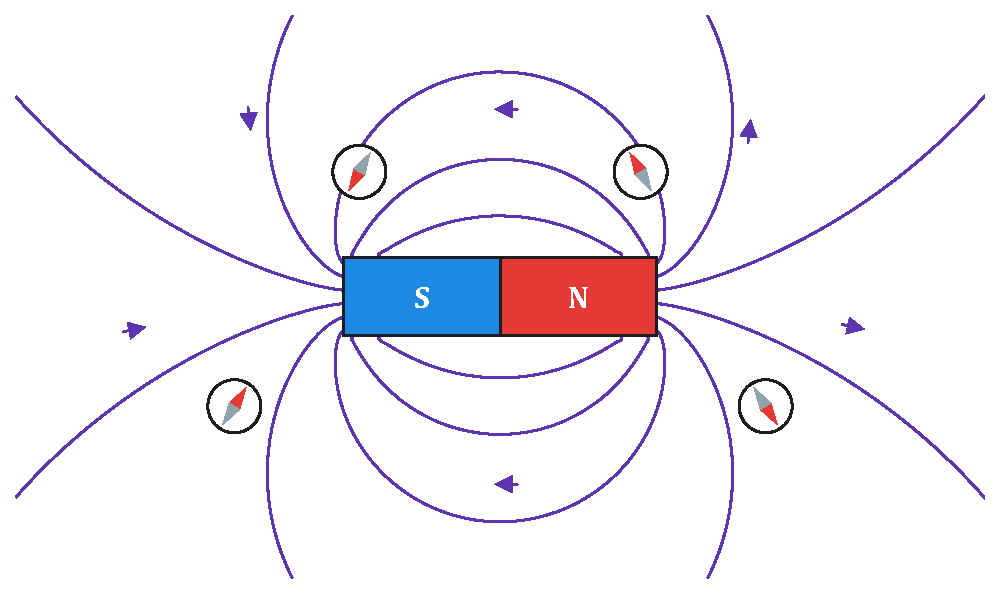
\includegraphics[width=0.7\linewidth]{images/UD6/iman}
    \caption{Líneas del campo de un imán de barra. Las brújulas se orientan tangentes a ellas, con su polo norte (rojo) en el
    sentido del campo.}
    \label{fig:mag-iman}
\end{figure}

\paragraph{Origen del magnetismo natural.} En los átomos, los electrones giran alrededor del núcleo y sobre sí mismos: cada
átomo es un pequeño imán. En la mayoría de los materiales estos imanes elementales están orientados al azar y se anulan. Según
su comportamiento, las sustancias son:
\begin{itemize}
    \item \textbf{Ferromagnéticas} (hierro, cobalto, níquel): son atraídas fuertemente por un imán y se imantan con facilidad.
    \item \textbf{Paramagnéticas} (aluminio, platino, cromo): son atraídas débilmente y no quedan imantadas.
    \item \textbf{Diamagnéticas} (cobre, plata, oro, agua): son repelidas débilmente.
\end{itemize}

\paragraph{La experiencia de Oersted.} Si se coloca una brújula debajo de un hilo orientado en la dirección norte-sur, al pasar
corriente la aguja gira hasta quedar perpendicular al hilo, y al cortarla vuelve a su posición (figura~\ref{fig:mag-oersted}).
\textbf{Las cargas en movimiento crean campos magnéticos.} Todo el magnetismo, también el de los imanes, tiene este origen.

\begin{figure}[H]
    \centering
    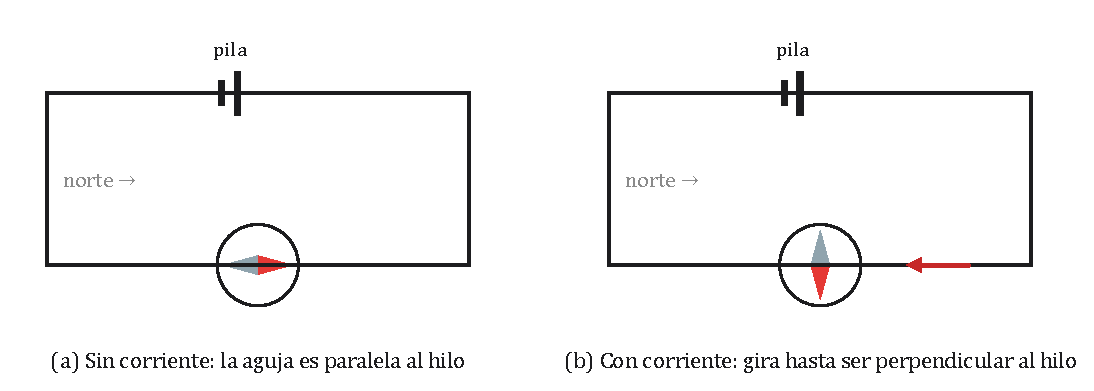
\includegraphics[width=0.9\linewidth]{images/UD6/oersted}
    \caption{Experiencia de Oersted vista desde arriba.}
    \label{fig:mag-oersted}
\end{figure}

\section{Fuerza sobre una carga en movimiento: ley de Lorentz}\label{sec:mag-lorentz}

Experimentalmente se observa que un campo magnético no ejerce fuerza sobre una carga en reposo, ni sobre una carga que se
mueve en la dirección del campo. En los demás casos la fuerza es perpendicular a la velocidad y al campo, y es máxima cuando la
carga se mueve perpendicularmente a las líneas de campo. Todo esto se resume en la \rojon{ley de Lorentz}:
\begin{centeredequation}
    \boxed{\vec F = q\,(\vec v\times\vec B)} \qquad\qquad F = |q|\,v\,B\sen\varphi \label{eq:mag-lorentz}
\end{centeredequation}
donde \(\varphi\) es el ángulo entre \(\vec v\) y \(\vec B\). El sentido de \(\vec v\times\vec B\) es el de avance de un
sacacorchos que gira llevando \(\vec v\) hacia \(\vec B\) por el camino más corto; para una carga negativa, la fuerza tiene el
sentido contrario (figura~\ref{fig:mag-lorentz}).

\begin{figure}[H]
    \centering
    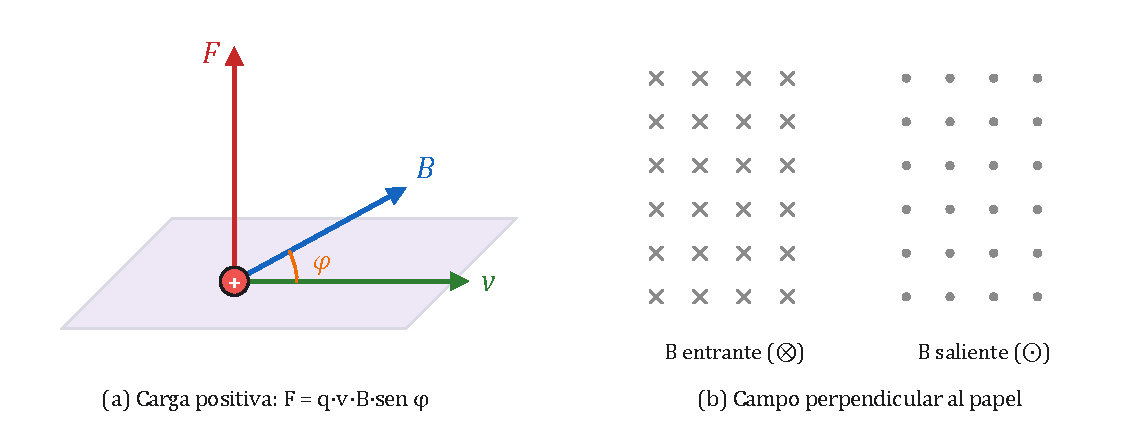
\includegraphics[width=0.9\linewidth]{images/UD6/lorentz}
    \caption{(a) La fuerza magnética es perpendicular al plano de \(\vec v\) y \(\vec B\). (b) Convenio para dibujar campos
    perpendiculares al papel: \(\times\) si entran y \(\bullet\) si salen.}
    \label{fig:mag-lorentz}
\end{figure}

\paragraph{Unidad.} La unidad de \(B\) en el SI es el \azuln{tesla} (\unit{\tesla}): el campo que ejerce una fuerza de
\qty{1}{\newton} sobre una carga de \qty{1}{\coulomb} que se mueve a \qty{1}{\m\per\second} perpendicularmente a él,
\(\qty{1}{\tesla} = \qty{1}{\newton\per\ampere\per\m}\). Es una unidad grande: el campo magnético terrestre es de unos
\qty{5e-5}{\tesla}, un imán de nevera crea unos \qty{0.01}{\tesla} y una resonancia magnética, entre \qty{1.5}{\tesla} y
\qty{3}{\tesla}.

\paragraph{Fuerza de Lorentz generalizada.} Si en una región hay a la vez un campo eléctrico y uno magnético:
\begin{centeredequation}
    \vec F = q\,\vec E + q\,(\vec v\times\vec B) = q\,(\vec E + \vec v\times\vec B) \label{eq:mag-lorentz-gen}
\end{centeredequation}

\begin{exercise}
    Una partícula con una carga de \qty{3}{\micro\coulomb} entra con una velocidad de \qty{2e6}{\m\per\second} en un campo
    magnético de \qty{2}{\tesla}, formando \ang{30} con él. ¿Qué fuerza actúa sobre ella?
    \begin{solu}
        \(F = q v B\sen\varphi = 3\cdot 10^{-6}\cdot 2\cdot 10^6\cdot 2\cdot\sen\ang{30} = \textcolor{red}{\qty{6}{\newton}}\),
        \textcolor{blue}{perpendicular al plano que forman \(\vec v\) y \(\vec B\).}
    \end{solu}
\end{exercise}

\begin{exercise}
    Un protón con una energía cinética de \qty{4}{\mega\electronvolt} se mueve perpendicularmente a un campo de \qty{1.2}{\tesla}.
    ¿Qué fuerza actúa sobre él? (\(m_p = \qty{1.67e-27}{\kg}\); \(\qty{1}{\electronvolt} = \qty{1.6e-19}{\joule}\)).
    \begin{solu}
        \(v = \sqrt{\dfrac{2E_c}{m}} = \sqrt{\dfrac{2\cdot 4\cdot 10^6\cdot 1{,}6\cdot 10^{-19}}{1{,}67\cdot 10^{-27}}} = \qty{2.77e7}{\m\per\second}\);
        \(F = q v B = \textcolor{red}{\qty{5.32e-12}{\newton}}\).
    \end{solu}
\end{exercise}

\begin{exercise}
    En una región hay un campo eléctrico \(\vec E = 2\,\vec{i} - 1000\,\vec{k}\ \unit{\newton\per\coulomb}\) y un campo magnético
    \(\vec B = 0{,}4\,\vec{i} + \vec{j}\ \unit{\tesla}\). Calcula la fuerza sobre una carga de \qty{5}{\micro\coulomb} que se mueve
    con \(\vec v = 2000\,\vec{i}\ \unit{\m\per\second}\).
    \begin{solu}
        \(\vec v\times\vec B = 2000\,\vec{i}\times(0{,}4\,\vec{i} + \vec{j}) = 2000\,\vec{k}\) \textcolor{blue}{(porque \(\vec{i}\times\vec{i} = 0\) y \(\vec{i}\times\vec{j} = \vec{k}\)).}
        \[ \vec F = q(\vec E + \vec v\times\vec B) = 5\cdot 10^{-6}\,(2\,\vec{i} + 1000\,\vec{k}) = \textcolor{red}{(1\cdot 10^{-5}\,\vec{i} + 5\cdot 10^{-3}\,\vec{k})\ \unit{\newton}} \]
    \end{solu}
\end{exercise}

\section{Movimiento de cargas en un campo magnético}\label{sec:mag-movimiento}

Como la fuerza magnética es siempre perpendicular a la velocidad, \textbf{no hace trabajo}: no cambia el módulo de la velocidad
ni la energía cinética de la partícula, solo su dirección.

\paragraph{Velocidad perpendicular al campo.} La fuerza actúa como fuerza centrípeta y la partícula describe una
\textbf{circunferencia} con movimiento uniforme (figura~\ref{fig:mag-circular}):
\begin{equation*}
    |q|\,v\,B = m\,\dfrac{v^2}{R} \qquad\Rightarrow\qquad \boxed{R = \dfrac{m\,v}{|q|\,B}}
\end{equation*}
El radio es proporcional a la cantidad de movimiento e inversamente proporcional a la carga y al campo. El período y la
frecuencia del movimiento (la \azuln{frecuencia ciclotrón}) no dependen de la velocidad ni del radio:
\begin{centeredequation}
    \omega = \dfrac{v}{R} = \dfrac{|q|\,B}{m} \qquad\qquad T = \dfrac{2\pi m}{|q|\,B} \qquad\qquad f = \dfrac{|q|\,B}{2\pi m} \label{eq:mag-ciclotron}
\end{centeredequation}
En esto se basan el \emph{ciclotrón} (un acelerador de partículas) y el \emph{espectrómetro de masas}, que separa los isótopos
de un elemento por el radio de su trayectoria.

\begin{figure}[H]
    \centering
    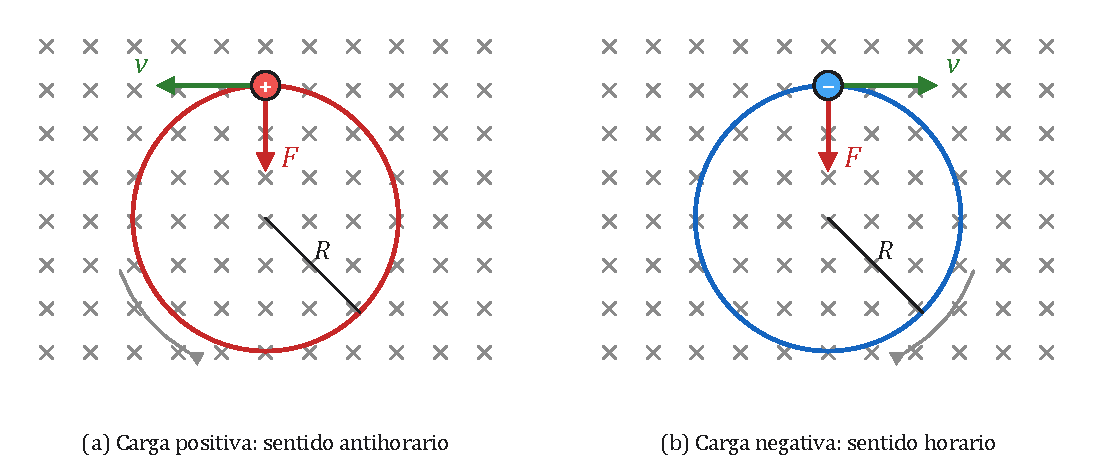
\includegraphics[width=0.9\linewidth]{images/UD6/circular}
    \caption{Trayectorias en un campo entrante: el sentido de giro depende del signo de la carga.}
    \label{fig:mag-circular}
\end{figure}

\paragraph{Velocidad oblicua.} Si la velocidad forma un ángulo con el campo, la componente paralela a \(\vec B\) no cambia y la
perpendicular produce un giro: la trayectoria es una \textbf{hélice} (figura~\ref{fig:mag-helice}). Así quedan atrapadas las
partículas del viento solar en el campo magnético terrestre; al llegar a la atmósfera cerca de los polos producen las auroras.

\begin{figure}[H]
    \centering
    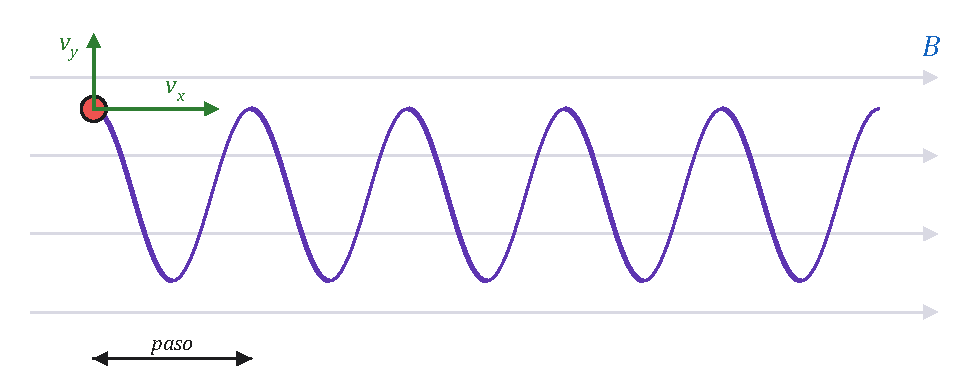
\includegraphics[width=0.66\linewidth]{images/UD6/helice}
    \caption{Trayectoria helicoidal de una carga cuya velocidad no es perpendicular al campo.}
    \label{fig:mag-helice}
\end{figure}

\begin{exercise}
    Un electrón con una velocidad de \qty{3000}{\km\per\second} entra perpendicularmente en un campo uniforme de
    \qty{2e-3}{\tesla}. Calcula el radio de su órbita y la frecuencia del movimiento (\(m_e = \qty{9.11e-31}{\kg}\)).
    \begin{solu}
        \(R = \dfrac{m v}{e B} = \dfrac{9{,}11\cdot 10^{-31}\cdot 3\cdot 10^6}{1{,}6\cdot 10^{-19}\cdot 2\cdot 10^{-3}} = \textcolor{red}{\qty{8.54e-3}{\m}}\);
        \(f = \dfrac{e B}{2\pi m} = \textcolor{red}{\qty{5.59e7}{\hertz}}\).
    \end{solu}
\end{exercise}

\begin{exercise}
    Un protón entra perpendicularmente en un campo de \qty{2}{\tesla}. ¿Con qué velocidad debe entrar para que el radio de su
    trayectoria sea de \qty{3}{\cm}?
    \begin{solu}
        \(v = \dfrac{q B R}{m} = \dfrac{1{,}6\cdot 10^{-19}\cdot 2\cdot 0{,}03}{1{,}67\cdot 10^{-27}} = \textcolor{red}{\qty{5.75e6}{\m\per\second}}\).
    \end{solu}
\end{exercise}

\section{Fuerza sobre una corriente: ley de Laplace}\label{sec:mag-laplace}

Una corriente es un conjunto de cargas en movimiento, así que un campo magnético ejerce fuerza sobre un conductor por el que
circula corriente. Si el conductor tiene \(n\) portadores de carga \(q\) por unidad de volumen, sección \(S\) y longitud \(L\), y
los portadores se mueven con velocidad \(\vec v\), la intensidad es \(I = nqSv\) y la fuerza total es
\(\vec F = nSL\,q\,(\vec v\times\vec B)\). Definiendo un vector \(\vec L\) de módulo la longitud del conductor y con el sentido de
la corriente, queda la \rojon{ley de Laplace}:
\begin{centeredequation}
    \boxed{\vec F = I\,(\vec L\times\vec B)} \qquad\qquad F = I\,L\,B\sen\alpha \label{eq:mag-laplace}
\end{centeredequation}
donde \(\alpha\) es el ángulo entre el conductor y el campo (figura~\ref{fig:mag-laplace}).

\begin{figure}[H]
    \centering
    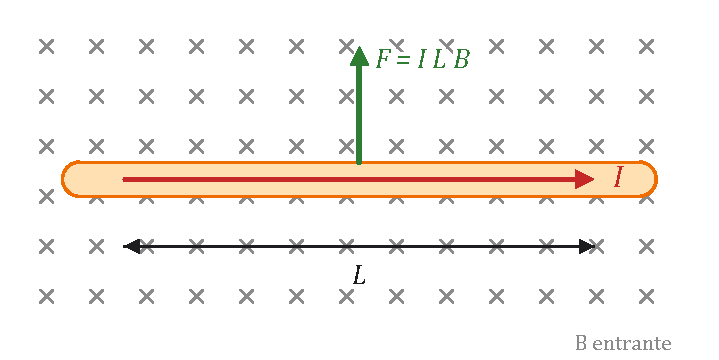
\includegraphics[width=0.55\linewidth]{images/UD6/laplace}
    \caption{Fuerza sobre un conductor perpendicular a un campo entrante.}
    \label{fig:mag-laplace}
\end{figure}

\begin{exercise}
    Un conductor de \qty{50}{\cm} por el que circula una corriente de \qty{0.4}{\ampere} está en un campo uniforme de
    \qty{0.5}{\tesla} y forma \ang{30} con él. ¿Qué fuerza actúa sobre él?
    \begin{solu}
        \(F = I L B\sen\alpha = 0{,}4\cdot 0{,}5\cdot 0{,}5\cdot\sen\ang{30} = \textcolor{red}{\qty{0.05}{\newton}}\).
    \end{solu}
\end{exercise}

\begin{exercise}
    Un conductor de \qty{20}{\cm} está sobre el eje \(Y\) y lleva una corriente de \qty{3}{\ampere} en sentido positivo. Si el
    campo es \(\vec B = 0{,}1\,\vec{i} - 0{,}2\,\vec{j} + 0{,}4\,\vec{k}\ \unit{\tesla}\), ¿qué fuerza actúa sobre él?
    \begin{solu}
        \(\vec L = 0{,}2\,\vec{j}\ \unit{\m}\).
        \(\vec L\times\vec B = 0{,}2\,\vec{j}\times(0{,}1\,\vec{i} - 0{,}2\,\vec{j} + 0{,}4\,\vec{k}) = 0{,}2\,(-0{,}1\,\vec{k} + 0{,}4\,\vec{i})\).
        \[ \vec F = I\,(\vec L\times\vec B) = \textcolor{red}{0{,}24\,\vec{i} - 0{,}06\,\vec{k}\ \unit{\newton}} \]
    \end{solu}
\end{exercise}

\subsection{Momento sobre una espira. El motor eléctrico}\label{subsec:mag-espira}

Sobre una espira rectangular de lados \(a\) y \(b\) por la que circula \(I\), en un campo uniforme, las fuerzas sobre los lados
opuestos son iguales y de sentidos contrarios. La fuerza neta es nula, pero las fuerzas sobre los dos lados perpendiculares al
campo no están en la misma recta: forman un \textbf{par de fuerzas} que hace girar la espira (figura~\ref{fig:mag-espira}). Cada
una vale \(F = I\,a\,B\) y su brazo es \(b\sen\alpha\), donde \(\alpha\) es el ángulo entre \(\vec B\) y el vector superficie
\(\vec S\) (perpendicular a la espira, con el sentido que da la regla de la mano derecha aplicada a la corriente):
\begin{centeredequation}
    M = I\,a\,B\,b\sen\alpha = I\,S\,B\sen\alpha \qquad\Rightarrow\qquad \boxed{\vec M = I\,(\vec S\times\vec B) = \vec m\times\vec B} \label{eq:mag-par}
\end{centeredequation}
El vector \(\vec m = I\vec S\) es el \azuln{momento magnético} de la espira; para una bobina de \(N\) espiras, \(\vec m = N I\vec S\).
El par tiende a girar la espira hasta que \(\vec m\) se alinea con \(\vec B\), igual que una brújula. Es el principio del
\textbf{motor eléctrico} y de los galvanómetros: si cada media vuelta se invierte el sentido de la corriente (con un colector de
delgas), el par siempre hace girar la espira en el mismo sentido.

\begin{figure}[H]
    \centering
    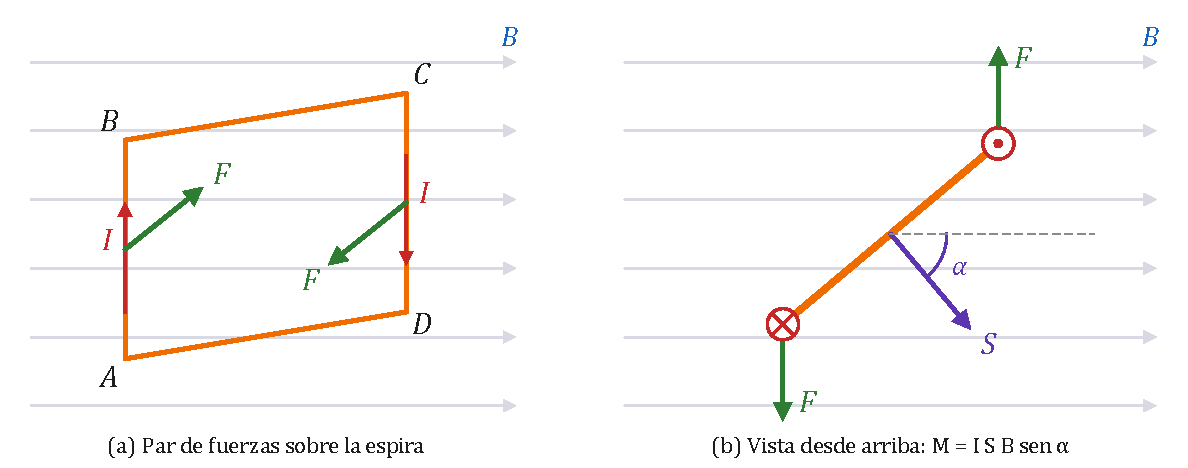
\includegraphics[width=0.95\linewidth]{images/UD6/espira_par}
    \caption{Par de fuerzas sobre una espira con corriente en un campo uniforme.}
    \label{fig:mag-espira}
\end{figure}

\begin{exercise}
    Una espira circular de \qty{12}{\cm} de diámetro, recorrida por \qty{3}{\ampere}, está en un campo de \qty{0.5}{\tesla}. Calcula
    su momento magnético y el momento del par cuando su vector superficie forma \ang{60} con el campo. ¿Cuál es el momento máximo?
    \begin{solu}
        \(S = \pi\cdot 0{,}06^2 = \qty{1.13e-2}{\m\squared}\); \(m = IS = \textcolor{red}{\qty{3.39e-2}{\ampere\m\squared}}\).

        \(M = m B\sen\ang{60} = \textcolor{red}{\qty{1.47e-2}{\newton\m}}\); \(M_{\text{máx}} = m B = \textcolor{red}{\qty{1.70e-2}{\newton\m}}\) \textcolor{blue}{(con la espira paralela al campo).}
    \end{solu}
\end{exercise}

\section{Campos magnéticos creados por corrientes}\label{sec:mag-creados}

\subsection{Campo de una carga en movimiento. Ley de Biot y Savart}\label{subsec:mag-biot}

Una carga \(q\) que se mueve con velocidad \(\vec v\) crea en un punto situado en la posición \(\vec r\) un campo:
\begin{centeredequation}
    \vec B = \dfrac{\mu_0}{4\pi}\,\dfrac{q\,\vec v\times\vec u_r}{r^2} \qquad\qquad B = \dfrac{\mu_0}{4\pi}\,\dfrac{q\,v\sen\varphi}{r^2} \label{eq:mag-carga}
\end{centeredequation}
donde \(\mu_0 = 4\pi\cdot 10^{-7}\ \unit{\tesla\m\per\ampere}\) es la \azuln{permeabilidad magnética del vacío}. Del mismo modo, un
elemento de corriente \(I\,d\vec l\) crea un campo elemental (\rojon{ley de Biot y Savart}):
\begin{centeredequation}
    d\vec B = \dfrac{\mu_0}{4\pi}\,\dfrac{I\,d\vec l\times\vec u_r}{r^2} \label{eq:mag-biot}
\end{centeredequation}
El campo de cualquier conductor se obtiene sumando (integrando) los campos de todos sus elementos.

\begin{exercise}
    En el modelo de Bohr del átomo de hidrógeno, el electrón gira alrededor del protón a \qty{5.29e-11}{\m} con una velocidad de
    \qty{2.19e6}{\m\per\second}. ¿Qué campo magnético crea en la posición del protón?
    \begin{solu}
        \textcolor{blue}{\(\vec v\) es perpendicular a \(\vec r\):}
        \(B = 10^{-7}\,\dfrac{1{,}6\cdot 10^{-19}\cdot 2{,}19\cdot 10^6}{(5{,}29\cdot 10^{-11})^2} = \textcolor{red}{\qty{12.5}{\tesla}}\):
        \textcolor{blue}{un campo enorme, a escala atómica.}
    \end{solu}
\end{exercise}

\subsection{Corriente rectilínea indefinida}\label{subsec:mag-hilo}

Integrando la ley de Biot y Savart a lo largo de un hilo infinito, a una distancia \(r\) de él:
\begin{centeredequation}
    \boxed{B = \dfrac{\mu_0\,I}{2\pi\,r}} \label{eq:mag-hilo}
\end{centeredequation}
Las líneas de campo son \textbf{circunferencias concéntricas} con el hilo, en planos perpendiculares a él. Su sentido lo da la
\azuln{regla de la mano derecha}: con el pulgar en el sentido de la corriente, los demás dedos se cierran en el sentido del campo
(figura~\ref{fig:mag-hilo}).

\begin{figure}[H]
    \centering
    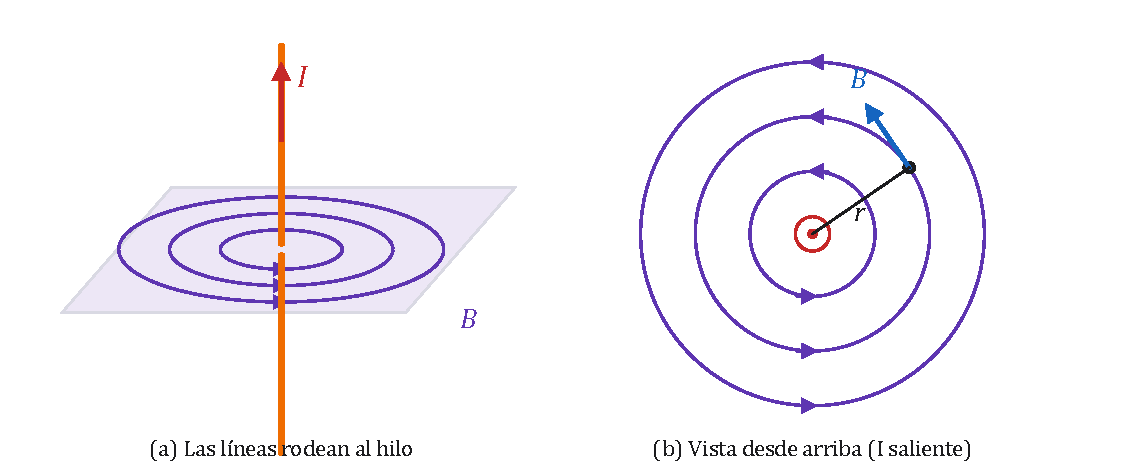
\includegraphics[width=0.92\linewidth]{images/UD6/hilo}
    \caption{Campo de una corriente rectilínea. \(\vec B\) es tangente a las circunferencias.}
    \label{fig:mag-hilo}
\end{figure}

\begin{exercise}
    Dos conductores perpendiculares al papel, separados \qty{30}{\cm}, llevan corrientes de \qty{6}{\ampere} y \qty{10}{\ampere}
    entrantes. Calcula el campo en el punto medio. ¿En qué punto de la recta que los une se anula?
    \begin{solu}
        \textcolor{blue}{En el punto medio los dos campos tienen sentidos opuestos:}
        \(B = \dfrac{\mu_0}{2\pi}\,\dfrac{10 - 6}{0{,}15} = \textcolor{red}{\qty{5.33e-6}{\tesla}}\), \textcolor{blue}{en el sentido del creado por el de \qty{10}{\ampere}.}

        \textcolor{blue}{Se anula entre ellos, a una distancia \(x\) del de \qty{6}{\ampere}:} \(\dfrac{6}{x} = \dfrac{10}{0{,}3 - x} \Rightarrow \textcolor{red}{x = \qty{11.25}{\cm}}\).
    \end{solu}
\end{exercise}

\subsection{Espira circular}\label{subsec:mag-espira-circular}

En el centro de una espira de radio \(R\), todos los elementos de corriente son perpendiculares al radio y están a la misma
distancia, así que sus campos se suman directamente:
\begin{centeredequation}
    B = \dfrac{\mu_0 I}{4\pi R^2}\oint dl = \dfrac{\mu_0 I}{4\pi R^2}\,2\pi R \qquad\Rightarrow\qquad \boxed{B = \dfrac{\mu_0\,I}{2R}} \label{eq:mag-espira}
\end{centeredequation}
El campo es perpendicular al plano de la espira, con el sentido que da la regla de la mano derecha (figura~\ref{fig:mag-espira-campo}).
Para una bobina plana de \(N\) espiras, \(B = N\mu_0 I/2R\). Una espira se comporta como un imán: la cara por la que salen las
líneas es un polo norte.

\begin{figure}[H]
    \centering
    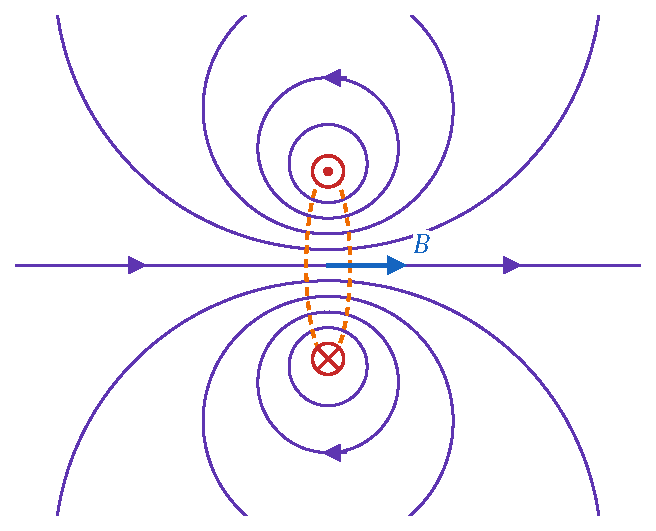
\includegraphics[width=0.45\linewidth]{images/UD6/espira_campo}
    \caption{Líneas del campo de una espira circular en un corte por su eje.}
    \label{fig:mag-espira-campo}
\end{figure}

\begin{exercise}
    ¿Qué radio tiene una espira por la que circulan \qty{4}{\ampere} si el campo en su centro es de \qty{2e-5}{\tesla}?
    \begin{solu}
        \(R = \dfrac{\mu_0 I}{2B} = \dfrac{4\pi\cdot 10^{-7}\cdot 4}{2\cdot 2\cdot 10^{-5}} = \textcolor{red}{\qty{0.126}{\m}}\).
    \end{solu}
\end{exercise}

\subsection{Ley de Ampère}\label{subsec:mag-ampere}

En los campos gravitatorio y eléctrico la \emph{circulación} del campo a lo largo de una línea cerrada es nula: son campos
conservativos. Para el campo magnético no ocurre lo mismo. Calculemos la circulación a lo largo de una circunferencia de
radio \(r\) centrada en un hilo: \(\vec B\) y \(d\vec l\) son paralelos y \(B\) es constante,
\begin{equation*}
    \oint\vec B\cdot d\vec l = B\oint dl = \dfrac{\mu_0 I}{2\pi r}\,2\pi r = \mu_0 I
\end{equation*}

\begin{definition}[Ley de Ampère]
    La circulación del campo magnético a lo largo de cualquier línea cerrada es igual a \(\mu_0\) por la intensidad neta que
    atraviesa la superficie limitada por esa línea:
    \begin{centeredequation}
        \boxed{\oint\vec B\cdot d\vec l = \mu_0\sum I} \label{eq:mag-ampere}
    \end{centeredequation}
    Se cuentan como positivas las corrientes cuyo sentido coincide con el que da la regla de la mano derecha al recorrer la línea.
\end{definition}

Como la circulación no es nula, \textbf{el campo magnético no es conservativo}: no se puede definir un potencial magnético como
en los otros campos.

\paragraph{Campo de un solenoide.} Un \rojon{solenoide} es un conjunto de espiras iguales enrolladas en hélice, con una longitud
\(L\) mucho mayor que su radio. Dentro, el campo es prácticamente uniforme y paralelo al eje; fuera, casi nulo (salvo cerca de
los extremos, donde se parece al de un imán de barra). Aplicando la ley de Ampère al rectángulo \(ACDE\) de la
figura~\ref{fig:mag-solenoide}: en los lados \(CD\) y \(EA\) el campo es perpendicular al camino; en \(DE\), fuera, es nulo; solo
contribuye el lado \(AC\), de longitud \(l\), por dentro. Si hay \(n = N/L\) espiras por unidad de longitud, el rectángulo encierra
\(n\,l\) espiras:
\begin{equation*}
    B\,l = \mu_0\,n\,l\,I \qquad\Rightarrow\qquad \boxed{B = \mu_0\,\dfrac{N}{L}\,I = \mu_0\,n\,I}
\end{equation*}

\begin{figure}[H]
    \centering
    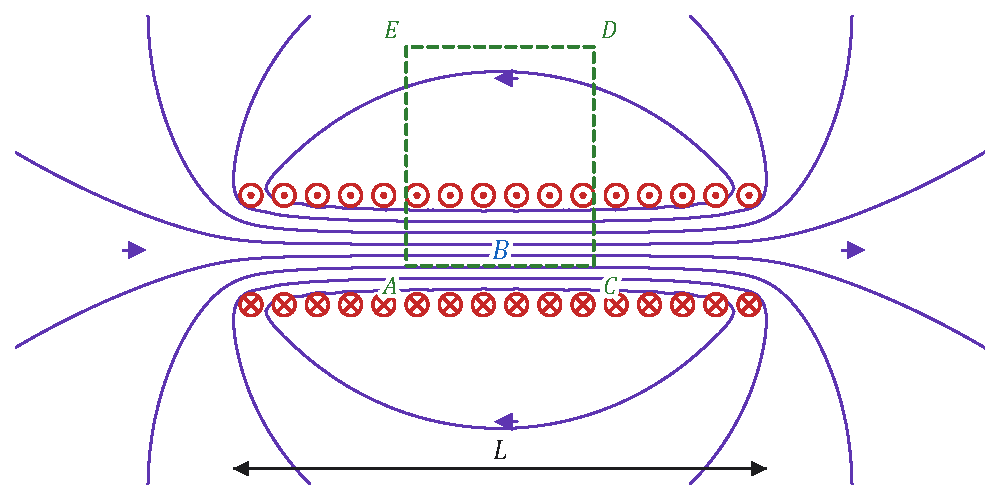
\includegraphics[width=0.75\linewidth]{images/UD6/solenoide}
    \caption{Corte de un solenoide (líneas de campo calculadas) y camino rectangular para aplicar la ley de Ampère.}
    \label{fig:mag-solenoide}
\end{figure}

Si el solenoide se enrolla sobre un núcleo de hierro, el campo se multiplica cientos de veces: es un \textbf{electroimán}.

\begin{exercise}
    ¿Qué longitud debe tener un solenoide de 800 espiras, por el que circulan \qty{1.5}{\ampere}, para que el campo en su interior
    sea de \qty{6e-3}{\tesla}?
    \begin{solu}
        \(L = \dfrac{\mu_0 N I}{B} = \dfrac{4\pi\cdot 10^{-7}\cdot 800\cdot 1{,}5}{6\cdot 10^{-3}} = \textcolor{red}{\qty{0.251}{\m}}\).
    \end{solu}
\end{exercise}

\subsection{Fuerzas entre corrientes paralelas}\label{subsec:mag-paralelas}

Dos conductores rectilíneos y paralelos, separados \(d\), se ejercen fuerzas: el campo que crea el primero en la posición del
segundo, \(B_1 = \mu_0 I_1/2\pi d\), actúa sobre la corriente \(I_2\) según la ley de Laplace, y al revés:
\begin{centeredequation}
    \boxed{\dfrac{F}{L} = \dfrac{\mu_0\,I_1\,I_2}{2\pi\,d}} \label{eq:mag-paralelas}
\end{centeredequation}
\textbf{Las corrientes del mismo sentido se atraen y las de sentidos opuestos se repelen} (figura~\ref{fig:mag-paralelas}): justo
al revés que las cargas.

\begin{figure}[H]
    \centering
    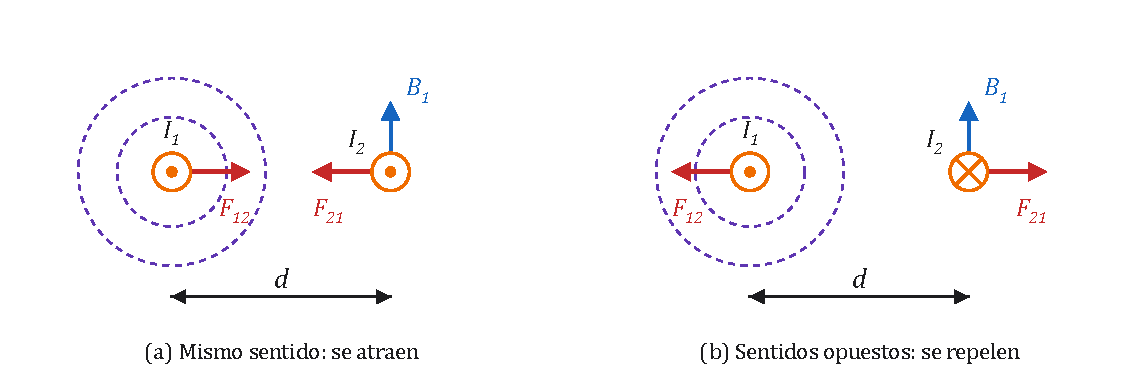
\includegraphics[width=0.9\linewidth]{images/UD6/paralelas}
    \caption{Fuerzas entre dos corrientes paralelas, vistas en corte.}
    \label{fig:mag-paralelas}
\end{figure}

\begin{remark}
    Esta fuerza sirvió para definir el \textbf{amperio}: la corriente que, circulando por dos conductores paralelos, rectilíneos e
    indefinidos, separados \qty{1}{\m} en el vacío, hace que se atraigan con una fuerza de \qty{2e-7}{\newton} por metro. (Desde
    2019 el amperio se define a partir del valor fijo de la carga del electrón, pero la relación sigue siendo válida.)
\end{remark}

\begin{exercise}
    Dos hilos paralelos de \qty{30}{\cm} están separados \qty{20}{\cm} y llevan \qty{40}{\ampere} cada uno en el mismo sentido.
    ¿Qué fuerza se ejercen?
    \begin{solu}
        \(F = \dfrac{\mu_0 I_1 I_2 L}{2\pi d} = 2\cdot 10^{-7}\,\dfrac{40\cdot 40\cdot 0{,}3}{0{,}2} = \textcolor{red}{\qty{4.8e-4}{\newton}}\), \textcolor{red}{de atracción}.
    \end{solu}
\end{exercise}

\section{Inducción electromagnética}\label{sec:mag-induccion}

\subsection{Flujo magnético}\label{subsec:mag-flujo}

El \rojon{flujo magnético} a través de una superficie mide el número de líneas de campo que la atraviesan. Para un campo
uniforme y una superficie plana:
\begin{centeredequation}
    \boxed{\Phi = \vec B\cdot\vec S = B\,S\cos\alpha} \label{eq:mag-flujo}
\end{centeredequation}
donde \(\alpha\) es el ángulo entre \(\vec B\) y el vector superficie. En general, \(\Phi = \int\vec B\cdot d\vec S\). Su unidad es
el \azuln{weber}: \(\qty{1}{\weber} = \qty{1}{\tesla\m\squared}\). Como las líneas del campo magnético son cerradas, todas las que
entran en una superficie cerrada salen de ella: \textbf{el flujo magnético a través de una superficie cerrada es siempre nulo}
(no hay polos magnéticos aislados).

\begin{exercise}
    Calcula el flujo magnético a través de una espira cuadrada de \qty{10}{\cm} de lado perpendicular a un campo de
    \qty{0.8}{\tesla}, y a través de una espira circular de \qty{30}{\cm} de diámetro cuyo eje forma \ang{60} con un campo de
    \qty{0.5}{\tesla}.
    \begin{solu}
        \(\Phi_1 = B S = 0{,}8\cdot 0{,}01 = \textcolor{red}{\qty{8e-3}{\weber}}\);
        \(\Phi_2 = B S\cos\ang{60} = 0{,}5\cdot\pi\cdot 0{,}15^2\cdot 0{,}5 = \textcolor{red}{\qty{1.77e-2}{\weber}}\).
    \end{solu}
\end{exercise}

\subsection{Experiencias de Faraday y Henry}\label{subsec:mag-faraday}

Faraday conectó una bobina a un galvanómetro (un amperímetro muy sensible) y observó (figura~\ref{fig:mag-faraday}):
\begin{itemize}
    \item al acercar un imán, el galvanómetro marca corriente, y más cuanto más deprisa se mueve el imán;
    \item si el imán se para, la corriente cesa;
    \item al alejarlo, la corriente circula en sentido contrario; lo mismo ocurre si se acerca el otro polo;
    \item se obtiene lo mismo dejando quieto el imán y moviendo la bobina, o cambiando la corriente de otra bobina cercana.
\end{itemize}
A la corriente que aparece se le llama \azuln{corriente inducida}, y a la fuerza electromotriz que la produce, \azuln{fem inducida}.
El circuito donde aparece es el \emph{inducido} y el agente que la produce (el imán), el \emph{inductor}.

\begin{figure}[H]
    \centering
    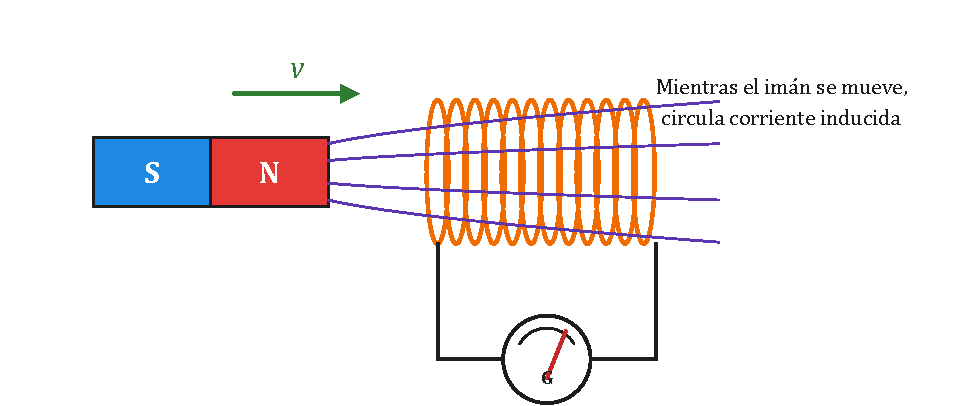
\includegraphics[width=0.7\linewidth]{images/UD6/faraday}
    \caption{Experiencia de Faraday.}
    \label{fig:mag-faraday}
\end{figure}

Henry, por su parte, observó que un conductor que se mueve cortando las líneas de un campo magnético tiene una diferencia de
potencial entre sus extremos. Sobre los electrones del conductor actúa la fuerza de Lorentz, que los acumula en un extremo. Si una
varilla de longitud \(l\) se mueve con velocidad \(v\) perpendicular a \(B\) (figura~\ref{fig:mag-varilla}), el trabajo por unidad
de carga a lo largo de la varilla es la fem:
\begin{centeredequation}
    \varepsilon = \dfrac{F\,l}{q} = \dfrac{q\,v\,B\,l}{q} \qquad\Rightarrow\qquad \boxed{\varepsilon = B\,l\,v} \label{eq:mag-Blv}
\end{centeredequation}
Si la varilla cierra un circuito, circula corriente; entonces el campo ejerce sobre la varilla una fuerza (ley de Laplace) que se
opone al movimiento, y hay que empujarla para mantener la velocidad: así se transforma energía mecánica en eléctrica.

\begin{figure}[H]
    \centering
    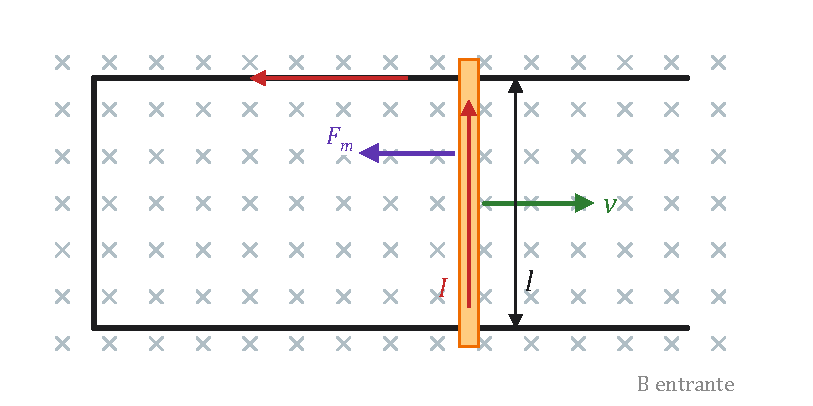
\includegraphics[width=0.6\linewidth]{images/UD6/varilla}
    \caption{Varilla que se desliza sobre unos raíles en un campo entrante.}
    \label{fig:mag-varilla}
\end{figure}

\subsection{Ley de Faraday-Lenz}\label{subsec:mag-faraday-lenz}

Todas estas experiencias tienen algo en común: \textbf{varía el flujo magnético} a través del circuito (por moverse el imán,
cambiar el área o la orientación del circuito, o cambiar el campo).

\begin{definition}[Ley de Faraday-Lenz]
    La fem inducida en un circuito es igual a la rapidez con que varía el flujo magnético que lo atraviesa, cambiada de signo.
    Para una bobina de \(N\) espiras:
    \begin{centeredequation}
        \boxed{\varepsilon = -N\,\dfrac{d\Phi}{dt}} \qquad\qquad \varepsilon_{\text{media}} = -N\,\dfrac{\Delta\Phi}{\Delta t} \label{eq:mag-faraday}
    \end{centeredequation}
\end{definition}

El signo menos expresa la \rojon{ley de Lenz}: \emph{la corriente inducida circula en el sentido en que su propio campo magnético
se opone a la variación del flujo que la produce}. Si el flujo aumenta, el campo inducido es contrario al inductor; si disminuye,
tiene su mismo sentido. Es una consecuencia de la conservación de la energía: si la corriente inducida favoreciera el cambio, se
crearía energía de la nada.

\begin{figure}[H]
    \centering
    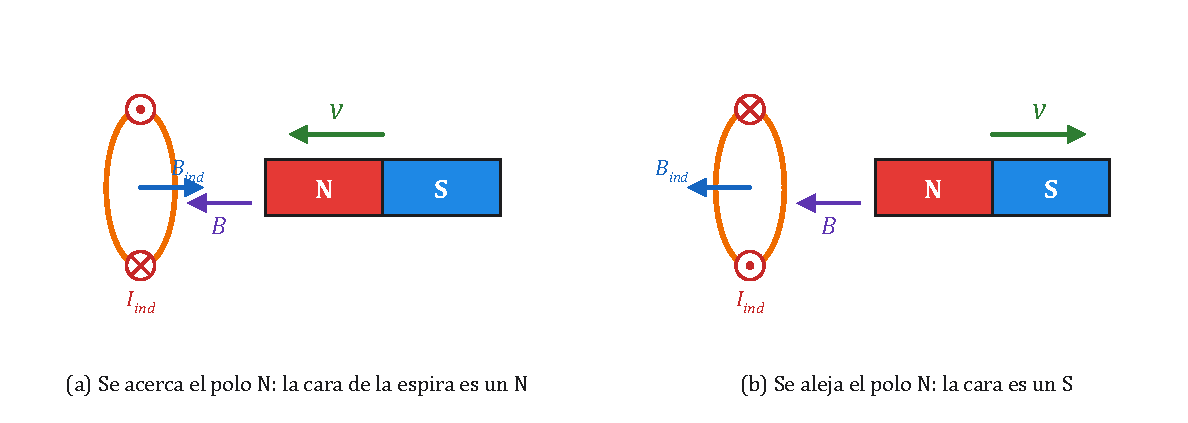
\includegraphics[width=0.95\linewidth]{images/UD6/lenz}
    \caption{Ley de Lenz. (a) Al acercar el polo norte, la espira crea un polo norte enfrente que lo repele. (b) Al alejarlo,
    crea un polo sur que lo atrae. En los dos casos la espira se opone al movimiento del imán.}
    \label{fig:mag-lenz}
\end{figure}

Con la varilla de la figura~\ref{fig:mag-varilla} se comprueba que las dos leyes coinciden: el área del circuito aumenta
\(dS = l\,v\,dt\), el flujo aumenta \(d\Phi = B\,l\,v\,dt\) y \(|\varepsilon| = d\Phi/dt = Blv\). Como el flujo entrante aumenta, la
corriente circula en sentido antihorario, creando un campo saliente.

\begin{exercise}
    Una bobina de 400 espiras cuadradas de \qty{5}{\cm} de lado está perpendicular a un campo que pasa de \qty{0.3}{\tesla} a
    \qty{0.8}{\tesla} en \qty{0.02}{\second}. ¿Qué fem media se induce?
    \begin{solu}
        \(|\varepsilon| = N S\,\dfrac{\Delta B}{\Delta t} = 400\cdot 0{,}0025\cdot\dfrac{0{,}5}{0{,}02} = \textcolor{red}{\qty{25}{\volt}}\).
    \end{solu}
\end{exercise}

\begin{exercise}
    Una varilla de \qty{40}{\cm} se mueve a \qty{5}{\m\per\second} sobre unos raíles, perpendicular a un campo de \qty{0.3}{\tesla}.
    Calcula la fem inducida y, si la resistencia del circuito es de \qty{2}{\ohm}, la intensidad y la fuerza que hay que hacer para
    mantener la velocidad.
    \begin{solu}
        \(\varepsilon = Blv = 0{,}3\cdot 0{,}4\cdot 5 = \textcolor{red}{\qty{0.6}{\volt}}\); \(I = \dfrac{\varepsilon}{R} = \textcolor{red}{\qty{0.3}{\ampere}}\);
        \(F = I l B = 0{,}3\cdot 0{,}4\cdot 0{,}3 = \textcolor{red}{\qty{0.036}{\newton}}\) \textcolor{blue}{(igual a la fuerza magnética que lo frena).}
    \end{solu}
\end{exercise}

\section{Aplicaciones de la inducción}\label{sec:mag-aplicaciones}

\subsection{El alternador}\label{subsec:mag-alternador}

Una bobina de \(N\) espiras de área \(S\) gira con velocidad angular constante \(\omega\) en un campo uniforme \(B\)
(figura~\ref{fig:mag-alternador}). El ángulo entre \(\vec B\) y \(\vec S\) es \(\alpha = \omega t\), y el flujo,
\(\Phi = B S\cos\omega t\). Por la ley de Faraday:
\begin{centeredequation}
    \varepsilon = -N\,\dfrac{d\Phi}{dt} = N B S\omega\sen\omega t \qquad\Rightarrow\qquad \boxed{\varepsilon = \varepsilon_0\sen\omega t,\quad \varepsilon_0 = N B S\omega} \label{eq:mag-alternador}
\end{centeredequation}
La fem es sinusoidal y la corriente cambia de sentido periódicamente: es una \textbf{corriente alterna}. Los extremos de la bobina
se conectan a unos anillos colectores sobre los que rozan unas escobillas, que llevan la corriente al circuito exterior. Si en
lugar de dos anillos se usa un anillo partido en dos mitades (conmutador), la corriente sale siempre en el mismo sentido: es una
\emph{dinamo}. El alternador transforma energía mecánica en eléctrica; el motor hace lo contrario.

\begin{figure}[H]
    \centering
    \begin{minipage}[b]{0.52\linewidth}
        \centering
        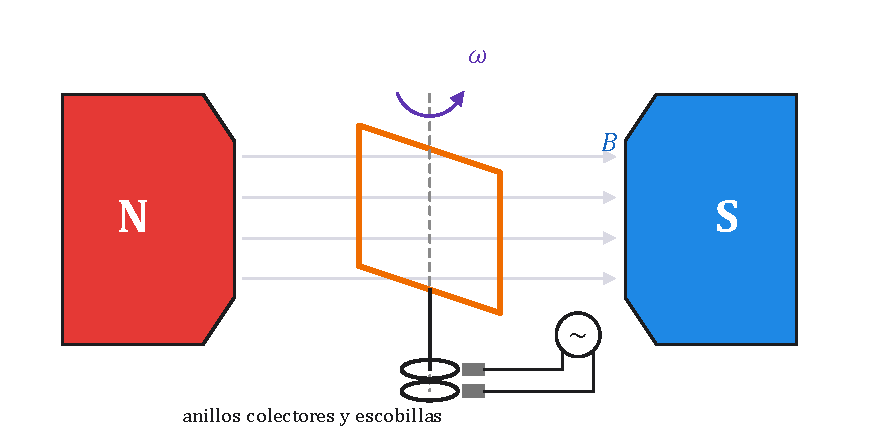
\includegraphics[width=\linewidth]{images/UD6/alternador}
    \end{minipage}\hfill
    \begin{minipage}[b]{0.44\linewidth}
        \centering
        \begin{tikzpicture}
            \begin{axis}[fisica, width=\linewidth, height=4.4cm, xmin=0, xmax=2.3, ymin=-1.35, ymax=1.45,
                xlabel={\(t\)}, ylabel={\(\varepsilon\)}, xtick={0.5,1,1.5,2}, xticklabels={\(\frac{T}{4}\),\(\frac{T}{2}\),\(\frac{3T}{4}\),\(T\)},
                ytick={-1,1}, yticklabels={\(-\varepsilon_0\),\(\varepsilon_0\)}]
                \addplot[domain=0:2.15, very thick, ocre, samples=120] {sin(deg(pi*x))};
            \end{axis}
        \end{tikzpicture}
    \end{minipage}
    \caption{Alternador y fem alterna que produce.}
    \label{fig:mag-alternador}
\end{figure}

\begin{exercise}
    Un alternador tiene una bobina de 200 espiras de \qty{100}{\cm\squared} que gira a \qty{50}{\hertz} en un campo de
    \qty{0.4}{\tesla}. ¿Cuál es la fem máxima? Escribe la expresión de la fem en función del tiempo.
    \begin{solu}
        \(\omega = 2\pi\cdot 50 = 100\pi\ \unit{\radian\per\second}\); \(\varepsilon_0 = N B S\omega = 200\cdot 0{,}4\cdot 0{,}01\cdot 100\pi = \textcolor{red}{\qty{251}{\volt}}\).
        \[ \textcolor{red}{\varepsilon = 251\sen(100\pi t)\ \text{(V)}} \]
    \end{solu}
\end{exercise}

\subsection{El transformador}\label{subsec:mag-transformador}

Un \rojon{transformador} cambia la tensión de una corriente alterna. Tiene dos bobinas enrolladas en un mismo núcleo de hierro: el
\emph{primario}, de \(N_1\) espiras, conectado a la tensión alterna \(V_1\), y el \emph{secundario}, de \(N_2\) espiras
(figura~\ref{fig:mag-transformador}). El núcleo conduce el flujo variable del primario hasta el secundario, de modo que el flujo
por espira es el mismo en las dos. Por la ley de Faraday:
\begin{equation*}
    V_1 = -N_1\,\dfrac{d\Phi}{dt} \qquad V_2 = -N_2\,\dfrac{d\Phi}{dt} \qquad\Rightarrow\qquad \boxed{\dfrac{V_2}{V_1} = \dfrac{N_2}{N_1}}
\end{equation*}
Si \(N_2 > N_1\) el transformador es \emph{elevador}; si \(N_2 < N_1\), \emph{reductor}. En un transformador ideal la potencia se
conserva, \(V_1 I_1 = V_2 I_2\), así que las intensidades están en razón inversa a las tensiones: \(I_2/I_1 = N_1/N_2\).

\begin{figure}[H]
    \centering
    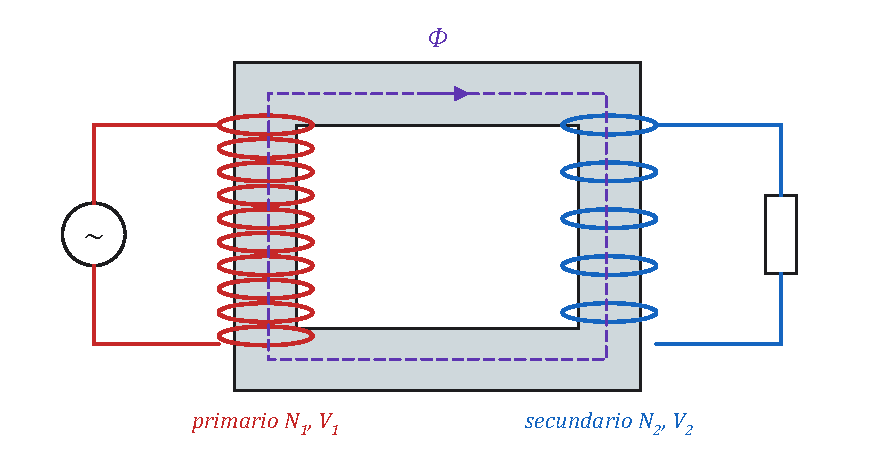
\includegraphics[width=0.6\linewidth]{images/UD6/transformador}
    \caption{Transformador reductor.}
    \label{fig:mag-transformador}
\end{figure}

\begin{remark}
    La energía eléctrica se transporta a muy alta tensión (cientos de miles de voltios) porque, para la misma potencia, la
    intensidad es menor y se pierde menos energía por efecto Joule en los cables (\(P_{\text{perdida}} = I^2 R\)). Junto a las
    centrales hay transformadores elevadores, y cerca de las ciudades, reductores. Los transformadores solo funcionan con corriente
    alterna: con corriente continua el flujo no varía.
\end{remark}

\begin{exercise}
    Un transformador tiene 1100 espiras en el primario, conectado a \qty{220}{\volt}, y 60 en el secundario. ¿Qué tensión da? Si
    por el secundario circulan \qty{2}{\ampere}, ¿qué intensidad circula por el primario?
    \begin{solu}
        \(V_2 = V_1\,\dfrac{N_2}{N_1} = \textcolor{red}{\qty{12}{\volt}}\); \(I_1 = I_2\,\dfrac{V_2}{V_1} = \textcolor{red}{\qty{0.109}{\ampere}}\).
    \end{solu}
\end{exercise}

\section{Resumen de fórmulas}\label{sec:mag-resumen}

\begin{table}[H]
    \centering
    \caption{Fórmulas principales del campo magnético y la inducción}
    \vspace{-5pt}
    \begin{tabular}{@{}lL{10cm}@{}}
        \toprule
        \textbf{Magnitud} & \textbf{Expresión} \\
        \midrule
        Ley de Lorentz & \(\vec F = q(\vec v\times\vec B)\), \quad \(F = |q| v B\sen\varphi\); \quad con \(\vec E\): \(\vec F = q(\vec E + \vec v\times\vec B)\) \\[3pt]
        Movimiento circular & \(R = m v/(|q| B)\), \quad \(T = 2\pi m/(|q| B)\) \\[3pt]
        Ley de Laplace & \(\vec F = I(\vec L\times\vec B)\), \quad \(F = I L B\sen\alpha\) \\[3pt]
        Espira en un campo & \(\vec M = \vec m\times\vec B\), \quad \(\vec m = N I\vec S\) \\[3pt]
        Hilo, espira, solenoide & \(B = \mu_0 I/(2\pi r)\); \quad \(B = \mu_0 I/(2R)\); \quad \(B = \mu_0 N I/L\) \\[3pt]
        Ley de Ampère & \(\oint\vec B\cdot d\vec l = \mu_0\sum I\), \quad \(\mu_0 = 4\pi\cdot 10^{-7}\ \unit{\tesla\m\per\ampere}\) \\[3pt]
        Corrientes paralelas & \(F/L = \mu_0 I_1 I_2/(2\pi d)\) \\[3pt]
        Flujo magnético & \(\Phi = \vec B\cdot\vec S = B S\cos\alpha\) \quad (\unit{\weber}) \\[3pt]
        Faraday-Lenz & \(\varepsilon = -N\,d\Phi/dt\); \quad varilla: \(\varepsilon = B l v\) \\[3pt]
        Alternador & \(\varepsilon = N B S\omega\sen\omega t\) \\[3pt]
        Transformador & \(V_2/V_1 = N_2/N_1 = I_1/I_2\) \\
        \bottomrule
    \end{tabular}
    \label{tab:mag-resumen}
\end{table}

\section{Prácticas de laboratorio}\label{sec:mag-practicas}

\subsection{Práctica 1: inducción electromagnética}\label{subsec:mag-practica-induccion}

\textbf{Objetivo.} Reproducir las experiencias de Faraday y comprobar la ley de Lenz.

\textbf{Material.} Bobina de muchas espiras (o dos bobinas y un núcleo de hierro), imán de barra, galvanómetro de cero central (o
un microamperímetro), pila y cables. Si no hay galvanómetro, sirve un osciloscopio o un sensor de tensión conectado al ordenador.

\textbf{Procedimiento.}
\begin{enumerate}[label=\numberballmDarkTeal]
    \item Conecta la bobina al galvanómetro (figura~\ref{fig:mag-faraday}). Introduce el polo norte del imán y anota hacia dónde se
    desvía la aguja. Déjalo quieto dentro y sácalo.
    \item Repite moviendo el imán más deprisa y con el polo sur. Repite dejando el imán fijo y moviendo la bobina.
    \item Coloca una segunda bobina conectada a la pila junto a la primera. Observa el galvanómetro al cerrar el circuito, mientras
    está cerrado y al abrirlo.
\end{enumerate}

\textbf{Cuestiones.}
\begin{enumerate}[label=\letraminuscula]
    \item ¿En qué casos hay corriente inducida? ¿Qué tienen en común?
    \item ¿De qué depende el valor de la desviación? ¿Y su sentido?
    \item Con la regla de la mano derecha, deduce qué polo forma la cara de la bobina que mira al imán cuando lo acercas y cuando lo
    alejas. Comprueba que se cumple la ley de Lenz.
\end{enumerate}

\subsection{Práctica 2: medida del campo magnético terrestre}\label{subsec:mag-practica-tangentes}

\noindent\begin{minipage}[t]{0.6\linewidth}
\textbf{Objetivo.} Medir la componente horizontal del campo magnético de la Tierra con una brújula de tangentes.

\textbf{Material.} Bobina plana de \(N\) espiras y radio \(R\) conocidos (por ejemplo, 10 espiras de \qty{10}{\cm}), brújula,
fuente de corriente continua regulable, amperímetro y reóstato.

\textbf{Procedimiento.}
\begin{enumerate}[label=\numberballmDarkTeal]
    \item Pon la brújula en el centro de la bobina y gira esta hasta que su plano contenga a la aguja (dirección norte-sur)
    (figura~\ref{fig:mag-practica}).
    \item Haz pasar corriente y mide el ángulo \(\varphi\) que gira la aguja para varias intensidades.
\end{enumerate}
\end{minipage}\hfill
\begin{minipage}[t]{0.36\linewidth}
    \vspace{0pt}
    \centering
    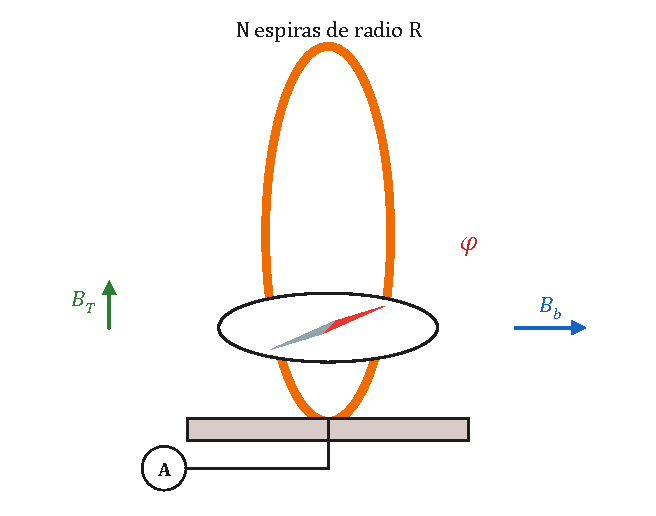
\includegraphics[width=\linewidth]{images/UD6/practica_bobina}
    \captionof{figure}{Brújula de tangentes.}
    \label{fig:mag-practica}
\end{minipage}

\textbf{Fundamento y cálculos.} La aguja se orienta según la suma del campo terrestre \(B_T\) (norte-sur) y el de la bobina,
\(B_b = N\mu_0 I/2R\), perpendicular a él. Por tanto \(\tg\varphi = B_b/B_T\). Representa \(\tg\varphi\) frente a \(I\): sale una
recta de pendiente \(N\mu_0/(2R B_T)\), de la que se obtiene \(B_T\).

\textbf{Cuestiones.}
\begin{enumerate}[label=\letraminuscula]
    \item Compara tu resultado con el valor de la componente horizontal en España (unos \qty{2.5e-5}{\tesla}).
    \item ¿Por qué hay que alejar la experiencia de objetos de hierro y de otros cables con corriente?
    \item ¿Qué ocurre si inviertes el sentido de la corriente?
\end{enumerate}


    \newpage

    %! Unidad 6 — Campo magnético e inducción electromagnética: ejercicios finales (adaptados de la fuente, con datos cambiados y resueltos)

\section{Ejercicios}\label{sec:mag-ejercicios}

Salvo que se indique otra cosa, usa \(e = \qty{1.6e-19}{\coulomb}\), \(m_e = \qty{9.11e-31}{\kg}\), \(m_p = \qty{1.67e-27}{\kg}\),
\(\mu_0 = 4\pi\cdot 10^{-7}\ \unit{\tesla\m\per\ampere}\) y \(g = \qty{9.8}{\m\per\second\squared}\).

\subsection{Cuestiones}

\begin{exercise}
    Una partícula cargada se mueve en un campo magnético uniforme sin experimentar ninguna fuerza. ¿Cómo es su velocidad respecto del campo?
    \begin{solu}
        \textcolor{red}{Paralela (o antiparalela) al campo}: \textcolor{blue}{entonces \(\sen\varphi = 0\) y \(F = qvB\sen\varphi = 0\).}
    \end{solu}
\end{exercise}

\begin{exercise}
    ¿Verdadero o falso?: «La fuerza magnética que actúa sobre una carga en movimiento no hace trabajo».
    \begin{solu}
        \textcolor{red}{Verdadero.} \textcolor{blue}{La fuerza es siempre perpendicular a la velocidad (y al desplazamiento): solo cambia la dirección
        de la velocidad, no su módulo ni la energía cinética.}
    \end{solu}
\end{exercise}

\begin{exercise}
    ¿Puede ser nula la fuerza magnética sobre una partícula cargada que se mueve en un campo magnético no nulo? ¿Y la fuerza eléctrica
    sobre una partícula cargada en un campo eléctrico no nulo?
    \begin{solu}
        \textcolor{red}{La magnética sí}, \textcolor{blue}{si se mueve paralela al campo.} \textcolor{red}{La eléctrica no}: \(\vec F = q\vec E\)
        \textcolor{blue}{no depende de la velocidad y solo es nula si \(q = 0\).}
    \end{solu}
\end{exercise}

\begin{exercise}
    Un neutrón entra perpendicularmente en un campo magnético uniforme a gran velocidad. ¿Qué trayectoria sigue?
    \begin{solu}
        \textcolor{red}{Una línea recta, con velocidad constante}: \textcolor{blue}{no tiene carga y el campo no ejerce fuerza sobre él.}
    \end{solu}
\end{exercise}

\begin{exercise}
    Una carga entra de izquierda a derecha en un campo uniforme perpendicular al papel y entrante, y se desvía en el sentido de las
    agujas del reloj. ¿Qué signo tiene?
    \begin{solu}
        \textcolor{blue}{Moviéndose hacia la derecha, girar en sentido horario es curvarse hacia abajo. Para una carga positiva,
        \(\vec v\times\vec B = \vec{i}\times(-\vec{k}) = \vec{j}\): hacia arriba.} \textcolor{red}{La carga es negativa.}
    \end{solu}
\end{exercise}

\begin{exercise}
    Una espira circular está en un campo uniforme. ¿Con qué orientación es máximo el flujo que la atraviesa? ¿Con cuál es nulo?
    \begin{solu}
        \textcolor{red}{Máximo con la espira perpendicular al campo} (\(\vec S\) paralelo a \(\vec B\)); \textcolor{red}{nulo con la espira paralela al campo}
        (\(\vec S\perp\vec B\)).
    \end{solu}
\end{exercise}

\begin{exercise}
    Indica el sentido de la corriente inducida en una espira cuando se aleja de ella el polo sur de un imán, y cuando se le acerca el polo norte.
    \begin{solu}
        \textcolor{blue}{Al alejar el polo sur, la espira se opone atrayéndolo: la cara que mira al imán se convierte en un polo norte. Al acercar el
        polo norte, se opone repeliéndolo: también forma un polo norte.} \textcolor{red}{En los dos casos la corriente, vista desde el imán, circula en
        sentido antihorario.}
    \end{solu}
\end{exercise}

\subsection{Fuerzas sobre cargas y corrientes}

\begin{exercise}
    Un protón se mueve a \qty{2e7}{\m\per\second} en un campo de \qty{1.5}{\tesla} y sufre una fuerza de \qty{3e-12}{\newton}. ¿Qué ángulo
    forma su velocidad con el campo?
    \begin{solu}
        \(\sen\varphi = \dfrac{F}{qvB} = \dfrac{3\cdot 10^{-12}}{1{,}6\cdot 10^{-19}\cdot 2\cdot 10^7\cdot 1{,}5} = 0{,}625 \Rightarrow \textcolor{red}{\varphi = \ang{38.7}}\).
    \end{solu}
\end{exercise}

\begin{exercise}
    Un electrón entra con \qty{4e6}{\m\per\second} perpendicularmente en un campo de \qty{5e-3}{\tesla}. Calcula la fuerza, el radio de su
    trayectoria y su período.
    \begin{solu}
        \(F = evB = \textcolor{red}{\qty{3.2e-15}{\newton}}\); \(R = \dfrac{m v}{e B} = \textcolor{red}{\qty{4.55e-3}{\m}}\);
        \(T = \dfrac{2\pi m}{e B} = \textcolor{red}{\qty{7.16e-9}{\second}}\).
    \end{solu}
\end{exercise}

\begin{exercise}
    En una región hay un campo \(\vec E = 3\,\vec{i} + 5\,\vec{j}\ \unit{\newton\per\coulomb}\) y un campo \(\vec B = 0{,}5\,\vec{k}\ \unit{\tesla}\).
    Un electrón entra con \(\vec v = 1000\,\vec{i}\ \unit{\m\per\second}\). Calcula la fuerza y la aceleración.
    \begin{solu}
        \(\vec v\times\vec B = 1000\,\vec{i}\times 0{,}5\,\vec{k} = -500\,\vec{j}\); \(\vec E + \vec v\times\vec B = 3\,\vec{i} - 495\,\vec{j}\).
        \[ \vec F = -e\,(3\,\vec{i} - 495\,\vec{j}) = \textcolor{red}{(-4{,}8\cdot 10^{-19}\,\vec{i} + 7{,}92\cdot 10^{-17}\,\vec{j})\ \unit{\newton}} \]
        \(a = \dfrac{F}{m} = \textcolor{red}{\qty{8.69e13}{\m\per\second\squared}}\).
    \end{solu}
\end{exercise}

\begin{exercise}
    Un electrón se acelera desde el reposo con una diferencia de potencial de \qty{200}{\volt} y entra perpendicularmente en un campo de
    \qty{0.01}{\tesla}. Calcula su velocidad, el radio de la trayectoria y el período.
    \begin{solu}
        \(v = \sqrt{\dfrac{2eV}{m}} = \textcolor{red}{\qty{8.38e6}{\m\per\second}}\); \(R = \dfrac{mv}{eB} = \textcolor{red}{\qty{4.77}{\mm}}\);
        \(T = \dfrac{2\pi m}{eB} = \textcolor{red}{\qty{3.58e-9}{\second}}\).
    \end{solu}
\end{exercise}

\begin{exercise}
    En una región hay un campo magnético \(\vec B = 0{,}4\,\vec{k}\ \unit{\tesla}\) y uno eléctrico \(\vec E = 200\,\vec{j}\ \unit{\newton\per\coulomb}\).
    ¿Con qué velocidad debe entrar una partícula cargada para seguir una línea recta?
    \begin{solu}
        \textcolor{blue}{Las fuerzas deben anularse: \(\vec E + \vec v\times\vec B = 0\). Con \(\vec v = v\,\vec{i}\): \(v\,\vec{i}\times 0{,}4\,\vec{k} = -0{,}4v\,\vec{j}\), luego \(200 = 0{,}4v\).}
        \(\textcolor{red}{\vec v = 500\,\vec{i}\ \unit{\m\per\second}}\) \textcolor{blue}{(sea cual sea su carga: es un \emph{selector de velocidades}).}
    \end{solu}
\end{exercise}

\begin{exercise}
    Un electrón entra de izquierda a derecha con \qty{2e6}{\m\per\second} en un campo de \qty{2e-3}{\tesla} perpendicular al papel y entrante.
    \begin{enumerate}[label=\letraminuscula]
        \item Calcula la fuerza que actúa sobre él.
        \item Calcula el radio de su trayectoria. ¿Cómo sería la de un protón?
        \item ¿Qué campo eléctrico habría que añadir para que siguiera en línea recta?
    \end{enumerate}
    \begin{solu}
        \begin{enumerate}[label=\letraminuscula]
            \item \(\vec v\times\vec B = 2\cdot 10^6\,\vec{i}\times(-2\cdot 10^{-3}\,\vec{k}) = 4000\,\vec{j}\);
            \(\textcolor{red}{\vec F = -e\cdot 4000\,\vec{j} = -6{,}4\cdot 10^{-16}\,\vec{j}\ \unit{\newton}}\) \textcolor{blue}{(hacia abajo).}
            \item \(R = \dfrac{mv}{eB} = \textcolor{red}{\qty{5.69}{\mm}}\). \textcolor{blue}{El protón se curvaría hacia arriba (sentido antihorario) con un radio
            \(m_p/m_e \approx 1835\) veces mayor:} \textcolor{red}{\qty{10.4}{\m}}.
            \item \(\vec E = -\vec v\times\vec B = \textcolor{red}{-4000\,\vec{j}\ \unit{\newton\per\coulomb}}\).
        \end{enumerate}
    \end{solu}
\end{exercise}

\begin{exercise}
    Una bobina rectangular de 40 espiras de \qty{4}{\cm} \(\times\) \qty{6}{\cm} lleva una corriente de \qty{30}{\milli\ampere}. Calcula su
    momento magnético y el momento del par si se coloca paralela a un campo de \qty{0.3}{\tesla}.
    \begin{solu}
        \(m = NIS = 40\cdot 0{,}03\cdot 2{,}4\cdot 10^{-3} = \textcolor{red}{\qty{2.88e-3}{\ampere\m\squared}}\);
        \textcolor{blue}{paralela al campo, \(\vec S\perp\vec B\):} \(M = mB = \textcolor{red}{\qty{8.64e-4}{\newton\m}}\).
    \end{solu}
\end{exercise}

\begin{exercise}
    Un conductor de \qty{15}{\cm} lleva \qty{5}{\ampere} y forma \ang{35} con un campo horizontal. ¿Qué campo hace falta para que la fuerza
    sobre él sea de \qty{0.3}{\newton}?
    \begin{solu}
        \(B = \dfrac{F}{IL\sen\alpha} = \dfrac{0{,}3}{5\cdot 0{,}15\cdot\sen\ang{35}} = \textcolor{red}{\qty{0.697}{\tesla}}\).
    \end{solu}
\end{exercise}

\begin{exercise}
    Una varilla horizontal de \qty{25}{\cm} y \qty{15}{\g} puede deslizar sin rozamiento por dos raíles verticales, y por ella circula una
    corriente de \qty{2}{\ampere} hacia la derecha. ¿Qué campo magnético perpendicular al plano de los raíles la mantiene en reposo?
    \begin{solu}
        \textcolor{blue}{La fuerza magnética debe ser vertical hacia arriba e igual al peso: \(ILB = mg\).}
        \(B = \dfrac{0{,}015\cdot 9{,}8}{2\cdot 0{,}25} = \textcolor{red}{\qty{0.294}{\tesla}}\).
        \textcolor{blue}{Como \(\vec{i}\times(-\vec{k}) = \vec{j}\),} \textcolor{red}{el campo debe ser entrante} \textcolor{blue}{(con el eje \(Y\) hacia arriba y el \(Z\) hacia el lector).}
    \end{solu}
\end{exercise}

\subsection{Campos creados por corrientes}

\begin{exercise}
    Un solenoide de \qty{25}{\cm} tiene 500 espiras y lleva una corriente de \qty{2}{\ampere}. ¿Cuánto vale el campo en su interior? Una
    partícula cargada entra en el solenoide moviéndose a lo largo de su eje: ¿qué trayectoria sigue?
    \begin{solu}
        \(B = \mu_0\,\dfrac{N}{L}\,I = 4\pi\cdot 10^{-7}\,\dfrac{500}{0{,}25}\cdot 2 = \textcolor{red}{\qty{5.03e-3}{\tesla}}\).
        \textcolor{red}{Una recta}: \textcolor{blue}{se mueve paralela al campo y no sufre fuerza.}
    \end{solu}
\end{exercise}

\begin{exercise}
    Dos conductores paralelos y muy largos están separados \qty{10}{\cm} y llevan \qty{10}{\ampere} y \qty{5}{\ampere} en el mismo sentido.
    Calcula el campo en un punto de la recta perpendicular a ellos situado \qty{5}{\cm} a la izquierda del primero, y en el punto medio.
    \begin{solu}
        \textcolor{blue}{A la izquierda de los dos, los campos tienen el mismo sentido:}
        \(B = \dfrac{\mu_0}{2\pi}\left(\dfrac{10}{0{,}05} + \dfrac{5}{0{,}15}\right) = \textcolor{red}{\qty{4.67e-5}{\tesla}}\).

        \textcolor{blue}{En el punto medio tienen sentidos opuestos:} \(B = \dfrac{\mu_0}{2\pi}\,\dfrac{10 - 5}{0{,}05} = \textcolor{red}{\qty{2e-5}{\tesla}}\).
    \end{solu}
\end{exercise}

\begin{exercise}
    Dos conductores rectilíneos y paralelos, perpendiculares al papel, están separados \qty{1}{\m}. Por el primero circulan \qty{4}{\ampere}
    saliendo del papel.
    \begin{enumerate}[label=\letraminuscula]
        \item ¿Qué corriente debe circular por el segundo, y en qué sentido, para que el campo se anule en un punto entre ellos situado a
        \qty{80}{\cm} del primero?
        \item Calcula la fuerza por unidad de longitud entre los dos hilos.
    \end{enumerate}
    \begin{solu}
        \begin{enumerate}[label=\letraminuscula]
            \item \textcolor{blue}{Entre los hilos los campos son opuestos si las corrientes tienen el mismo sentido:}
            \(\dfrac{4}{0{,}8} = \dfrac{I_2}{0{,}2} \Rightarrow \textcolor{red}{I_2 = \qty{1}{\ampere}}\), \textcolor{red}{también saliente}.
            \item \(\dfrac{F}{L} = \dfrac{\mu_0 I_1 I_2}{2\pi d} = \textcolor{red}{\qty{8e-7}{\newton\per\m}}\), \textcolor{red}{de atracción}.
        \end{enumerate}
    \end{solu}
\end{exercise}

\begin{exercise}
    Dos conductores rectilíneos y paralelos, separados \qty{15}{\cm}, llevan \qty{8}{\ampere} y \qty{5}{\ampere}. Calcula la fuerza por unidad de
    longitud sobre cada uno si las corrientes tienen el mismo sentido y si tienen sentidos contrarios.
    \begin{solu}
        \(\dfrac{F}{L} = \dfrac{\mu_0 I_1 I_2}{2\pi d} = 2\cdot 10^{-7}\,\dfrac{8\cdot 5}{0{,}15} = \textcolor{red}{\qty{5.33e-5}{\newton\per\m}}\) \textcolor{blue}{sobre cada uno:}
        \textcolor{red}{de atracción si tienen el mismo sentido y de repulsión si son contrarias.}
    \end{solu}
\end{exercise}

\begin{exercise}
    Por un conductor horizontal fijo circulan \qty{80}{\ampere}. Otro conductor paralelo de \qty{1}{\m} y \qty{15}{\g}, situado encima, puede
    moverse verticalmente. ¿Qué corriente, y en qué sentido, debe llevar para quedar en equilibrio a \qty{4}{\mm} del primero?
    \begin{solu}
        \textcolor{blue}{La fuerza debe ser de repulsión (hacia arriba), así que} \textcolor{red}{la corriente debe tener sentido contrario}.
        \[ \dfrac{\mu_0 I_1 I_2 L}{2\pi d} = mg \;\Rightarrow\; I_1 = \dfrac{mg\,2\pi d}{\mu_0 I_2 L} = \dfrac{0{,}015\cdot 9{,}8\cdot 2\pi\cdot 0{,}004}{4\pi\cdot 10^{-7}\cdot 80} = \textcolor{red}{\qty{36.8}{\ampere}} \]
    \end{solu}
\end{exercise}

\subsection{Flujo e inducción}

\begin{exercise}
    Calcula el flujo a través de una espira de vector superficie \(\vec S = (4\,\vec{i} + 3\,\vec{j} - 12\,\vec{k})\ \unit{\cm\squared}\) en un campo
    \(\vec B = 0{,}2\,\vec{i}\ \unit{\tesla}\).
    \begin{solu}
        \(\Phi = \vec B\cdot\vec S = 0{,}2\cdot 4\cdot 10^{-4} = \textcolor{red}{\qty{8e-5}{\weber}}\).
    \end{solu}
\end{exercise}

\begin{exercise}
    Una espira de \qty{20}{\cm\squared} está en el plano \(XY\). Calcula el flujo que la atraviesa si \(\vec B = 0{,}3\,\vec{i} + 0{,}05\,\vec{k}\ \unit{\tesla}\).
    \begin{solu}
        \textcolor{blue}{\(\vec S = 2\cdot 10^{-3}\,\vec{k}\ \unit{\m\squared}\); solo cuenta la componente \(z\) del campo:}
        \(\Phi = 0{,}05\cdot 2\cdot 10^{-3} = \textcolor{red}{\qty{1e-4}{\weber}}\).
    \end{solu}
\end{exercise}

\begin{exercise}
    Una bobina de 200 espiras cuadradas de \qty{5}{\cm} de lado está perpendicular a un campo de \qty{0.4}{\tesla}. ¿Qué fem media se induce
    si gira \ang{90} en \qty{0.02}{\second}?
    \begin{solu}
        \textcolor{blue}{El flujo pasa de \(BS\) a 0:} \(|\varepsilon| = N\,\dfrac{BS}{\Delta t} = 200\,\dfrac{0{,}4\cdot 0{,}0025}{0{,}02} = \textcolor{red}{\qty{10}{\volt}}\).
    \end{solu}
\end{exercise}

\begin{exercise}
    Una bobina de 300 espiras de \qty{8}{\cm} de radio está perpendicular a un campo de \qty{0.6}{\tesla}. Calcula la fem media inducida si el
    campo se anula en \qty{0.15}{\second}.
    \begin{solu}
        \(|\varepsilon| = N\,\dfrac{B\pi r^2}{\Delta t} = 300\,\dfrac{0{,}6\cdot\pi\cdot 0{,}08^2}{0{,}15} = \textcolor{red}{\qty{24.1}{\volt}}\).
    \end{solu}
\end{exercise}

\begin{exercise}
    El flujo a través de cada espira de una bobina de 400 espiras pasa de \qty{3e-4}{\weber} a \qty{1e-4}{\weber} en \qty{0.05}{\second}. ¿Qué fem media se induce?
    \begin{solu}
        \(\varepsilon = -N\,\dfrac{\Delta\Phi}{\Delta t} = -400\,\dfrac{(1 - 3)\cdot 10^{-4}}{0{,}05} = \textcolor{red}{\qty{1.6}{\volt}}\).
    \end{solu}
\end{exercise}

\begin{exercise}
    Una espira cuadrada de \qty{4}{\cm} de lado entra a \qty{5}{\cm\per\second} en una región con un campo perpendicular de \qty{0.5}{\tesla}.
    ¿Qué fem se induce mientras entra? ¿Y cuando está entera dentro del campo?
    \begin{solu}
        \textcolor{blue}{Mientras entra, el área dentro del campo crece a razón de \(lv\):} \(\varepsilon = B l v = 0{,}5\cdot 0{,}04\cdot 0{,}05 = \textcolor{red}{\qty{1e-3}{\volt}}\).
        \textcolor{red}{Cuando está dentro, el flujo no cambia y \(\varepsilon = 0\).}
    \end{solu}
\end{exercise}

\begin{exercise}
    Una bobina de 20 espiras de \qty{5}{\cm} de radio está perpendicular a un campo que varía según \(B = 0{,}05t - 0{,}02t^2\) (SI). Calcula el
    flujo que atraviesa la bobina en función del tiempo y la fem inducida en \(t = \qty{3}{\second}\).
    \begin{solu}
        \(\Phi = N B S = 20\cdot\pi\cdot 0{,}05^2\,(0{,}05t - 0{,}02t^2) = \textcolor{red}{0{,}157\,(0{,}05t - 0{,}02t^2)\ \unit{\weber}}\).

        \(\varepsilon = -\dfrac{d\Phi}{dt} = -0{,}157\,(0{,}05 - 0{,}04t)\); en \(t = 3\): \(\varepsilon = \textcolor{red}{\qty{0.011}{\volt}}\).
    \end{solu}
\end{exercise}

\begin{exercise}
    El flujo a través de una espira de \qty{20}{\cm\squared} varía según \(\Phi = 4\cdot 10^{-4}\cos(100t)\) (SI). Calcula el campo, supuesto
    uniforme, y la fem inducida.
    \begin{solu}
        \(B = \dfrac{\Phi_{\text{máx}}}{S} = \dfrac{4\cdot 10^{-4}}{2\cdot 10^{-3}} = \textcolor{red}{\qty{0.2}{\tesla}}\);
        \(\varepsilon = -\dfrac{d\Phi}{dt} = \textcolor{red}{0{,}04\sen(100t)\ \unit{\volt}}\).
    \end{solu}
\end{exercise}

\begin{exercise}
    Una espira cuadrada de \qty{10}{\cm} de lado está en el plano \(XY\), en un campo que forma \ang{30} con el eje \(Z\) y cuyo módulo varía
    según \(B = 0{,}02\,(t^2 + 3t + 1)\) (SI). Calcula el flujo en función del tiempo y la fem en \(t = \qty{5}{\second}\). ¿En qué sentido circula
    la corriente?
    \begin{solu}
        \(\Phi = B S\cos\ang{30} = \textcolor{red}{1{,}73\cdot 10^{-4}\,(t^2 + 3t + 1)\ \unit{\weber}}\);
        \(\varepsilon = -\dfrac{d\Phi}{dt} = -1{,}73\cdot 10^{-4}(2t + 3)\); en \(t = 5\): \(|\varepsilon| = \textcolor{red}{\qty{2.25e-3}{\volt}}\).

        \textcolor{blue}{El flujo en el sentido \(+Z\) aumenta, así que el campo inducido apunta hacia \(-Z\):} \textcolor{red}{la corriente circula en sentido
        horario visto desde arriba (desde \(+Z\)).}
    \end{solu}
\end{exercise}

\subsection{Alternador y transformador}

\begin{exercise}
    Una bobina de 100 espiras cuadradas de \qty{4}{\cm} de lado gira en un campo de \qty{0.5}{\tesla}. ¿Con qué frecuencia debe girar para
    que la fem máxima sea de \qty{10}{\volt}?
    \begin{solu}
        \(\omega = \dfrac{\varepsilon_0}{NBS} = \dfrac{10}{100\cdot 0{,}5\cdot 0{,}0016} = \qty{125}{\radian\per\second}\);
        \(f = \dfrac{\omega}{2\pi} = \textcolor{red}{\qty{19.9}{\hertz}}\).
    \end{solu}
\end{exercise}

\begin{exercise}
    Un generador tiene una bobina de 20 espiras de \qty{0.05}{\m\squared} que gira a \qty{50}{\hertz} en un campo de \qty{0.4}{\tesla}. Calcula la
    fem máxima.
    \begin{solu}
        \(\varepsilon_0 = NBS\omega = 20\cdot 0{,}4\cdot 0{,}05\cdot 100\pi = \textcolor{red}{\qty{126}{\volt}}\).
    \end{solu}
\end{exercise}

\begin{exercise}
    Una bobina de 50 espiras de \qty{200}{\cm\squared} gira a \qty{600}{rpm} alrededor de un eje de su plano perpendicular a un campo de
    \qty{0.3}{\tesla}. Escribe la fem inducida en función del tiempo.
    \begin{solu}
        \(\omega = 600\cdot\dfrac{2\pi}{60} = 20\pi\ \unit{\radian\per\second}\); \(\varepsilon_0 = NBS\omega = 50\cdot 0{,}3\cdot 0{,}02\cdot 20\pi = \qty{18.8}{\volt}\).
        \[ \textcolor{red}{\varepsilon = 18{,}8\sen(20\pi t)\ \text{(V)}} \]
    \end{solu}
\end{exercise}

\begin{exercise}
    Se quiere obtener \qty{12}{\volt} a partir de la red de \qty{220}{\volt} con un transformador cuyo primario tiene 1000 espiras. ¿Cuántas
    espiras debe tener el secundario? Si por el secundario circulan \qty{2}{\ampere}, ¿qué intensidad circula por el primario?
    \begin{solu}
        \(N_2 = N_1\,\dfrac{V_2}{V_1} = 1000\,\dfrac{12}{220} \approx \textcolor{red}{55\ \text{espiras}}\);
        \(I_1 = I_2\,\dfrac{V_2}{V_1} = \textcolor{red}{\qty{0.109}{\ampere}}\).
    \end{solu}
\end{exercise}


%----------------------------------------------------------------------------------------
%	PARTE: FÍSICA MODERNA
%----------------------------------------------------------------------------------------

    \part{Física moderna}

    \chapterimage{images/portada_cabeceras/cabecera_UD7}
    \chapter{Física cuántica}

    %! Unidad 7 — Física cuántica (teoría, actividades resueltas y prácticas)
%! Fuente: Fuentes/Tema_7.pdf (reescrito; datos de las actividades cambiados y recalculados)

\section*{Para empezar: dos nubecillas en el horizonte}
\addcontentsline{toc}{section}{Para empezar: dos nubecillas en el horizonte}

En 1900, Lord Kelvin dijo en una conferencia que la física estaba prácticamente terminada: la mecánica de Newton y el
electromagnetismo de Maxwell lo explicaban casi todo. Solo quedaban «dos nubecillas en el horizonte»: el resultado negativo de un
experimento que buscaba el éter y la forma en que brillan los cuerpos calientes. Aquellas dos nubecillas dieron lugar a las dos
grandes teorías del siglo \textsc{xx}: la \textbf{relatividad} y la \textbf{física cuántica}. Gracias a la segunda entendemos cómo
funcionan los átomos, los láseres, los LED, las placas solares o los chips de un teléfono móvil. En esta unidad veremos los
experimentos que obligaron a abandonar la física clásica y las ideas, a veces sorprendentes, que la sustituyeron.

\section{Las ondas electromagnéticas}\label{sec:cua-espectro}

Una carga eléctrica acelerada emite energía en forma de \rojon{onda electromagnética}: un campo eléctrico y un campo magnético
que oscilan perpendiculares entre sí y a la dirección de propagación (figura~\ref{fig:cua-onda}). Son ondas transversales que no
necesitan medio material y que, en el vacío, viajan a \(c = \qty{3e8}{\m\per\second}\). Como toda onda, cumplen \(c = \lambda\nu\).

\begin{figure}[H]
    \centering
    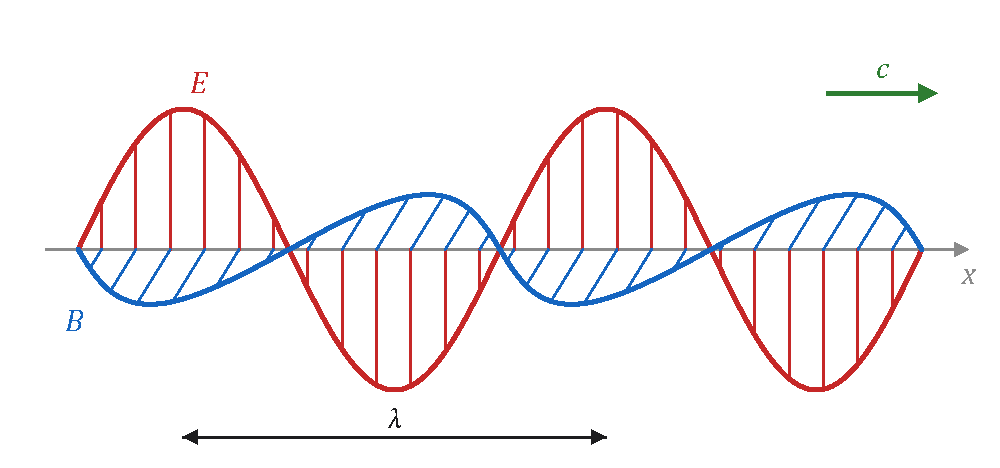
\includegraphics[width=0.66\linewidth]{images/UD7/onda_em}
    \caption{En una onda electromagnética \(\vec E\) y \(\vec B\) oscilan en fase, perpendiculares entre sí y a la propagación.}
    \label{fig:cua-onda}
\end{figure}

El \rojon{espectro electromagnético} es el conjunto de todas las ondas electromagnéticas, ordenadas según su frecuencia
(figura~\ref{fig:cua-espectro}):
\begin{itemize}
    \item \textbf{Ondas de radio} (hasta \qty{e9}{\hertz}): radio, televisión. Se producen con corrientes oscilantes en antenas.
    \item \textbf{Microondas} (\qtyrange{e9}{e11}{\hertz}): radar, telefonía móvil, wifi, hornos de microondas.
    \item \textbf{Infrarrojo} (\qtyrange{e11}{4e14}{\hertz}): lo emiten los cuerpos calientes; mandos a distancia, cámaras térmicas.
    \item \textbf{Luz visible} (\qtyrange{4e14}{7.5e14}{\hertz}, de \qty{750}{\nm} a \qty{400}{\nm}): del rojo al violeta.
    \item \textbf{Ultravioleta} (\qtyrange{7.5e14}{e17}{\hertz}): broncea la piel y puede dañarla; esteriliza.
    \item \textbf{Rayos X} (\qtyrange{e17}{e19}{\hertz}): radiografías.
    \item \textbf{Rayos gamma} (más de \qty{e19}{\hertz}): los emiten los núcleos radiactivos; radioterapia.
\end{itemize}

\begin{figure}[H]
    \centering
    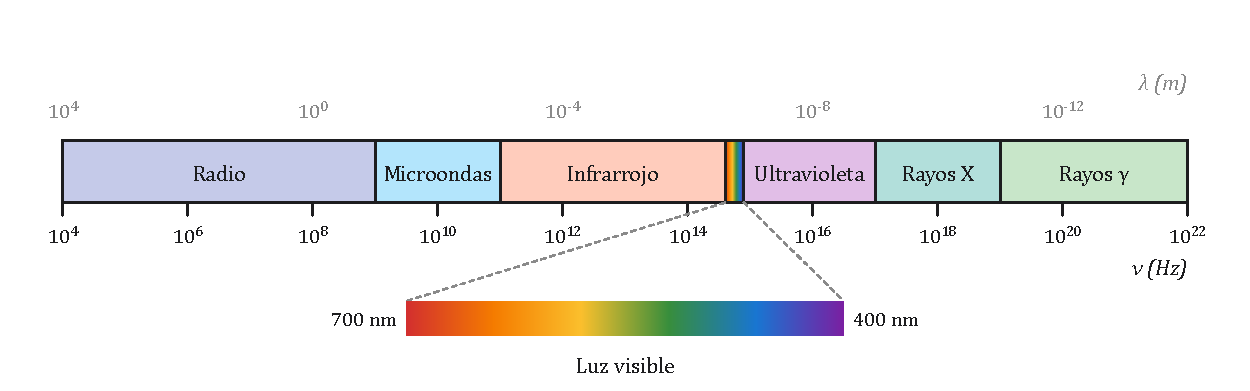
\includegraphics[width=0.95\linewidth]{images/UD7/espectro}
    \caption{El espectro electromagnético. La luz visible es una franja estrechísima.}
    \label{fig:cua-espectro}
\end{figure}

\section{La radiación del cuerpo negro}\label{sec:cua-cuerpo-negro}

Todos los cuerpos emiten radiación electromagnética por estar a una temperatura: es la \azuln{radiación térmica}. A temperatura
ambiente es casi toda infrarroja e invisible; al calentar un trozo de hierro, empieza a brillar rojo, luego amarillento y, a muy
alta temperatura, casi blanco.

Para estudiarla se usa un modelo ideal, el \rojon{cuerpo negro}: un cuerpo que absorbe toda la radiación que le llega y que, por
tanto, emite radiación de todas las longitudes de onda, con un espectro que solo depende de su temperatura. Una buena aproximación
es una cavidad con un pequeño orificio: la radiación que entra queda atrapada tras varias reflexiones (figura~\ref{fig:cua-cavidad}).

\begin{figure}[H]
    \centering
    \begin{minipage}[b]{0.34\linewidth}
        \centering
        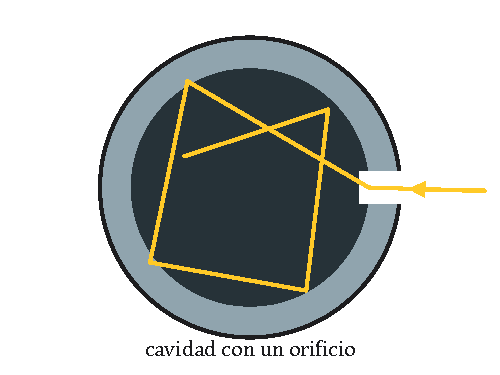
\includegraphics[width=\linewidth]{images/UD7/cuerpo_negro}
        \caption{Cavidad que actúa como cuerpo negro.}
        \label{fig:cua-cavidad}
    \end{minipage}\hfill
    \begin{minipage}[b]{0.62\linewidth}
        \centering
        \begin{tikzpicture}
            \begin{axis}[fisica, width=\linewidth, height=5.2cm, xmin=0, xmax=3.1, ymin=0, ymax=1.15,
                xlabel={\(\lambda\) (\unit{\micro\m})}, ylabel={\(I\)}, xtick={0.5,1,1.5,2,2.5,3}, ytick=\empty, samples=120,
                legend style={font=\scriptsize, draw=none, at={(0.98,0.95)}, anchor=north east}]
                \addplot[domain=0.12:3, very thick, red] {(1/(x^5*(exp(14.388/(x*5))-1)))/0.1075};
                \addlegendentry{\qty{5000}{\kelvin}}
                \addplot[domain=0.12:3, very thick, ocre] {(1/(x^5*(exp(14.388/(x*4))-1)))/0.1075};
                \addlegendentry{\qty{4000}{\kelvin}}
                \addplot[domain=0.12:3, very thick, blue] {(1/(x^5*(exp(14.388/(x*3))-1)))/0.1075};
                \addlegendentry{\qty{3000}{\kelvin}}
                \addplot[domain=1.32:3, thick, dashed, gray] {5/(14.388*x^4)/0.1075};
                \node[font=\scriptsize, gray, anchor=west] at (axis cs:1.4,1.08) {Rayleigh-Jeans (5000 K)};
            \end{axis}
        \end{tikzpicture}
        \caption{Espectro del cuerpo negro (ley de Planck). La predicción clásica (discontinua) se dispara a longitudes de onda cortas.}
        \label{fig:cua-planck}
    \end{minipage}
\end{figure}

Las medidas experimentales llevaron a dos leyes:
\begin{itemize}
    \item \textbf{Ley de Wien}. La longitud de onda a la que la emisión es máxima es inversamente proporcional a la temperatura
    absoluta:
    \begin{centeredequation}
        \boxed{\lambda_{\text{máx}}\,T = b} \qquad b = \qty{2.9e-3}{\m\kelvin} \label{eq:cua-wien}
    \end{centeredequation}
    Por eso las estrellas más calientes son azuladas y las más frías, rojizas.
    \item \textbf{Ley de Stefan-Boltzmann}. La potencia emitida por unidad de superficie es proporcional a la cuarta potencia de la
    temperatura absoluta:
    \begin{centeredequation}
        \boxed{I = \sigma\,T^4} \qquad \sigma = \qty{5.67e-8}{\watt\per\m\squared\per\kelvin\tothe{4}} \label{eq:cua-stefan}
    \end{centeredequation}
\end{itemize}

\paragraph{La catástrofe ultravioleta.} Rayleigh y Jeans intentaron explicar el espectro con la física clásica, suponiendo que los
átomos de las paredes oscilan y emiten energía de forma continua. Su fórmula, \(I \propto T/\lambda^4\), funcionaba bien a longitudes de
onda largas, pero predecía que la intensidad crecería sin límite al acercarse al ultravioleta: un cuerpo caliente emitiría una
energía infinita. Este fracaso se llamó \azuln{catástrofe ultravioleta} (figura~\ref{fig:cua-planck}).

\section{La hipótesis de Planck}\label{sec:cua-planck}

En 1900, Max Planck encontró una fórmula que se ajustaba perfectamente a las medidas. Para justificarla tuvo que hacer una suposición
revolucionaria, que él mismo consideró un «acto de desesperación»:

\begin{definition}[Hipótesis de Planck]
    La energía de los osciladores que emiten radiación no puede tomar cualquier valor: solo puede emitirse o absorberse en paquetes,
    los \rojon{cuantos}, cuya energía es proporcional a la frecuencia:
    \begin{centeredequation}
        \boxed{E = h\,\nu = \dfrac{h\,c}{\lambda}} \label{eq:cua-planck}
    \end{centeredequation}
    donde \(h = \qty{6.63e-34}{\joule\second}\) es la \azuln{constante de Planck}.
\end{definition}

La energía está \textbf{cuantizada}: un oscilador solo puede tener energías \(h\nu\), \(2h\nu\), \(3h\nu\)\ldots{} Como \(h\) es
tan pequeña, en el mundo cotidiano los saltos son imperceptibles y la energía parece continua. Es habitual expresar estas energías en
\azuln{electronvoltios}: \(\qty{1}{\electronvolt} = \qty{1.6e-19}{\joule}\), la energía que gana un electrón al acelerarse con una
diferencia de potencial de \qty{1}{\volt}.

\begin{exercise}
    Calcula, en julios y en electronvoltios, la energía de un fotón de una emisora de FM de \qty{95}{\mega\hertz}.
    \begin{solu}
        \(E = h\nu = 6{,}63\cdot 10^{-34}\cdot 95\cdot 10^6 = \textcolor{red}{\qty{6.30e-26}{\joule}}\) \(= \dfrac{6{,}30\cdot 10^{-26}}{1{,}6\cdot 10^{-19}} = \textcolor{red}{\qty{3.94e-7}{\electronvolt}}\).
    \end{solu}
\end{exercise}

\begin{exercise}
    El espectro visible va de \qty{400}{\nm} a \qty{750}{\nm}. ¿Entre qué energías, en eV, están sus fotones?
    \begin{solu}
        \(E = \dfrac{hc}{\lambda}\): \(E_{400} = \dfrac{6{,}63\cdot 10^{-34}\cdot 3\cdot 10^8}{400\cdot 10^{-9}\cdot 1{,}6\cdot 10^{-19}} = \textcolor{red}{\qty{3.11}{\electronvolt}}\);
        \(E_{750} = \textcolor{red}{\qty{1.66}{\electronvolt}}\).
    \end{solu}
\end{exercise}

\begin{exercise}
    El filamento de una bombilla está a \qty{2027}{\celsius}. ¿A qué longitud de onda emite con más intensidad? ¿Por qué estas bombillas
    calientan tanto?
    \begin{solu}
        \(\lambda_{\text{máx}} = \dfrac{b}{T} = \dfrac{2{,}9\cdot 10^{-3}}{2300} = \textcolor{red}{\qty{1261}{\nm}}\):
        \textcolor{red}{en el infrarrojo}. \textcolor{blue}{La mayor parte de la energía sale como calor y solo una pequeña parte como luz visible.}
    \end{solu}
\end{exercise}

\begin{exercise}
    Un cuerpo caliente emite con una potencia de \qty{0.05}{\watt} radiación cuyo máximo está en \qty{650}{\nm}. Suponiendo que toda
    fuera de esa longitud de onda, ¿cuántos fotones emite en un minuto?
    \begin{solu}
        \textcolor{blue}{Energía de cada fotón: \(E = hc/\lambda = \qty{3.06e-19}{\joule}\). Energía emitida en un minuto: \(0{,}05\cdot 60 = \qty{3}{\joule}\).}
        \(N = \dfrac{3}{3{,}06\cdot 10^{-19}} = \textcolor{red}{\num{9.8e18}\ \text{fotones}}\).
    \end{solu}
\end{exercise}

\begin{exercise}
    La superficie del Sol está a unos \qty{5800}{\kelvin}. ¿A qué longitud de onda emite con más intensidad? ¿Qué potencia emite por
    cada metro cuadrado?
    \begin{solu}
        \(\lambda_{\text{máx}} = \dfrac{2{,}9\cdot 10^{-3}}{5800} = \textcolor{red}{\qty{500}{\nm}}\) \textcolor{blue}{(en el centro del visible)};
        \(I = \sigma T^4 = 5{,}67\cdot 10^{-8}\cdot 5800^4 = \textcolor{red}{\qty{6.4e7}{\watt\per\m\squared}}\).
    \end{solu}
\end{exercise}

\section{El efecto fotoeléctrico}\label{sec:cua-fotoelectrico}

El \rojon{efecto fotoeléctrico} es la emisión de electrones por un metal cuando se ilumina con luz de frecuencia adecuada. Se
estudia con un tubo de vacío que contiene una placa metálica (el cátodo) y otra que recoge los electrones (el ánodo), conectadas a una
fuente de tensión regulable (figura~\ref{fig:cua-fotoelectrico}). Al iluminar el cátodo, el amperímetro marca corriente.

\begin{figure}[H]
    \centering
    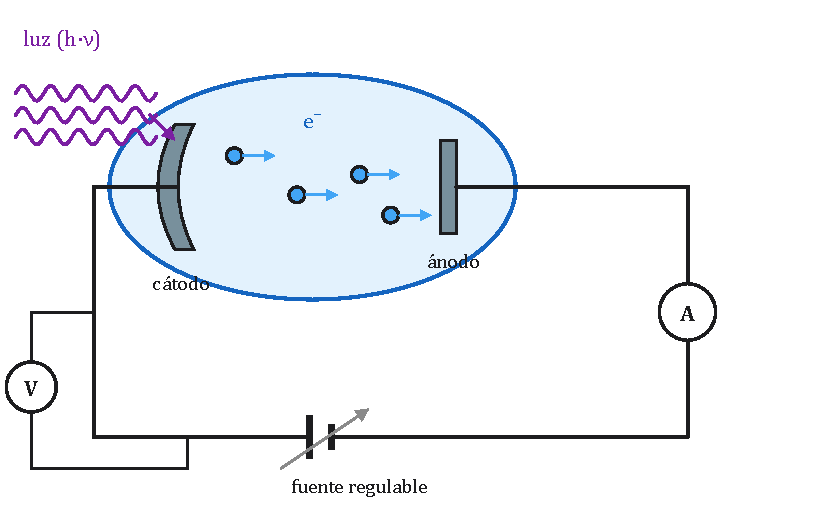
\includegraphics[width=0.55\linewidth]{images/UD7/fotoelectrico}
    \caption{Montaje para estudiar el efecto fotoeléctrico.}
    \label{fig:cua-fotoelectrico}
\end{figure}

Los resultados experimentales eran:
\begin{enumerate}[label=\numberballmDarkTeal]
    \item Para cada metal hay una \azuln{frecuencia umbral} \(\nu_0\): con luz de frecuencia menor no se emiten electrones, \emph{por
    intensa que sea}.
    \item Por encima del umbral, la emisión es instantánea, aunque la luz sea muy débil.
    \item La energía cinética máxima de los electrones depende de la frecuencia de la luz, no de su intensidad.
    \item El número de electrones emitidos (la intensidad de la corriente) es proporcional a la intensidad de la luz.
\end{enumerate}
Según la teoría ondulatoria clásica, la energía de la luz depende de su intensidad y llega de forma continua: con luz intensa siempre
debería haber emisión (tras un tiempo de acumulación), y los electrones deberían salir más rápido cuanto más intensa fuera la luz. Nada de
esto se cumplía.

\paragraph{Explicación de Einstein (1905).} Einstein extendió la idea de Planck: la luz no solo se emite en cuantos, sino que
\emph{está formada} por cuantos, los \rojon{fotones}, de energía \(h\nu\). Cada fotón cede toda su energía a un solo electrón. Parte de
ella se gasta en arrancarlo del metal (el \azuln{trabajo de extracción} \(W_0 = h\nu_0\)) y el resto se convierte en energía cinética:
\begin{centeredequation}
    \boxed{h\,\nu = h\,\nu_0 + E_{c,\text{máx}}} \qquad\qquad E_{c,\text{máx}} = \tfrac{1}{2}\,m\,v_{\text{máx}}^2 \label{eq:cua-einstein}
\end{centeredequation}
Así se explican todos los hechos: si \(h\nu < W_0\), ningún fotón tiene energía suficiente; más intensidad significa más fotones (y más
electrones), pero no fotones más energéticos. Einstein recibió por este trabajo el premio Nobel de 1921.

\paragraph{Potencial de frenado.} Si se hace el ánodo negativo respecto del cátodo, los electrones se frenan. La corriente se anula
para una tensión \(V_0\), el \azuln{potencial de frenado}, que detiene incluso a los electrones más rápidos:
\begin{centeredequation}
    \boxed{e\,V_0 = E_{c,\text{máx}} = h\,\nu - h\,\nu_0} \label{eq:cua-frenado}
\end{centeredequation}
El potencial de frenado no depende de la intensidad de la luz y crece linealmente con la frecuencia, con pendiente \(h/e\). Midiéndolo
para varias frecuencias, Millikan obtuvo en 1916 un valor muy preciso de \(h\).

\begin{figure}[H]
    \centering
    \begin{tikzpicture}
        \begin{axis}[fisica, width=0.46\linewidth, height=4.4cm, xmin=-1.6, xmax=3.2, ymin=0, ymax=1.35,
            xlabel={\(V\)}, ylabel={\(i\)}, xtick={-1.2}, xticklabels={\(-V_0\)}, ytick=\empty, samples=80]
            \addplot[domain=-1.2:3, very thick, ocre] {1.1*(1-exp(-2*(x+1.2)))};
            \addplot[domain=-1.2:3, very thick, blue] {0.6*(1-exp(-2*(x+1.2)))};
            \node[font=\scriptsize, ocre, anchor=south] at (axis cs:2.4,1.1) {\(I_2\)};
            \node[font=\scriptsize, blue, anchor=south] at (axis cs:2.4,0.6) {\(I_1 < I_2\)};
        \end{axis}
    \end{tikzpicture}\hfill
    \begin{tikzpicture}
        \begin{axis}[fisica, width=0.46\linewidth, height=4.4cm, xmin=0, xmax=3.2, ymin=0, ymax=2.2,
            xlabel={\(\nu\)}, ylabel={\(E_{c,\text{máx}}\)}, xtick={1}, xticklabels={\(\nu_0\)}, ytick=\empty]
            \addplot[domain=1:3, very thick, ocre] {x-1};
            \addplot[domain=0:1, thick, dashed, gray] {x-1};
            \node[font=\scriptsize, anchor=west] at (axis cs:1.8,0.5) {pendiente \(h\)};
        \end{axis}
    \end{tikzpicture}
    \caption{Izquierda: la corriente se anula en \(-V_0\) sea cual sea la intensidad de la luz. Derecha: la energía cinética máxima
    crece linealmente con la frecuencia a partir del umbral.}
    \label{fig:cua-curvas}
\end{figure}

\begin{exercise}
    Un electrón arrancado de un metal cuyo trabajo de extracción es \qty{4.5}{\electronvolt} sale con una energía cinética de
    \qty{3}{\electronvolt}. ¿Cuál era la frecuencia del fotón?
    \begin{solu}
        \(\nu = \dfrac{W_0 + E_c}{h} = \dfrac{7{,}5\cdot 1{,}6\cdot 10^{-19}}{6{,}63\cdot 10^{-34}} = \textcolor{red}{\qty{1.81e15}{\hertz}}\) \textcolor{blue}{(ultravioleta).}
    \end{solu}
\end{exercise}

\begin{exercise}
    La frecuencia umbral del sodio es \qty{5.5e14}{\hertz}. ¿Cuál es el potencial de frenado si se ilumina con luz de \qty{7.2e14}{\hertz}?
    \begin{solu}
        \(V_0 = \dfrac{h(\nu - \nu_0)}{e} = \dfrac{6{,}63\cdot 10^{-34}\cdot 1{,}7\cdot 10^{14}}{1{,}6\cdot 10^{-19}} = \textcolor{red}{\qty{0.70}{\volt}}\).
    \end{solu}
\end{exercise}

\begin{exercise}
    La longitud de onda máxima que produce efecto fotoeléctrico en un metal es \qty{680}{\nm}. Calcula el trabajo de extracción y la
    energía cinética máxima de los electrones si se ilumina con luz de \qty{450}{\nm}.
    \begin{solu}
        \(W_0 = \dfrac{hc}{\lambda_0} = \textcolor{red}{\qty{2.93e-19}{\joule} = \qty{1.83}{\electronvolt}}\);
        \(E_c = \dfrac{hc}{\lambda} - W_0 = \textcolor{red}{\qty{0.93}{\electronvolt}}\).
    \end{solu}
\end{exercise}

\begin{exercise}
    Un metal iluminado con luz de \qty{8e14}{\hertz} tiene un potencial de frenado de \qty{0.6}{\volt}. Con otra luz, el potencial es de
    \qty{1.6}{\volt}. ¿Qué frecuencia tiene la segunda luz?
    \begin{solu}
        \textcolor{blue}{Restando las dos ecuaciones \(eV_0 = h\nu - W_0\): \(e\,\Delta V_0 = h\,\Delta\nu\).}
        \(\nu_2 = 8\cdot 10^{14} + \dfrac{1{,}6\cdot 10^{-19}\cdot 1}{6{,}63\cdot 10^{-34}} = \textcolor{red}{\qty{1.04e15}{\hertz}}\).
    \end{solu}
\end{exercise}

\section{El efecto Compton}\label{sec:cua-compton}

En 1923, Arthur Compton hizo incidir rayos X sobre un bloque de grafito y observó que la radiación dispersada tenía una longitud de
onda mayor que la incidente, tanto más cuanto mayor era el ángulo de dispersión \(\theta\). Según la teoría clásica, la onda dispersada
debería tener la misma frecuencia.

Compton lo explicó tratando el fenómeno como un \textbf{choque entre dos partículas}: un fotón y un electrón casi libre
(figura~\ref{fig:cua-compton}). El fotón cede parte de su energía y de su cantidad de movimiento al electrón, así que sale con menos
energía y mayor longitud de onda. Aplicando la conservación de la energía y de la cantidad de movimiento (con relatividad) obtuvo:
\begin{centeredequation}
    \boxed{\lambda' - \lambda = \lambda_C\,(1 - \cos\theta)} \qquad \lambda_C = \dfrac{h}{m_e c} = \qty{2.43e-12}{\m} \label{eq:cua-compton}
\end{centeredequation}
donde \(\lambda_C\) es la \azuln{longitud de onda Compton} del electrón.

\begin{figure}[H]
    \centering
    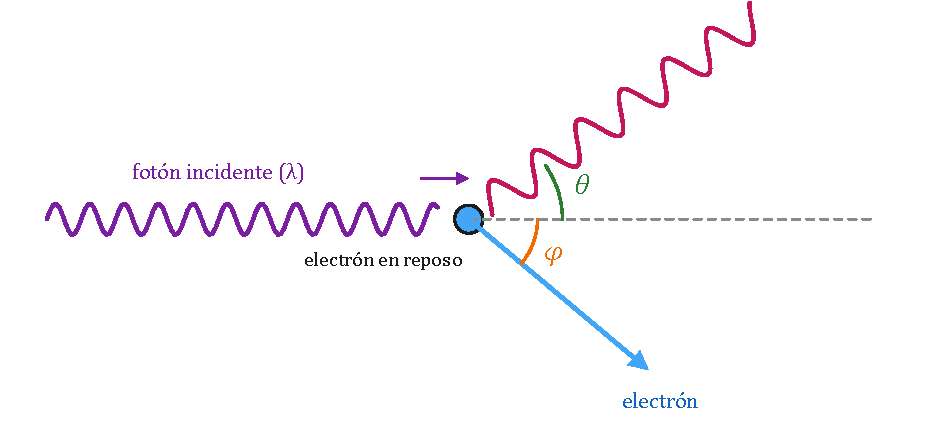
\includegraphics[width=0.62\linewidth]{images/UD7/compton}
    \caption{Efecto Compton: el fotón sale desviado un ángulo \(\theta\) y con mayor longitud de onda.}
    \label{fig:cua-compton}
\end{figure}

\begin{remark}
    El efecto Compton demuestra que el fotón se comporta como una partícula: tiene energía \(E = h\nu\) y también \textbf{cantidad de
    movimiento}, \(p = E/c = h/\lambda\), aunque no tenga masa. El cambio de longitud de onda es apreciable con rayos X (de \(\lambda\)
    muy pequeña), pero no con luz visible.
\end{remark}

\begin{exercise}
    Un fotón de \qty{20}{\kilo\electronvolt} choca con un electrón en reposo y sale desviado \ang{90}. Calcula su longitud de onda antes
    y después del choque y su nueva energía.
    \begin{solu}
        \(\lambda = \dfrac{hc}{E} = \dfrac{6{,}63\cdot 10^{-34}\cdot 3\cdot 10^8}{2\cdot 10^4\cdot 1{,}6\cdot 10^{-19}} = \textcolor{red}{\qty{6.22e-11}{\m}}\);
        \(\lambda' = \lambda + \lambda_C(1 - \cos\ang{90}) = \textcolor{red}{\qty{6.46e-11}{\m}}\).

        \(E' = \dfrac{hc}{\lambda'} = \textcolor{red}{\qty{19.3}{\kilo\electronvolt}}\) \textcolor{blue}{(el electrón se lleva \qty{0.7}{\kilo\electronvolt}).}
    \end{solu}
\end{exercise}

\section{Dualidad onda-corpúsculo. Hipótesis de De Broglie}\label{sec:cua-debroglie}

La luz se comporta como una onda en la propagación, las interferencias o la difracción, y como un chorro de partículas en el efecto
fotoeléctrico o el Compton: tiene un \textbf{comportamiento dual}. En 1924, Louis de Broglie propuso que esta dualidad no es exclusiva
de la luz, sino que vale para toda la materia:

\begin{definition}[Hipótesis de De Broglie]
    Toda partícula en movimiento lleva asociada una onda, cuya longitud de onda depende de su cantidad de movimiento:
    \begin{centeredequation}
        \boxed{\lambda = \dfrac{h}{p} = \dfrac{h}{m\,v}} \label{eq:cua-debroglie}
    \end{centeredequation}
\end{definition}

Si una partícula de carga \(q\) se acelera desde el reposo con una diferencia de potencial \(V\), su energía cinética es \(qV\) y
\(p = \sqrt{2mqV}\), así que \(\lambda = h/\sqrt{2mqV}\).

En 1927, Davisson y Germer observaron la \textbf{difracción de electrones} en un cristal de níquel, con la longitud de onda que predecía
De Broglie. Hoy los microscopios electrónicos aprovechan que la longitud de onda de los electrones es miles de veces menor que la de la
luz visible para ver detalles de tamaño atómico. Para objetos cotidianos, en cambio, \(\lambda\) es tan pequeña que los efectos
ondulatorios son imposibles de observar.

\begin{exercise}
    Calcula la longitud de onda de De Broglie de un electrón con una energía cinética de \qty{150}{\electronvolt} y de una pelota de tenis de
    \qty{60}{\g} que va a \qty{40}{\m\per\second}.
    \begin{solu}
        \textcolor{blue}{Electrón: \(v = \sqrt{2E_c/m} = \qty{7.26e6}{\m\per\second}\).} \(\lambda = \dfrac{h}{mv} = \textcolor{red}{\qty{1.0e-10}{\m}}\)
        \textcolor{blue}{(del tamaño de un átomo: se difracta en los cristales).}

        Pelota: \(\lambda = \dfrac{6{,}63\cdot 10^{-34}}{0{,}06\cdot 40} = \textcolor{red}{\qty{2.8e-34}{\m}}\) \textcolor{blue}{(totalmente inobservable).}
    \end{solu}
\end{exercise}

\subsection{La doble rendija}\label{subsec:cua-young}

En 1801, Thomas Young hizo pasar la luz de una rendija \(S_0\) por dos rendijas muy próximas, \(S_1\) y \(S_2\). Como proceden del mismo
frente de onda, son focos coherentes, y en la pantalla aparecen franjas brillantes y oscuras: la interferencia de la
unidad~2 (figura~\ref{fig:cua-young}). Fue la gran prueba de la naturaleza ondulatoria de la luz.

\begin{figure}[H]
    \centering
    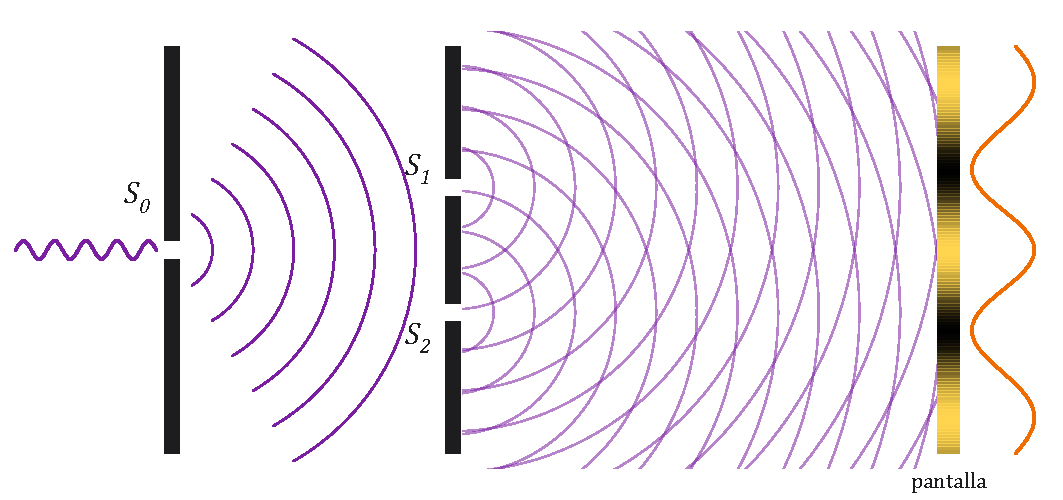
\includegraphics[width=0.75\linewidth]{images/UD7/young}
    \caption{Experimento de la doble rendija. La intensidad en la pantalla (a la derecha) se ha calculado con la diferencia de caminos.}
    \label{fig:cua-young}
\end{figure}

Lo sorprendente es que el experimento funciona igual con \emph{electrones} (y hasta con moléculas grandes). Si se envían de uno en uno,
cada electrón llega a un punto concreto de la pantalla, como una partícula; pero, al acumular miles, aparecen las franjas de
interferencia, como si cada electrón hubiera pasado por las dos rendijas a la vez. Y si se intenta averiguar por cuál pasa, las franjas
desaparecen. La mecánica cuántica no dice dónde llegará cada electrón, solo la \textbf{probabilidad} de que llegue a cada punto.

\section{El principio de incertidumbre}\label{sec:cua-heisenberg}

En física clásica, conociendo con precisión la posición y la velocidad de una partícula se puede predecir su movimiento futuro. En 1927,
Werner Heisenberg demostró que eso es imposible en el mundo cuántico:

\begin{definition}[Principio de incertidumbre de Heisenberg]
    No es posible conocer a la vez, con precisión ilimitada, la posición y la cantidad de movimiento de una partícula. El producto de sus
    incertidumbres cumple:
    \begin{centeredequation}
        \boxed{\Delta x\cdot\Delta p \geq \dfrac{h}{2\pi}} \label{eq:cua-heisenberg}
    \end{centeredequation}
    Una relación análoga liga la energía y el tiempo: \(\Delta E\cdot\Delta t \geq h/2\pi\).
\end{definition}

No es un problema de los aparatos de medida: es una propiedad de la naturaleza. Para observar un electrón hay que iluminarlo, y el fotón
que rebota le cambia la velocidad; cuanto menor sea su longitud de onda (para precisar la posición), mayor será el golpe. La mecánica
cuántica, desarrollada por Heisenberg, Schrödinger y Dirac, describe las partículas con funciones de onda que dan
\textbf{probabilidades}, no trayectorias. Einstein nunca aceptó del todo este carácter probabilista: «Dios no juega a los dados».

\begin{exercise}
    Se conoce la posición de un objeto de \qty{5}{\kg} con una incertidumbre de \qty{0.1}{\mm}. ¿Cuál es la incertidumbre mínima de su velocidad?
    \begin{solu}
        \(\Delta v = \dfrac{h}{2\pi\,m\,\Delta x} = \dfrac{6{,}63\cdot 10^{-34}}{2\pi\cdot 5\cdot 10^{-4}} = \textcolor{red}{\qty{2.1e-31}{\m\per\second}}\):
        \textcolor{blue}{en los objetos macroscópicos el principio no tiene ninguna consecuencia práctica.}
    \end{solu}
\end{exercise}

\begin{exercise}
    Una partícula de \qty{3}{\micro\g} se mueve a \qty{4}{\cm\per\second} y su velocidad se conoce con una incertidumbre del \qty{0.001}{\percent}.
    ¿Cuál es la incertidumbre mínima de su posición?
    \begin{solu}
        \(\Delta v = 0{,}04\cdot 10^{-5} = \qty{4e-7}{\m\per\second}\);
        \(\Delta x = \dfrac{h}{2\pi m\,\Delta v} = \dfrac{6{,}63\cdot 10^{-34}}{2\pi\cdot 3\cdot 10^{-9}\cdot 4\cdot 10^{-7}} = \textcolor{red}{\qty{8.8e-20}{\m}}\).
    \end{solu}
\end{exercise}

\section{Los postulados de la relatividad especial}\label{sec:cua-relatividad}

La otra «nubecilla» era el experimento de Michelson y Morley (1887), que buscaba medir la velocidad de la Tierra respecto del éter, el
supuesto medio en el que se propagaba la luz. El resultado fue nulo: la luz iba igual de rápido en todas las direcciones. En 1905 Einstein
resolvió el problema con dos postulados:
\begin{enumerate}[label=\numberballmDarkTeal]
    \item \textbf{Principio de relatividad.} Las leyes de la física son las mismas en todos los sistemas de referencia inerciales (los
    que se mueven con velocidad constante unos respecto de otros). No existe un sistema de referencia absoluto, ni el éter.
    \item \textbf{Constancia de la velocidad de la luz.} La velocidad de la luz en el vacío, \(c\), es la misma para todos los observadores
    inerciales, sea cual sea el movimiento del foco o del observador.
\end{enumerate}
De estos postulados se deducen consecuencias asombrosas: el tiempo transcurre más despacio para un reloj en movimiento (dilatación del
tiempo), las longitudes se contraen en la dirección del movimiento, nada con masa puede alcanzar la velocidad de la luz, y la masa es una
forma de energía, \(E = mc^2\), que estudiaremos en la próxima unidad.

\paragraph{Espectros atómicos.} Para terminar, una aplicación de la cuantización. Si se analiza con un prisma la luz que emite un gas
calentado, no se obtiene un espectro continuo, sino una serie de líneas de colores: es su \azuln{espectro de emisión}. Si se hace pasar luz
blanca por el gas frío, faltan justo esas mismas líneas: es su \azuln{espectro de absorción}. Cada elemento tiene sus propias líneas, como
una huella dactilar. Bohr las explicó en 1913: los electrones de un átomo solo pueden tener ciertas energías, y al saltar de un nivel a otro
emiten o absorben un fotón de energía \(h\nu = E_2 - E_1\).

\section{Resumen de fórmulas}\label{sec:cua-resumen}

\begin{table}[H]
    \centering
    \caption{Fórmulas principales de la física cuántica}
    \vspace{-5pt}
    \begin{tabular}{@{}lL{10cm}@{}}
        \toprule
        \textbf{Magnitud} & \textbf{Expresión} \\
        \midrule
        Ondas electromagnéticas & \(c = \lambda\nu\), \quad \(c = \qty{3e8}{\m\per\second}\) \\[3pt]
        Ley de Wien & \(\lambda_{\text{máx}}\,T = \qty{2.9e-3}{\m\kelvin}\) \\[3pt]
        Ley de Stefan-Boltzmann & \(I = \sigma T^4\), \quad \(\sigma = \qty{5.67e-8}{\watt\per\m\squared\per\kelvin\tothe{4}}\) \\[3pt]
        Energía del fotón & \(E = h\nu = hc/\lambda\), \quad \(h = \qty{6.63e-34}{\joule\second}\), \quad \(\qty{1}{\electronvolt} = \qty{1.6e-19}{\joule}\) \\[3pt]
        Efecto fotoeléctrico & \(h\nu = W_0 + E_{c,\text{máx}}\), \quad \(W_0 = h\nu_0\), \quad \(eV_0 = E_{c,\text{máx}}\) \\[3pt]
        Efecto Compton & \(\lambda' - \lambda = \lambda_C(1 - \cos\theta)\), \quad \(\lambda_C = \qty{2.43e-12}{\m}\) \\[3pt]
        De Broglie & \(\lambda = h/(mv)\); \quad partícula acelerada: \(\lambda = h/\sqrt{2mqV}\) \\[3pt]
        Heisenberg & \(\Delta x\cdot\Delta p \geq h/2\pi\), \quad \(\Delta E\cdot\Delta t \geq h/2\pi\) \\
        \bottomrule
    \end{tabular}
    \label{tab:cua-resumen}
\end{table}

\section{Prácticas}\label{sec:cua-practicas}

\subsection{Práctica 1: medida de la constante de Planck con LED}\label{subsec:cua-practica-led}

\textbf{Objetivo.} Estimar la constante de Planck midiendo la tensión a la que empiezan a lucir LED de distintos colores.

\textbf{Material.} LED de varios colores (rojo, naranja, amarillo, verde, azul) de longitud de onda conocida, fuente de tensión
regulable, resistencia de protección de unos \qty{1}{\kilo\ohm}, voltímetro, y una caja o tubo oscuro para observar.

\textbf{Fundamento.} En un LED, cada electrón que atraviesa la unión pierde una energía \(eV\) y la emite como un fotón. El LED empieza a
lucir cuando \(eV_u \approx hc/\lambda\), donde \(V_u\) es la tensión umbral.

\textbf{Procedimiento.}
\begin{enumerate}[label=\numberballmDarkTeal]
    \item Monta en serie la fuente, la resistencia y el LED, con el voltímetro en paralelo con el LED.
    \item Sube poco a poco la tensión y anota el valor en el que el LED empieza a emitir luz (obsérvalo dentro del tubo oscuro).
    \item Repite con cada color.
\end{enumerate}

\begin{table}[H]
    \centering
    \caption{Datos de la práctica de los LED}
    \vspace{-5pt}
    \begin{tabular}{@{}C{2.4cm}C{2.4cm}C{2.8cm}C{2.4cm}C{2.8cm}@{}}
        \toprule
        \textbf{Color} & \textbf{\(\lambda\) (\unit{\nm})} & \textbf{\(1/\lambda\) (\unit{\per\m})} & \textbf{\(V_u\) (\unit{\volt})} & \textbf{\(h = eV_u\lambda/c\)} \\
        \midrule
        \rule{0pt}{18pt} & & & & \\ \midrule[0.3pt]
        \rule{0pt}{18pt} & & & & \\ \midrule[0.3pt]
        \rule{0pt}{18pt} & & & & \\ \midrule[0.3pt]
        \rule{0pt}{18pt} & & & & \\
        \bottomrule
    \end{tabular}
    \label{tab:cua-practica}
\end{table}

\textbf{Cálculos.} Representa \(V_u\) frente a \(1/\lambda\). La pendiente de la recta es \(hc/e\); de ella obtén \(h\).

\textbf{Cuestiones.}
\begin{enumerate}[label=\letraminuscula]
    \item Calcula el error relativo respecto al valor \(h = \qty{6.63e-34}{\joule\second}\).
    \item ¿Por qué el LED azul necesita más tensión que el rojo?
    \item ¿Qué relación tiene esta experiencia con el efecto fotoeléctrico?
\end{enumerate}

\subsection{Práctica 2: difracción de un láser en una red}\label{subsec:cua-practica-red}

\textbf{Objetivo.} Comprobar el carácter ondulatorio de la luz y medir la longitud de onda de un puntero láser.

\textbf{Material.} Puntero láser, red de difracción de \(N\) líneas por milímetro (por ejemplo, 300), pantalla, cinta métrica. Un CD
puede hacer de red de reflexión (unas 625 líneas por milímetro).

\textbf{Procedimiento y cálculos.} Haz incidir el láser perpendicularmente sobre la red y mide, en la pantalla situada a una distancia
\(D\), la separación \(x\) entre el máximo central y el primer máximo lateral. La condición de máximo es \(d\sen\theta = \lambda\), con
\(d = 1/N\) y \(\tg\theta = x/D\).

\textbf{Cuestiones.}
\begin{enumerate}[label=\letraminuscula]
    \item Calcula \(\lambda\) y compárala con la que indica el láser.
    \item ¿Qué ocurriría con la separación entre máximos si usaras un láser verde? ¿Y con una red de más líneas por milímetro?
    \item ¿Por qué esta experiencia apoya el modelo ondulatorio y no el corpuscular?
\end{enumerate}


    \newpage

    %! Unidad 7 — Física cuántica: ejercicios finales (adaptados de la fuente, con datos cambiados y resueltos)

\section{Ejercicios}\label{sec:cua-ejercicios}

Salvo que se indique otra cosa, usa \(h = \qty{6.63e-34}{\joule\second}\), \(c = \qty{3e8}{\m\per\second}\),
\(e = \qty{1.6e-19}{\coulomb}\), \(m_e = \qty{9.11e-31}{\kg}\), \(m_n = \qty{1.67e-27}{\kg}\), \(b = \qty{2.9e-3}{\m\kelvin}\) y
\(\sigma = \qty{5.67e-8}{\watt\per\m\squared\per\kelvin\tothe{4}}\).

\subsection{Cuestiones}

\begin{exercise}
    Un metal emite electrones al iluminarlo con luz verde, pero no con luz naranja. ¿Emitirá electrones con luz roja? ¿Y con luz azul?
    \begin{solu}
        \textcolor{blue}{La frecuencia umbral está entre la del naranja y la del verde.} \textcolor{red}{Con luz roja (menor frecuencia que la
        naranja) no; con luz azul (mayor que la verde) sí}, \textcolor{blue}{sea cual sea la intensidad.}
    \end{solu}
\end{exercise}

\begin{exercise}
    Iluminamos el mismo metal con dos focos de la misma luz monocromática, de \qty{100}{\watt} y \qty{400}{\watt}. ¿Cuál arranca más
    electrones? ¿Con cuál salen más rápidos?
    \begin{solu}
        \textcolor{red}{El de \qty{400}{\watt} arranca más electrones} \textcolor{blue}{(emite más fotones por segundo)}, \textcolor{red}{pero salen con la misma
        energía cinética máxima con los dos}: \textcolor{blue}{depende solo de la frecuencia.}
    \end{solu}
\end{exercise}

\begin{exercise}
    Si se duplica la frecuencia de la luz que incide sobre un metal, ¿se duplica la energía cinética de los electrones arrancados?
    \begin{solu}
        \textcolor{red}{No: aumenta más del doble.} \textcolor{blue}{Como \(E_c = h\nu - W_0\), con \(2\nu\) queda \(E'_c = 2h\nu - W_0 = 2E_c + W_0\).}
    \end{solu}
\end{exercise}

\begin{exercise}
    ¿Por qué no se observa el carácter ondulatorio de una pelota de fútbol?
    \begin{solu}
        \textcolor{blue}{Su longitud de onda de De Broglie, \(\lambda = h/mv\), es del orden de \qty{e-34}{\m}, muchísimo menor que cualquier rendija
        u obstáculo:} \textcolor{red}{no puede producir difracción ni interferencias observables.}
    \end{solu}
\end{exercise}

\subsection{Cuerpo negro y fotones}

\begin{exercise}
    Calcula la temperatura superficial de una estrella cuyo pico de emisión está en \qty{520}{\nm}, usando para la constante de Wien el
    valor \(b = \qty{0.2897}{\cm\kelvin}\). ¿Podría ser una gigante roja?
    \begin{solu}
        \(T = \dfrac{b}{\lambda_{\text{máx}}} = \dfrac{2{,}897\cdot 10^{-3}}{520\cdot 10^{-9}} = \textcolor{red}{\qty{5571}{\kelvin}}\)
        \textcolor{blue}{(no: es una estrella amarilla como el Sol; una gigante roja, más fría, tendría el pico en el rojo o el infrarrojo).}
    \end{solu}
\end{exercise}

\begin{exercise}
    La superficie de una estrella emite con el máximo de intensidad en \qty{480}{\nm}. Calcula su temperatura y la potencia que emite cada
    metro cuadrado de su superficie.
    \begin{solu}
        \(T = \dfrac{2{,}9\cdot 10^{-3}}{480\cdot 10^{-9}} = \textcolor{red}{\qty{6042}{\kelvin}}\); \(I = \sigma T^4 = \textcolor{red}{\qty{7.56e7}{\watt\per\m\squared}}\).
    \end{solu}
\end{exercise}

\begin{exercise}
    Una lámpara emite \qty{15}{\watt} de luz de \qty{600}{\nm}. ¿Cuántos fotones emite por segundo?
    \begin{solu}
        \(N = \dfrac{P}{hc/\lambda} = \dfrac{15\cdot 600\cdot 10^{-9}}{6{,}63\cdot 10^{-34}\cdot 3\cdot 10^8} = \textcolor{red}{\num{4.5e19}\ \text{fotones/s}}\).
    \end{solu}
\end{exercise}

\begin{exercise}
    ¿Qué energía, en eV, tienen los fotones de una onda de radio de \qty{6e5}{\hertz}?
    \begin{solu}
        \(E = \dfrac{h\nu}{e} = \dfrac{6{,}63\cdot 10^{-34}\cdot 6\cdot 10^5}{1{,}6\cdot 10^{-19}} = \textcolor{red}{\qty{2.5e-9}{\electronvolt}}\).
    \end{solu}
\end{exercise}

\subsection{Efecto fotoeléctrico}

\begin{exercise}
    Los electrones arrancados de una superficie de potasio con luz de \qty{320}{\nm} tienen una energía cinética máxima de
    \qty{1.8}{\electronvolt}. Calcula el trabajo de extracción y la longitud de onda umbral.
    \begin{solu}
        \(W_0 = \dfrac{hc}{\lambda} - E_c = 3{,}88 - 1{,}8 = \textcolor{red}{\qty{2.09}{\electronvolt}}\);
        \(\lambda_0 = \dfrac{hc}{W_0} = \textcolor{red}{\qty{596}{\nm}}\).
    \end{solu}
\end{exercise}

\begin{exercise}
    La frecuencia umbral del cobre es \qty{1.1e15}{\hertz}. ¿Cuál es la energía cinética máxima de los electrones si se ilumina con
    radiación de \qty{1.5e15}{\hertz}?
    \begin{solu}
        \(E_c = h(\nu - \nu_0) = 6{,}63\cdot 10^{-34}\cdot 4\cdot 10^{14} = \textcolor{red}{\qty{2.65e-19}{\joule} = \qty{1.66}{\electronvolt}}\).
    \end{solu}
\end{exercise}

\begin{exercise}
    Al iluminar una placa de wolframio con luz de \qty{2000}{\angstrom} hace falta un potencial de \qty{1.68}{\volt} para frenar los electrones;
    con luz de \qty{1500}{\angstrom}, \qty{3.74}{\volt}. Calcula la constante de Planck a partir de estos datos (\(\qty{1}{\angstrom} = \qty{e-10}{\m}\)).
    \begin{solu}
        \textcolor{blue}{Restando \(eV_0 = h\nu - W_0\) para las dos luces: \(e(V_2 - V_1) = h(\nu_2 - \nu_1)\).}
        \[ h = \dfrac{1{,}6\cdot 10^{-19}\cdot 2{,}06}{\dfrac{3\cdot 10^8}{1{,}5\cdot 10^{-7}} - \dfrac{3\cdot 10^8}{2\cdot 10^{-7}}} = \textcolor{red}{\qty{6.59e-34}{\joule\second}} \]
    \end{solu}
\end{exercise}

\begin{exercise}
    La longitud de onda umbral de la plata es \qty{262}{\nm}. ¿Qué energía cinética máxima y qué potencial de frenado tienen los electrones
    si se ilumina con radiación de \qty{190}{\nm}?
    \begin{solu}
        \(E_c = hc\left(\dfrac{1}{\lambda} - \dfrac{1}{\lambda_0}\right) = \textcolor{red}{\qty{1.80}{\electronvolt}}\); \(V_0 = \textcolor{red}{\qty{1.80}{\volt}}\).
    \end{solu}
\end{exercise}

\begin{exercise}
    El trabajo de extracción del molibdeno es \qty{4.3}{\electronvolt}. Calcula:
    \begin{enumerate}[label=\letraminuscula]
        \item La frecuencia umbral.
        \item La longitud de onda umbral.
        \item El potencial de frenado si se ilumina con luz de \qty{170}{\nm}.
    \end{enumerate}
    \begin{solu}
        \begin{enumerate}[label=\letraminuscula]
            \item \(\nu_0 = \dfrac{W_0}{h} = \textcolor{red}{\qty{1.04e15}{\hertz}}\).
            \item \(\lambda_0 = \dfrac{c}{\nu_0} = \textcolor{red}{\qty{289}{\nm}}\).
            \item \(V_0 = \dfrac{hc/\lambda - W_0}{e} = 7{,}31 - 4{,}3 = \textcolor{red}{\qty{3.01}{\volt}}\).
        \end{enumerate}
    \end{solu}
\end{exercise}

\begin{exercise}
    Para arrancar un electrón del potasio hacen falta como mínimo \qty{2}{\electronvolt}. ¿Se arrancarán electrones si se ilumina con
    radiación de \qty{1.2e15}{\hertz}? ¿Con qué energía saldrán?
    \begin{solu}
        \(E_f = h\nu = \qty{4.97}{\electronvolt} > \qty{2}{\electronvolt}\): \textcolor{red}{sí}; \(E_c = \textcolor{red}{\qty{2.97}{\electronvolt}}\).
    \end{solu}
\end{exercise}

\begin{exercise}
    El trabajo de extracción de un metal es \qty{4.5}{\electronvolt}. ¿Cuál es la energía cinética máxima de los electrones si incide
    radiación de \qty{1800}{\angstrom}?
    \begin{solu}
        \(E_c = \dfrac{hc}{\lambda} - W_0 = 6{,}91 - 4{,}5 = \textcolor{red}{\qty{2.41}{\electronvolt}}\).
    \end{solu}
\end{exercise}

\subsection{Compton, De Broglie y Heisenberg}

\begin{exercise}
    ¿Cuánto aumenta la longitud de onda de un fotón de rayos X que se dispersa \ang{60} al chocar con un electrón libre?
    \begin{solu}
        \(\Delta\lambda = \lambda_C(1 - \cos\ang{60}) = 2{,}43\cdot 10^{-12}\cdot 0{,}5 = \textcolor{red}{\qty{1.22e-12}{\m}}\).
    \end{solu}
\end{exercise}

\begin{exercise}
    ¿A qué velocidad se mueve un electrón cuya longitud de onda asociada es de \qty{500}{\nm}?
    \begin{solu}
        \(v = \dfrac{h}{m\lambda} = \dfrac{6{,}63\cdot 10^{-34}}{9{,}11\cdot 10^{-31}\cdot 5\cdot 10^{-7}} = \textcolor{red}{\qty{1456}{\m\per\second}}\).
    \end{solu}
\end{exercise}

\begin{exercise}
    Calcula la longitud de onda de De Broglie de:
    \begin{enumerate}[label=\letraminuscula]
        \item Un neutrón que se mueve a \qty{15}{\km\per\second}.
        \item Un electrón acelerado desde el reposo con una diferencia de potencial de \qty{2e4}{\volt}.
    \end{enumerate}
    \begin{solu}
        \begin{enumerate}[label=\letraminuscula]
            \item \(\lambda = \dfrac{h}{mv} = \dfrac{6{,}63\cdot 10^{-34}}{1{,}67\cdot 10^{-27}\cdot 1{,}5\cdot 10^4} = \textcolor{red}{\qty{2.65e-11}{\m}}\).
            \item \(\lambda = \dfrac{h}{\sqrt{2 m e V}} = \textcolor{red}{\qty{8.68e-12}{\m}}\).
        \end{enumerate}
    \end{solu}
\end{exercise}

\begin{exercise}
    ¿Con qué diferencia de potencial hay que acelerar un electrón para que su longitud de onda asociada sea de \qty{5}{\nm}?
    \begin{solu}
        \(V = \dfrac{h^2}{2 m e\lambda^2} = \dfrac{(6{,}63\cdot 10^{-34})^2}{2\cdot 9{,}11\cdot 10^{-31}\cdot 1{,}6\cdot 10^{-19}\cdot(5\cdot 10^{-9})^2} = \textcolor{red}{\qty{0.060}{\volt}}\).
    \end{solu}
\end{exercise}

\begin{exercise}
    Una partícula de \qty{2e-3}{\mg} se mueve a \qty{5}{\cm\per\second} y su velocidad se conoce con una incertidumbre del \qty{0.002}{\percent}.
    ¿Cuál es la incertidumbre mínima de su posición?
    \begin{solu}
        \textcolor{blue}{\(m = \qty{2e-9}{\kg}\); \(\Delta v = 0{,}05\cdot 2\cdot 10^{-5} = \qty{1e-6}{\m\per\second}\).}
        \(\Delta x = \dfrac{h}{2\pi m\,\Delta v} = \textcolor{red}{\qty{5.3e-20}{\m}}\).
    \end{solu}
\end{exercise}

\begin{exercise}
    La posición de un grano de arena de \qty{2}{\mg} que se mueve a \qty{20}{\m\per\second} se conoce con una incertidumbre de \qty{e-7}{\m}.
    ¿Cuál es la incertidumbre mínima de su velocidad?
    \begin{solu}
        \(\Delta v = \dfrac{h}{2\pi m\,\Delta x} = \dfrac{6{,}63\cdot 10^{-34}}{2\pi\cdot 2\cdot 10^{-6}\cdot 10^{-7}} = \textcolor{red}{\qty{5.3e-22}{\m\per\second}}\):
        \textcolor{blue}{despreciable frente a su velocidad.}
    \end{solu}
\end{exercise}


%------------------------------------------------

    \chapterimage{images/portada_cabeceras/cabecera_UD8}
    \chapter{Física nuclear}

    %! Unidad 8 — Física nuclear (teoría, actividades resueltas y prácticas)
%! Fuente: Fuentes/Tema_8.pdf (reescrito; datos de las actividades cambiados y recalculados)

\section*{Para empezar: unas placas veladas}
\addcontentsline{toc}{section}{Para empezar: unas placas veladas}

En 1896, Henri Becquerel guardó en un cajón unas sales de uranio junto a unas placas fotográficas envueltas en papel negro.
Al revelarlas, descubrió que se habían velado: las sales emitían, sin que nada las estimulara, una radiación invisible capaz de
atravesar el papel. Marie y Pierre Curie llamaron a este fenómeno \emph{radiactividad} y descubrieron dos nuevos elementos, el
polonio y el radio. Aquellas placas veladas fueron la primera señal de que el núcleo de los átomos guarda una energía enorme: la
que hace brillar al Sol, la que se aprovecha en las centrales nucleares y la que permite datar fósiles o tratar tumores. En esta
unidad estudiaremos cómo es el núcleo, por qué es estable o inestable y cómo se transforma.

\section{El núcleo atómico}\label{sec:nuc-nucleo}

En 1911, Ernest Rutherford bombardeó una lámina de oro muy fina con partículas alfa. Casi todas la atravesaban sin desviarse,
pero unas pocas rebotaban. Dedujo que el átomo es casi vacío y que su carga positiva y casi toda su masa están concentradas en una
región diminuta: el \rojon{núcleo}. Hoy sabemos que el núcleo está formado por dos tipos de partículas, los \azuln{nucleones}:
\begin{itemize}
    \item el \textbf{protón}, con carga \(+e = \qty{1.6e-19}{\coulomb}\) y masa \(m_p = \qty{1.6726e-27}{\kg} = \qty{1.0073}{u}\);
    \item el \textbf{neutrón}, sin carga y con una masa algo mayor, \(m_n = \qty{1.6749e-27}{\kg} = \qty{1.0087}{u}\).
\end{itemize}
Los electrones, casi 2000 veces más ligeros, forman la corteza.

\begin{figure}[H]
    \centering
    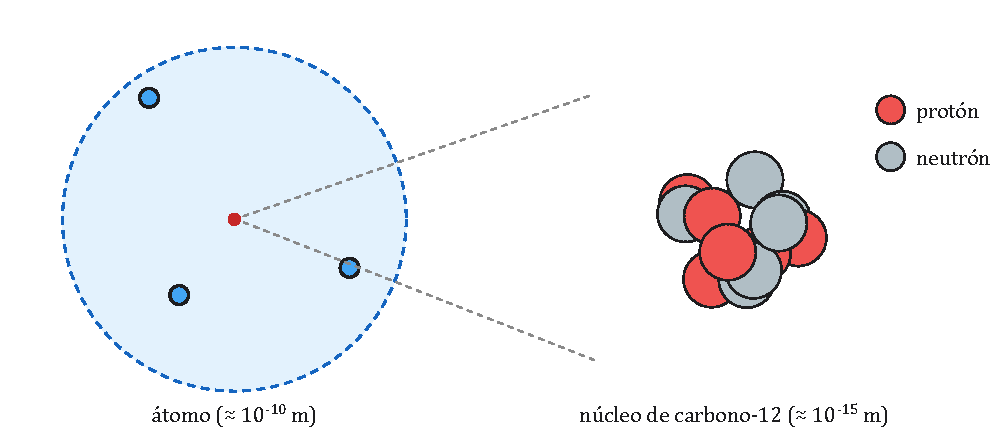
\includegraphics[width=0.75\linewidth]{images/UD8/nucleo}
    \caption{Si el átomo fuera un estadio de fútbol, el núcleo sería una canica en el centro (dibujo sin escala).}
    \label{fig:nuc-nucleo}
\end{figure}

\paragraph{Número atómico y número másico.} El \azuln{número atómico} \(Z\) es el número de protones; identifica al elemento. El
\azuln{número másico} \(A\) es el número total de nucleones, \(A = Z + N\), donde \(N\) es el número de neutrones. Un núcleo (o
\emph{nucleido}) se representa como \(\ch{^{A}_{Z}X}\): por ejemplo, \(\ch{^{235}_{92}U}\) tiene 92 protones y 143 neutrones.
\begin{itemize}
    \item \textbf{Isótopos}: mismo \(Z\) y distinto \(A\) (\ch{^{12}_{6}C} y \ch{^{14}_{6}C}). Son el mismo elemento.
    \item \textbf{Isóbaros}: mismo \(A\) y distinto \(Z\) (\ch{^{14}_{6}C} y \ch{^{14}_{7}N}).
    \item \textbf{Isótonos}: mismo número de neutrones (\ch{^{13}_{6}C} y \ch{^{14}_{7}N}).
\end{itemize}
La masa atómica de un elemento es la media ponderada de las masas de sus isótopos según su abundancia, por eso casi nunca es entera.

\paragraph{Unidad de masa atómica.} Es la doceava parte de la masa de un átomo de \ch{^{12}C}:
\(\qty{1}{u} = \dfrac{\qty{12e-3}{\kg\per\mol}}{12\cdot\qty{6.022e23}{\per\mol}} = \qty{1.66e-27}{\kg}\).

\paragraph{Tamaño del núcleo.} Los átomos miden unos \qty{e-10}{\m} y los núcleos, entre \qty{e-15}{\m} y \qty{e-14}{\m}. El radio
de un núcleo crece con la raíz cúbica de su número másico:
\begin{centeredequation}
    \boxed{R = r_0\,A^{1/3}} \qquad r_0 = \qty{1.2e-15}{\m} = \qty{1.2}{\femto\m} \label{eq:nuc-radio}
\end{centeredequation}
Como el volumen es proporcional a \(R^3\), es proporcional a \(A\): todos los núcleos tienen prácticamente la misma densidad, unos
\qty{2.3e17}{\kg\per\m\cubed}. Una cucharadita de materia nuclear pesaría más de mil millones de toneladas.

\begin{exercise}
    Calcula el radio, el volumen y la densidad de un núcleo de \ch{^{16}O}.
    \begin{solu}
        \(R = 1{,}2\cdot 10^{-15}\cdot 16^{1/3} = \textcolor{red}{\qty{3.02e-15}{\m}}\); \(V = \tfrac{4}{3}\pi R^3 = \textcolor{red}{\qty{1.16e-43}{\m\cubed}}\);
        \(\rho = \dfrac{16\cdot 1{,}66\cdot 10^{-27}}{1{,}16\cdot 10^{-43}} = \textcolor{red}{\qty{2.3e17}{\kg\per\m\cubed}}\).
    \end{solu}
\end{exercise}

\section{Las fuerzas nucleares}\label{sec:nuc-fuerzas}

Los protones del núcleo, muy próximos y con carga del mismo signo, se repelen con fuerzas eléctricas enormes. La gravedad entre
ellos es despreciable. Para que el núcleo exista tiene que haber otra interacción, atractiva y mucho más intensa: la
\rojon{interacción nuclear fuerte}. Sus características son:
\begin{itemize}
    \item Es la más intensa de las interacciones conocidas (unas 100 veces más que la eléctrica a esas distancias).
    \item Es de \textbf{muy corto alcance} (unos \qty{e-15}{\m}): cada nucleón solo atrae a sus vecinos inmediatos (\azuln{saturación}).
    \item Es \textbf{independiente de la carga}: actúa igual entre protón y protón, neutrón y neutrón, o protón y neutrón.
\end{itemize}
Los neutrones contribuyen a la atracción nuclear sin añadir repulsión eléctrica: son el «pegamento» que estabiliza los núcleos.

\section{Energía de enlace}\label{sec:nuc-enlace}

\subsection{Equivalencia entre masa y energía}\label{subsec:nuc-masa-energia}

Una de las consecuencias de la relatividad especial es que la masa es una forma de energía:
\begin{centeredequation}
    \boxed{E = m\,c^2} \label{eq:nuc-einstein}
\end{centeredequation}
En los procesos químicos los cambios de masa son imperceptibles, pero en los nucleares no: al fisionarse un gramo de uranio-235
desaparece aproximadamente un miligramo de masa, que se convierte en tanta energía como la combustión de unas tres toneladas de
carbón. Los principios de conservación de la masa y de la energía se funden en uno solo: \emph{en un sistema aislado, la suma de la
energía y del equivalente energético de la masa se conserva}.

\begin{exercise}
    Calcula, en MeV, la energía equivalente a \qty{1}{u}.
    \begin{solu}
        \(E = mc^2 = 1{,}66\cdot 10^{-27}\cdot(3\cdot 10^8)^2 = \qty{1.494e-10}{\joule} = \dfrac{1{,}494\cdot 10^{-10}}{1{,}6\cdot 10^{-13}} = \textcolor{red}{\qty{934}{\mega\electronvolt}}\).
        \textcolor{blue}{(Con valores más precisos de las constantes, \(\qty{1}{u} \equiv \qty{931.5}{\mega\electronvolt}\), que es el que usaremos.)}
    \end{solu}
\end{exercise}

\subsection{Defecto de masa y energía de enlace}\label{subsec:nuc-defecto}

Al medir con precisión la masa de un núcleo se comprueba que es \textbf{menor} que la suma de las masas de sus nucleones por
separado. La diferencia es el \rojon{defecto de masa}:
\begin{centeredequation}
    \Delta m = Z\,m_p + (A - Z)\,m_n - m_{\text{núcleo}} \label{eq:nuc-defecto}
\end{centeredequation}
Esa masa «perdida» es la energía que se libera al formarse el núcleo, la \rojon{energía de enlace}, que es también la energía mínima
necesaria para separarlo en sus nucleones:
\begin{centeredequation}
    \boxed{E_e = \Delta m\,c^2} \qquad\quad \Delta m\ (\text{en u})\ \Rightarrow\ E_e\ (\text{en MeV}) = 931{,}5\,\Delta m \label{eq:nuc-enlace}
\end{centeredequation}
Si se usa la masa del \emph{átomo} en lugar de la del núcleo, hay que tomar la del átomo de hidrógeno (\qty{1.0078}{u}) en lugar de la
del protón, para que los electrones se cancelen.

\paragraph{Energía de enlace por nucleón.} La estabilidad de un núcleo no la indica su energía de enlace total, sino la
\azuln{energía de enlace por nucleón}, \(E_e/A\): la energía media necesaria para arrancar un nucleón. Cuanto mayor es, más estable
es el núcleo (figura~\ref{fig:nuc-curva}). Crece rápidamente en los núcleos ligeros, alcanza un máximo de unos \qty{8.8}{\mega\electronvolt}
hacia el hierro-56 y desciende suavemente en los pesados.

\begin{figure}[H]
    \centering
    \begin{tikzpicture}
        \begin{axis}[fisica, width=0.8\linewidth, height=5.6cm, xmin=0, xmax=250, ymin=0, ymax=10,
            xlabel={\(A\)}, ylabel={\(E_e/A\) (\unit{\mega\electronvolt})}, xtick={50,100,150,200,250}, ytick={2,4,6,8}, samples=200]
            % fórmula semiempírica de Weizsäcker (sin término de apareamiento)
            \addplot[domain=12:240, very thick, ocre] {15.75 - 17.8/x^(1/3) - 0.711*(x/(1.98+0.015*x^(2/3)))^2/x^(4/3) - 23.7*((x-2*(x/(1.98+0.015*x^(2/3))))/x)^2};
            \addplot[only marks, mark=*, mark size=1.8pt, blue] coordinates {(2,1.11) (3,2.83) (4,7.07) (6,5.33) (7,5.61) (12,7.68) (16,7.98) (20,8.03) (56,8.79) (120,8.5) (209,7.85) (235,7.59) (238,7.57)};
            \node[font=\scriptsize, anchor=west] at (axis cs:5,7.3) {\ch{^4He}};
            \node[font=\scriptsize, anchor=south] at (axis cs:56,8.9) {\ch{^{56}Fe}};
            \node[font=\scriptsize, anchor=north] at (axis cs:235,7.4) {\ch{^{235}U}};
            \node[font=\scriptsize, anchor=west] at (axis cs:4,1.1) {\ch{^2H}};
            \draw[->, thick, red] (axis cs:20,3) -- node[below, font=\scriptsize]{fusión} (axis cs:50,3);
            \draw[->, thick, red] (axis cs:230,5) -- node[below, font=\scriptsize]{fisión} (axis cs:150,5);
        \end{axis}
    \end{tikzpicture}
    \caption{Energía de enlace por nucleón (la curva, calculada con la fórmula semiempírica; los puntos, valores medidos). Se libera
    energía al fusionar núcleos ligeros o al fisionar núcleos pesados: en los dos casos se avanza hacia el máximo.}
    \label{fig:nuc-curva}
\end{figure}

\begin{remark}
    Esta curva explica las dos fuentes de energía nuclear: al \textbf{fusionar} núcleos ligeros o al \textbf{fisionar} núcleos pesados
    se obtienen núcleos con mayor energía de enlace por nucleón, más estables, y la diferencia se libera.
\end{remark}

\begin{exercise}
    Calcula el defecto de masa, la energía de enlace y la energía de enlace por nucleón del \ch{^{23}_{11}Na}, cuya masa atómica es
    \qty{22.98977}{u} (\(m_{\text{H}} = \qty{1.0078}{u}\), \(m_n = \qty{1.0087}{u}\)).
    \begin{solu}
        \(\Delta m = 11\cdot 1{,}0078 + 12\cdot 1{,}0087 - 22{,}98977 = \textcolor{red}{\qty{0.2004}{u}}\);
        \(E_e = 0{,}2004\cdot 931{,}5 = \textcolor{red}{\qty{186.7}{\mega\electronvolt}}\);
        \(\dfrac{E_e}{A} = \textcolor{red}{\qty{8.12}{\mega\electronvolt}}\) \textcolor{blue}{por nucleón.}
    \end{solu}
\end{exercise}

\subsection{Estabilidad nuclear}\label{subsec:nuc-estabilidad}

De los más de 3000 nucleidos conocidos, solo unos 250 son estables. Si se representa el número de neutrones frente al de protones de
los núcleos estables (figura~\ref{fig:nuc-estabilidad}), se agrupan en una franja, la \azuln{banda de estabilidad}. Los núcleos ligeros
estables tienen \(N \approx Z\); los pesados necesitan cada vez más neutrones (hasta \(N/Z \approx 1{,}5\)) para compensar la repulsión
eléctrica, que crece más deprisa que la atracción nuclear. Por encima de \(Z = 83\) (bismuto) no hay núcleos estables. Los núcleos que
quedan fuera de la banda son radiactivos: se transforman hasta llegar a ella.

\begin{figure}[H]
    \centering
    \begin{tikzpicture}
        \begin{axis}[fisica, width=0.62\linewidth, height=5.6cm, xmin=0, xmax=95, ymin=0, ymax=150,
            xlabel={\(Z\)}, ylabel={\(N\)}, xtick={20,40,60,80}, ytick={40,80,120}, samples=100]
            \addplot[name path=sup, draw=none, domain=1:83] {x + 0.0075*x^2 + 2 + 0.06*x};
            \addplot[name path=inf, draw=none, domain=1:83] {x + 0.0075*x^2 - 1 + 0.01*x};
            \addplot[ocre!40] fill between[of=sup and inf];
            \addplot[domain=0:90, thick, dashed, gray] {x};
            \node[font=\scriptsize, gray, anchor=west] at (axis cs:62,58) {\(N = Z\)};
            \node[font=\scriptsize, anchor=east] at (axis cs:60,110) {banda de estabilidad};
            \node[font=\scriptsize, red, anchor=west] at (axis cs:30,85) {exceso de \(n\): \(\beta^-\)};
            \node[font=\scriptsize, blue, anchor=west] at (axis cs:55,45) {exceso de \(p\): \(\beta^+\)};
            \node[font=\scriptsize, anchor=west] at (axis cs:83,135) {\(\alpha\)};
        \end{axis}
    \end{tikzpicture}
    \caption{Banda de estabilidad. Los núcleos con demasiados neutrones emiten \(\beta^-\); los que tienen demasiados protones,
    \(\beta^+\); los muy pesados, \(\alpha\).}
    \label{fig:nuc-estabilidad}
\end{figure}

\section{La radiactividad}\label{sec:nuc-radiactividad}

La \rojon{radiactividad} es la emisión espontánea de partículas o de radiación por parte de núcleos inestables, que así se transforman
en otros más estables. No depende de la temperatura, la presión ni el estado químico: es un fenómeno puramente nuclear.

\subsection{Tipos de radiación}\label{subsec:nuc-tipos}

Si se hace pasar la radiación de una muestra radiactiva por un campo magnético, se separa en tres componentes
(figura~\ref{fig:nuc-radiaciones}):
\begin{itemize}
    \item \textbf{Radiación alfa} (\(\alpha\)): núcleos de helio, \(\ch{^4_2He}\), con carga \(+2e\). Muy ionizante y poco penetrante:
    la detiene una hoja de papel o unos centímetros de aire.
    \item \textbf{Radiación beta} (\(\beta^-\)): electrones rápidos, que \emph{no} estaban en la corteza: se crean en el núcleo al
    transformarse un neutrón en un protón. Más penetrante: la detienen unos milímetros de aluminio.
    \item \textbf{Radiación gamma} (\(\gamma\)): ondas electromagnéticas de muy alta frecuencia (fotones muy energéticos), sin carga ni
    masa. Muy penetrante: hacen falta varios centímetros de plomo o metros de hormigón para atenuarla.
\end{itemize}

\begin{figure}[H]
    \centering
    \begin{minipage}[b]{0.48\linewidth}
        \centering
        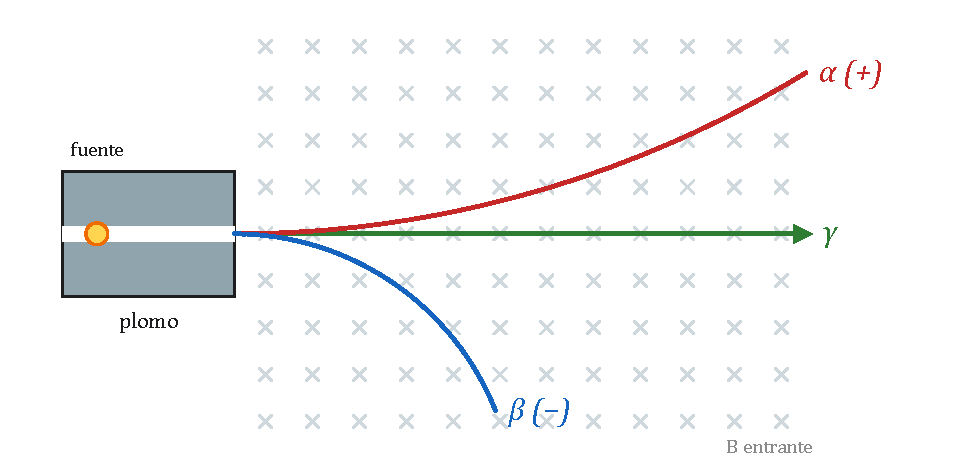
\includegraphics[width=\linewidth]{images/UD8/radiaciones}
    \end{minipage}\hfill
    \begin{minipage}[b]{0.48\linewidth}
        \centering
        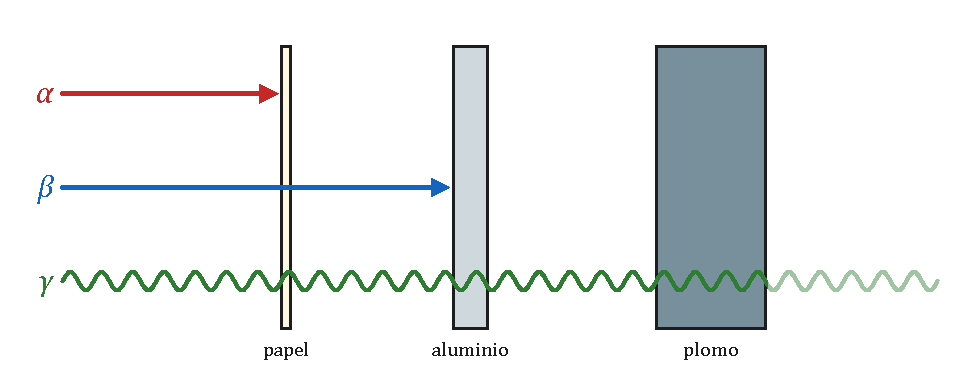
\includegraphics[width=\linewidth]{images/UD8/penetracion}
    \end{minipage}
    \caption{Izquierda: desviación de las radiaciones en un campo magnético (las \(\alpha\), mucho más pesadas, se curvan menos).
    Derecha: poder de penetración.}
    \label{fig:nuc-radiaciones}
\end{figure}

\subsection{Leyes de los desplazamientos radiactivos}\label{subsec:nuc-soddy}

En toda reacción nuclear se conservan la carga (la suma de los \(Z\)) y el número de nucleones (la suma de los \(A\)). De ahí salen las
\rojon{leyes de Soddy y Fajans}:
\begin{itemize}
    \item \textbf{Emisión \(\alpha\)}: el número atómico disminuye en 2 y el másico en 4. El elemento retrocede dos lugares en la tabla
    periódica:
    \[ \ch{^{A}_{Z}X -> ^{A-4}_{Z-2}Y + ^{4}_{2}He} \qquad\text{p. ej.}\quad \ch{^{238}_{92}U -> ^{234}_{90}Th + ^4_2He} \]
    \item \textbf{Emisión \(\beta^-\)}: un neutrón se transforma en un protón, un electrón y un antineutrino. \(Z\) aumenta en 1 y \(A\) no
    cambia; el elemento avanza un lugar:
    \[ \ch{^{A}_{Z}X -> ^{A}_{Z+1}Y + ^{0}_{-1}e} + \bar{\nu} \qquad\text{p. ej.}\quad \ch{^{14}_6C -> ^{14}_7N + ^0_{-1}e} \]
    \item \textbf{Emisión \(\beta^+\)} (radiactividad artificial): un protón se transforma en un neutrón, un positrón y un neutrino. \(Z\)
    disminuye en 1.
    \item \textbf{Emisión \(\gamma\)}: el núcleo pasa de un estado excitado a otro de menor energía; no cambian ni \(Z\) ni \(A\).
    Suele acompañar a las otras emisiones.
\end{itemize}

\begin{exercise}
    Completa las reacciones nucleares:
    \begin{enumerate}[label=\letraminuscula]
        \item \(\ch{^{14}_7N + ^4_2He -> X + ^{17}_8O}\)
        \item \(\ch{^{9}_4Be + X -> ^{12}_6C + ^1_0n}\)
        \item \(\ch{^{226}_{88}Ra -> X + ^4_2He}\)
    \end{enumerate}
    \begin{solu}
        \textcolor{blue}{Se igualan las sumas de \(A\) y de \(Z\) en los dos miembros.}
        \begin{enumerate}[label=\letraminuscula]
            \item \(A = 18 - 17 = 1\), \(Z = 9 - 8 = 1\): \(\textcolor{red}{\ch{X} = \ch{^1_1H}}\) (un protón; es la primera transmutación artificial, de Rutherford).
            \item \(A = 13 - 9 = 4\), \(Z = 6 - 4 = 2\): \(\textcolor{red}{\ch{X} = \ch{^4_2He}}\) (así descubrió Chadwick el neutrón).
            \item \(A = 222\), \(Z = 86\): \(\textcolor{red}{\ch{X} = \ch{^{222}_{86}Rn}}\).
        \end{enumerate}
    \end{solu}
\end{exercise}

\subsection{Ley de la desintegración radiactiva}\label{subsec:nuc-ley}

La desintegración es un proceso \textbf{aleatorio}: no se puede saber cuándo se desintegrará un núcleo concreto, solo la probabilidad de
que lo haga. En una muestra con \(N\) núcleos, el número que se desintegra en un tiempo \(dt\) es proporcional a \(N\) y a \(dt\):
\begin{equation*}
    dN = -\lambda\,N\,dt \qquad\Rightarrow\qquad \int_{N_0}^{N}\dfrac{dN}{N} = -\lambda\int_0^t dt \qquad\Rightarrow\qquad \ln\dfrac{N}{N_0} = -\lambda t
\end{equation*}
\begin{centeredequation}
    \boxed{N = N_0\,e^{-\lambda t}} \label{eq:nuc-ley}
\end{centeredequation}
\(\lambda\) es la \azuln{constante de desintegración} (\unit{\per\second}), característica de cada nucleido: es la probabilidad de que un
núcleo se desintegre por unidad de tiempo. La misma ley vale para la masa de la muestra, \(m = m_0 e^{-\lambda t}\).

\paragraph{Actividad.} La \rojon{actividad} es el número de desintegraciones por unidad de tiempo:
\begin{centeredequation}
    \boxed{A = \left|\dfrac{dN}{dt}\right| = \lambda\,N} \qquad\Rightarrow\qquad A = A_0\,e^{-\lambda t} \label{eq:nuc-actividad}
\end{centeredequation}
Su unidad en el SI es el \azuln{becquerel} (\(\qty{1}{\becquerel}\) = una desintegración por segundo). También se usa el
\emph{curio}: \(\qty{1}{Ci} = \qty{3.7e10}{\becquerel}\) (la actividad de un gramo de radio).

\paragraph{Período de semidesintegración y vida media.} El \rojon{período de semidesintegración} \(T_{1/2}\) es el tiempo que tarda en
desintegrarse la mitad de los núcleos. Haciendo \(N = N_0/2\):
\begin{centeredequation}
    \dfrac{1}{2} = e^{-\lambda T_{1/2}} \qquad\Rightarrow\qquad \boxed{T_{1/2} = \dfrac{\ln 2}{\lambda}} \label{eq:nuc-semi}
\end{centeredequation}
Al cabo de \(n\) períodos quedan \(N_0/2^n\) núcleos (figura~\ref{fig:nuc-ley}). La \rojon{vida media} \(\tau\) es el tiempo medio que
vive un núcleo antes de desintegrarse: \(\boxed{\tau = 1/\lambda}\), y por tanto \(T_{1/2} = \tau\ln 2 = 0{,}693\,\tau\). Los períodos
van desde fracciones de microsegundo hasta miles de millones de años (\ch{^{238}U}: \num{4.5e9} años).

\begin{figure}[H]
    \centering
    \begin{tikzpicture}
        \begin{axis}[fisica, width=0.62\linewidth, height=5cm, xmin=0, xmax=4.6, ymin=0, ymax=1.15,
            xlabel={\(t\)}, ylabel={\(N\)}, xtick={1,2,3,4}, xticklabels={\(T_{1/2}\),\(2T_{1/2}\),\(3T_{1/2}\),\(4T_{1/2}\)},
            ytick={0.125,0.25,0.5,1}, yticklabels={\(\frac{N_0}{8}\),\(\frac{N_0}{4}\),\(\frac{N_0}{2}\),\(N_0\)}, samples=120]
            \addplot[domain=0:4.4, very thick, ocre] {2^(-x)};
            \draw[dashed, gray] (axis cs:0,0.5) -- (axis cs:1,0.5) -- (axis cs:1,0);
            \draw[dashed, gray] (axis cs:0,0.25) -- (axis cs:2,0.25) -- (axis cs:2,0);
            \draw[dashed, gray] (axis cs:0,0.125) -- (axis cs:3,0.125) -- (axis cs:3,0);
        \end{axis}
    \end{tikzpicture}
    \caption{Ley de la desintegración radiactiva: en cada período de semidesintegración queda la mitad de los núcleos.}
    \label{fig:nuc-ley}
\end{figure}

\begin{exercise}
    El período de semidesintegración del \ch{^{32}_{15}P} es de \qty{14.3}{días}. ¿Cuánto tiempo tiene que pasar para que se desintegre el
    \qty{90}{\percent} de una muestra? ¿Cuál es su vida media?
    \begin{solu}
        \textcolor{blue}{\(\lambda = \ln 2/14{,}3 = \qty{0.0485}{\per\day}\). Si se desintegra el \qty{90}{\percent}, queda \(N = 0{,}1N_0\):}
        \(t = \dfrac{\ln 10}{\lambda} = \textcolor{red}{\qty{47.5}{días}}\); \(\tau = \dfrac{1}{\lambda} = \textcolor{red}{\qty{20.6}{días}}\).
    \end{solu}
\end{exercise}

\begin{exercise}
    Un isótopo tiene un período de semidesintegración de \qty{50}{\second}. Una muestra que contenía al principio \(10^{10}\) núcleos tiene
    ahora \(10^8\). Calcula la antigüedad de la muestra, su vida media y su actividad dentro de \qty{500}{\second}.
    \begin{solu}
        \textcolor{blue}{\(\lambda = \ln 2/50 = \qty{0.01386}{\per\second}\).}
        \(t = \dfrac{\ln(N_0/N)}{\lambda} = \dfrac{\ln 100}{0{,}01386} = \textcolor{red}{\qty{332}{\second}}\); \(\tau = \textcolor{red}{\qty{72.1}{\second}}\).

        \(A = \lambda N_0' e^{-\lambda t} = 0{,}01386\cdot 10^8\cdot e^{-6{,}93} = \textcolor{red}{\qty{1.35e3}{\becquerel}}\).
    \end{solu}
\end{exercise}

\begin{exercise}
    El \ch{^{226}_{88}Ra} tiene un período de semidesintegración de 1600 años. Calcula la actividad de \qty{1}{\mg} de este isótopo.
    \begin{solu}
        \(\lambda = \dfrac{\ln 2}{1600\cdot 3{,}156\cdot 10^7} = \qty{1.37e-11}{\per\second}\);
        \(N = \dfrac{10^{-3}}{226}\cdot 6{,}022\cdot 10^{23} = \num{2.66e18}\).
        \(A = \lambda N = \textcolor{red}{\qty{3.66e7}{\becquerel}}\) \textcolor{blue}{(prácticamente un milicurio).}
    \end{solu}
\end{exercise}

\paragraph{Datación con carbono-14.} En la atmósfera se forma continuamente \ch{^{14}C}, radiactivo (\(T_{1/2} = 5730\) años). Mientras
un ser vivo vive, intercambia carbono con el medio y la proporción de \ch{^{14}C} se mantiene constante; al morir, deja de incorporarlo y
el \ch{^{14}C} empieza a desintegrarse. Midiendo la actividad de una muestra y comparándola con la de una muestra viva se obtiene su
antigüedad, hasta unos 50\,000 años.

\section{Reacciones nucleares. Fisión y fusión}\label{sec:nuc-reacciones}

En una reacción nuclear la energía liberada (\(Q\)) se obtiene de la diferencia de masas entre reactivos y productos:
\begin{centeredequation}
    Q = \left(\sum m_{\text{reactivos}} - \sum m_{\text{productos}}\right)c^2 \label{eq:nuc-Q}
\end{centeredequation}

\subsection{Fisión nuclear}\label{subsec:nuc-fision}

La \rojon{fisión} es la ruptura de un núcleo pesado en dos núcleos de masa intermedia, al absorber un neutrón. Con el uranio-235, por
ejemplo (figura~\ref{fig:nuc-fision}):
\[ \ch{^{235}_{92}U + ^1_0n -> ^{144}_{56}Ba + ^{89}_{36}Kr + 3 ^1_0n} \]
Se pueden formar muchos pares de productos distintos (todos radiactivos), se liberan entre 2 y 3 neutrones y unos \qty{200}{\mega\electronvolt}
por fisión, que se convierten en calor.

\begin{figure}[H]
    \centering
    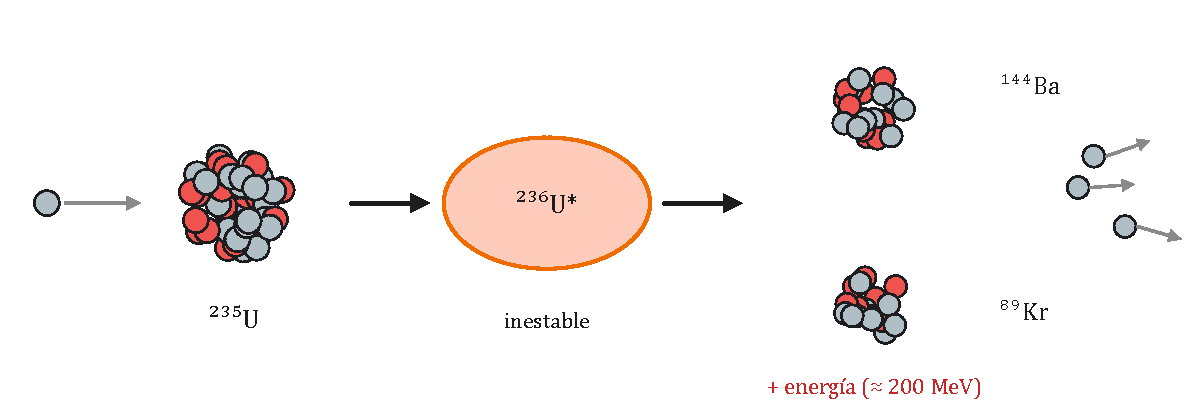
\includegraphics[width=0.85\linewidth]{images/UD8/fision}
    \caption{Fisión del uranio-235 inducida por un neutrón lento.}
    \label{fig:nuc-fision}
\end{figure}

\paragraph{Reacción en cadena y masa crítica.} Los neutrones liberados pueden provocar nuevas fisiones, que liberan más neutrones, y así
sucesivamente: es una \azuln{reacción en cadena} (figura~\ref{fig:nuc-cadena}). Para que se mantenga, la muestra tiene que superar una
\azuln{masa crítica}; si es más pequeña, demasiados neutrones escapan por la superficie.

\begin{figure}[H]
    \centering
    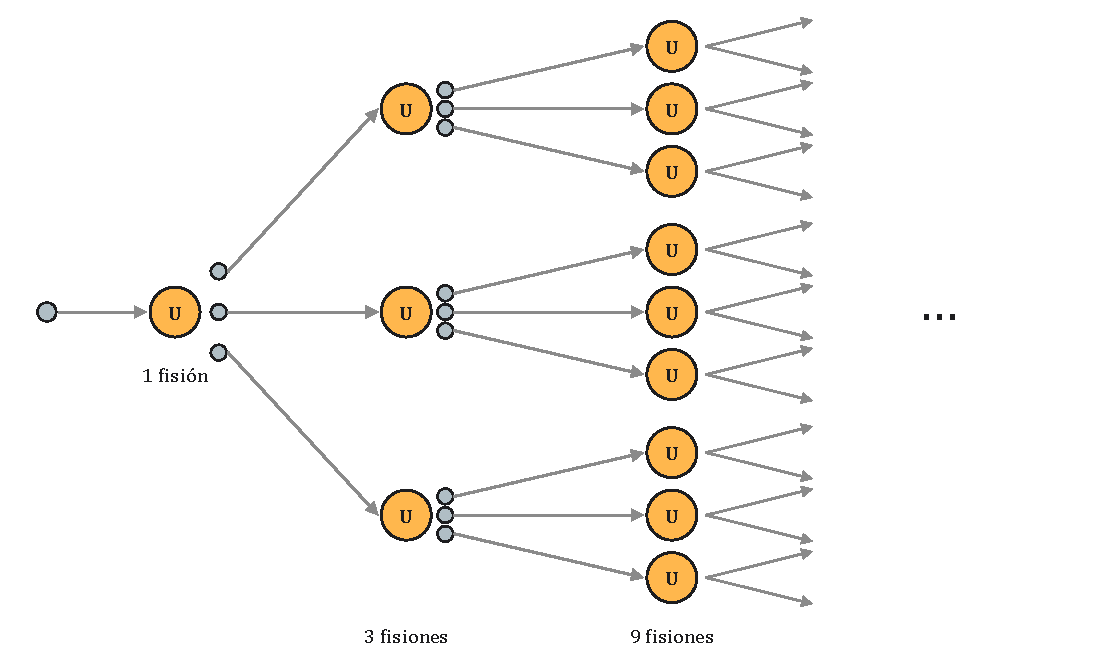
\includegraphics[width=0.66\linewidth]{images/UD8/cadena}
    \caption{Reacción en cadena: si cada fisión provoca, de media, más de una fisión nueva, el número de fisiones crece exponencialmente.}
    \label{fig:nuc-cadena}
\end{figure}

\paragraph{Reactores nucleares.} En un reactor la reacción en cadena se mantiene controlada, de modo que cada fisión provoca exactamente
otra (figura~\ref{fig:nuc-reactor}). Sus partes principales son:
\begin{itemize}
    \item el \textbf{combustible} (uranio enriquecido en \ch{^{235}U}), en barras;
    \item el \textbf{moderador} (agua, agua pesada o grafito), que frena los neutrones para que provoquen fisiones con más facilidad;
    \item las \textbf{barras de control} (cadmio o boro), que absorben neutrones y regulan la reacción;
    \item el \textbf{refrigerante}, que extrae el calor y lo lleva al generador de vapor; el vapor mueve una turbina unida a un alternador;
    \item el \textbf{reflector} y el \textbf{blindaje}, que devuelven los neutrones al núcleo y protegen de la radiación.
\end{itemize}
Si la reacción no se controla y se libera toda la energía en un instante, se tiene una bomba atómica.

\begin{figure}[H]
    \centering
    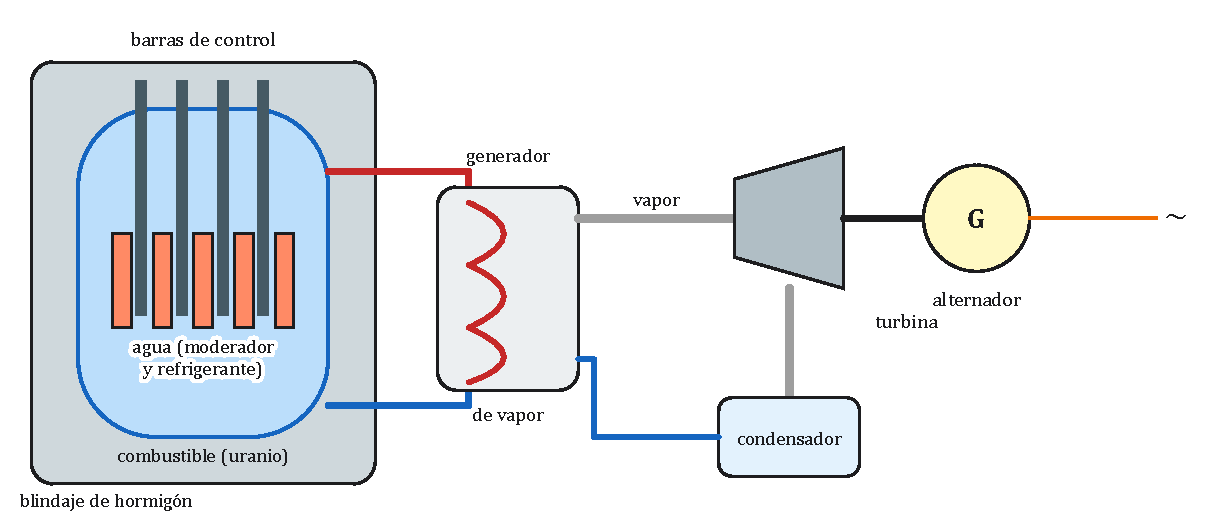
\includegraphics[width=0.85\linewidth]{images/UD8/reactor}
    \caption{Esquema simplificado de una central nuclear de agua a presión.}
    \label{fig:nuc-reactor}
\end{figure}

\begin{exercise}
    En la fisión \(\ch{^{235}_{92}U + ^1_0n -> ^{94}_{38}Sr + ^{140}_{54}Xe + 2 ^1_0n}\), calcula la energía liberada por cada núcleo
    fisionado y la masa de uranio-235 que consume en una hora una central de \qty{3000}{\mega\watt} térmicos. Masas: U-235,
    \qty{235.0439}{u}; Sr-94, \qty{93.9154}{u}; Xe-140, \qty{139.9216}{u}; neutrón, \qty{1.0087}{u}.
    \begin{solu}
        \(\Delta m = 235{,}0439 + 1{,}0087 - 93{,}9154 - 139{,}9216 - 2\cdot 1{,}0087 = \qty{0.1982}{u}\);
        \(Q = 0{,}1982\cdot 931{,}5 = \textcolor{red}{\qty{184.6}{\mega\electronvolt}}\).

        \textcolor{blue}{Energía en una hora: \(3\cdot 10^9\cdot 3600 = \qty{1.08e13}{\joule}\); núcleos: \(\dfrac{1{,}08\cdot 10^{13}}{184{,}6\cdot 1{,}6\cdot 10^{-13}} = \num{3.66e23}\).}
        \(m = \dfrac{3{,}66\cdot 10^{23}}{6{,}022\cdot 10^{23}}\cdot 235 = \textcolor{red}{\qty{143}{\g}}\) \textcolor{blue}{(una central de carbón quemaría más de 1000 toneladas).}
    \end{solu}
\end{exercise}

\subsection{Fusión nuclear}\label{subsec:nuc-fusion}

La \rojon{fusión} es la unión de dos núcleos ligeros para formar uno más pesado. Por ejemplo, la de deuterio y tritio
(figura~\ref{fig:nuc-fusion}):
\[ \ch{^2_1H + ^3_1H -> ^4_2He + ^1_0n} \qquad Q = \qty{17.6}{\mega\electronvolt} \]
Por gramo de combustible libera unas cuatro veces más energía que la fisión. Es la fuente de energía de las estrellas: el Sol fusiona
cada segundo unos 600 millones de toneladas de hidrógeno en helio.

\begin{figure}[H]
    \centering
    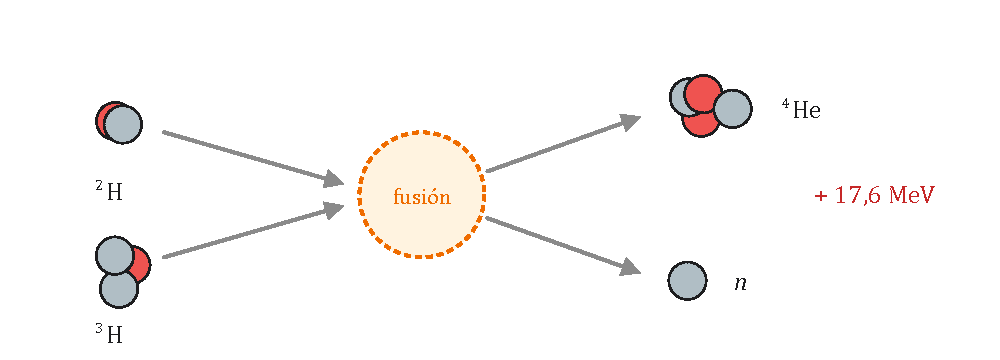
\includegraphics[width=0.66\linewidth]{images/UD8/fusion}
    \caption{Fusión de deuterio y tritio.}
    \label{fig:nuc-fusion}
\end{figure}

Para que dos núcleos se fusionen tienen que vencer su repulsión eléctrica, lo que exige temperaturas de unos cien millones de grados. A
esas temperaturas la materia es un \azuln{plasma} (núcleos y electrones separados) que ningún recipiente puede contener. Se investigan dos
formas de confinarlo: el \emph{confinamiento magnético}, con campos magnéticos intensos en reactores de tipo tokamak (como el proyecto
internacional ITER), y el \emph{confinamiento inercial}, comprimiendo pequeñas cápsulas de combustible con láseres muy potentes.

\begin{remark}
    \textbf{Ventajas de la fusión}: combustible casi inagotable (el deuterio se extrae del agua del mar y el tritio se obtiene del litio),
    no produce residuos radiactivos de larga duración y no hay riesgo de reacción descontrolada. \textbf{Inconvenientes}: todavía no se ha
    conseguido producir más energía de la que se consume de forma sostenida; los neutrones vuelven radiactivos los materiales del reactor,
    y las instalaciones son enormemente caras y complejas.
\end{remark}

\section{Radiactividad artificial y aplicaciones}\label{sec:nuc-aplicaciones}

En 1934, Irène Curie y Frédéric Joliot bombardearon aluminio con partículas alfa y obtuvieron un isótopo radiactivo del fósforo que no
existe en la naturaleza:
\[ \ch{^{27}_{13}Al + ^4_2He -> ^{30}_{15}P + ^1_0n} \qquad\qquad \ch{^{30}_{15}P -> ^{30}_{14}Si + ^0_{1}e} \]
Era la primera \textbf{radiactividad artificial}, y en ella aparece la emisión de positrones (\(\beta^+\)). Hoy los
\azuln{radioisótopos} se fabrican sobre todo en reactores, bombardeando núcleos estables con neutrones, y tienen muchas aplicaciones:

\begin{table}[H]
    \centering
    \caption{Aplicaciones de algunos radioisótopos}
    \vspace{-5pt}
    \begin{tabular}{@{}lL{10.4cm}@{}}
        \toprule
        \textbf{Isótopo} & \textbf{Aplicación} \\
        \midrule
        Yodo-131 & Diagnóstico y tratamiento de enfermedades del tiroides \\[3pt]
        Cobalto-60 & Radioterapia contra el cáncer; esterilización de material quirúrgico y de alimentos \\[3pt]
        Tecnecio-99m & Gammagrafías (el isótopo más usado en medicina nuclear) \\[3pt]
        Flúor-18 & Tomografía por emisión de positrones (PET) \\[3pt]
        Carbono-14 & Datación de restos orgánicos \\[3pt]
        Hidrógeno-3 (tritio) & Trazador en estudios del agua; señales luminosas \\[3pt]
        Fósforo-32 & Trazador en biología y agricultura (absorción de fertilizantes) \\[3pt]
        Americio-241 & Detectores de humo \\
        \bottomrule
    \end{tabular}
    \label{tab:nuc-aplicaciones}
\end{table}

\paragraph{Efectos biológicos y dosis.} Las radiaciones ionizantes pueden dañar las células y el ADN. Para medir sus efectos se usan:
\begin{itemize}
    \item la \azuln{dosis absorbida}, energía absorbida por kilogramo de tejido, medida en \emph{grays} (\(\qty{1}{Gy} = \qty{1}{\joule\per\kg}\));
    \item la \azuln{dosis equivalente}, que multiplica la anterior por un factor que tiene en cuenta el tipo de radiación (1 para \(\beta\)
    y \(\gamma\), 20 para \(\alpha\)), medida en \emph{sieverts} (\unit{Sv}).
\end{itemize}
Recibimos de forma natural (rayos cósmicos, radón del suelo, alimentos) unos \qty{2.4}{mSv} al año; una radiografía de tórax supone unos
\qty{0.1}{mSv}. El límite recomendado para la población, además de la radiación natural, es de \qty{1}{mSv} al año. Para protegerse de una
fuente radiactiva hay tres reglas: \textbf{distancia}, \textbf{tiempo} de exposición corto y \textbf{blindaje}.

\section{Resumen de fórmulas}\label{sec:nuc-resumen}

\begin{table}[H]
    \centering
    \caption{Fórmulas principales de la física nuclear}
    \vspace{-5pt}
    \begin{tabular}{@{}lL{10cm}@{}}
        \toprule
        \textbf{Magnitud} & \textbf{Expresión} \\
        \midrule
        Núcleo & \(A = Z + N\), \quad \(R = r_0 A^{1/3}\), \quad \(r_0 = \qty{1.2e-15}{\m}\) \\[3pt]
        Masa y energía & \(E = mc^2\), \quad \(\qty{1}{u} = \qty{1.66e-27}{\kg} \equiv \qty{931.5}{\mega\electronvolt}\) \\[3pt]
        Energía de enlace & \(\Delta m = Z m_p + N m_n - m_{\text{núcleo}}\), \quad \(E_e = \Delta m\,c^2\), \quad \(E_e/A\) \\[3pt]
        Desplazamientos & \(\alpha\): \(Z - 2\), \(A - 4\); \quad \(\beta^-\): \(Z + 1\); \quad \(\beta^+\): \(Z - 1\); \quad \(\gamma\): sin cambio \\[3pt]
        Desintegración & \(N = N_0 e^{-\lambda t}\), \quad \(A = \lambda N = A_0 e^{-\lambda t}\) \\[3pt]
        Período y vida media & \(T_{1/2} = \ln 2/\lambda\), \quad \(\tau = 1/\lambda\) \\[3pt]
        Energía de una reacción & \(Q = (\sum m_{\text{reactivos}} - \sum m_{\text{productos}})\,c^2\) \\
        \bottomrule
    \end{tabular}
    \label{tab:nuc-resumen}
\end{table}

\section{Prácticas}\label{sec:nuc-practicas}

\subsection{Práctica 1: simulación de la desintegración con dados}\label{subsec:nuc-practica-dados}

\textbf{Objetivo.} Comprobar el carácter aleatorio de la desintegración y obtener la ley exponencial y el período de semidesintegración.

\textbf{Material.} Unos 100 dados (o monedas, o caramelos con una cara marcada) y una caja.

\textbf{Procedimiento.}
\begin{enumerate}[label=\numberballmDarkTeal]
    \item Cada dado es un «núcleo». Lánzalos todos: los que saquen un 6 se han «desintegrado» y se retiran. Anota cuántos quedan.
    \item Repite con los que quedan hasta que queden muy pocos. Cada lanzamiento es una unidad de tiempo.
    \item Junta los datos de toda la clase para tener más núcleos.
\end{enumerate}

\textbf{Cálculos y cuestiones.}
\begin{enumerate}[label=\letraminuscula]
    \item Representa \(N\) frente al número de lanzamientos y \(\ln N\) frente al número de lanzamientos. ¿Qué forma tienen las gráficas?
    \item La pendiente de la segunda es \(-\lambda\). Compárala con la probabilidad de sacar un 6 (\(1/6\)) y calcula \(T_{1/2}\).
    \item ¿Puedes predecir qué dado concreto se «desintegrará» en el siguiente lanzamiento? ¿Y cuántos lo harán, aproximadamente?
\end{enumerate}

\subsection{Práctica 2: radiactividad ambiental}\label{subsec:nuc-practica-contador}

\textbf{Objetivo.} Medir la radiación de fondo y comprobar cómo varía con la distancia y con el blindaje.

\textbf{Material.} Contador Geiger (o la aplicación de un móvil con un detector adaptado), fuentes de muy baja actividad de uso escolar o
materiales naturalmente radiactivos (fertilizante de potasio, sal sin sodio, granito), láminas de papel, aluminio y plomo.

\textbf{Procedimiento.}
\begin{enumerate}[label=\numberballmDarkTeal]
    \item Mide el número de cuentas por minuto sin ninguna fuente, varias veces: es la radiación de fondo.
    \item Coloca la muestra a distintas distancias del detector y mide las cuentas (restando el fondo).
    \item Interpón papel, aluminio y plomo entre la muestra y el detector y anota cómo cambian las cuentas.
\end{enumerate}

\textbf{Cuestiones.}
\begin{enumerate}[label=\letraminuscula]
    \item ¿Por qué el número de cuentas no es exactamente igual en medidas repetidas?
    \item ¿Cómo varían las cuentas con la distancia? ¿Se parece a \(1/r^2\)?
    \item A partir de los blindajes, ¿qué tipo de radiación emite la muestra? Relaciónalo con las tres reglas de protección.
\end{enumerate}


    \newpage

    %! Unidad 8 — Física nuclear: ejercicios finales (adaptados de la fuente, con datos cambiados y resueltos)

\section{Ejercicios}\label{sec:nuc-ejercicios}

Salvo que se indique otra cosa, usa \(c = \qty{3e8}{\m\per\second}\), \(\qty{1}{u} = \qty{1.66e-27}{\kg} \equiv \qty{931.5}{\mega\electronvolt}\),
\(m_{\text{H}} = \qty{1.0078}{u}\), \(m_n = \qty{1.0087}{u}\), \(N_A = \qty{6.022e23}{\per\mol}\), \(\qty{1}{\mega\electronvolt} = \qty{1.6e-13}{\joule}\)
y \(r_0 = \qty{1.2e-15}{\m}\).

\subsection{El núcleo y la energía de enlace}

\begin{exercise}
    Calcula el radio y el volumen de un núcleo de \ch{^7Li}.
    \begin{solu}
        \(R = r_0 A^{1/3} = 1{,}2\cdot 10^{-15}\cdot 7^{1/3} = \textcolor{red}{\qty{2.30e-15}{\m}}\); \(V = \tfrac{4}{3}\pi R^3 = \textcolor{red}{\qty{5.07e-44}{\m\cubed}}\).
    \end{solu}
\end{exercise}

\begin{exercise}
    Un núcleo tiene tantos protones como neutrones y su radio es la mitad del radio del \ch{^{64}Cu}. ¿De qué núcleo se trata?
    \begin{solu}
        \textcolor{blue}{\(R \propto A^{1/3}\): si el radio es la mitad, \(A = 64/2^3 = 8\), con \(Z = N = 4\).} \textcolor{red}{Es el \ch{^8_4Be}}
        \textcolor{blue}{(muy inestable: se rompe en dos partículas alfa).}
    \end{solu}
\end{exercise}

\begin{exercise}
    Calcula el radio del \ch{^{30}P} y del \ch{^{235}U} y estima la densidad de la materia nuclear.
    \begin{solu}
        \(R_P = 1{,}2\cdot 10^{-15}\cdot 30^{1/3} = \textcolor{red}{\qty{3.73e-15}{\m}}\); \(R_U = \textcolor{red}{\qty{7.41e-15}{\m}}\).

        \(\rho = \dfrac{A\,u}{\tfrac{4}{3}\pi r_0^3 A} = \dfrac{1{,}66\cdot 10^{-27}}{\tfrac{4}{3}\pi(1{,}2\cdot 10^{-15})^3} = \textcolor{red}{\qty{2.3e17}{\kg\per\m\cubed}}\) \textcolor{blue}{(la misma para todos).}
    \end{solu}
\end{exercise}

\begin{exercise}
    Calcula la energía de enlace y la energía de enlace por nucleón del \ch{^4_2He} y del \ch{^{16}_8O}, cuyas masas atómicas son
    \qty{4.0026}{u} y \qty{15.9949}{u}. ¿Cuál es más estable?
    \begin{solu}
        \ch{^4He}: \(\Delta m = 2\cdot 1{,}0078 + 2\cdot 1{,}0087 - 4{,}0026 = \qty{0.0304}{u}\); \(E_e = \textcolor{red}{\qty{28.3}{\mega\electronvolt}}\), \(E_e/A = \textcolor{red}{\qty{7.08}{\mega\electronvolt}}\).

        \ch{^{16}O}: \(\Delta m = 8\cdot 1{,}0078 + 8\cdot 1{,}0087 - 15{,}9949 = \qty{0.1371}{u}\); \(E_e = \textcolor{red}{\qty{127.7}{\mega\electronvolt}}\), \(E_e/A = \textcolor{red}{\qty{7.98}{\mega\electronvolt}}\).

        \textcolor{red}{El oxígeno-16 es más estable} \textcolor{blue}{(mayor energía de enlace por nucleón).}
    \end{solu}
\end{exercise}

\begin{exercise}
    ¿Qué energía se libera, por núcleo, en una reacción nuclear con un defecto de masa de \qty{0.2}{u}?
    \begin{solu}
        \(E = \Delta m\,c^2 = 0{,}2\cdot 1{,}66\cdot 10^{-27}\cdot 9\cdot 10^{16} = \textcolor{red}{\qty{2.99e-11}{\joule}} \approx \textcolor{red}{\qty{186}{\mega\electronvolt}}\).
    \end{solu}
\end{exercise}

\subsection{Radiactividad y reacciones nucleares}

\begin{exercise}
    ¿Cuántas partículas \(\alpha\) y \(\beta^-\) emite un núcleo de \ch{^{238}_{92}U} hasta convertirse en \ch{^{206}_{82}Pb}?
    \begin{solu}
        \textcolor{blue}{Solo las \(\alpha\) cambian \(A\): \((238 - 206)/4 = 8\) partículas \(\alpha\), que reducen \(Z\) en 16. Como \(Z\) solo baja de 92 a 82 (10
        unidades), las \(\beta^-\) lo aumentan en \(16 - 10 = 6\).} \textcolor{red}{8 partículas \(\alpha\) y 6 partículas \(\beta^-\).}
    \end{solu}
\end{exercise}

\begin{exercise}
    Un núcleo de \ch{^{181}_{73}Ta} se bombardea con un protón y emite 4 neutrones. ¿Qué número atómico y másico tiene el núcleo resultante?
    \begin{solu}
        \textcolor{blue}{\(A = 181 + 1 - 4 = 178\); \(Z = 73 + 1 = 74\).} \textcolor{red}{Es el \ch{^{178}_{74}W}} \textcolor{blue}{(wolframio).}
    \end{solu}
\end{exercise}

\begin{exercise}
    Un núcleo \ch{X} con \(Z = 90\) y \(A = 232\) emite una partícula \(\alpha\) y se transforma en \ch{Y}, que a su vez emite una partícula
    \(\beta^-\) y se transforma en \ch{Z}. ¿Qué números atómico y másico tiene \ch{Z}?
    \begin{solu}
        \textcolor{blue}{Tras la \(\alpha\): \(Z = 88\), \(A = 228\). Tras la \(\beta^-\): \(Z = 89\), \(A = 228\).} \textcolor{red}{\(Z = 89\), \(A = 228\)} \textcolor{blue}{(actinio).}
    \end{solu}
\end{exercise}

\begin{exercise}
    Completa las reacciones nucleares:
    \begin{enumerate}[label=\letraminuscula]
        \item \(\ch{^1_0n + ^{59}_{27}Co -> ^{60}_{27}Co} + \mathrm{X}\)
        \item \(\ch{^{234}_{90}Th -> ^{234}_{91}Pa} + \mathrm{X}\)
        \item \(\ch{^1_0n + ^{115}_{49}In} \rightarrow \mathrm{X} + \gamma\)
        \item \(\ch{^{12}_6C} + \mathrm{X} \rightarrow \ch{^9_4Be + ^4_2He}\)
    \end{enumerate}
    \begin{solu}
        \begin{enumerate}[label=\letraminuscula]
            \item \textcolor{red}{\(\gamma\)} \textcolor{blue}{(no cambian ni \(A\) ni \(Z\))}.
            \item \textcolor{red}{\(\ch{^0_{-1}e}\)} \textcolor{blue}{(emisión \(\beta^-\))}.
            \item \textcolor{red}{\(\ch{^{116}_{49}In}\)}.
            \item \textcolor{red}{\(\ch{^1_0n}\)} \textcolor{blue}{(\(A\): \(13 - 12 = 1\); \(Z\): \(6 - 6 = 0\))}.
        \end{enumerate}
    \end{solu}
\end{exercise}

\begin{exercise}
    Calcula la energía liberada en la desintegración \(\ch{^{226}Ra -> ^{222}Rn + ^4He}\). Masas: \qty{225.9771}{u}, \qty{221.9703}{u} y \qty{4.0026}{u}.
    \begin{solu}
        \(\Delta m = 225{,}9771 - 221{,}9703 - 4{,}0026 = \qty{0.0042}{u}\); \(Q = 0{,}0042\cdot 931{,}5 = \textcolor{red}{\qty{3.9}{\mega\electronvolt}}\).
    \end{solu}
\end{exercise}

\begin{exercise}
    En la reacción \(\ch{^{A}_{Z}Li + ^1_1H -> 2 ^4_2He}\) se liberan \qty{17.35}{\mega\electronvolt}. Calcula \(Z\) y \(A\) del litio y su masa atómica.
    \begin{solu}
        \textcolor{blue}{\(A + 1 = 8\), \(Z + 1 = 4\):} \(\textcolor{red}{\ch{^7_3Li}}\).
        \(m_{\text{Li}} = 2\cdot 4{,}0026 + \dfrac{17{,}35}{931{,}5} - 1{,}0078 = \textcolor{red}{\qty{7.016}{u}}\).
    \end{solu}
\end{exercise}

\subsection{Ley de la desintegración}

\begin{exercise}
    El \ch{^{210}_{84}Po} tiene un período de semidesintegración de 138 días. ¿Qué masa de este isótopo tiene una actividad de \qty{2e7}{\becquerel}?
    \begin{solu}
        \(\lambda = \dfrac{\ln 2}{138\cdot 86400} = \qty{5.81e-8}{\per\second}\); \(N = \dfrac{A}{\lambda} = \num{3.44e14}\);
        \(m = \dfrac{N}{N_A}\cdot 210 = \textcolor{red}{\qty{1.2e-7}{\g}}\) \textcolor{blue}{(0,12 microgramos).}
    \end{solu}
\end{exercise}

\begin{exercise}
    La actividad de una muestra pasa de \qty{1500}{\becquerel} a \qty{1470}{\becquerel} en un día. Calcula el período de semidesintegración
    y el número de núcleos en cada momento.
    \begin{solu}
        \(\lambda = \dfrac{\ln(1500/1470)}{86400} = \qty{2.34e-7}{\per\second}\); \(T_{1/2} = \dfrac{\ln 2}{\lambda} = \textcolor{red}{\qty{34.3}{días}}\).
        \(N_0 = \dfrac{A_0}{\lambda} = \textcolor{red}{\num{6.42e9}}\); \(N = \textcolor{red}{\num{6.29e9}}\).
    \end{solu}
\end{exercise}

\begin{exercise}
    En 4 meses se ha desintegrado el \qty{5}{\percent} de una muestra radiactiva. Calcula su período de semidesintegración y su vida media.
    \begin{solu}
        \(\lambda = \dfrac{-\ln 0{,}95}{4} = 0{,}01282\ \text{mes}^{-1}\); \(T_{1/2} = \dfrac{\ln 2}{\lambda} = \textcolor{red}{\num{54.1}\ \text{meses}}\);
        \(\tau = \dfrac{1}{\lambda} = \textcolor{red}{\num{78.0}\ \text{meses}}\).
    \end{solu}
\end{exercise}

\begin{exercise}
    El yodo-131 tiene un período de semidesintegración de 8 días. Hoy tenemos \qty{40}{\mg}. ¿Qué cantidad había hace 24 días? ¿Cuánto quedará
    dentro de 24 días?
    \begin{solu}
        \textcolor{blue}{24 días son 3 períodos.} Hace 24 días: \(40\cdot 2^3 = \textcolor{red}{\qty{320}{\mg}}\); dentro de 24 días: \(40/2^3 = \textcolor{red}{\qty{5}{\mg}}\).
    \end{solu}
\end{exercise}

\begin{exercise}
    Un isótopo tiene un período de semidesintegración de \qty{15}{\hour}. ¿Cuánto tarda en desintegrarse el \qty{93.75}{\percent} de una muestra?
    ¿Cuál es su vida media?
    \begin{solu}
        \textcolor{blue}{Queda \(0{,}0625 = 1/16 = 1/2^4\): han pasado 4 períodos.} \(t = \textcolor{red}{\qty{60}{\hour}}\); \(\tau = \dfrac{T_{1/2}}{\ln 2} = \textcolor{red}{\qty{21.6}{\hour}}\).
    \end{solu}
\end{exercise}

\begin{exercise}
    La actividad del \ch{^{14}C} de un trozo de madera antigua es la octava parte de la de una muestra de madera actual de la misma masa. ¿Qué
    antigüedad tiene? (\(T_{1/2} = 5730\) años).
    \begin{solu}
        \textcolor{blue}{\(1/8 = 1/2^3\): han pasado 3 períodos.} \(t = 3\cdot 5730 = \textcolor{red}{17\,190\ \text{años}}\).
    \end{solu}
\end{exercise}

\begin{exercise}
    El \ch{^{212}_{83}Bi} tiene un período de semidesintegración de \qty{60.5}{\minute}. ¿Cuántos átomos se desintegran por segundo en \qty{40}{\g} de este isótopo?
    \begin{solu}
        \(\lambda = \dfrac{\ln 2}{60{,}5\cdot 60} = \qty{1.91e-4}{\per\second}\); \(N = \dfrac{40}{212}\cdot 6{,}022\cdot 10^{23} = \num{1.14e23}\);
        \(A = \lambda N = \textcolor{red}{\qty{2.17e19}{\becquerel}}\).
    \end{solu}
\end{exercise}

\begin{exercise}
    El período de semidesintegración del polonio-210 es de 138 días. Si tenemos \qty{1}{\mg}, ¿al cabo de cuánto tiempo quedarán \qty{0.25}{\mg}?
    \begin{solu}
        \textcolor{blue}{Queda la cuarta parte: 2 períodos.} \(t = \textcolor{red}{276\ \text{días}}\).
    \end{solu}
\end{exercise}

\subsection{Fisión y fusión}

\begin{exercise}
    La fisión de un núcleo de uranio-235 libera unos \qty{200}{\mega\electronvolt}. ¿Cuánto tiempo tarda en consumir \qty{20}{\kg} de uranio-235 un
    reactor de \qty{1000}{\mega\watt}?
    \begin{solu}
        \(N = \dfrac{20\,000}{235}\cdot 6{,}022\cdot 10^{23} = \num{5.13e25}\) núcleos; \(E = N\cdot 200\cdot 1{,}6\cdot 10^{-13} = \qty{1.64e15}{\joule}\).
        \(t = \dfrac{E}{P} = \qty{1.64e6}{\second} = \textcolor{red}{\num{19.0}\ \text{días}}\).
    \end{solu}
\end{exercise}

\begin{exercise}
    La combustión de \qty{1}{\kg} de carbón proporciona \qty{3.3e7}{\joule}. ¿Qué masa de carbón da la misma energía que la fisión de
    \qty{235}{\g} de uranio-235 (\qty{200}{\mega\electronvolt} por núcleo)?
    \begin{solu}
        \textcolor{blue}{235 g son un mol: \(E = 6{,}022\cdot 10^{23}\cdot 200\cdot 1{,}6\cdot 10^{-13} = \qty{1.93e13}{\joule}\).}
        \(m = \dfrac{1{,}93\cdot 10^{13}}{3{,}3\cdot 10^7} = \textcolor{red}{\qty{5.8e5}{\kg}}\) \textcolor{blue}{(casi 600 toneladas).}
    \end{solu}
\end{exercise}

\begin{exercise}
    Una central de fusión funcionaría con la reacción \(\ch{^2H + ^2H -> ^4He}\), con un rendimiento del \qty{35}{\percent}. ¿Qué masa de deuterio
    necesitaría para producir \qty{2e6}{\kilo\watt\hour} de energía eléctrica? Masas: \ch{^2H}, \qty{2.0141}{u}; \ch{^4He}, \qty{4.0026}{u}.
    \begin{solu}
        \(\Delta m = 2\cdot 2{,}0141 - 4{,}0026 = \qty{0.0256}{u}\); \(Q = \qty{23.8}{\mega\electronvolt} = \qty{3.82e-12}{\joule}\) por reacción.

        \textcolor{blue}{Energía térmica necesaria: \(\dfrac{2\cdot 10^6\cdot 3{,}6\cdot 10^6}{0{,}35} = \qty{2.06e13}{\joule}\); reacciones: \num{5.39e24}, cada una con dos deuterones.}
        \(m = 2\cdot 5{,}39\cdot 10^{24}\cdot 2{,}0141\cdot 1{,}66\cdot 10^{-27} = \textcolor{red}{\qty{36}{\g}}\).
    \end{solu}
\end{exercise}


%----------------------------------------------------------------------------------------
%	SOLUCIONES
%----------------------------------------------------------------------------------------

    \part{Soluciones a los ejercicios}

    \chapterimage{images/portada_cabeceras/cabecera_general}
    \chapter{Soluciones}

    \pagestyle{fancy}

    \Closesolutionfile{ans}

    \IfFileExists{soluciones2BachFis.tex}{\input{soluciones2BachFis}}{}

\end{document}
